%------------------------------- CHAPTER NAME --------------------------------
\chapter{Take-off and Landing performance}
\label{chap:TakeOff}

\begin{flushright}
	{\smaller
		\textit{When everything seems to be going against you, \\ remember that the airplane takes off against the wind, not with it.}\\
		-- Henry Ford}
\end{flushright}

\noindent
Although the take-off field length may seem like a performance characteristic of secondary importance, it is very often one of the critical design constraints. If the required runway length is too long, the aircraft cannot take-off with full fuel or full payload and its economics are compromised.
%
So take-off performance play a significant role in both the conceptual and the preliminary design phases of an aircraft because it is both design requirement, specified by the \gls{FAR} and by the customer, to be fulfilled, both a driving parameter in the definition of the design point. If the take-off performance is important, as it provides a limitation both in the wing loading $\frac{W}{S}$, both in the $\frac{T}{W}$ (or the $\frac{W}{P}$) ratio, also the landing performance is crucial as it imposes another limitation on the wing loading inside the design point definition.
%
%-------------------------- THEORETICAL BACKGROUND ---------------------------
\section{Theoretical background}
%
\begin{figure}[!t]
\centering
\includegraphics[keepaspectratio, width=0.97\textwidth]{TakeOffRun}
\caption{Scheme of an aircraft take-off run}
\label{fig:TOrun}
\end{figure}
%
The take-off may be considered as made up of two parts: a ground run and an air run, as shown schematically in figure~\ref{fig:TOrun}. The simplest description of the take-off process is that the engine thrust is increased to the take-off level at x = 0 and the brakes are released to begin acceleration down the runway. At some point, the pilot commands rotation of the aircraft which lifts the nose wheel from the ground and allows to achieve the take-off angle of attack; in this way the aircraft lift can grows faster and, when it is equal to the aircraft maximum take-off weight, the aircraft can lifts completely from the ground and begins climbing. The point at which it reaches an altitude of 35 \si{ft} (10.7 \si{\meter}), is considered, for an aircraft which refers to the \gls{FAR}-25, the end of the take-off run. 
%
This is the usual situation for take-off; subsequently, the modifications to safely deal with a take-off emergency, such as an engine failure, will be discussed.
%
%-----------------------------AOE Take-Off subsection-----------------------------
\subsection{\gls{acr:AOE} take-off run}
In order to deal with the calculation of the take-off run distance, a smart strategy is to find out all the fundamentals variables, which describes completely the aircraft state in this phase, and so, to study the dynamic system in exam in a state-space representation.
%
\noindent
To find out these state variables it is necessary to analyze aircraft equations of motion during take-off phases, these latter described as follows.
\begin{itemize}
\item \textbf{Ground roll phase}: starting from standstill with brakes released and at maximum power output, the aircraft accelerates on the runway, with constant angle of attack, until it reaches a speed equals to the rotation speed V\textsubscript{Rot}; after that the following sub-phase begin.
%
\begin{itemize}
\item \textbf{Rotation phase}: a short phase in which the pilot gives an assigned pitching law to lift the aircraft nose and, as a result, increasing the angle of attack. This phase ends when the load factor is equal to 1, meaning that the lift has reached the value of the maximum take-off weight, and the relative lift-off speed is indicated with V\textsubscript{LO}. 
%
\end{itemize}
%
\item \textbf{Airborne phase}: is the phases in which the aircraft, once it has lifted from the ground, gains altitude until it reaches the obstacle height of 35 \si{ft} (10.7 \si{\meter}) imposed by the \gls{FAR}-25. This phase begin at V\textsubscript{LO} and ends at the speed related to the obstacle overcoming, indicated with V\textsubscript{2}; furthermore it can be divided into the followings two sub-phases:
%
\begin{itemize}
\item \textbf{Transition phase}: in which the aircraft rotates in order to increase the climb angle ($\gamma$) with the result of increasing the angle of attack and the relative lift coefficient, which should not surpass a safety value of the 90\% of the maximum lift coefficient in take-off configuration. This sub-phase ends when the desired climb speed is reached.
%
\item \textbf{Climb-out to the obstacle phase}: in which the aircraft climbs at constant climb angle until the obstacle is surpassed.
\end{itemize}
\end{itemize}
%
\noindent
For more information regarding take-off equations of motion during each of the previously described phases, the reader can refer to~\cite{McCormick}.

\bigskip
\noindent
The set of \gls{acr:ODE} that models the take-off run is written in the following form:
%
\begin{equation}\label{eq:Take:Off:System:Dynamics:A}
    \LEFTRIGHT\lcbrace\rcbrace{\begin{array}{c}\dot{s}\\[2pt] \dot{V} \\[2pt] \dot{\gamma} \\[2pt] \dot{h} \end{array}}
= 
    \LEFTRIGHT\lcbrace\rcbrace{\begin{array}{l}
       f_1 \big(\, s,\, V,\, \gamma,\, h \,; \, \alpha \big) \\[4pt]
       f_2 \big(\, s,\, V,\, \gamma,\, h \,; \, \alpha \big) \\[4pt]
       f_3 \big(\, s,\, V,\, \gamma,\, h \,; \, \alpha \big) \\[4pt]
       f_4 \big(\, s,\, V,\, \gamma,\, h \,; \, \alpha \big)
    \end{array}}
\qquad
    \text{with}\quad
    \LEFTRIGHT\lcbrace.{\begin{array}{l} x_1 = s\\[2pt] x_2 = V \\[2pt] x_3 = \gamma \\[2pt] x_4 = h \end{array}}
\qquad
    \text{and}\quad
    u = \alpha
\end{equation}
%
\noindent
These equations can be also written in a more concise way as shown below.
%
\begin{equation}
\label{eq:Take:Off:System:Dynamics:B}
\dot{\vec{x}} = \vec{f}\big(\, \vec{x}\,;\,u \,\big)
\end{equation}
%
\noindent
The unknown $\vec{x} = [\mspace{2mu} x_1,\, x_2,\, x_3,\, x_4 \mspace{2mu}]^{\text{T}}$ is the vector of state variables. The input $u(t)$ is a given function of time, for $0 \leq t \leq t_{\text{final}}$, that corresponds to an assumed time history of the angle of attack during take-off.
%
The right-hand sides of system (\ref{eq:Take:Off:System:Dynamics:A}) are defined by the following functions:
%
\begin{subequations}\label{eq:Take:Off:System:Dynamics:RHS:functions}
\begin{equation}\label{eq:Take:Off:System:Dynamics:RHS:functions:A}
f_1 \big(\, \vec{x}\,,\,u \,\big) =  x_2
\end{equation}
%
\begin{equation}\label{eq:Take:Off:System:Dynamics:RHS:functions:B}
f_2 \big(\, \vec{x}\,,\,u \,\big) =
  \frac{g}{W}
    \LEFTRIGHT\lcbrace.{
      \begin{array}{l@{\rule{2em}{0pt}}l} 
        T(x_2) - D(x_2,u) - \mu \big[ W - L(x_2,u) \big]
          & \text{if} \;\, \mathcal{S}(x_2 , u) < 1
        \\[1em]
        T(x_2) \cos u - D(x_2,u) - W \sin x_3
          & \text{if} \;\, \mathcal{S}(x_2 , u) \geq 1
      \end{array}
    }  
\end{equation}
%
\begin{equation}\label{eq:Take:Off:System:Dynamics:RHS:functions:C}
f_3 \big(\, \vec{x}\,,\,u \,\big) =
  \frac{g}{W\,x_2}
    \LEFTRIGHT\lcbrace.{
      \begin{array}{l@{\rule{2em}{0pt}}l} 
        0
          & \text{if} \;\, \mathcal{S}(x_2 , u) < 1
        \\[1em]
        L(x_2,u) + T(x_2)\sin u - W \cos x_3
          & \text{if} \;\, \mathcal{S}(x_2 , u) \geq 1
      \end{array}
    }  
\end{equation}
%
\begin{equation}\label{eq:Take:Off:System:Dynamics:RHS:functions:D}
f_4 \big(\, \vec{x}\,,\,u \,\big) =  x_2 \, \sin x_3
\end{equation}
%
\noindent
The thrust $T(x_2)$ is calculated by means of the interpolating function $T_{\text{tab}}\big(V_{\text{a}}\big)$ based on a table lookup algorithm, where $V_{\text{a}} = V + V_{\text{w}}$ is the airspeed and $V_{\text{w}}$ is the wind speed (horizontal component, positive if opposite to the aircraft motion).
%
The drag $D$ and lift $L$, as functions of airspeed $V_{\text{a}}$ and angle of attack, are given by the following conventional formulas.
%
\begin{equation}\label{eq:Take:Off:System:Dynamics:RHS:functions:E}
D(x_2,u) = \frac{1}{2} \, \rho \, \big( x_2 + V_{\text{w}}\cos x_3 \big)^2 \,S \, C_D\big( u \big)
\end{equation}
%
\begin{equation}\label{eq:Take:Off:System:Dynamics:RHS:functions:E}
L(x_2,u) = \frac{1}{2} \, \rho \, \big( x_2 + V_{\text{w}}\cos x_3 \big)^2 \,S \, C_L\big( u \big)
\end{equation}
%
\noindent
The switching function $\mathcal{S}$ of aircraft velocity and angle of attack is defined as follows:
%
\begin{equation}\label{eq:Take:Off:System:Dynamics:RHS:functions:D}
\mathcal{S}(x_2 , u) = \frac{L(x_2,u)}{W \cos x_3}
\end{equation}
\end{subequations}
%
\noindent
The formulas (\ref{eq:Take:Off:System:Dynamics:RHS:functions}) make the system (\ref{eq:Take:Off:System:Dynamics:B})  a closed set of \gls{acr:ODE}.
%
\noindent
When the function $u(t)$ is assigned and the system is associated to a set of initial conditions, in this particular case equal to $\vec{x}_0 = [\mspace{2mu} 0,\, 0,\, 0,\, 0 \mspace{2mu}]^{\text{T}}$, a well-posed \gls{acr:IVP} is formed, which can be solved numerically.
%
In table~\ref{tab:Take:Off:Speeds:FAR25} are reported the take-off characteristic speeds and their corresponding requirements as defined by \gls{FAR}-25.
%
\begingroup
\begin{longtable}[H]{lll}
\label{tab:Take:Off:Speeds:FAR25}\\
\toprule
Speed & Description & Requirement
\\ \midrule
\endfirsthead
%
\multicolumn{3}{l}%
  {\relsize{-1}({\itshape continued from previous page})}\\
\toprule
Speed & Description & Requirement
\\ \midrule
\endhead
%
\midrule \multicolumn{3}{r}{{\relsize{-1}\itshape continued on next page}}
\endfoot
%
\bottomrule
\caption[Take-off speeds and FAR~25 requirements]{Take-off speeds and FAR~25 requirements}
\endlastfoot
%
$V_\mathrm{S}$ & aircraft stalling speed in take-off configuration & ---
\\
$V_\mathrm{MC}$ & minimum control speed with one engine inoperative (OEI) & ---
\\
$V_1$ & OEI decision speed & $\geq V_\mathrm{mc}$
\\
$V_\mathrm{Rot}$ & rotation speed & $>1.05\, V_\mathrm{MC}$
\\
$V_\mathrm{MU}$ & minimum unstick speed for safe flight & $\geq V_\mathrm{S}$
\\
$V_\mathrm{LO}$ & lift-off speed & $> 1.10 \, V_\mathrm{MU}$
\\
                &                & $> 1.05 \, V_\mathrm{MU}$ (OEI)
\\
$V_2$ & take-off climb speed at \SI[round-precision=0]{35}{ft} & $> 1.20 \, V_\mathrm{S}$
\\
                &                & $> 1.10 \, V_\mathrm{MC}$
\end{longtable}
\endgroup
%
\noindent
It has to be highlighted that the drag coefficient $C_D$ that appears in (\ref{eq:Take:Off:System:Dynamics:RHS:functions:E}) can be modeled as:
%
\begin{equation}\label{eq:CD:A}
C_D = C_{D0} + \left(\upDelta C_{D0}\right)_{\text{flap}+\text{lg}} +  K_g\ \frac{C_L^2}{\pi \AR e}
\end{equation}
%
with $\left(\upDelta C_{D0}\right)_{\text{flap}+\text{lg}}$ due to flap, as shown in subparagraph~\ref{subpar:DCD0}, and landing gears, which contribution is usually about $0.010 \div 0.015$; moreover $C_L$ is the one from the lift curve with flaps, and eventually slats, deflected. The term $K_g$ in (\ref{eq:CD:A}) incorporates the ground effect and it is calculated from~\cite{McCormick} using the (\ref{eqn:FifthOrderPoly}) which is a fifth order interpolating function of the  graph in figure~\ref{fig:McCormickGroundEffect}, where the ratio $h_{\text{W}}/b$ is obtained dividing the height of wing above the ground by the wing span, usually between 0.1 and 0.2 when the aircraft is on the ground and assumed as $h_{\text{W}} \approx h$ during the airborne.
%
\begin{figure}[H]
\centering
\includegraphics[keepaspectratio, width=0.57\textwidth]{McCormickGroundEffect}
\caption{Ground effect parameter $K_g$ as function of the $h_{\text{W}}/b$ ratio}
\label{fig:McCormickGroundEffect}
\end{figure}
%
\begin{equation}
K_g=-622.44x^5+624.46x^4-255.24x^3+47.105x^2-0.6378x+0.0055
\label{eqn:FifthOrderPoly}
\end{equation}
%
This polynomial equation has a coefficient of determination $R^2$ of 0.9999 which justifies the approximation.
%
\begin{figure}[!t]
\centering
\includegraphics[keepaspectratio, width=\textwidth]{GroundEffect}
\caption{Comparison between flight with and without ground effect}
\label{fig:GroundEffect}
\end{figure}

\bigskip
\noindent
In order to better understand the nature of the ground effect it is convenient to refer to~\cite{nicolai2010fundamentals}, where the ground effect is explained as follows.
%
As the aircraft flies close to the ground, the ground interferes with the horseshoe vortex system trailing behind the wing. Ground effect is often analyzed by putting an image horseshoe vortex system of equal but opposite strength at the same distance $h_{\text{W}}$ below the ground.
%
This image vortex system induces velocities at the wing aerodynamic center, which decreases the strength of the downwash at that point, thereby decreasing the induced angle of attack, $\alpha_i$. Thus, the wing $C_L$ is increased (or more correctly, the lift curve slope increases, giving an increase in $C_L$ for the same geometric angle of attack, $\alpha$) and the induced drag is decreased.
%
This influence of the ground effect is a function of how close the aircraft is to the ground and of the size of the wing.

\bigskip
\noindent
Speaking of the $C_D$, it has also to be noted that, at high $C_L$, the parabolic drag polar it's no longer accurate in describing the drag characteristics of the aircraft so that two correction factors have to be added to the (\ref{eq:CD:A}). These latter triggers only when the $C_L$ is higher than 1.2, as can be seen from the following equation, in which $K_1$ and $K_2$ values depend on the aircraft in exam.
%
\begin{equation}
C_D = C_{D0} + \left(\upDelta C_{D0}\right)_{\text{flap}+\text{lg}} +  K_g\ \frac{C_L^2}{\pi \AR e} + K_1\ \left(C_L-1.2\right) + K_2\ \left(C_L-1.2\right)^2
\end{equation}

\bigskip
\noindent
Focusing, now, on the input law of the angle of attack, the function $u$ can be constructed by picking the time $t_{\text{Rot}}$ when the rotation speed $V_{\text{Rot}}$ is reached along the ground roll; thus the $u (t)$ function can be defined as follows.

\bigskip
\begin{equation}\label{eq:Take:Off:System:Dynamics:Alpha:Law}
u (t) =
    \LEFTRIGHT\lcbrace.{
      \begin{array}{l@{\rule{2em}{0pt}}l} 
        \alpha_{\text{g}}
          & \text{if} \;\, t < t_{\text{Rot}}
        \\[1em]
        \alpha_1(t)
          & \text{if} \;\, t \geq t_{\text{Rot}}
      \end{array}
    }
\end{equation}
%
with a constant $\alpha_{\text{g}}$ during the ground run up to the rotation speed, and a given non-zero law $\alpha_1(t)$ for the post-rotation angle of attack time history. 
%
\begin{figure}[!t]
\centering
\includegraphics[keepaspectratio, width=0.45\textwidth]{AlphaInputTakeOff}
\caption{Qualitative representation of the angle of attack input law}
\label{fig:AlphaInput}
\end{figure}
%
Figure~\ref{fig:AlphaInput} shows a qualitative representation of the $\alpha_1(t)$ law. As can be seen, after $t_{\text{Rot}}$ the pilot applies an initial angular velocity $\dot\alpha_{0}$, which decreases with time, according to the law written in (\ref{eqn:AlphaDot}) as function of $\alpha$, until the time $t_{\text{Hold}}$ has been reached; this particular instant is related to the achievement of the maximum admitted lift coefficient in take-off, which is set at 90\% of the $C_{L\text{max,TO}}$.
%
\begin{equation}
\dot\alpha=\dot\alpha_0\ \left(1-k_\alpha\ \alpha\right)
\label{eqn:AlphaDot}
\end{equation}
%
\noindent
In equation (\ref{eqn:AlphaDot}), the $k_\alpha$ slope is assigned (expressed in $\si{1/\degree}$ and dependent on the aircraft in exam), while the initial angular velocity $\dot\alpha_0$ is calculated as follows.
%
\begin{equation}
\dot\alpha_0=\dfrac{\upDelta\alpha}{\upDelta t_{\text{Rot}}}=\dfrac{\alpha_{\text{LO}}-\alpha_g}{\upDelta t_{\text{Rot}}}
\label{eqn:AlphaDotInitial}
\end{equation}
%
where $\alpha_{\text{LO}}$ can be obtained from the lift curve of the wing, with flaps deflected in take-off configuration, by assigning the $C_{\text{L}_{\text{LO}}}$; this can be derived from the $C_{L\text{max,TO}}$ dividing it by the parameter $K^2_{\text{LO}}$, which represents the quantity that has to be multiplied by $V_{\text{S}}$ in order to obtain $V_{\text{LO}}$ (for example 1.1 with reference to table~\ref{tab:Take:Off:Speeds:FAR25}).

\bigskip
\noindent
From this point on the pilot stops the pitching maneuver and keeps the angle of attack constant for an assigned $\upDelta t_{\text{Hold}}$. During this time interval, the lift coefficient is high and, as a result, also the induced drag is high so that aircraft acceleration will reduce. 
%
After this short time interval the pilot has to reduce the angle of attack in order to avoid the acceleration to decrease too much and so an assigned negative angular velocity $\dot\alpha_{\text{red}}$ is applied; the latter assumed to be constant for simplicity. 
%
Finally, since the decrease of $\alpha$ determines also a reduction in $C_L$, the time $t_{\text{climb}}$ will be reached when the load factor is reduced to 1; this means that a balance of the forces, perpendicular to the flight path, has been achieved and so the climb phase, at constant $\gamma$, can begin, leaving $\alpha$ constant and equal to last value reached. Moreover, from this time on, the lift value is constant and equal to $W\cdot\cos\gamma$, in order to maintain the load factor equal to 1; while the $C_L$ is derived from the lift value using the (\ref{eqn:Lift.Equation}).
%
%-----------------------------OEI Take-Off subsection-----------------------------
\subsection{\gls{acr:OEI} take-off run and balanced field length}
\label{subpar:OEI}
A good description of the take-off with one engine failure is proposed in \cite{sforza2014commercial}. Here it is explained that in the event of an engine failure during the take-off roll the pilot must decide whether to continue the take-off or, instead, abort the take-off and decelerate to a stop on the runway. Obviously, if the engine failure occurs when the aircraft is traveling very slowly, the aircraft should be kept on the ground and brought to a stop at some safe location off the runway. Conversely, if the engine failure occurs when the aircraft is close to the take-off speed the take-off should be continued. The designer must provide a means for deciding whether it is safer to abort the take-off or continue it.
%
The critical velocity, denoted as $V_{\text{act}}$, is the velocity at which action is taken, not that at which the decision to act is taken. The time between the recognition of an engine failure, which occurs at $V_{\text{ef}}$, and the critical velocity $V_{\text{act}}$, when action is taken is required to be more than one second. Generally this time period, which is set by the reaction time of the pilot, is taken to be about \SI{3}{\second}. If the pilot decision is to continue the take-off with one engine inoperative, the distance to the lift-off speed $V_{\text{LO}}$ and to the subsequent climb-out to 35 $\si{ft}$ height above the runway, will obviously be longer than with all engines operating.

\bigskip
\noindent
The calculation of the take-off distance in this situation is quite the same as the one explained previously, with the difference that now there is a discontinuity in thrust due to the broken engine. In particular, the thrust, $T(x_2)$, will still be read from the database but considering a number of engines reduced by one from the time $t_{\text{ef}}$ at which the engine failure occurs.

\bigskip
\noindent
On the other hand, in the case of the aborted take-off the pilot will apply the necessary braking procedures in order to get the maximum permissible deceleration while maintaining adequate control of the airplane motion. The portion of the aborted take-off run up to the engine failure velocity $V_{\text{ef}}$ is calculated in the same way as that for the continued take-off, so that the distance is the same in both cases. 
%
From this point on, until the pilot reacts by activating brakes, there is only a discontinuity in thrust due to the failed engine; while, after the time interval in which the pilot decides to abort the take-off, the thrust is set to minimum (ideally zero) and the brakes action provides an higher friction coefficient. During this last phase, the equation (\ref{eq:Take:Off:System:Dynamics:RHS:functions:B}) changes in the following.
%
\begin{equation}\label{eq:Take:Off:System:Dynamics:RHS:functions:Aborted}
f_2 \big(\, \vec{x}\,,\,u \,\big) =\frac{g}{W}\ \big\{ - D(x_2,u) - \mu_{\text{brakes}} \big[ W - L(x_2,u) \big]\big\} 
\end{equation}
%
where $\mu_{\text{brakes}}$ is bigger than $\mu$ and it is usually about 0.3.
%
Furthermore, it has to be noted that, even if the aircraft in exam is supplied with a reverse thrust device, this effect has not to be taken into account for a more conservative result. 

\bigskip
\noindent
Instead of considering the limiting cases of aborting take-off at low $V_{\text{act}}$ and continued take-off at high $V_{\text{act}}$, it is useful determine the critical velocity for which the distance required to continue the take-off is equal to the distance required to safely abort it. This velocity is the one from table \ref{tab:Take:Off:Speeds:FAR25} and it's called \emph{decision speed} $V_1$, while the related distance is called the \emph{balanced field length}. The latter, in particular, plays an important role in the sizing of the runway since is the maximal distance the aircraft can cover both in continued take-off, both in 
aborted take-off. 
%
In order to calculate this distance, and the related velocity, it's possible to evaluate, at different $V_{\text{act}}$,  both the continued take-off distance with one inoperative engine, both the aborted take-off distance. Each couple of speed and distance can then be plotted with the result of building the curves of figure~\ref{fig:BalancedFieldLength}. The intersection of these latter, at which the two distances are the same, defines the \emph{balanced field length} and the $V_1$.
%
\begin{figure}[H]
\centering
\includegraphics[keepaspectratio, width=0.6\textwidth]{BalancedFieldLength}
\caption{Qualitative representation of the field distances required to continue a takeoff or to abort it when one
engine fails as a function of critical velocity}
\label{fig:BalancedFieldLength}
\end{figure}
%
\noindent
As expected, the take-off distance on the curve related to the continued take-off with one inoperative engine decreases with the failure speed, tending to the \gls{acr:AOE} condition; while the take-off distance on the other curve grows with the failure speed because the deceleration to stop the aircraft begins from an higher speed, requiring more distance to be dissipated.
%
%----------------------------------- Landing subsection---------------------------------------
\subsection{Landing distance calculation}
Similar to the take-off, the landing phase can be considered as made up of two main components: an air run and a ground run as shown in figure \ref{fig:LANDrun}. A comprehensive description of these two phases is provided by \cite{sforza2014commercial} and it is reported below.
%
\begin{figure}[!t]
\centering
\includegraphics[keepaspectratio, width=0.97\textwidth]{LandingRun}
\caption{Scheme of an aircraft landing run}
\label{fig:LANDrun}
\end{figure}

\bigskip
\noindent
The air run may be considered to start at the an obstacle height of $\SI{50}{\foot}$, so that in an x-y coordinate system with x = 0 at y = $\SI{50}{\foot}$, the approach speed equals $V_A$, which, according to \gls{FAR}, must be at least 1.3 $V_s$ in landing configuration. The aircraft executes a gradual flare of large radius $R$, turning the pitch angle from $\theta$ around $\SI{2}{\degree}$ or $\SI{3}{\degree}$ down to zero at which time the aircraft has slowed to $V_{\text{Flare}}$, that is, to a value around $1.2\div1.25 V_s$ (in landing configuration) and settled onto the runway, ending the air run at x = $S_A+S_{\text{Flare}}$ as shown in figure \ref{fig:LANDairborne}. To calculate this distance the simplest way is to assume that the flare rotation describes a circular trajectory and that $\theta_a$, during approach is small and almost equal to $\theta_f$. By using these hypotheses the two distances $S_A$ and $S_{\text{Flare}}$ can be calculated through a geometrical approach which follows the steps below. 
%
\begin{figure}[!b]
\centering
\includegraphics[keepaspectratio, width=0.7\textwidth]{LandingAirborne}
\caption{Scheme of the air run of the landing phase}
\label{fig:LANDairborne}
\end{figure}
%
\begin{itemize}
%
\item Assuming a load factor $n=1.2$ and a $V_{\text{Flare}}$ equal to the mean value between $V_A=1.3\ V_s$ and $V_{\text{TD}}=1.15\ V_s$ ($V_{\text{Flare}}=1.23\ V_s$, the radius $R$ can be calculated as 
\begin{equation}
R=\dfrac{V^2}{g\left(n-1\right)}=\dfrac{V_{\text{Flare}}^2}{0.2\ g}
\label{eqn:Landing:Airborne:A}
\end{equation}
\noindent
where $g$ is the gravitational constant. 
%
\item With a $\theta_a$ around  $\SI{2}{\degree}$ or $\SI{3}{\degree}$, it's possible to calculate the flare height from ground as follows.
\begin{equation}
h_{\text{Flare}}=R\left(1-\cos\theta_a\right)
\label{eqn:Landing:Airborne:B}
\end{equation}
%
\item At this point, known $\theta_a$, $R$ and $h_{\text{Flare}}$, the two distances can be calculated as follows.
\begin{equation}
S_A=\dfrac{50-h_{\text{Flare}}}{\tan\theta_a}; \quad\quad S_{\text{Flare}}=R\sin\theta_a
\label{eqn:Landing:Airborne:C}
\end{equation}
%
\end{itemize}
%

\bigskip
\noindent
The ground run begins when the aircraft touches the ground and ends when the speed is equal to zero; the first part of the ground run is named \emph{free-roll distance}, which lasts around $\SI{3}{\second}$, and represents the distance covered while the pilot reduces the power to idle, retracts the flaps, deploys the spoilers, and applies the brakes. The second part of the ground run is almost the same described during the aborted take-off with the difference that now there is no engine failure and the focus is on the decelerated trait.

\bigskip
\noindent
Also in this case the description of the aircraft motion can be easily carried out integrating an appropriate set of \gls{acr:ODE}, which are describe below.
%
\begin{equation}\label{eq:Landing:System:Dynamics:A}
    \LEFTRIGHT\lcbrace\rcbrace{\begin{array}{c}\dot{s}\\[2pt] \dot{V} \end{array}}
= 
    \LEFTRIGHT\lcbrace\rcbrace{\begin{array}{l}
       f_1 \big(\, s,\, V \big) \\[4pt]
       f_2 \big(\, s,\, V \big) \\[4pt]
    \end{array}}
\qquad
    \text{with}\quad \vec{x} = 
    \LEFTRIGHT\lcbrace.{\begin{array}{l} x_1 = s\\[2pt] x_2 = V \end{array}}
\end{equation}
%
\noindent
where the right-hand sides of system (\ref{eq:Landing:System:Dynamics:A}) are defined by the following functions:
%
\begin{subequations}\label{eq:Landing:System:Dynamics:RHS:functions}
\begin{equation}\label{eq:Landing:System:Dynamics:RHS:functions:A}
f_1 \big(\, \vec{x}\,\big) =  x_2
\end{equation}
%
\begin{equation}\label{eq:Take:Off:System:Dynamics:RHS:functions:B}
f_2 \big(\, \vec{x}\,\big) =
  \frac{g}{W}
    \LEFTRIGHT\lcbrace.{
      \begin{array}{l@{\rule{2em}{0pt}}l} 
        -T_{\text{Rev}}(x_2) - D(x_2) - \mu \big[ W - L(x_2) \big]
          & \text{if} \;\, t \leqslant t_{\text{fr}}
        \\[1em]
	-T_{\text{Rev}}(x_2) - D(x_2) - \mu_{\text{brakes}} \big[ W - L(x_2) \big]
          & \text{if} \;\, t > t_{\text{fr}}
      \end{array}
    }  
\end{equation}
\end{subequations}
%
The drag and lift values are calculated in the same way of the take-off ground roll, while $T_{\text{Rev}}$ is a reverse thrust produced by thrust reversers, for jet engine, or by a particular regulation of the blade pass, for a propeller engine. The latter is usually neglected for the ground distance calculation because it helps the deceleration of the aircraft, but for more clarity, it has been considered in the equation. Furthermore the instant $t_{\text{fr}}$ is related to the end of the \emph{free-roll distance} and it's set at \SI{3}{\second} as explained before.

\bigskip
\noindent
When both the ground distance, both the airborne phase distance are calculated, it's finally possible to determine the total landing distance by summing these latter.
%------------------------- JAVA CLASS ARCHITECTURE ---------------------------
\section{Java class architecture}
%
Now that the theoretical background is fully described, it's time to analyze the structure of the Java classes implemented inside \gls{JPAD} dedicated to the calculation of the take-off and landing distances.
%
%----------------------------------------- Take-Off ------------------------------------
\subsection{Take-Off}
As in previous chapters, a dedicated Java class, named~\lstinline[language=Java]!CalcTakeOff!, has been created to manage all required methods. The first component to be described is the class constructor; the latter, in addition to linking all the input parameter to the related class fields, provides a series of preliminary calculations which defines other required input data, not given from the user, such as the maximum lift coefficient in take-off configuration, or the stalling speed in take-off, and some of the characteristic speeds defined in table~\ref{tab:Take:Off:Speeds:FAR25}.
%
\begin{table}[!t]
\makebox[\linewidth]{
\begin{tabular}{p{0.25\linewidth}p{0.7\linewidth}}
\toprule
\lstinline[language=Java]!aircraft! & An \lstinline[language=Java]!Aircraft! class object representing an aircraft parametric model \\ [0.18cm]
\lstinline[language=Java]!theConditons! & An \lstinline[language=Java]!OperatingConditions! object representing aircraft flight conditions \\  [0.18cm]
\lstinline[language=Java]!highLiftCalculator! & A \lstinline[language=Java]!CalcHighLiftDevices! object for managing flap and slat effects \\  [0.18cm]
\lstinline[language=Java]!dtRot! & The assigned time interval of the rotation phase \\  [0.18cm]
\lstinline[language=Java]!dtHold! & The assigned time interval of the constant $C_L$ phase\\  [0.18cm]
\lstinline[language=Java]!kcLMax! & Percentage of the $C_{L\text{max,TO}}$ not to be surpasses \\  [0.18cm]
\lstinline[language=Java]!kRot! & Percentage of $V_s$ which defines the rotation speed \\  [0.18cm]
\lstinline[language=Java]!kLO! & Percentage of $V_s$ which defines the lift-off speed \\  [0.18cm]
\lstinline[language=Java]!kFailure! & A parameter which defines the drag increment due to engine failure and the consequent rudder deflection\\  [0.18cm]
\lstinline[language=Java]!k1! & Linear correction factor of the parabolic drag polar at high $C_L$ \\  [0.18cm]
\lstinline[language=Java]!k2! & Quadratic correction factor of the parabolic drag polar at high $C_L$ \\  [0.18cm]
\lstinline[language=Java]!phi! & Throttle setting \\  [0.18cm]
\lstinline[language=Java]!kAlphaDot! & A coefficient which defines the decrease of $\dot\alpha$ during maneuvering \\ [0.18cm]
\lstinline[language=Java]!alphaReductionRate! & A constant negative pitching angular velocity to be maintained after holding the $C_L$ constant \\ [0.18cm]
\lstinline[language=Java]!mu! & The friction coefficient without brakes action \\ [0.18cm]
\lstinline[language=Java]!muBrake! & The friction coefficient with brakes activated \\ [0.18cm]
\lstinline[language=Java]!wingToGroundDistance! & The distance between the wing and the ground  \\ [0.18cm]
\lstinline[language=Java]!obstacle! & A given altitude value to overcome which defines the airborne phase ending \\ [0.18cm]
\lstinline[language=Java]!vWind! & The horizontal component of the wind speed, positive if opposite to the aircraft motion \\ [0.18cm]
\lstinline[language=Java]!alphaGround! & The angle of attack, in the \gls{ACRF}, of the wing when the aircraft is on the ground \\ [0.18cm]
\lstinline[language=Java]!iw! & The angle between the wing root chord and the \gls{ACRF} x-axis \\ 
\bottomrule
\end{tabular}
}
\caption{\lstinline[language=Java]!CalcTakeOff! constructor input}
\label{table:CalcTakeOffInput}
\end{table}
%
More in detail, the constructor evaluates, firstly, all high-lift devices effects, which data are supplied in the test class as explained in the paragraph~\ref{par:CalcHighLiftDevices}, by using the method~\lstinline[language=Java]!calculateHighLiftDevicesEffects! of the~\lstinline[language=Java]!CalcHighLiftDevices! class, described in the previous chapter in paragraph~\ref{par:CalcHighLiftDevices}. After that it's possible to define the maximum lift coefficient, $C_{L\text{max,TO}}$, the $C_{L0}$, with high-lift devices effects computed, and the lift coefficient during the ground roll phase, $C_{Lg}$, related to the constant angle of attack $\alpha_g$; in particular the last two quantities are calculated using the method~\lstinline[language=Java]!calcCLatAlphaHighLiftDevice!, of the~\lstinline[language=Java]!CalcHighLiftDevices! class, respectively with $\alpha_w=0\degree$ and  $\alpha_w=\alpha_g+i_w$.
%
With the $C_{L\text{max,TO}}$ known, the stalling speed in take-off configuration is calculated using the classical formula provided below.
%
\begin{equation}
V_s=\sqrt{\dfrac{2W_{\text{TO}}}{\rho\ S\ C_{L\text{max,TO}}}}
\label{eqn:Lift.Equation}
\end{equation} 
%
From this speed, both the $V_{\text{Rot}}$ both the $V_{\text{LO}}$ are calculated multiplying the $V_s$ by the two parameters, $k_{\text{Rot}}$ and $k_{\text{LO}}$, defined in table~\ref{table:CalcTakeOffInput}.
%
At this point, the ratio $h_{\text{W}}/b$ and the ground effects correction parameter $K_g$ of the (\ref{eqn:FifthOrderPoly}) are calculated; while all the \gls{List}s, which will store all physical quantities of interest at every integration step, are initialized together with a custom \gls{Map}, named~\lstinline[language=Java]!TakeOffResultsMap!. The latter, in particular, has been created with the purpose of store the state vector, and all the related physical quantities, only at some key point during the take-off run, like the end of the ground roll phase, the end of the rotation phase and the end of the airborne phase.
%
\begin{table}[!t]
\makebox[\linewidth]{
\begin{tabular}{p{0.25\linewidth}p{0.7\linewidth}}
\toprule
\lstinline[language=Java]!timeValue! & The integration time, in $\si{\second}$, at the step to save \\ [0.2cm]
\lstinline[language=Java]!thrustValue! & The engine thrust, in $\si{\newton}$, at the step to save \\  [0.2cm]
\lstinline[language=Java]!thrustHorizontalValue! & The engine thrust component on the \gls{ACRF} x-axis, in  $\si{\newton}$, at the step to save \\  [0.2cm]
\lstinline[language=Java]!thrustVerticalValue! & The engine thrust component on the \gls{ACRF} z-axis, in  $\si{\newton}$, at the step to save \\  [0.2cm]
\lstinline[language=Java]!frictionValue! & The friction, in  $\si{\newton}$, at the step to save\\  [0.2cm]
\lstinline[language=Java]!liftValue! & The lift, in  $\si{\newton}$, at the step to save \\  [0.2cm]
\lstinline[language=Java]!dragValue! & The drag, in  $\si{\newton}$, at the step to save \\  [0.2cm]
\lstinline[language=Java]!totalForceValue! & The total force, in brackets in the equation (\ref{eq:Take:Off:System:Dynamics:RHS:functions:B}), at the step to save in  $\si{\newton}$ \\  [0.2cm]
\lstinline[language=Java]!loadFactorValue! & The load factor at the step to save \\  [0.2cm]
\lstinline[language=Java]!speedValue! & The speed, in  $\si{\meter\per\second}$, at the step to save \\  [0.2cm]
\lstinline[language=Java]!rateOfClimbValue! & The rate of climb from equation (\ref{eq:Take:Off:System:Dynamics:RHS:functions:D}), in  $\si{\meter\per\second}$, at the step to save \\  [0.2cm]
\lstinline[language=Java]!accelerationValue! & The acceleration from equation (\ref{eq:Take:Off:System:Dynamics:RHS:functions:B}), in  $\si{\meter\per\square\second}$, at the step to save \\  [0.2cm]
\lstinline[language=Java]!groundDistanceValue! & The horizontal distance, in  $\si{\meter}$, covered at the step to save \\ [0.2cm]
\lstinline[language=Java]!verticalDistanceValue! & The altitude, in  $\si{\meter}$, reached at the step to save \\ [0.2cm]
\lstinline[language=Java]!alphaValue! & The angle of attack $\alpha$, in  $\si{\degree}$, at the step to save, in \gls{ACRF} \\ [0.2cm]
\lstinline[language=Java]!alphaDotValue! & The pitching angular velocity, in  $\si{\degree\per\second}$, at the step to save \\ [0.2cm]
\lstinline[language=Java]!gammaValue! & The ramp angle $\gamma$, in  $\si{\degree}$, at the step to save  \\ [0.2cm]
\lstinline[language=Java]!gammaDotValue! & The $\dot\gamma$ value, in  $\si{\degree\per\second}$, at the step to save \\ [0.2cm]
\lstinline[language=Java]!thetaValue! & The $\theta=\alpha+\gamma$ value, in  $\si{\degree}$, at the step to save \\ [0.2cm]
\lstinline[language=Java]!cLValue! & The lift coefficient at the step to save \\ [0.2cm]
\lstinline[language=Java]!cDValue! & The drag coefficient at the step to save \\ 
\bottomrule
\end{tabular}
}
\caption{\lstinline[language=Java]!collectResults! input data}
\label{table:TakeOffMapInput}
\end{table}

\bigskip
\noindent
The~\lstinline[language=Java]!TakeOffResultsMap! class is made up of a constructor, which accepts nothing as input and provides the initialization of all the \gls{List}s required to store the wanted data, and of other two method which are explained below.
%
\begin{itemize}
\item \lstinline[language=Java]!initialize!, which clears all the \gls{List}s in order to make them reusable for other calculations
\item \lstinline[language=Java]!collectResults!, which accepts as input all data from table~\ref{table:TakeOffMapInput} in order to add them to the related \gls{List}
\end{itemize}
%
Once all data are stored, it's easy with this \gls{Map} to get one, or more than one, result; all it has to be done is call the related \emph{getter} method of which the class is supplied. 

\bigskip
\noindent
It has to be noted that all these preliminary calculations and \gls{List}s initializations are put into the constructor for a reason; in fact, as these are all quite heavy operations in terms of computational cost, put them in the constructor means that they are carried out only once allowing a more rapid use, even iterative, of the main method that will be described shortly.

\bigskip
\noindent
The most important method of the class is~\lstinline[language=Java]!calculateTakeOffDistanceODE! which is in charge of the resolution of the \gls{acr:ODE} set presented in (\ref{eq:Take:Off:System:Dynamics:RHS:functions}). This method accepts as input two parameters which are used to determine, firstly, if an engine failure has occurred during the take-off run, and then if the take-off run has to be aborted; these are:
%
\begin{itemize}
\item \lstinline[language=Java]!vFailure!, a \lstinline[language=Java]!Double! value representing the failure speed in $\si{\meter\per\second}$. Can be set to \lstinline[language=Java]!null! if the user doesn't want to calculate the \gls{acr:OEI} take-off distance. 
\item \lstinline[language=Java]!isAborted!, a \lstinline[language=Java]!boolean! flag which is \lstinline[language=Java]!true! if the method has to calculate the aborted take-off distance.
\end{itemize}
%
After performing a check upon these two variables, the method knows which case it has to study and proceeds with the calculation; in particular, it creates the integrator object of the class \lstinline[language=Java]!HighamHall54Integrator!, which implements the \gls{Interface} \lstinline[language=Java]!FirstOrderIntegrator!. For more information, the reader can refer to \cite{apache:ode}.

\bigskip
\noindent
More in detail, the \lstinline[language=Java]!HighamHall54Integrator! class implements a fifth order Higham and Hall integrator which uses seven functions evaluations per step and is supplied with stepsize control, automatic step initialization and continuous output. The latter has proven to be the best choice, among other possible integrators (described in \cite{apache:FirstOrderIntegrator}) which implement the previous \gls{Interface}, because it provides the better compromise between calculation time and accuracy using the following settings.

\bigskip
\begin{lstlisting}[caption={HighamHall54Integrator class object creation}, captionpos=b, tabsize=2]
FirstOrderIntegrator theIntegrator = new HighamHall54Integrator(
				1e-6,				// minimal step 
				1,				  // maximal step 
				1e-17,			// allowed absolute error
				1e-17				// allowed relative error
				);
\end{lstlisting}
%
Beside the integrator, the method needs the set of equation to integrate; these are passed to it through the object of a dedicated inner class, named \lstinline[language=Java]!DynamicsEquationsTakeOff!, which implements the \gls{Interface} \lstinline[language=Java]!FirstOrderDifferentialEquations! \cite{apache:FirstOrderDifferentialEquations}. Thus, the \lstinline[language=Java]!DynamicsEquationsTakeOff! class provides the set of \gls{acr:ODE} (\ref{eq:Take:Off:System:Dynamics:RHS:functions}) and, in particular, is supplied with a series of methods necessary to calculate the required physical quantities used into these equations and described in the previous paragraph. Furthermore, thanks to the use of the variable \lstinline[language=Java]!isAborted!, the class can easily switch the equations set in case of aborted take-off as shown in the subparagraph~\ref{subpar:OEI}.

\bigskip
\noindent
In order to take into account of particular events which can happen during the take-off run, the method \lstinline[language=Java]!calculateTakeOffDistanceODE! is supplied with several implementation of the \gls{Interface} \lstinline[language=Java]!EventHandler! \cite{apache:ode}. The latter, through the definition of a specific function, can determine the occurrence of the wanted event by monitoring whether the sign of the defined function changes. Moreover it allows to manage the time step at which the event has occurred, so that it's possible to save, into the~\lstinline[language=Java]!TakeOffResultsMap!, the state vector and all the physical quantities of interest. Each implementation of the \gls{Interface} can also impose one of the following actions to the integrator.
%
\begin{itemize}
\item \textbf{CONTINUE}, the integration simply goes on
\item \textbf{STOP}, the integration stops when the event triggers
\item \textbf{RESET_STATE}, the state vector can be changed when the event triggers 
\item \textbf{RESET_DERIVATIVES}, the set of equation can be changed when the event triggers 
\end{itemize}
%
In the case in exam, six events are monitored by six implementation of the \lstinline[language=Java]!EventHandler! \gls{Interface} as shown below.
%
\begin{table}[H]
\begin{tabular}{p{0.17\linewidth}p{0.83\linewidth}}
\toprule
\lstinline[language=Java]!ehCheckFailure! & It checks when the speed, $x_2$, becomes greater than the input \lstinline[language=Java]!vFailure! determining, in this way, the instant of the engine failure occurrence \\ [0.2cm]
\lstinline[language=Java]!ehCheckVRot! & It checks when the speed, $x_2$, becomes greater than the rotation speed \lstinline[language=Java]!vRot! determining, in this way, the instant at which the ground roll ends and the rotation phase begins \\  [0.2cm]
\lstinline[language=Java]!ehEndConstantCL! & It checks when the time, $t$, becomes greater than the sum of  $t_{\text{Hold}}$ and of the given time interval $\upDelta t_{\text{Hold}}$ determining, in this way, the instant at which the angle of attack, and the related $C_L$, stops to be kept constant \\  [0.2cm]
\lstinline[language=Java]!ehCheckObstacle! & It checks when the altitude, $x_4$, becomes greater than the given obstacle height (35 $\si{ft}$) determining, in this way, the instant at which the airborne phase, and so the entire take-off, ends \\  [0.2cm]
\lstinline[language=Java]!ehCheckBrakes! & It checks when the time, $t$, becomes greater than the sum of  $t_{\text{Failure}}$ and of the given time interval $\upDelta t_{\text{Rec}}$, required to the pilot to recognize the failure, determining, in this way, the instant at which the pilot, which has decided to abort the take-off, actions the brakes in order to stop the aircraft run\\  [0.2cm]
\lstinline[language=Java]!ehCheckStop! &  It checks when the speed, $x_2$, becomes lower than zero determining, in this way, the instant at which the aircraft has stopped \\ 
\bottomrule
\end{tabular}
\caption{\lstinline[language=Java]!EventHandler! implementation inside the method \lstinline[language=Java]!calculateTakeOffDistanceODE!}
\label{table:EventHandler}
\end{table}
%
\noindent
Each event of the table \ref{table:EventHandler} defines a time instant usable, by the class \lstinline[language=Java]!DynamicsEquationsTakeOff!, to determine when the derivatives, or the calculation of the related physical quantities, have to switch from an equation to another, this allows to manage in a very easy way the definition of the profile of $\dot\alpha$ and $\alpha$, as well as the derivatives change shown in (\ref{eq:Take:Off:System:Dynamics:RHS:functions:B}) and (\ref{eq:Take:Off:System:Dynamics:RHS:functions:C}).  

\bigskip
\noindent
In order to make each \lstinline[language=Java]!EventHandler! usable by the integrator, they have to be added to the \lstinline[language=Java]!HighamHall54Integrator! as follows.

\bigskip
\begin{lstlisting}[caption={HighamHall54Integrator class object creation}, captionpos=b, tabsize=2]
if(!isAborted) {
	theIntegrator.addEventHandler(ehCheckVRot, 1.0, 1e-3, 20);
	theIntegrator.addEventHandler(ehCheckFailure, 1.0, 1e-3, 20);
	theIntegrator.addEventHandler(ehEndConstantCL, 1.0, 1e-3, 20);
	theIntegrator.addEventHandler(ehCheckObstacle, 1.0, 1e-3, 20);
}
else {
	theIntegrator.addEventHandler(ehCheckVRot, 1.0, 1e-3, 20);
	theIntegrator.addEventHandler(ehCheckFailure, 1.0, 1e-3, 20);
	theIntegrator.addEventHandler(ehCheckBrakes, 1.0, 1e-3, 20);
	theIntegrator.addEventHandler(ehCheckStop, 1.0, 1e-6, 20);
}
\end{lstlisting}
%
As can be seen the \lstinline[language=Java]!boolean! variable \lstinline[language=Java]!isAborted! plays an important role in determining which events have to be checked whether or not the take-off is aborted or continued. Also noteworthy, the method \lstinline[language=Java]!addEventHandler! arguments, which represent, respectively, the following parameters.
%
\begin{itemize}
\item The event to be checked
\item The maximal time interval between switching function checks (this interval prevents missing sign changes in case the integration steps becomes very large)
\item The convergence threshold in the event time search
\item The upper limit of the iteration count in the event time search
\end{itemize}
%
The decision of these parameters values has derived from a compromise between accuracy and computational time.

\bigskip
\noindent
Another important feature that the \gls{acr:ODE} package provides is the possibility to manage each time step, even if no event is triggered; in this way the developer can, for example, store data into an output file, or manage some events which are independent from the time or the state vector as they were in the \lstinline[language=Java]!EventHandler! \gls{Interface}. The tool which allows all these feature is the \lstinline[language=Java]!StepHandler! \gls{Interface} \cite{apache:ode}; in this particular case, this \gls{Interface} has only one implementation, added to the integrator, which is in charge of store the state vector, the time and all the related physical quantities, into their related \gls{List}s, at every time step in order to make them usable outside this method. Moreover it has a key role in managing three events, to be observed only if the variable \lstinline[language=Java]!isAborted! is false, that could not be handled well by the \lstinline[language=Java]!EventHandler! \gls{Interface}; these are the followings.
%
\begin{itemize}
\item A check upon the load factor to catch the instant at which, for the first time, it reaches a value of 1; this instant is $t_{\text{EndRot}}$ and determines the beginning of the airborne phase together with the changes in the derivatives shown in (\ref{eq:Take:Off:System:Dynamics:RHS:functions:B}) and (\ref{eq:Take:Off:System:Dynamics:RHS:functions:C})
\item A check upon the $C_L$ in order to determine when it reaches the threshold value defined by \lstinline[language=Java]!kcLMax! multiplied for the $C_{L\text{max,TO}}$. The related instant is the $t_{\text{Hold}}$ of the beginning of the constant $\alpha$ and $C_L$ phase
\item A second check on the load factor in order to define the instant at which its value is reduced to 1 after having applied the constant $\dot\alpha_{\text{Red}}$ angular velocity. This instant defines~$t_{\text{climb}}$ 
\end{itemize}
%
Each of these events is monitored by the value of the variable \lstinline[language=Java]!isAborted! and by the observation both of the evolution, through a single time step, of the last value added to the \gls{List} of interest, both of the time, which is compared to one of the reference instants described previously.

\bigskip
\noindent
The method is, finally, completed by assigning the initial state vector, calling the method \lstinline[language=Java]!integrate!, which is in charge of the integration process, and erasing all the \lstinline[language=Java]!StepHandler! and \lstinline[language=Java]!EventHandler! implementations at the end of the process; this in order to make the method reusable later.

\bigskip
\noindent
Now that a method for calculating the take-off distance, in every case, is available, it can be used iteratively in order to determine the \emph{balanced field length} and the related \emph{decision speed} $V_1$. The method in charge of this is called \lstinline[language=Java]!calculateBalancedFieldLength! and follows the following guideline.
%
First of all an array of five values of possible failure speeds (between 2~$\si{\meter\per\second}$ and the lift-off speed $V_{\text{LO}}$) is defined; after that the method \lstinline[language=Java]!calculateTakeOffDistanceODE! is called for each of these speeds both in case of \gls{acr:OEI} continued take-off (\lstinline[language=Java]!isAborted! set to \lstinline[language=Java]!false!), both in case of aborted take-off (\lstinline[language=Java]!isAborted! set to \lstinline[language=Java]!true!). It's important to highlight that between each call of the method \lstinline[language=Java]!calculateTakeOffDistanceODE!, all reference instants and \gls{List}s have to be reinitialized; this can be done using the dedicated method \lstinline[language=Java]!initialize! defined into this class.

\bigskip
\noindent
Each failure speed, \gls{acr:OEI} take-off distance and aborted take-off distance calculated this way, is then stored into a dedicated array so that it's possible to define an interpolating function for the two distances. More in detail, since five points are few to describe the curves in figure \ref{fig:BalancedFieldLength}, a new array of 250 values of failure speeds is defined using the same constrain of the previous one; the latter is then used to build a spline interpolating function, for both the \gls{acr:OEI} take-off distance and aborted take-off distance, using the five points calculated previously.
%
From the intersection of the last two interpolated curves is possible to define the \emph{balanced field length} and the \emph{decision speed} $V_1$ as shown in figure \ref{fig:BalancedFieldLength}. It should be noted that the choice of using interpolating functions and not to perform more times the calculation of the take-off distance in the two cases, derives from the will to speed up the calculation so that it's possible to have accurate results in less than one second. 

\bigskip
\noindent
In conclusion, the class is completed by two methods in charge of plotting the curves of interest from the related \gls{List}s and the \emph{balanced field length} chart; these are the followings.
%
\begin{itemize}
\item \lstinline[language=Java]!createTakeOffCharts!, provides the conversion of the previous \gls{List}s into \lstinline[language=Java]!double! arrays so that they can be managed by the plotting method; moreover it uses the variable \lstinline[language=Java]!isAborted! to determine which charts have to be plotted since some of them are useless in case of the aborted take-off
\item \lstinline[language=Java]!createBalancedFieldLengthChart!, provides the creation of the chart of figure \ref{fig:BalancedFieldLength} using the interpolated curves, on the y-axis, and the speed array with 250 values, on the x-axis 
\end{itemize}
%
\begin{figure}[H]
\centering
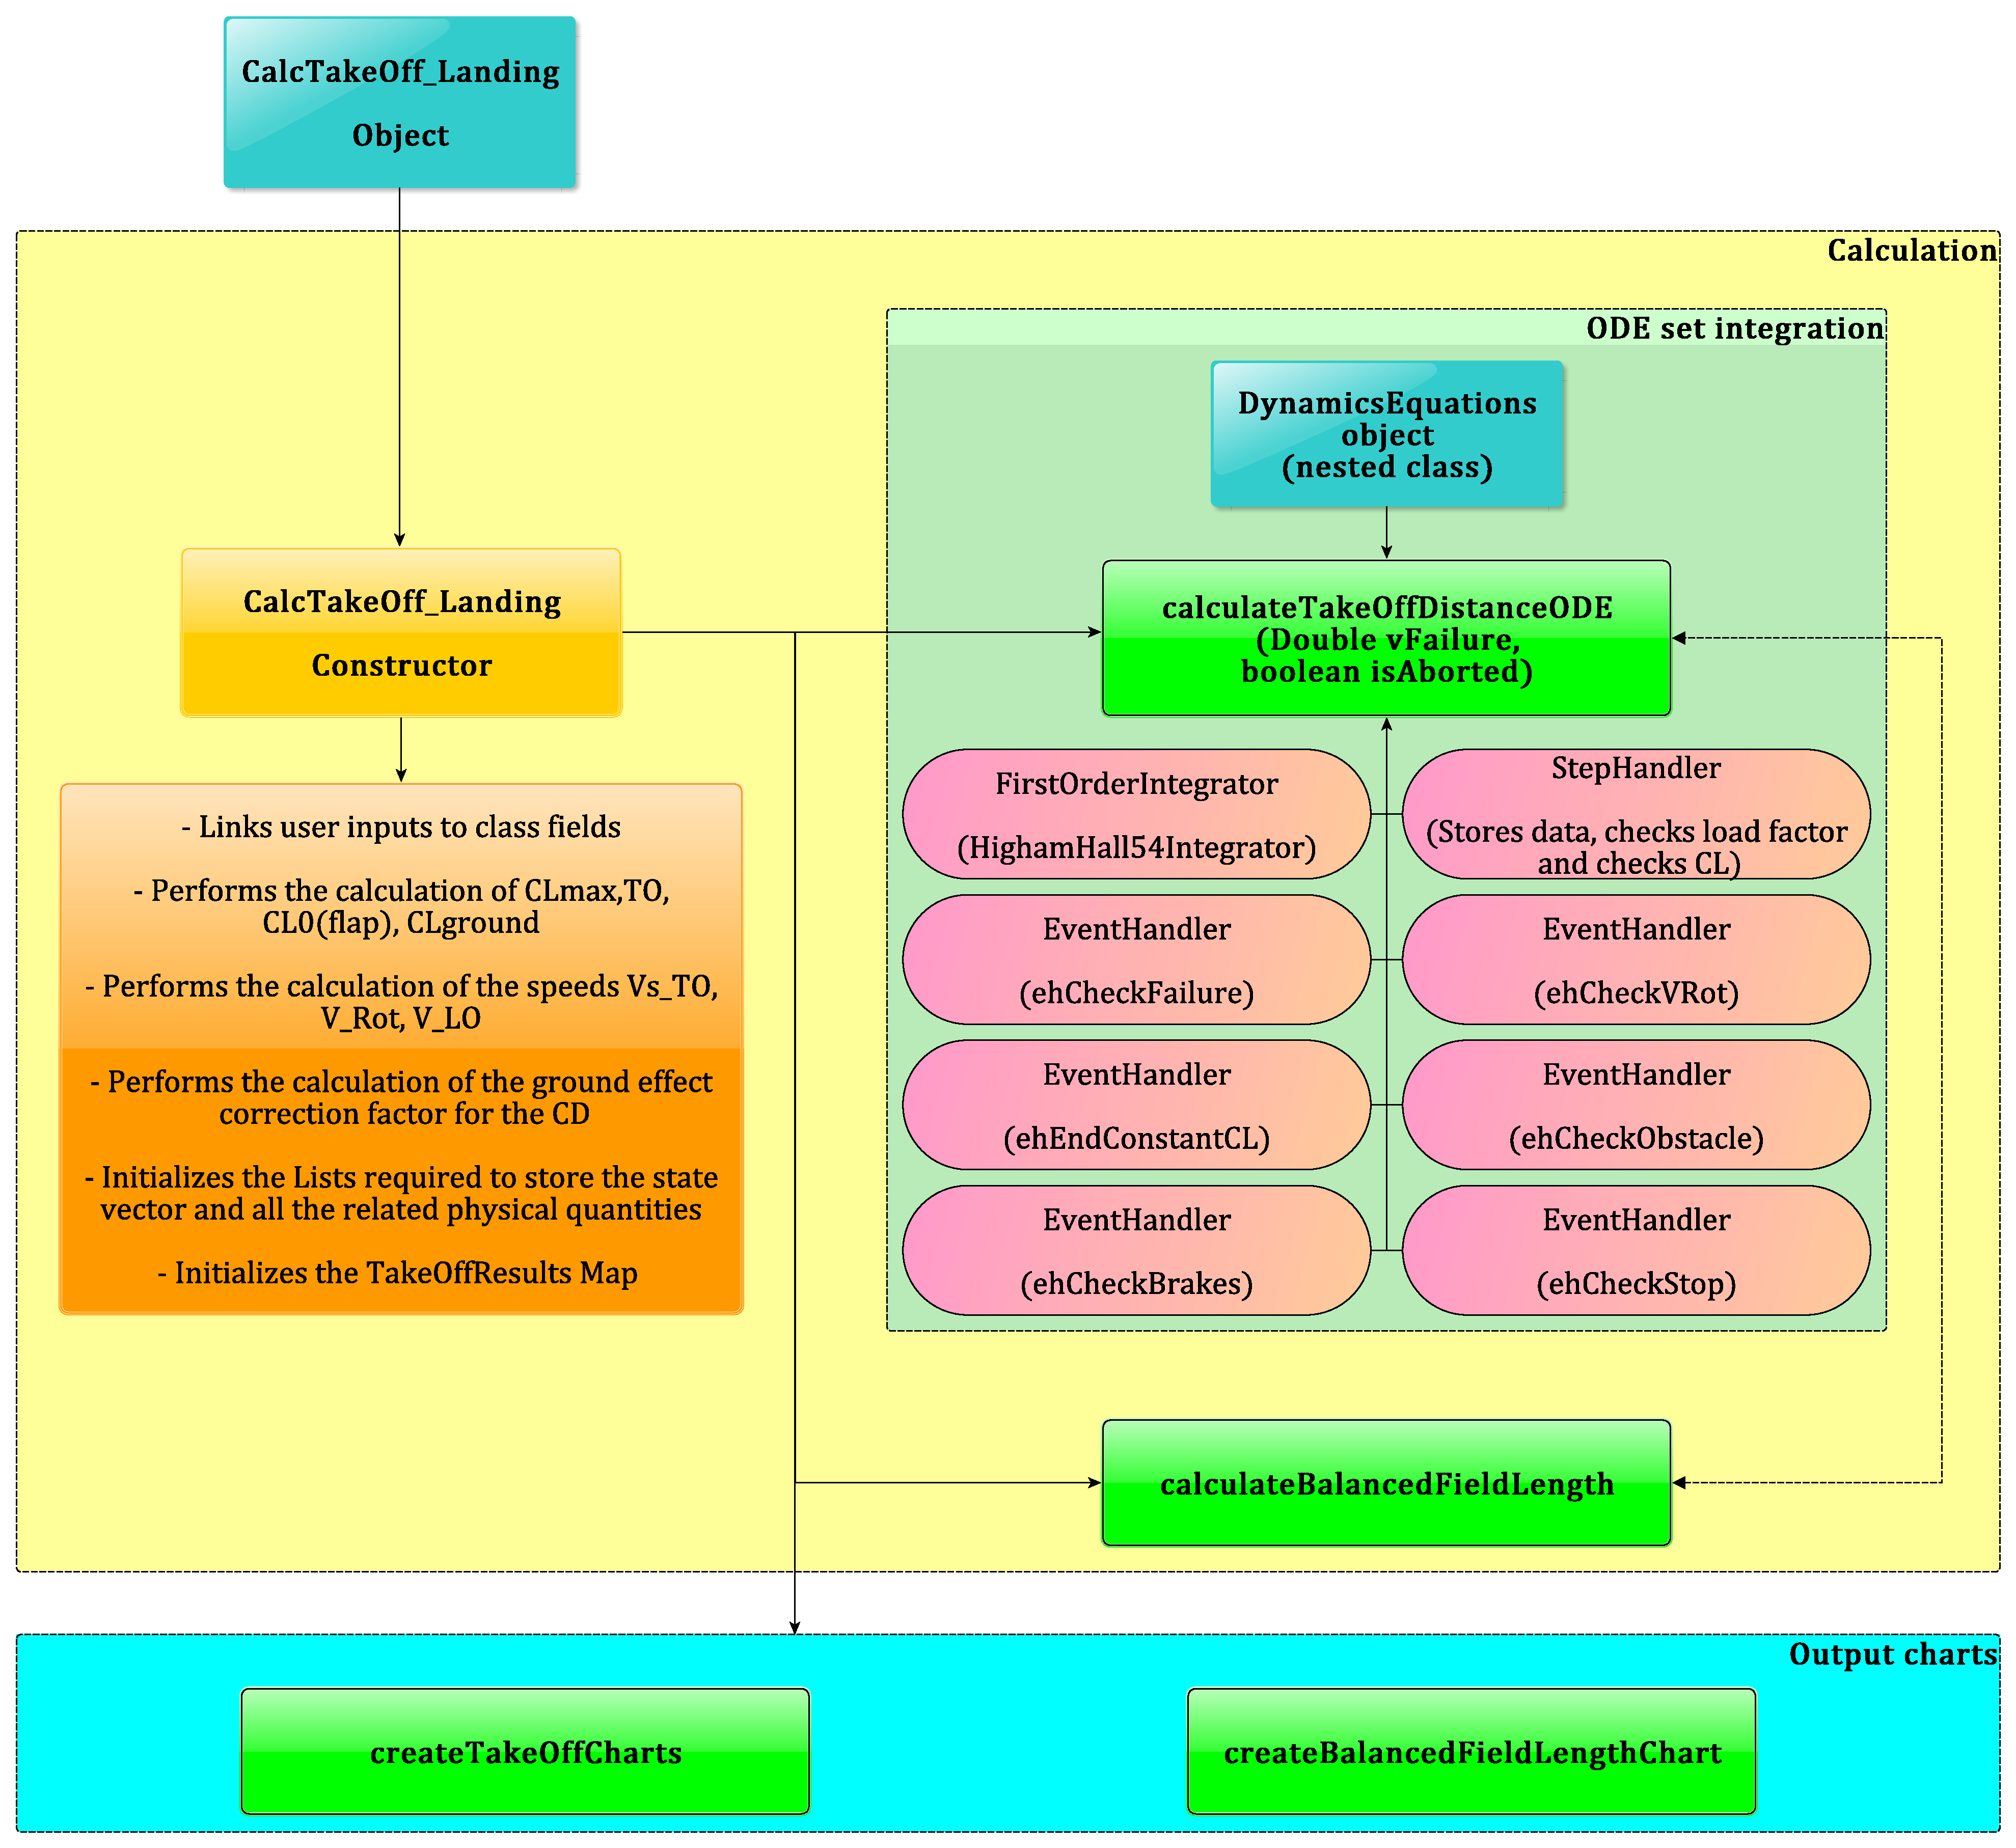
\includegraphics[keepaspectratio, width=\textwidth]{TakeOff_Flowchart}
\caption{\lstinline[language=Java]!CalcTakeOff! class flowchart}
\label{fig:CalcTakeOffFlowchart}
\end{figure}
%
%----------------------------------------- Landing ------------------------------------
\subsection{Landing}
The guideline followed for implementing the Java class in charge of the landing distance calculation is very similar to the one used in building the take-off class. The choice of having these two classes separated derives from the willing of not make the previous take-off class much complicated, since it's already full of flag and events necessary to manage the different possible situations.

\bigskip
\noindent
The class in exam is named~\lstinline[language=Java]!CalcLanding! and, similarly to~\lstinline[language=Java]!CalcTakeOff!, has a constructor in charge of performing all the preliminary operations such as linking all input data to the class fields, evaluate the high-lift devices effects on the wing and calculate the characteristics speeds during the landing phase. Since the class constructor is almost equal to the one in~\lstinline[language=Java]!CalcTakeOff! the reader can refer to previous paragraph for more detailed information.
%
\begin{table}[!t]
\makebox[\linewidth]{
\begin{tabular}{p{0.25\linewidth}p{0.7\linewidth}}
\toprule
\lstinline[language=Java]!aircraft! & An \lstinline[language=Java]!Aircraft! class object representing an aircraft parametric model \\ [0.2cm]
\lstinline[language=Java]!theConditons! & An \lstinline[language=Java]!OperatingConditions! object representing aircraft flight conditions \\  [0.2cm]
\lstinline[language=Java]!highLiftCalculator! & A \lstinline[language=Java]!CalcHighLiftDevices! object for managing flap and slat effects \\  [0.2cm]
\lstinline[language=Java]!kA! & Percentage of $V_s$ which defines the approach speed $V_A$ \\  [0.2cm]
\lstinline[language=Java]!kFlare! & Percentage of $V_s$ which defines the flare speed $V_{\text{Flare}}$\\  [0.2cm]
\lstinline[language=Java]!kTD! & Percentage of $V_s$ which defines the touchdown speed $V_{\text{TD}}$\\  [0.2cm]
\lstinline[language=Java]!mu! & The friction coefficient without brakes action \\ [0.2cm]
\lstinline[language=Java]!muBrake! & The friction coefficient with brakes activated \\ [0.2cm]
\lstinline[language=Java]!wingToGroundDistance! & The distance between the wing and the ground  \\ [0.2cm]
\lstinline[language=Java]!obstacle! & A given altitude value to overcome which defines the airborne phase ending \\ [0.2cm]
\lstinline[language=Java]!vWind! & The horizontal component of the wind speed, positive if opposite to the aircraft motion \\ [0.2cm]
\lstinline[language=Java]!alphaGround! & The angle of attack, in the \gls{ACRF}, of the wing when the aircraft is on the ground \\ [0.2cm]
\lstinline[language=Java]!iw! & The angle between the wing root chord and the \gls{ACRF} x-axis \\ [0.2cm]
\lstinline[language=Java]!thetaApproach! & The pitch angle during the approach phase (in $\si{\degree})$ \\ [0.2cm]
\lstinline[language=Java]!nFreeRoll! &  The number of seconds that characterize the free-roll phase\\ 
\bottomrule
\end{tabular}
}
\caption{\lstinline[language=Java]!CalcLanding! constructor input}
\label{table:CalcLandingInput}
\end{table}

\bigskip
\noindent
The first calculation method is~\lstinline[language=Java]!calculateAirborneDistance! which implements equations (\ref{eqn:Landing:Airborne:A}), (\ref{eqn:Landing:Airborne:B}) and (\ref{eqn:Landing:Airborne:C}) and populates the fields~\lstinline[language=Java]!sApproach! and~\lstinline[language=Java]!sFlare! with the calculated distances. Furthermore it begin to fill the~\lstinline[language=Java]!speed!,~\lstinline[language=Java]!landingDistance! and~\lstinline[language=Java]!verticalDistance! \gls{List}s in order to allow the plot of the trajectory and the speed during the whole landing phase.

\bigskip
\noindent
The second calculation method is~\lstinline[language=Java]!calculateGroundRollLandingODE!, which shares the same architecture of the method~\lstinline[language=Java]!calculateTakeOffDistanceODE! and accepts as input a~\lstinline[language=Java]!double! value, named~\lstinline[language=Java]!phiRev!, which represents the percentage of the thrust, calculated from the engine database, to be be used as reverse thrust in equation (\ref{eq:Take:Off:System:Dynamics:RHS:functions:B}). The~\lstinline[language=Java]!FirstOrderIntegrator! is still the~\lstinline[language=Java]!HighamHall54Integrator!, while the~\lstinline[language=Java]!FirstOrderDifferentialEquations! implementation is an instance of the nested class~\lstinline[language=Java]!DynamicsEquationsLanding! defined in the same way of the take-off class.

\bigskip
\noindent
In order to manage the only significant event, which is when the aircraft reaches a speed equal to zero, only one~\lstinline[language=Java]!EventHandler! has been implemented following the structure of \lstinline[language=Java]!ehCheckStop! defined for the aborted take-off run. Moreover all the physical quantities related to the ground run are stored in the related \gls{List}s at every integration step using the an instance of the \gls{Interface} \lstinline[language=Java]!StepHandler!.

\bigskip
\noindent
The peculiarity of this case, unlike the take-off, is that the integration starts from the end of the flare phase, with an initial position and a speed different from zero. This means that this method requires having previously carried out the calculation of the airborne distance, or having previously assigned values to~\lstinline[language=Java]!sApproach! and~\lstinline[language=Java]!sFlare!. 

\bigskip
\noindent
To allow the calculation of the total landing distance, without forcing the user to call each of the previous methods, these latter are enclosed inside a new method named ~\lstinline[language=Java]!calculateLandingDistance!. This choice derives both from the willing of simplify the usage of the class, both from the willing of preventing runtime errors in case the user wants to only calculate the distance to the ground without having assigned the values of the distances of the previous phase. The class is then completed by the method~\lstinline[language=Java]!createLandingCharts! which is in charge of creating the trajectory and speed charts, during the whole landing phase, along with the charts of all the physical quantities of interest during the ground run.
%
\begin{figure}[H]
\centering
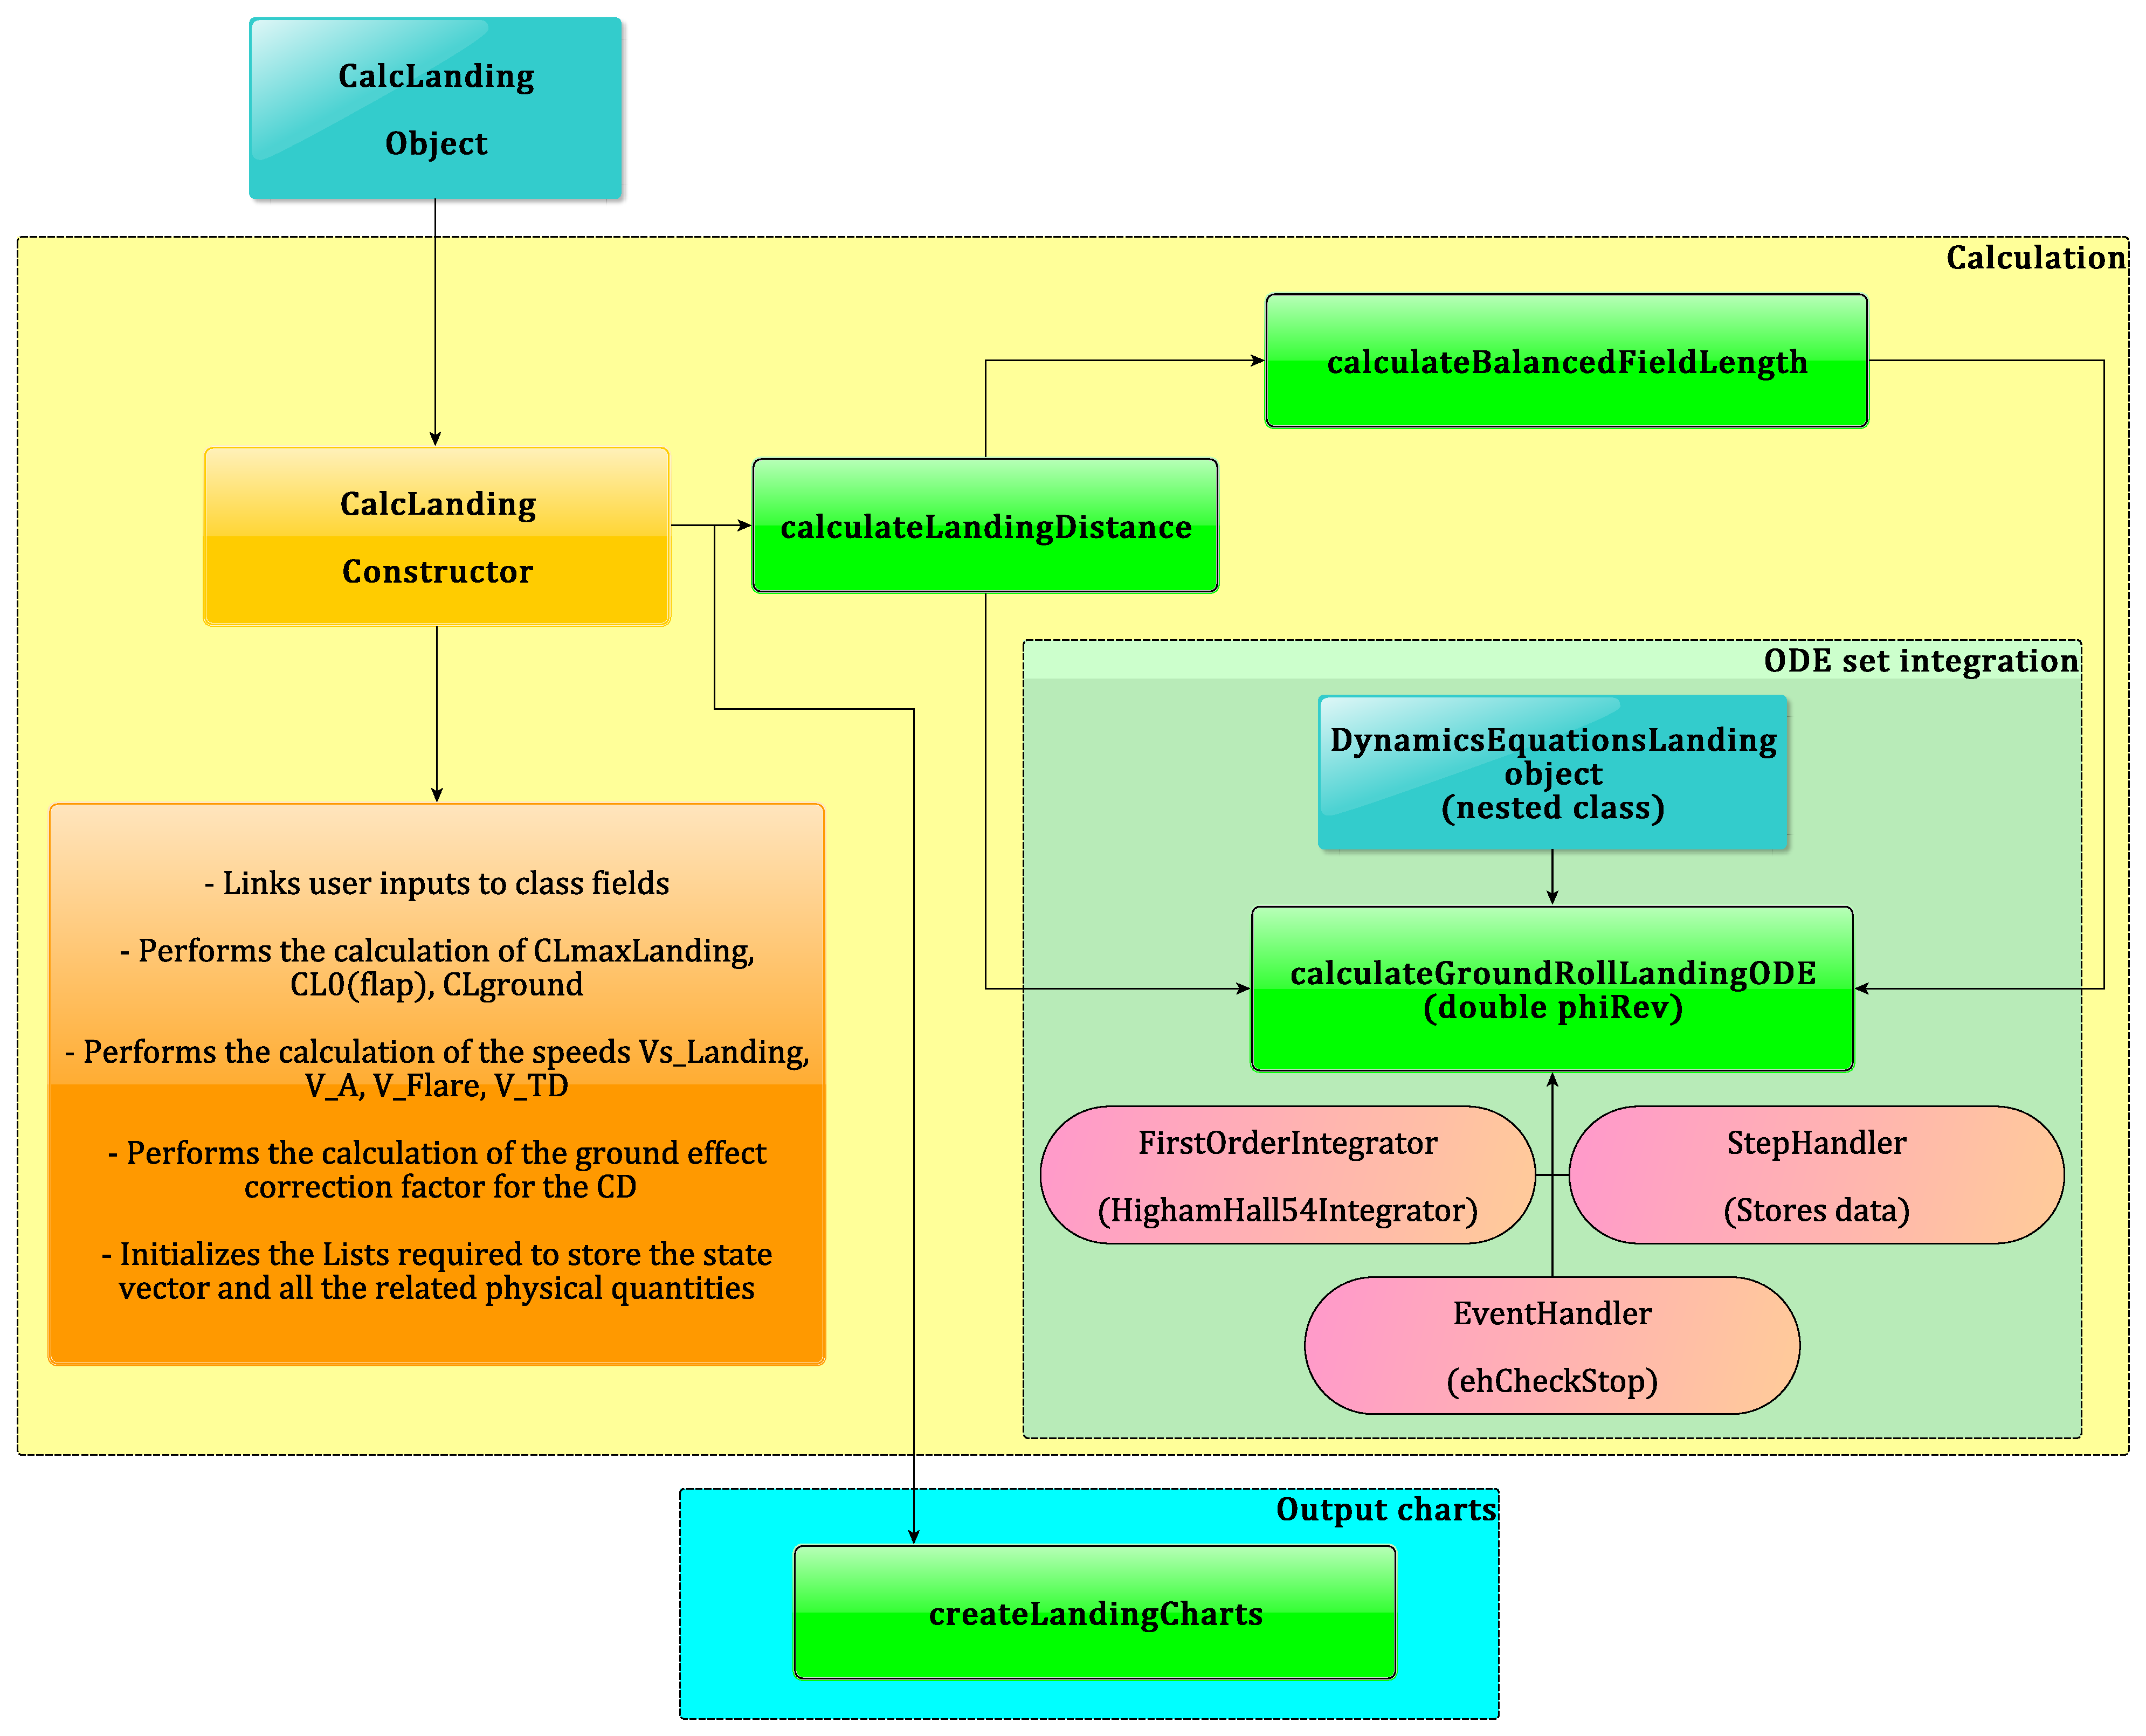
\includegraphics[keepaspectratio, width=\textwidth]{Landing_Flowchart}
\caption{\lstinline[language=Java]!CalcLanding! class flowchart}
\label{fig:CalcLandingFlowchart}
\end{figure}
%
%----------------------- CASE STUDY : ATR72 -------------------------
\section{Case study: ATR-72}
This paragraph has the aim of describing the Java class created to test the features implemented into \lstinline[language=Java]!CalcTakeOff! class and \lstinline[language=Java]!CalcLanding! classes; in particular a description of how to build these classes as well as a presentation, with comments, of the most important charts created, will be provided. 
%
Since the calculations are the same both for the B747-100B, both for the ATR-72, only the latter will be analyzed. 

\bigskip
\noindent
The first thing to do is to build the aircraft parametric model, and its analysis object, as described in paragraph \ref{par:DefaultAircraft}; then all information regarding high-lift devices have to be provided, in the same way of paragraph \ref{par:CaseStudyHighLift}, in order to allow the constructors of \lstinline[language=Java]!CalcTakeOff! and \lstinline[language=Java]!CalcLanding! classes to evaluate their effects (for the landing configuration the flaps deflection has been changed to \SI{35}{\degree} from the initial \SI{20}{\degree} related to the take-off). 
%
At this point all the preliminary steps are completed and it's possible to create \lstinline[language=Java]!CalcTakeOff! and \lstinline[language=Java]!CalcLanding! objects giving as input all data from tables \ref{table:CalcTakeOffInput} and \ref{table:CalcLandingInput}.

\bigskip
\begin{lstlisting}[caption={Input data and \lstinline!CalcTakeOff! object creation}, captionpos=b, tabsize=2]
	Amount<Duration> dtRot = Amount.valueOf(3, SI.SECOND);
		Amount<Duration> dtHold = Amount.valueOf(0.5, SI.SECOND);
		double mu = 0.03;
		double muBrake = 0.5;
		double kAlphaDot = 0.05; // [1/deg]
		double kcLMax = 0.85;
		double kRot = 1.05;
		double kLO = 1.13;
		double kFailure = 1.1;
		double phi = 1.0;
		double alphaReductionRate = -3; // [deg/s]
		Amount<Length> wingToGroundDistance = Amount.valueOf(4.0, SI.METER);
		Amount<Length> obstacle = Amount.valueOf(35, NonSI.FOOT).to(SI.METER);
		Amount<Velocity> vWind = Amount.valueOf(0.0, SI.METERS_PER_SECOND);
		Amount<Angle> alphaGround = Amount.valueOf(0.0, NonSI.DEGREE_ANGLE);
		Amount<Angle> iw = Amount.valueOf(1.5, NonSI.DEGREE_ANGLE);
//		PARAMETERS USED TO CONSIDER THE PARABOLIC DRAG POLAR CORRECTION AT HIGH CL
		double k1 = 0.0,  k2 = 0.0;

		CalcTakeOff theTakeOffCalculator = new CalcTakeOff(
				aircraft,
				theCondition,
				highLiftCalculator,
				dtRot,
				dtHold,
				kcLMax,
				kRot,
				kLO,
				kFailure,
				k1,
				k2,
				phi,
				kAlphaDot,
				alphaReductionRate,
				mu,
				muBrake,
				wingToGroundDistance,
				obstacle,
				vWind,
				alphaGround,
				iw
				);
\end{lstlisting}

\bigskip
\begin{lstlisting}[caption={Input data and \lstinline!CalcLanding! object creation}, captionpos=b, tabsize=2]
		double mu = 0.03;
		double muBrake = 0.5;
		double kA = 1.3; 
		double kFlare = 1.23;
		double kTD = 1.15;
		double phiRev = 0.25; // this takes into account of the reverse thrust
		Amount<Duration> nFreeRoll = Amount.valueOf(3, SI.SECOND);
		Amount<Length> wingToGroundDistance = Amount.valueOf(4.0, SI.METER);
		Amount<Length> obstacle = Amount.valueOf(50, NonSI.FOOT).to(SI.METER);
		Amount<Velocity> vWind = Amount.valueOf(0.0, SI.METERS_PER_SECOND);
		Amount<Angle> alphaGround = Amount.valueOf(0.0, NonSI.DEGREE_ANGLE);
		Amount<Angle> iw = Amount.valueOf(1.5, NonSI.DEGREE_ANGLE);
		Amount<Angle> thetaApproach = Amount.valueOf(4.0, NonSI.DEGREE_ANGLE);
		
		CalcLanding theLandingCalculator = new CalcLanding(
				aircraft,
				theCondition,
				highLiftCalculator,
				kA,
				kFlare,
				kTD,
				mu,
				muBrake,
				wingToGroundDistance,
				obstacle,
				vWind,
				alphaGround,
				iw,
				thetaApproach,
				nFreeRoll
				);
\end{lstlisting}
%
Now, regarding the take-off, if the user wants to perform a single calculation of the take-off distance, he can call the method \lstinline[language=Java]!calculateTakeOffDistanceODE!, specifying the condition he wants to analyze. The possible situations are resumed below, where \lstinline[language=Java]!vFailure! is an assigned \lstinline[language=Java]!Double! value.

\bigskip
\begin{lstlisting}[caption={Possible scenarios of calculation of the take-off distance}, captionpos=b, tabsize=2, label={lst:TakeOffScenarios}]
// AOE condition
theTakeOffLandingCalculator.calculateTakeOffDistanceODE(null, false); 
// OEI continued take-off
theTakeOffLandingCalculator.calculateTakeOffDistanceODE(vFailure, false); 
// OEI aborted take-off
theTakeOffLandingCalculator.calculateTakeOffDistanceODE(vFailure, true); 
\end{lstlisting}
%
Since this method provides only calculations, the user may want to generate charts regarding the evolution of the state vector and of the related physical quantities during the take-off run; in this case all it has to be done is call the method \lstinline[language=Java]!createTakeOffCharts! as shown below.

\bigskip
\begin{lstlisting}[caption={Take-off charts creation}, captionpos=b, tabsize=2]
// Generates all the output charts
theTakeOffLandingCalculator.createTakeOffCharts();
\end{lstlisting}
%
Following the flowchart of figure \ref{fig:CalcTakeOffFlowchart}, if the user wants, instead, to calculate the \emph{balanced field length}, and plot its chart, it's still very easy; in fact he has only to call the two methods \lstinline[language=Java]!calculateBalancedFieldLength! and \lstinline[language=Java]!createBalancedFieldLengthChart!.

\bigskip
\begin{lstlisting}[caption={Balanced field length calculation and plot}, captionpos=b, tabsize=2]
// Calculation of the balanced field length
theTakeOffLandingCalculator.calculateBalancedFieldLength();
// Plot of the balanced field length chart
theTakeOffLandingCalculator.createBalancedFieldLengthChart();
\end{lstlisting}
%
Regarding the landing, if the user wants to calculate the total landing distance, he has only to call for the method \lstinline[language=Java]!calculateLandingDistance!, giving as input the wanted \lstinline[language=Java]!phiRev!; this will then call the methods \lstinline[language=Java]!calculateAirborneDistance! and \lstinline[language=Java]!calculateGroundRollLandingODE! as described in the flowchart of figure \ref{fig:CalcLandingFlowchart}. Also in this case the previous call is used only to perform calculations so that, if the user wants to plot the results, the call that has to be made is to the method \lstinline[language=Java]!createLandingCharts!. The choice of separating the charts creation from the calculations derives from the willing of not to slow down these latter; in particular, because charts creation requires some time, a future iterative use of the calculation method will last longer if the method has to generate charts every time, with a negative effect upon a future optimization process.

\bigskip
\begin{lstlisting}[caption={Landing calculations and charts plot}, captionpos=b, tabsize=2]
// Calculation of the landing distance and its components
theLandingCalculator.calculateLandingDistance(phiRev);
// Results plot
theLandingCalculator.createLandingCharts();
\end{lstlisting}
%
In conclusion, the following pages show, firstly, a summary of take-off charts created in the three conditions of the listing \ref{lst:TakeOffScenarios} (by choosing a \lstinline[language=Java]!vFailure! of 30 $\si{\meter\per\second}$); after that, the output charts of the landing test will be reported in order to comment the main results. Instead, in the listings below, are resumed the main results of the take-off \gls{acr:AOE} condition (together with the results of the \emph{balanced field length} calculation) and of the landing analysis.

\bigskip
\begin{lstlisting}[caption={ATR-72 take-off test results}, captionpos=b, tabsize=2]
CLmaxTO = 2.1091586072792454
CL0 = 0.8590422136491769
CLground = 0.9961384471209911
VsTO = 52.9150212923735 m/s
VRot = 55.5607723569922 m/s
VLO = 58.2065234216109 m/s
-----------------------------------------------------------------
END OF GROUND ROLL PHASE
	switching function changes sign at t = 24.430078891752537
	x[0] = s = 733.8211736644284 m
	x[1] = V = 55.56077235699221 m/s
	x[2] = gamma = 0.0 deg
	x[3] = altitude = 0.0 m
	COLLECTING DATA AT THE END OF GROUND ROLL PHASE ...
---------------------------DONE!-------------------------------
		END OF ROTATION PHASE
	x[0] = s = 914.3532544050485 m
	x[1] = V = 60.489952274002775 m/s
	x[2] = gamma = 0.0 deg
	x[3] = altitude = 0.0 m
	t = 27.539416529357993 s
	COLLECTING DATA AT THE END OF ROTATION PHASE ...
---------------------------DONE!-------------------------------
		BEGIN BAR HOLDING
	CL = 1.7935218357497547
	Alpha Body = 8.725099918917621 deg
	t = 28.636788979040784 s
---------------------------DONE!-------------------------------
		END BAR HOLDING
	switching function changes sign at t = 29.13678897904078
---------------------------DONE!-------------------------------
		LOAD FACTOR = 1 IN CLIMB
	t = 30.376509808862576 s
---------------------------DONE!-------------------------------
		END OF AIRBORNE PHASE
	switching function changes sign at t = 31.67335982642885
	x[0] = s = 1174.0481557092937 m
	x[1] = V = 64.63429207083055 m/s
	x[2] = gamma = 3.6602788184585298 deg
	x[3] = altitude = 10.668000000000085 m
	COLLECTING DATA AT THE END OF AIRBORNE PHASE ...
---------------------------DONE!-------------------------------
BALANCED FIELD LENGTH = 1473.19533306467 m
Decision Speed (V1/VsTO) = 1.08720236687736 
---------------------------END!!--------------------------------
\end{lstlisting}

\bigskip
\begin{lstlisting}[caption={ATR-72 landing test results}, captionpos=b, tabsize=2]
CLmaxLanding = 2.670748822673163
CL0 = 1.2382555592182927
CLground = 1.3732629910434984
VsLanding = 45.1658739107583 m/s
V_Approach = 58.7156360839858 m/s
V_Flare = 55.5540249102327 m/s
V_TouchDown = 51.9407549973720 m/s
-----------------------------------------------------------------
		END OF THE LANDING GROUND ROLL
	switching function changes sign at t = 13.118579222455088
	x[0] = s = 688.5412017736963 m
	x[1] = V = -4.125172425872847E-15 m/s
---------------------------DONE!-------------------------------


------------------------RESULTS------------------------------
AIRBORNE DISTANCE = 163.126451534253 m
FLARE DISTANCE = 109.7652587941347 m
GROUND ROLL DISTANCE = 415.64949144531 m
TOTAL LANDING DISTANCE = 688.541201773696 m
-----------------------------------------------------------------
\end{lstlisting}
%
As can be seen the take-off distance required in \gls{acr:AOE} condition is about $\SI{1174}{\meter}$, at the maximum take-off mass of $\SI{22500}{\kilogram}$ and at sea level in standard atmospheric conditions, within a time of about $\SI{31.6}{\second}$; while the \emph{balanced field length} is bigger than the \gls{acr:AOE} take-off distance of about the 20\%. Moreover the \emph{decision speed} $V_1$ is bigger than the stalling speed $V_s$ as required by the \gls{FAR}-25 from table \ref{tab:Take:Off:Speeds:FAR25}. Comparing the \emph{FAR-25 take-off field lenght}, which is the 15\% bigger than the one calculated, with the take-off field length shown on the public brochure of the ATR 72-500, the two number are different of about the 4\%, validating, this way, the calculation made.  

\bigskip
\noindent
Regarding the landing test, the results obtained show that, at the maximum landing weight and at sea level in standard atmospheric conditions, the calculated landing distance is around $\SI{689}{\meter}$ with a ground roll distance of about $\SI{416}{\meter}$ covered in about $\SI{13}{\second}$. Deriving the \emph{FAR-25 landing field length}, which is obtained dividing the distance calculated by 0.6, this results to be similar to the one proposed onto the ATR 72-500 brochure proving that the calculation method works; in particular, the difference between the two distances is around the 7\%.

\bigskip
\noindent
Finally, with reference to the landing charts at the end of the chapter (from figure \ref{fig:Landing1} to \ref{fig:LandingEnd}), the reader can easily recognize the effect of the reverse thrust upon the landing distance; in particular, in case of \lstinline[language=Java]!phiRev!=0.25, the deceleration is bigger so that the speed decreases faster making the total landing distance shorter (about the 12\%). It has also to be noted that during the air run, the speed is assumed to be constant during the approach phase for then decrease, with a linear trend, from the $V_A$ to the $V_{\text{TD}}$ during the flare phase. 
%
\begin{table}[H]
\makebox[\linewidth]{
\begin{tabular}{p{0.35\linewidth}p{0.19\linewidth}p{0.19\linewidth}p{0.19\textwidth}}
\toprule
\textbf{ } & \textbf{ATR-72} & \textbf{JPAD} & \textbf{Difference(\%)}\\
\midrule
\textbf{FAR-25 Take-Off field length @ ISA, SL, MTOW} & $\SI{1300}{\meter}$ & $\SI{1350}{\meter}$ & $\approx3.7$\%\\ [1.0cm]
\textbf{FAR-25 Landing field length @ ISA, SL, MTOW} & $\SI{1067}{\meter}$ & $\SI{1147}{\meter}$ & $\approx6.97$\%\\
\bottomrule
\end{tabular}
}
\caption{Method results comparison with known data}
\end{table}
%
\clearpage
%
%
%-------------------------------Take-Off Charts------------------------------------------
%
\begin{figure}[H]
\centering
\includegraphics[keepaspectratio, width=1.09\textwidth]{TakeOff_Trajectory_AOE}
\caption{Take-off trajectory in \gls{acr:AOE} condition - ATR-72}
\end{figure}
%
\begin{figure}[H]
\centering
\includegraphics[keepaspectratio, width=1.09\textwidth]{Altitude_evolution_AOE}
\caption{Altitude evolution in \gls{acr:AOE} condition - ATR-72}
\end{figure}
%
\begin{figure}[H]
\centering
\includegraphics[keepaspectratio, width=1.09\textwidth]{TakeOff_Trajectory_OEI}
\caption{Take-off trajectory in \gls{acr:OEI} condition - ATR-72}
\end{figure}
%
\begin{figure}[H]
\centering
\includegraphics[keepaspectratio, width=1.09\textwidth]{Altitude_evolution_OEI}
\caption{Altitude evolution in \gls{acr:OEI} condition - ATR-72}
\end{figure}
%
\begin{figure}[H]
\centering
\includegraphics[keepaspectratio, width=1.1\textwidth]{AngularVelocity_vs_GroundDistance_AOE}
\caption{Angular velocities v.s. ground distance in \gls{acr:AOE} condition - ATR-72}
\end{figure}
%
\begin{figure}[H]
\centering
\includegraphics[keepaspectratio, width=1.1\textwidth]{Angles_vs_GroundDistance_AOE}
\caption{Angles v.s. ground distance in \gls{acr:AOE} condition - ATR-72}
\end{figure}
%
\begin{figure}[H]
\centering
\includegraphics[keepaspectratio, width=1.1\textwidth]{CL_vs_GroundDistance_AOE}
\caption{$C_L$ v.s. ground distance in \gls{acr:AOE} condition - ATR-72}
\end{figure}
%
\begin{figure}[H]
\centering
\includegraphics[keepaspectratio, width=1.05\textwidth]{AngularVelocity_vs_GroundDistance_OEI}
\caption{Angular velocities v.s. ground distance in \gls{acr:OEI} condition - ATR-72}
\end{figure}
%
\begin{figure}[H]
\centering
\includegraphics[keepaspectratio, width=1.1\textwidth]{Angles_vs_GroundDistance_OEI}
\caption{Angles v.s. ground distance in \gls{acr:OEI} condition - ATR-72}
\end{figure}
%
\begin{figure}[H]
\centering
\includegraphics[keepaspectratio, width=1.05\textwidth]{CL_vs_GroundDistance_OEI}
\caption{$C_L$ v.s. ground distance in \gls{acr:OEI} condition - ATR-72}
\end{figure}
%
\begin{figure}[!t]
\centering
\includegraphics[keepaspectratio, width=1.1\textwidth]{RateOfClimb_vs_GroundDistance_AOE}
\caption{Rate of climb in \gls{acr:AOE} condition - ATR-72}
\end{figure}
%
\begin{figure}[!b]
\centering
\includegraphics[keepaspectratio, width=1.07\textwidth]{RateOfClimb_vs_GroundDistance_OEI}
\caption{Rate of climb in \gls{acr:OEI} condition - ATR-72}
\end{figure}
%
\clearpage
%
\begin{figure}[H]
\centering
\includegraphics[keepaspectratio, width=1.07\textwidth]{LoadFactor_vs_GroundDistance_AOE}
\caption{Load factor in \gls{acr:AOE} condition - ATR-72}
\end{figure}
%
\begin{figure}[H]
\centering
\includegraphics[keepaspectratio, width=1.03\textwidth]{LoadFactor_vs_GroundDistance_OEI}
\caption{Load factor in \gls{acr:OEI} condition - ATR-72}
\end{figure}
%
\begin{figure}[H]
\centering
\includegraphics[keepaspectratio, width=1.03\textwidth]{LoadFactor_vs_GroundDistance_ABORTED}
\caption{Load factor in aborted take-off condition - ATR-72}
\end{figure}
%
\begin{figure}[H]
\centering
\includegraphics[keepaspectratio, width=1.06\textwidth]{VerticalForces_vs_GroundDistance_AOE}
\caption{Vertical forces in \gls{acr:AOE} condition - ATR-72}
\end{figure}
%
\begin{figure}[H]
\centering
\includegraphics[keepaspectratio, width=1.1\textwidth]{VerticalForces_vs_GroundDistance_OEI}
\caption{Vertical forces in \gls{acr:OEI} condition - ATR-72}
\end{figure}
%
\begin{figure}[H]
\centering
\includegraphics[keepaspectratio, width=1.06\textwidth]{VerticalForces_vs_GroundDistance_ABORTED}
\caption{Vertical forces in aborted take-off condition - ATR-72}
\end{figure}
%
\begin{figure}[H]
\centering
\includegraphics[keepaspectratio, width=1.1\textwidth]{HorizontalForces_vs_GroundDistance_AOE}
\caption{Horizontal forces in \gls{acr:AOE} condition - ATR-72}
\end{figure}
%
\begin{figure}[H]
\centering
\includegraphics[keepaspectratio, width=1.06\textwidth]{HorizontalForces_vs_GroundDistance_OEI}
\caption{Horizontal forces in \gls{acr:OEI} condition - ATR-72}
\end{figure}
%
\begin{figure}[H]
\centering
\includegraphics[keepaspectratio, width=1.06\textwidth]{HorizontalForces_vs_GroundDistance_ABORTED}
\caption{Horizontal forces in aborted take-off condition - ATR-72}
\end{figure}
%
\begin{figure}[H]
\centering
%Acceleration_vs_GroundDistance
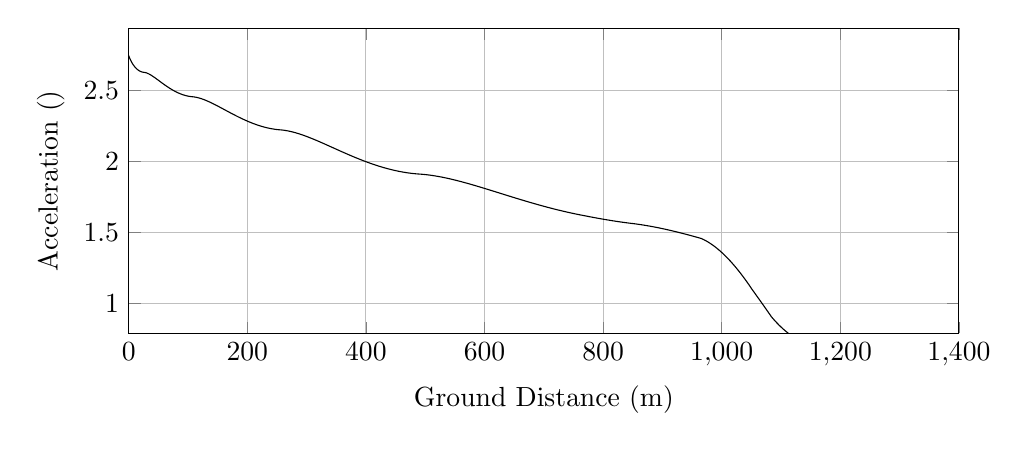
\begin{tikzpicture}

\begin{axis}[
width=\textwidth,
height=0.45\textwidth,
scaled ticks=false, tick label style={/pgf/number format/fixed},
xmin=0.0,
xmax=1400,
xlabel={Ground Distance (m)},
xmajorgrids,
ymin=0.7870546929072948,
ymax=2.9383329541999035,
ylabel={Acceleration ($\si{\meter\per\square\second}$)},
ymajorgrids
]

\addplot [
color=black,
solid
]
table[row sep=crcr]{
1.3729668748937997E-8	2.745933749634024\\
2.6049868369719035E-7	2.7459337463216693\\
2.0491224421327626E-6	2.7459337223163676\\
9.92442121137073E-6	2.74593361664894\\
4.7452367809869807E-5	2.7459331133935008\\
1.740064756114434E-4	2.74593141796994\\
4.0608377013922605E-4	2.7459283128250895\\
7.313431501337001E-4	2.745923966728787\\
0.0011549487327126044	2.7459183141309005\\
0.0016799013484208249	2.745911318665595\\
0.002295089346817705	2.7459031318683342\\
0.003009933382444524	2.745893631784023\\
0.003810608015426248	2.7458830054499908\\
0.004723484476856681	2.745870906509789\\
0.005727138856912631	2.7458576226878897\\
0.006836216967948795	2.7458429637322794\\
0.007997302399386296	2.7458276382144833\\
0.00929136979810952	2.745810580608766\\
0.010685558505459776	2.745792228663979\\
0.012178513621519987	2.745772603889116\\
0.013775244426719659	2.7457516442133327\\
0.015470070176169002	2.7457294279658626\\
0.0172374436815836	2.7457062929339147\\
0.019122918912604377	2.745681646264188\\
0.021104911040230538	2.7456557742244776\\
0.023190717999955576	2.7456285852738693\\
0.025355802981115103	2.7456004025085097\\
0.027620619195902148	2.7455709628304676\\
0.030020274690474198	2.7455398145480876\\
0.032476028269866286	2.7455079832228666\\
0.035054163466719815	2.745474612816359\\
0.037720846868992755	2.7454401452809734\\
0.04049779674511381	2.745404303593875\\
0.043329456594087365	2.745367807581193\\
0.04629652060163805	2.745329620662332\\
0.04934498934704602	2.745290442016606\\
0.052507657924119336	2.7452498537718295\\
0.055769483710642484	2.745208053078813\\
0.05917209570914676	2.7451645112972916\\
0.06264043916012321	2.7451201927906688\\
0.06620063977265622	2.745074766280724\\
0.06987962792775945	2.745027892179869\\
0.0736568184539585	2.744979836976057\\
0.07754284280095361	2.744930469346733\\
0.08151127871105612	2.744880128455919\\
0.08560324933017655	2.744828296550115\\
0.08985265585263943	2.7447745502252845\\
0.09413961367176535	2.7447204093860247\\
0.09857725310864562	2.744664448697618\\
0.10307959255469257	2.7446077566104368\\
0.10766008648593872	2.744550165853771\\
0.11234920964493048	2.744491296646081\\
0.11719267720457946	2.7444305805763873\\
0.12216973960582883	2.7443682839908865\\
0.12724007601918352	2.7443049160916244\\
0.13233299746505212	2.7442413617081813\\
0.13755256756750583	2.744176324555065\\
0.14287728588926696	2.744110077183268\\
0.1482946925752714	2.7440427783081276\\
0.15381585025670613	2.7439742941590106\\
0.15940564092189102	2.7439050633216198\\
0.16526271495916878	2.743832633069937\\
0.17120082448158402	2.743759314593124\\
0.17717889132867753	2.7436856165854584\\
0.18324322596131126	2.7436109697873574\\
0.189427022360885	2.7435349695339406\\
0.1957511558722988	2.743457364727397\\
0.2021484013779125	2.7433789844510024\\
0.20865863707071397	2.743299343476986\\
0.21548666343168166	2.7432159468507686\\
0.22220154781289658	2.743134061837388\\
0.22919671627301902	2.7430488935802986\\
0.23611678795738544	2.742964772871866\\
0.24306300975244904	2.7428804655838492\\
0.2503085190632165	2.7427926639555604\\
0.2576623280401219	2.74270369213178\\
0.26502430524173204	2.7426147629356477\\
0.2724963584449146	2.7425246467856903\\
0.2802001060647876	2.7424318847655185\\
0.2878583985474956	2.7423398174571867\\
0.2958320780323821	2.74224411264151\\
0.3040021452321372	2.7421462114990494\\
0.31208951788619	2.74204945948628\\
0.3202851396023423	2.7419515709453375\\
0.3287233234973125	2.7418509498073105\\
0.3370425959884752	2.7417519080250115\\
0.34575405233845447	2.7416483668644354\\
0.3545073625286812	2.7415445008529415\\
0.36338982075299686	2.74143927707345\\
0.37247557159370037	2.741331824878821\\
0.38151350442869847	2.741225116473271\\
0.3905554764834429	2.7411185361982797\\
0.3999457587520332	2.7410080342749286\\
0.4095398754587949	2.740895325049965\\
0.4189621792151833	2.7407848203234915\\
0.4285208811402964	2.7406729022160494\\
0.43828968955472236	2.7405587157868423\\
0.44807735398784176	2.740444501168418\\
0.45806002753764463	2.740328206966173\\
0.4682994371692033	2.740209125317234\\
0.4787752542918833	2.7400875051939693\\
0.4890770094685154	2.739968111629965\\
0.49985939134273727	2.739843363987376\\
0.5106597490205704	2.739718627718031\\
0.5213580865152188	2.739595283866114\\
0.532247733242454	2.739469951000051\\
0.5431365108549349	2.739344844457758\\
0.554075964429489	2.7392193713226414\\
0.5653450694020941	2.7390903409366887\\
0.5769901159382542	2.738957242270053\\
0.588512657344902	2.738825777773906\\
0.6004070039036553	2.7386903129467894\\
0.6121651247369502	2.738556638601956\\
0.6239717914322569	2.7384226491592862\\
0.6362472885961421	2.7382835883504875\\
0.6486428939173223	2.738143422272314\\
0.6610190736373547	2.7380037294208224\\
0.6737248046101814	2.7378605779440788\\
0.6862826225989949	2.7377193504710986\\
0.6991952542603428	2.7375743971928808\\
0.7122988072688032	2.737427572331951\\
0.7251463703465595	2.7372838790900627\\
0.7381769453061875	2.737138402838057\\
0.7516618647379176	2.7369881315120947\\
0.7654913705221527	2.736834310606014\\
0.7791756406994825	2.7366823919487455\\
0.7930637813125616	2.7365284991417216\\
0.8074774191984457	2.736369088689556\\
0.8215072375247947	2.7362142192435908\\
0.8361010597475598	2.736053431219534\\
0.8503303420601955	2.7358969585996338\\
0.8650627501899835	2.7357352618278403\\
0.8802332960144008	2.7355690814348668\\
0.8951742046771463	2.7354057362911055\\
0.9100334756324657	2.7352435957730297\\
0.9251067343345352	2.735079435666237\\
0.9403923630470314	2.7349132844243806\\
0.9559303815501943	2.7347447191307284\\
0.9712400158034169	2.7345789536451193\\
0.9869533781138684	2.7344091466658877\\
1.0029148609762486	2.734236997780573\\
1.0189962473881624	2.7340638988954913\\
1.035465185745812	2.733886982622522\\
1.0516742337458713	2.7337132054216866\\
1.067815735429615	2.7335404920408557\\
1.0846705971808022	2.7333605047019978\\
1.1012775250051634	2.7331835208984128\\
1.1180798406225687	2.7330048116164747\\
1.1351395900544134	2.7328237286921633\\
1.1526388687279154	2.73263835894707\\
1.1698922447507556	2.732455966615972\\
1.1875468452119025	2.732269712848928\\
1.2058383275300355	2.732077142510799\\
1.2239395537495579	2.731886975352393\\
1.2422020624207541	2.7316955142157697\\
1.2608769472440078	2.7315001426275947\\
1.2794948487006894	2.731305779649479\\
1.2979152553275424	2.7311138807814563\\
1.3166445915281573	2.73091917093961\\
1.3354141707340492	2.730724451882275\\
1.3543210821322504	2.730528719277727\\
1.373689361295591	2.73032863525778\\
1.3932049885015831	2.7301274608942405\\
1.4131781782225183	2.7299220154585475\\
1.4330139682345777	2.7297184263544425\\
1.4528243860883294	2.7295155352372795\\
1.4728783400745615	2.729310592226655\\
1.4934621752870565	2.729100693669997\\
1.5141408097620341	2.7288902940171758\\
1.53430654450827	2.7286855593626536\\
1.5553850389607948	2.728472025774905\\
1.5762653203499473	2.7282609685761434\\
1.5975496774716453	2.728046303569938\\
1.6196077215345106	2.7278243397435746\\
1.6413652536722467	2.727605899295412\\
1.663437310723463	2.7273848044555544\\
1.6860768385032747	2.727158548431424\\
1.7077101022266827	2.726942840558346\\
1.7297306410738114	2.7267237613893585\\
1.7520297891459062	2.7265024111794576\\
1.7743087535215367	2.7262817613558035\\
1.797257424336919	2.7260549980011213\\
1.8200802473615325	2.7258299974170024\\
1.8430350373473994	2.7256042147901303\\
1.8666926279964304	2.7253720605720746\\
1.8902808566018634	2.72514113040999\\
1.9138231309717848	2.7249111877288685\\
1.937187877956735	2.724683506686569\\
1.9611060682733261	2.724450973682445\\
1.9852138445648535	2.7242171481062742\\
2.009780393513653	2.723979437924413\\
2.0346228225622163	2.723739634761041\\
2.0593611988602687	2.7235014085153804\\
2.08477023517836	2.7232573149932806\\
2.110324766702745	2.7230124241566775\\
2.1352655781940433	2.722773991682768\\
2.160528860803022	2.7225330540312687\\
2.1862071157614817	2.722288750937233\\
2.2127756699400534	2.7220366021467237\\
2.2391904543957084	2.721786538650564\\
2.2653528664920257	2.721539475818613\\
2.292150575495974	2.7212870407551826\\
2.3187704640870406	2.721036905412479\\
2.3455495914188482	2.7207858982332622\\
2.372862901366455	2.7205305254301893\\
2.4007145172972395	2.7202707826704753\\
2.428100404243743	2.72001603228333\\
2.4555980306928005	2.7197608861757034\\
2.483374904362833	2.7195038000855876\\
2.511687733451976	2.7192424230947587\\
2.5402569276484597	2.7189793606402857\\
2.568415369317849	2.71872074613543\\
2.596987652715761	2.7184590025560453\\
2.6263861238451423	2.7181903927500546\\
2.655991481965028	2.717920608348247\\
2.6856115886357443	2.7176514041804687\\
2.7154221146045012	2.71738118698586\\
2.7455665152057707	2.7171086712897807\\
2.7752624694325894	2.7168409213882985\\
2.805457625653509	2.71656939071722\\
2.8358231840904597	2.716297056032584\\
2.8663460878589797	2.7160240421896784\\
2.897817297850832	2.7157433103512467\\
2.9287074004595235	2.7154685124985987\\
2.9603588456990284	2.715187708551693\\
2.9922321403815406	2.71490571640717\\
3.0241119471841866	2.71462444530067\\
3.056446055158509	2.7143399570513758\\
3.0889346922121366	2.7140549072190137\\
3.122221620829695	2.713763678408176\\
3.1546991615623394	2.7134803314856493\\
3.187635101478671	2.7131937884197734\\
3.221010117202278	2.7129042459478487\\
3.2543449374576605	2.712615872270808\\
3.288235920596943	2.7123235230382576\\
3.3223704322934555	2.7120299202652527\\
3.3562838593334394	2.7117390566035233\\
3.3906320903803255	2.7114453101597196\\
3.425633159699527	2.711146852210671\\
3.462387235801926	2.7108343880622456\\
3.4973980805087237	2.710537636483595\\
3.5324804241140235	2.710241147744873\\
3.5675385073174235	2.709945728382193\\
3.6040688981843845	2.709638816969628\\
3.6393612181513753	2.7093431890244997\\
3.6770856360342323	2.7090281416612143\\
3.7131729334920323	2.7087276833232927\\
3.749509707933214	2.7084260491268246\\
3.785733977879824	2.7081262444468592\\
3.8225309786916544	2.707822610564083\\
3.860867115351552	2.7075072478509306\\
3.89929745075254	2.7071921001654697\\
3.9373367205567504	2.706881130446619\\
3.9751626485832894	2.7065728578762025\\
4.013671158053867	2.7062599937888168\\
4.0521140617426425	2.7059486353631357\\
4.092377631210638	2.705623567578243\\
4.131586743753305	2.705308027124949\\
4.1715696979561425	2.7049872843873297\\
4.210522654700574	2.7046757949824176\\
4.250196810863292	2.704359538589963\\
4.2917015001093795	2.7040297652367293\\
4.332438976653355	2.7037071511860633\\
4.373124372895289	2.7033859958341147\\
4.414429464889761	2.703061013141131\\
4.455884944705147	2.7027359201134686\\
4.497250153511752	2.7024126010589393\\
4.537976875075978	2.7020953078843215\\
4.581399817640802	2.7017581350427298\\
4.623816269683994	2.701429893974078\\
4.666022338967499	2.7011043708260782\\
4.709098934189642	2.7007732491577343\\
4.752435367147649	2.7004412618628235\\
4.79531009100786	2.700113923220311\\
4.838191999420829	2.6997876304091646\\
4.881381760681686	2.6994601025113845\\
4.9256451804034285	2.6991255802428515\\
4.9704217340957495	2.6987883563581185\\
5.014356093293278	2.6984586198088563\\
5.058826350846283	2.698126010287651\\
5.104458009943745	2.697785910252903\\
5.149663211268795	2.697450177563721\\
5.194981168813841	2.6971147895925576\\
5.241194091283663	2.696773991377621\\
5.287987552078626	2.696430154327218\\
5.334426822383641	2.6960901499960244\\
5.380633359096258	2.6957530602096966\\
5.427524438012913	2.6954122052897027\\
5.476157635197664	2.6950599883398825\\
5.524667120325573	2.6947099813886997\\
5.5732739519824435	2.694360582160768\\
5.6208990292882195	2.6940195060851275\\
5.671502816366864	2.693658464116621\\
5.719824083529298	2.6933150154219874\\
5.767871110439133	2.6929747772519512\\
5.8169321963676754	2.6926286501345027\\
5.866076914057565	2.6922832358810025\\
5.917200682776528	2.691925289335387\\
5.96684810088939	2.6915790178532983\\
6.016885842403935	2.691231352228524\\
6.068639931677712	2.6908731577503717\\
6.119867755785197	2.6905199976544543\\
6.171030794930029	2.6901686602208663\\
6.222884713227881	2.6898139753337107\\
6.2735946138732235	2.6894684695538738\\
6.325883502103322	2.6891136013011465\\
6.379615386553551	2.6887504096481347\\
6.432194972482147	2.688396442468087\\
6.484528316464761	2.6880455368872473\\
6.536619297696934	2.68769764118571\\
6.589662958081361	2.687344796419861\\
6.644121795496577	2.6869840153423956\\
6.697445536614451	2.68663219810922\\
6.7518063163896365	2.686275003043974\\
6.8068829439682315	2.685914605406988\\
6.863205650636274	2.685547609679398\\
6.9185329265047315	2.685188625021353\\
6.974634519184049	2.684826152672259\\
7.031139830722298	2.6844626288388405\\
7.0870923879294985	2.6841041940757817\\
7.144766952910487	2.6837363176346836\\
7.2026451873548805	2.683368757231797\\
7.261191729679483	2.682998591553873\\
7.320502240843062	2.682625268876813\\
7.378210233177999	2.6822636424501294\\
7.437738452534925	2.6818922655745236\\
7.49714639104333	2.681523308417665\\
7.556502460410064	2.6811563316145213\\
7.617032771987237	2.680783794499826\\
7.676883327249088	2.6804171211405423\\
7.735740247984193	2.6800581575988813\\
7.796086087039788	2.679691776501249\\
7.856787102853412	2.6793249307229674\\
7.91721236259451	2.678961429481797\\
7.979013602666894	2.6785913752038963\\
8.039824025454376	2.6782289487607027\\
8.102419182184594	2.6778576340357727\\
8.16459313580776	2.6774905665511346\\
8.226347093952135	2.677127696565849\\
8.290527749984296	2.676752373844961\\
8.353592793320257	2.6763853613705777\\
8.417564177281012	2.67601487568339\\
8.482044607535009	2.675643270078857\\
8.547336806956285	2.6752688485572547\\
8.613293246319614	2.6748925126021685\\
8.6778048537894	2.6745262550450724\\
8.74454839911753	2.674149227258674\\
8.810708373588199	2.673777396453808\\
8.876548424968423	2.673409234250302\\
8.942828456712885	2.6730404887927257\\
9.010858044488913	2.6726639601609223\\
9.079453414959548	2.6722862922314583\\
9.148767802603732	2.6719066890561036\\
9.21609997183467	2.6715398811000908\\
9.285579683381485	2.67116336940079\\
9.355451712480097	2.670786767326205\\
9.423585014597279	2.670421494476032\\
9.493435356703696	2.6700490148237135\\
9.562655940911181	2.6696818813962357\\
9.63183713653898	2.669316926216502\\
9.703018708836247	2.6689434650398702\\
9.773178624863132	2.6685773872877823\\
9.844376937811855	2.6682079365263496\\
9.914998792594716	2.6678435040567887\\
9.98720270419701	2.6674729864037268\\
10.059478150570087	2.6671041981501142\\
10.132362020358627	2.6667344209387407\\
10.205876892438312	2.6663635857706476\\
10.279422251887688	2.6659947421935097\\
10.353305644514993	2.6656263553136483\\
10.42811398108589	2.6652555454284528\\
10.50332954727428	2.664884928557493\\
10.578207710262959	2.6645181680900603\\
10.65503529959097	2.6641441252244062\\
10.730232142651953	2.6637802356245537\\
10.805871937852555	2.6634164032193377\\
10.88265320376452	2.6630493287809767\\
10.958577899345514	2.6626885682826185\\
11.034861147941964	2.662328317504069\\
11.112742623646977	2.6619627989513033\\
11.190543636431041	2.661599949051814\\
11.267787598939979	2.6612419536263943\\
11.3462805052093	2.6608804641262784\\
11.423875697147409	2.6605253733666894\\
11.502735831556972	2.66016679186927\\
11.581465323066688	2.6598111062891867\\
11.661639233340708	2.6594512496614984\\
11.741743247575428	2.659094070532034\\
11.821864700430528	2.6587391681041073\\
11.901816327719768	2.6583873562373483\\
11.98361062800689	2.65802984404648\\
12.065425957085825	2.657674667049518\\
12.1478520915771	2.657319283720091\\
12.230956215923495	2.6569634524950505\\
12.313306905825911	2.6566132897052395\\
12.396632357805931	2.656261447402212\\
12.479578787946746	2.655913659143116\\
12.564327762802186	2.6555608318228234\\
12.648175874147956	2.655214251081233\\
12.736145481689512	2.6548532930755826\\
12.821080154398764	2.6545073614738826\\
12.908009536077355	2.6541559136608868\\
12.994986774303499	2.6538069029568296\\
13.081752199798046	2.6534613540348904\\
13.17035388279784	2.6531111740371047\\
13.257836697901475	2.652768065088189\\
13.34511613365563	2.652428366974772\\
13.433461823066896	2.6520871672573874\\
13.524108483575919	2.6517398400805456\\
13.611203924103116	2.6514087427638877\\
13.702229394080796	2.6510654420726993\\
13.792427706753081	2.650728010041674\\
13.882429934062493	2.6503940290968764\\
13.975435778888343	2.650051743756091\\
14.065832730112316	2.6497218173613817\\
14.157894546480026	2.649388598244756\\
14.250668806951023	2.649055631782466\\
14.343291987615704	2.6487260325270725\\
14.43744444968501	2.64839387373258\\
14.532636396723657	2.6480609912501123\\
14.625507232812737	2.6477390675021404\\
14.721503924398366	2.6474092478024884\\
14.818738382089133	2.6470782104461428\\
14.913572076739943	2.6467582780736505\\
15.009701633366973	2.6464369177531655\\
15.10815424447124	2.6461108524555685\\
15.206130868840724	2.6457894275225193\\
15.304035939715973	2.6454712794394446\\
15.403499839366233	2.645151168619309\\
15.503209871950865	2.6448333932172794\\
15.601718454553605	2.6445225108434887\\
15.700655560608023	2.6442133305209685\\
15.801250929860519	2.6439020954003567\\
15.899917805652187	2.643599879299895\\
16.001574124100856	2.6432916569963822\\
16.102638779863817	2.6429883870635598\\
16.204479333764816	2.6426859631921458\\
16.30489644092564	2.642390875444015\\
16.40578186591999	2.6420975095348966\\
16.509201471948074	2.641799986524223\\
16.614557195984908	2.6415002256988815\\
16.717657554831042	2.641210126302675\\
16.823039336622365	2.640916912552081\\
16.928576062495388	2.6406266046044653\\
17.03469945574068	2.640338038396731\\
17.140697318244236	2.640053160739731\\
17.246066414787876	2.639773277049187\\
17.35183930840021	2.639495622702711\\
17.458399953804133	2.639219234411631\\
17.565707112453843	2.6389442799060117\\
17.673103795073075	2.638672470550473\\
17.781888038667653	2.638400579402105\\
17.89115167195854	2.6381309531423165\\
18.00105710767307	2.63786323255278\\
18.110142905530395	2.6376009574466197\\
18.219697237410173	2.637341002414172\\
18.32752951944549	2.6370884953076636\\
18.43743745973078	2.6368345484445737\\
18.54904630654982	2.63658019384358\\
18.659302591714813	2.6363323952736817\\
18.770734536087716	2.636085450694776\\
18.883577445650936	2.635838949357387\\
18.996263390583444	2.635596364184675\\
19.108816920034535	2.635357616908477\\
19.22287647779894	2.6351192855805\\
19.33763586704334	2.6348831480062795\\
19.456324114791514	2.6346427711361047\\
19.57349394116079	2.634409291852097\\
19.690148252848566	2.634180600096859\\
19.80521137071168	2.633958691418372\\
19.92379170801214	2.633733794227746\\
20.04216631061405	2.6335131166802155\\
20.15848954929409	2.6332999786096893\\
20.278242138037896	2.6330843918964613\\
20.396206084226087	2.6328758170334643\\
20.516315546862906	2.632667302876359\\
20.637173924977112	2.632461401533406\\
20.75450010628387	2.6322652607421713\\
20.874378237858778	2.632068650375719\\
20.996035953832852	2.6318730325170687\\
21.11812959618858	2.6316806625120934\\
21.240471115580952	2.631491857446668\\
21.361479376438375	2.6313089928781865\\
21.485224699488654	2.631125973433857\\
21.607870280890317	2.6309485406063304\\
21.73242999733349	2.630772361329301\\
21.85704493170313	2.6306001480967662\\
21.98122016226351	2.6304325538620574\\
22.10826921766411	2.6302652125995127\\
22.235261614051304	2.6301021093246337\\
22.361664688868032	2.629943883831288\\
22.48780138980522	2.6297900776934346\\
22.614107216476143	2.6296401428980527\\
22.74409311379692	2.6294900871360998\\
22.873024137794893	2.6293454925824022\\
23.003512644166257	2.6292034414201826\\
23.132891545907036	2.629066846405708\\
23.26270690888247	2.628934029456868\\
23.39264146728729	2.6288053298831127\\
23.52277721573431	2.6286806696961964\\
23.654883767164463	2.6285584477188975\\
23.78569183677709	2.6284417091087624\\
23.917003007077597	2.628328794588147\\
24.047013652206026	2.628221204195908\\
24.178458227988493	2.6281166694027984\\
24.314609552493202	2.6280128759318746\\
24.447533097503474	2.627915932898171\\
24.579128452041708	2.627824218719879\\
24.71011994849615	2.627737123338611\\
24.843278471916108	2.627652868038229\\
24.975761222328053	2.6275733117861915\\
25.1115496753864	2.6274961796102385\\
25.247101122854083	2.627423621584068\\
25.384906965000688	2.627354391118195\\
25.522261036073317	2.6272899242628656\\
25.66123001648475	2.627229296090176\\
25.79865327455613	2.627173876444852\\
25.826335196219034	2.6271632574604533\\
25.839610403727477	2.62715822969495\\
25.841006316401874	2.627157703174394\\
25.84227013303559	2.6271572259940434\\
25.84770509053729	2.6271551682557828\\
25.86419328224909	2.627148869514051\\
25.90571916957557	2.627132632727095\\
25.999268866927544	2.62709410603191\\
26.123295978662824	2.627038901212371\\
26.250212562581652	2.6269775933396176\\
26.376891976518465	2.626911599588503\\
26.50638698165423	2.6268392423555404\\
26.634042370994827	2.6267631265942892\\
26.763333806613538	2.626681250837172\\
26.893207366259766	2.62659421847878\\
27.022905486492228	2.6265025738361114\\
27.153956322362554	2.626405232066988\\
27.287774297957696	2.626300978647955\\
27.42030033806219	2.6261929566003683\\
27.555504894698295	2.626077916748084\\
27.691130018821354	2.6259576762016144\\
27.82633313037239	2.6258330443348266\\
27.959508564917073	2.625705689812035\\
28.096515548835796	2.6255699768647354\\
28.232789703382153	2.6254303281033025\\
28.368684388406535	2.625286498680893\\
28.506541650227618	2.6251359904785243\\
28.64533374691623	2.624979841336361\\
28.78297783415192	2.624820465669056\\
28.92277775692753	2.6246540493487274\\
29.06227187463503	2.624483493060775\\
29.20212864139956	2.6243080372215513\\
29.34335827861657	2.624126392094661\\
29.483225747293005	2.623942134485322\\
29.625960812476485	2.623749682168036\\
29.76706561118049	2.6235551018597727\\
29.909402910999468	2.6233545237810842\\
30.051751399473822	2.623149671618658\\
30.196612335666572	2.6229368923312792\\
30.342192969749448	2.6227187353115538\\
30.48583400527584	2.6224992991267593\\
30.632658550781265	2.622270763203243\\
30.77846394498075	2.6220396350772806\\
30.92408133049836	2.6218047080288107\\
31.071091331299215	2.6215634400823893\\
31.218274793935116	2.6213178254024356\\
31.366705758252415	2.6210660719563164\\
31.515339333797037	2.6208099515408767\\
31.66356819769615	2.620550577189582\\
31.814689402684216	2.6202821391202162\\
31.96649953392354	2.6200084685109024\\
32.115424616034375	2.6197361526902787\\
32.266253234088566	2.619456531320976\\
32.41813832080348	2.6191711196609058\\
32.569791431087395	2.6188823653016966\\
32.722234201183724	2.618588359660447\\
32.876984607664	2.6182861188418736\\
33.031873994672836	2.6179798472058744\\
33.18502245018544	2.61767337730517\\
33.34135780547538	2.6173568541876238\\
33.49759920343199	2.6170368690402794\\
33.65385117142162	2.6167132684054444\\
33.8113313806527	2.6163835453824538\\
33.96985264489639	2.6160480723691215\\
34.126473036379195	2.6157131607910555\\
34.2857505660089	2.6153690959358693\\
34.4449212019973	2.6150218218705428\\
34.60566879064274	2.6146676745052684\\
34.76644486933921	2.614310071010496\\
34.92612701881755	2.613951597544056\\
35.08630421658309	2.6135887608266746\\
35.24825698849928	2.613218646437778\\
35.412303951281956	2.6128404656979436\\
35.57355277914179	2.612465573208352\\
35.73545353069308	2.612086065190393\\
35.89925038949356	2.6116990063305368\\
36.065161289279985	2.611303822719635\\
36.23047312008262	2.6109069894047563\\
36.39472205714358	2.6105097203642957\\
36.56135389445764	2.6101036997752756\\
36.72774532558607	2.609695316287241\\
36.89384825683493	2.6092847556652456\\
37.05904296416534	2.608873633171015\\
37.22702676294645	2.6084527521107095\\
37.39437475321985	2.6080306918927274\\
37.5621109943643	2.607604928234461\\
37.73270471709142	2.607169167240153\\
37.903359519601935	2.6067305347705387\\
38.071486842086316	2.6062957943756917\\
38.23815243703595	2.6058623319798837\\
38.40817787072022	2.6054176148453294\\
38.57751392140098	2.604972224462812\\
38.750215798728505	2.604515486819169\\
38.92001182640311	2.604064028086343\\
39.09310637700479	2.6036013939253158\\
39.26472366117933	2.603140360230884\\
39.436554723976656	2.6026764590104268\\
39.608961777617054	2.602208745072529\\
39.782828308010565	2.6017348303452126\\
39.956194359016465	2.6012600869258415\\
40.132391837044906	2.6007753954833523\\
40.30868053167249	2.6002882883371417\\
40.48611580488176	2.599795875967091\\
40.66383502946924	2.599300575623608\\
40.83999042132467	2.5988076076289266\\
41.018202681018664	2.598306879012876\\
41.19780999006247	2.59780023921822\\
41.37730467548502	2.5972919679986406\\
41.557010452813884	2.5967811949022925\\
41.73612816026986	2.5962702442991796\\
41.91555194917056	2.5957566162813004\\
42.09743589423803	2.5952341495078093\\
42.27807550146298	2.5947135135520316\\
42.45995188234755	2.594187603754664\\
42.6401410478328	2.593664926422731\\
42.822293873795985	2.5931349327029034\\
43.00585672428667	2.5925992336587598\\
43.189965171449515	2.592060371841985\\
43.372020236704074	2.5915260176090396\\
43.555636897252796	2.5909856106444664\\
43.74012033961118	2.5904412105939336\\
43.92429822300048	2.5898963139394615\\
44.106869824379004	2.5893548329369107\\
44.29411840239129	2.588798141810776\\
44.47920670866131	2.5882465834656143\\
44.665034305215386	2.5876915745572395\\
44.85242224248053	2.5871306821366113\\
45.03948098831597	2.5865695920897522\\
45.22811764277584	2.586002614453135\\
45.41548629589063	2.5854383417605273\\
45.60322541388645	2.58487188864763\\
45.793007222766036	2.584298230300096\\
45.983742663331824	2.583720675421648\\
46.172643153142886	2.58314771556424\\
46.36421599110457	2.582565713945945\\
46.553512793459404	2.5819897407332553\\
46.745018895697555	2.5814061887802406\\
46.93606459490553	2.580823220829023\\
47.126948089509526	2.580239969889381\\
47.31881294044018	2.579652975509168\\
47.5110690178297	2.5790640736859434\\
47.705448624448266	2.5784679831468953\\
47.90005519882567	2.577870546429364\\
48.09288923506665	2.577277947636331\\
48.28732881729917	2.576679844114947\\
48.484002572746206	2.5760743233998253\\
48.68089030454945	2.575467633349363\\
48.87532723390382	2.57486803095897\\
49.07073736177763	2.5742649991859343\\
49.2672083392297	2.5736582972862303\\
49.46586249263092	2.5730444865995894\\
49.661880987188695	2.5724384938105347\\
49.85966148345089	2.5718267615262587\\
50.05808618672894	2.571212777407524\\
50.25785665917266	2.570594402569249\\
50.45743808511885	2.569976421527972\\
50.65573800086891	2.5693622538365988\\
50.85948768734909	2.5687310825359084\\
51.061243703011925	2.5681059980424292\\
51.26368286286315	2.567478743109982\\
51.46416466063809	2.566857533975103\\
51.66475943174029	2.5662359893110347\\
51.86588207153103	2.56561285677663\\
52.07444928962187	2.564966744465173\\
52.2824430085781	2.5643225310284814\\
52.48676525705545	2.5636898422625745\\
52.69531994892206	2.5630442386830037\\
52.90027076850366	2.562410012697458\\
53.108186167814935	2.5617668705752035\\
53.31165724918766	2.561137759462768\\
53.520024946679996	2.560493831718171\\
53.72688450142306	2.559854920280424\\
53.93707391647578	2.5592061198138465\\
54.14518573319289	2.5585641573342945\\
54.35125853722778	2.5579289322446064\\
54.56213447502874	2.5572793940255876\\
54.77598621923464	2.5566212311207\\
54.987629956235494	2.5559704324655836\\
55.19778857845695	2.5553247914147734\\
55.41030974885841	2.55467252202679\\
55.62390503323701	2.554017625167454\\
55.83671574169797	2.553365831759879\\
56.047071254351536	2.5527222723040826\\
56.26137331252919	2.5520673989185383\\
56.47512769358855	2.5514149930840677\\
56.69105800830218	2.55075678108659\\
56.90937011004422	2.5500921924420785\\
57.12736617899088	2.549429482767894\\
57.346833156368504	2.5487632574065238\\
57.56476609337061	2.5481026676419045\\
57.78230894703917	2.547444262133678\\
57.99943865551505	2.5467881336539273\\
58.21827465292657	2.5461279153126446\\
58.436085045729726	2.545471882108224\\
58.6577546799423	2.5448053710641405\\
58.87982836766625	2.544138832936956\\
59.10336118170943	2.5434691447546607\\
59.324182403931715	2.542808819305696\\
59.545440661451366	2.5421484495030766\\
59.768227251413464	2.5414848224466517\\
59.99077485409802	2.540823240966116\\
60.21631063559073	2.54015416369662\\
60.44006004384342	2.539491792913134\\
60.66502706168687	2.5388272572727564\\
60.89133011288284	2.5381602583073883\\
61.11585558357916	2.5374999948556693\\
61.3432655409558	2.5368327945800493\\
61.57186440401435	2.5361637002878803\\
61.79868765088207	2.535501408748763\\
62.025670725987	2.5348402770909786\\
62.254132946411545	2.5341765056009926\\
62.48290793247415	2.5335135279774255\\
62.713817944074236	2.5328461162466924\\
62.94484116346062	2.5321801651283318\\
63.17805109236767	2.5315097497788024\\
63.41124119062552	2.530841264404774\\
63.64505576847972	2.5301728944345925\\
63.87735201907903	2.5295107788661895\\
64.11169045660182	2.5288448001638137\\
64.34725756208485	2.52817733598523\\
64.58324360279937	2.527510726208688\\
64.81881329818131	2.5268473544899654\\
65.05563560606473	2.5261825559991893\\
65.29467812810154	2.5255136850947695\\
65.53178653633495	2.524852393698131\\
65.77046761369158	2.5241889200770515\\
66.01019347650049	2.523524791474693\\
66.25262920761091	2.52285547188822\\
66.49342175078831	2.522193018006006\\
66.73393309567928	2.5215336779391944\\
66.97718905970893	2.52086921586132\\
67.21919788222482	2.5202105803525665\\
67.46413738735515	2.519546449583455\\
67.70584739194695	2.518893544044623\\
67.95375887035246	2.5182264574902717\\
68.19817148521656	2.5175713561374016\\
68.44413350233111	2.5169147004876002\\
68.68984243621705	2.516261345089669\\
68.93951041285982	2.515600171501796\\
69.19023531750676	2.514938969433662\\
69.43956667494601	2.514284217583624\\
69.68998597860525	2.513629416130965\\
69.94098943220166	2.512975932155717\\
70.1928405184459	2.5123231255440013\\
70.44659484061637	2.511668329081634\\
70.69926103579675	2.5110192971929557\\
70.95414956377036	2.5103675673854084\\
71.21136313866151	2.5097129793716446\\
71.46778788208749	2.509063506597747\\
71.7247351381395	2.5084158438377147\\
71.98234155897126	2.507769689085089\\
72.24107377350035	2.5071239256193767\\
72.4986091150376	2.5064843695454924\\
72.75949164810788	2.505839797213234\\
73.02014691132015	2.505199119753618\\
73.28114866838587	2.504560949336046\\
73.54342372888959	2.503923071226774\\
73.80584407854005	2.5032882764078206\\
74.07231166191039	2.5026472290607487\\
74.3389341302921	2.5020093971959803\\
74.60521354141642	2.501375988177486\\
74.87280568706873	2.5007431028336446\\
75.1403821105715	2.5001139292433843\\
75.41145333671997	2.4994803046180856\\
75.68265298797411	2.4988501932497016\\
75.95075857762194	2.498231039158717\\
76.2241428819712	2.4976035721719434\\
76.4990100438061	2.496976668570306\\
76.77213586328236	2.4963576955699853\\
77.04724851790667	2.49573822862106\\
77.32330034006353	2.4951207098630084\\
77.59850473375684	2.4945091566067346\\
77.87773830129439	2.4938928219842715\\
78.1565255546137	2.4932816837060106\\
78.43842651648492	2.492668017346257\\
78.720833678605	2.4920576010425153\\
79.00101298089581	2.4914563231480757\\
79.28359351218376	2.4908542717934887\\
79.57011733099088	2.490248328576058\\
79.85418914588558	2.4896520718283295\\
80.13919871477489	2.4890583687052414\\
80.42568449319114	2.4884661731421938\\
80.71472498530085	2.487873370981382\\
81.006853148924	2.487279025102887\\
81.2951972638476	2.4866971170884167\\
81.58524575795963	2.486116537145639\\
81.87461709596036	2.4855420949920353\\
82.1711642895769	2.484958381559892\\
82.46716486408064	2.484380782761332\\
82.76422974563803	2.483806186216814\\
83.05801377197795	2.483242957146957\\
83.35853301954708	2.482671999870737\\
83.65664966506407	2.4821108049392793\\
83.95487262936624	2.481554606519677\\
84.25322789115987	2.4810033792257986\\
84.55664509033022	2.4804481694309706\\
84.8599544590121	2.4798985860092557\\
85.16499148084048	2.4793513638033664\\
85.47187188044902	2.478806409028219\\
85.77908321853027	2.4782664837735044\\
86.08675489504844	2.4777313991684684\\
86.39784539041122	2.4771961342162765\\
86.71051296037359	2.4766640142286205\\
87.02583358957506	2.4761333445033173\\
87.34037846285594	2.4756099658506825\\
87.65395388450591	2.4750941674588303\\
87.96687312379424	2.4745854039580317\\
88.28527441497255	2.474073850456792\\
88.6103524516937	2.4735579588692937\\
88.92871226770333	2.4730590021066936\\
89.25003295857354	2.472561715850354\\
89.57522243846881	2.472064913921284\\
89.90247582737899	2.4715715482953424\\
90.22602529632545	2.471090281458441\\
90.5494223037065	2.4706157304863785\\
90.87816525326718	2.470140000358535\\
91.20455861430293	2.4696743344984124\\
91.53817773235312	2.4692052383281\\
91.87076195087604	2.46874453523425\\
92.20124984301029	2.468293613714687\\
92.53140503523474	2.4678500072923946\\
92.86389705561814	2.467410207209607\\
93.19815266874983	2.46697511608851\\
93.53304529783748	2.4665462917878456\\
93.86737084100128	2.4661252936021194\\
94.20337949361911	2.4657093387407842\\
94.54065981474497	2.4652990463300517\\
94.87396787418089	2.4649007234996034\\
95.21684847579547	2.4644983797555815\\
95.55392648231228	2.4641101935898275\\
95.89232371872416	2.463727831543161\\
96.23051075783204	2.463353072193108\\
96.57164052232307	2.4629825255521096\\
96.90762523479154	2.4626249186321765\\
97.24755293575913	2.462270552927021\\
97.58790661409188	2.4619232523826478\\
97.92576087813703	2.461585947168559\\
98.26661027452474	2.4612531815923795\\
98.6051908024865	2.4609301321117414\\
98.94563962387357	2.4606128512157275\\
99.28665364663627	2.4603026475156407\\
99.63350087797645	2.4599949576702347\\
99.97685593767679	2.4596981466115277\\
100.31593955776762	2.4594126383431973\\
100.65572384630482	2.4591341387793317\\
100.99616871909686	2.4588627388350837\\
101.3402339503516	2.458596236175948\\
101.67973054404297	2.458340953841132\\
102.01657591573795	2.4580952179760907\\
102.35656456518868	2.457854829697289\\
102.6941824316649	2.457623725275984\\
103.03547296258705	2.457397823628013\\
103.37623032340073	2.457180026797986\\
103.71852978299776	2.456969054425172\\
104.05851119314701	2.4567672705298635\\
104.3949509202441	2.4565752126830196\\
104.7329053851843	2.456389936423986\\
105.07104272194636	2.456212240406991\\
105.40742307340048	2.456043101164078\\
105.74423560014887	2.4558813834138933\\
106.07955743077031	2.455727984822288\\
106.41623710643992	2.4555816081016255\\
106.75618472497374	2.455441591416804\\
107.0942647435474	2.4553101084432747\\
107.43151869252583	2.4551866717490167\\
107.44650965670576	2.4551813642403237\\
107.45815118347005	2.4551772531208176\\
107.46233674961977	2.4551757772689795\\
107.46535588765028	2.4551747132015054\\
107.46808502617694	2.4551737507643727\\
107.4836206108138	2.455168259670489\\
107.53176708907421	2.4551511079163477\\
107.68672244793561	2.455094531599669\\
107.97570433527497	2.4549834451948627\\
108.27744765146667	2.4548597682328195\\
108.5816623935838	2.4547272061477434\\
108.88557241638279	2.4545869610121596\\
109.19209959959528	2.45443767243568\\
109.50241879336687	2.4542786003150896\\
109.81066605766154	2.4541127633367736\\
110.12101503747155	2.453937994054648\\
110.43285681965125	2.4537545790192175\\
110.74725799716322	2.453561818956234\\
111.06462449033057	2.4533593397004765\\
111.38211128519615	2.453148923592198\\
111.70119562731901	2.4529296108117045\\
112.02298633508096	2.452700564309909\\
112.34320819983824	2.452464869014065\\
112.66812620709393	2.452217884637398\\
112.99302416686388	2.451963112159949\\
113.31966045518399	2.4516991968576756\\
113.64998129974768	2.451424459279832\\
113.97857627498675	2.451143416865058\\
114.31304608469316	2.450849510906499\\
114.64448318111735	2.4505505571921855\\
114.98093514978115	2.4502393175308965\\
115.31969924418831	2.4499181287839766\\
115.65790718621022	2.449589741128423\\
116.00063352526521	2.4492491841404753\\
116.34235083463872	2.448901923487149\\
116.68621873349733	2.448544803075687\\
117.03331062078092	2.4481766222286128\\
117.37910048629482	2.4478022122028253\\
117.72869476105836	2.447416056567934\\
118.08005947084649	2.447020315368726\\
118.43363644355449	2.44661445841039\\
118.79186464668504	2.446195562722882\\
119.14769212941735	2.4457719010897243\\
119.5036618261702	2.4453406161077478\\
119.86270697471275	2.444898151431988\\
120.22616362054572	2.4444427272159954\\
120.58991121293201	2.4439794620158324\\
120.95538130513773	2.443506572675182\\
121.3195355377388	2.4430280793612997\\
121.68590041554987	2.4425394226513815\\
122.05305648207542	2.442042507730611\\
122.42257239354896	2.4415352206266228\\
122.79503144936103	2.4410167087569397\\
123.16629137010841	2.4404927909789507\\
123.53950748252527	2.439959095724661\\
123.91239367862553	2.4394189483888704\\
124.29026003316017	2.4388646308631676\\
124.66301933937496	2.438311045841078\\
125.03890311735066	2.4377461242287524\\
125.41380975776434	2.4371760734767376\\
125.7896808967325	2.4365980418067945\\
126.16837244152023	2.4360091772577572\\
126.54595968852882	2.4354156387065453\\
126.92471834906405	2.434813947054397\\
127.30294276405039	2.4342068948637348\\
127.68255852126984	2.433591469128208\\
128.06243727540487	2.4329695571547303\\
128.44360431740483	2.432339541404442\\
128.82265748788262	2.4317071612453454\\
129.1989690567886	2.4310736703116387\\
129.57765386613931	2.4304305602421765\\
129.95508099647026	2.429784065084977\\
130.33359114840187	2.4291302715149827\\
130.71373745886524	2.4284682576146626\\
131.09453904397424	2.4277997749107643\\
131.47657586018488	2.4271238577704235\\
131.85678563989967	2.426446027201812\\
132.23856625352113	2.42576032125654\\
132.61595336405918	2.4250775964184523\\
132.99976263915818	2.4243783357290276\\
133.38083522978053	2.423679242984316\\
133.76098428781995	2.4229771481541835\\
134.1363519425165	2.4222793654313444\\
134.51557915495124	2.421569932295995\\
134.8968696170101	2.4208521881638854\\
135.27419431482667	2.420137597883574\\
135.65215477207505	2.4194175854598914\\
136.03329358991255	2.4186873250908105\\
136.41192880753374	2.4179577730609862\\
136.7898079310749	2.417225694571063\\
137.17001317148595	2.4164851729427035\\
137.54844558779996	2.415744261492118\\
137.92617219433072	2.4150009862160164\\
138.30476964659732	2.4142523189260237\\
138.68390038934075	2.413498983015482\\
139.0631653430654	2.4127418378009757\\
139.4406106933401	2.41198488197385\\
139.81914660512416	2.4112223633220573\\
140.19767098864742	2.410456560906317\\
140.5730919292459	2.4096938425620706\\
140.95061983253072	2.4089237067743268\\
141.32838502869612	2.4081500093041033\\
141.70636515873298	2.4073728610224387\\
142.0839785067887	2.406593529688587\\
142.46357402350594	2.4058072184921997\\
142.84082211769783	2.40502296889394\\
143.21906727224075	2.4042339114596416\\
143.59963619096823	2.403437310882776\\
143.97984478872678	2.4026388326905357\\
144.35941603837455	2.4018391364099507\\
144.7355521893594	2.4010442230400466\\
145.11296635073694	2.4002442180265584\\
145.49073213867456	2.399441133914113\\
145.87033631970945	2.3986318541955978\\
146.24486520181193	2.397831210000894\\
146.6238757206513	2.3970188391759493\\
147.00096360401335	2.396208508945593\\
147.37874202190085	2.3953946757121454\\
147.756852900845	2.39457816388311\\
148.13572640408995	2.393758097000817\\
148.5136798644104	2.392938178662493\\
148.89083780486442	2.392118210713834\\
149.2712459042852	2.391289439886328\\
149.65303236723025	2.390455972301191\\
150.0329584616291	2.389624940771009\\
150.41363382646614	2.388790702960881\\
150.79322940570728	2.3879573271300165\\
151.17272478467066	2.3871227269328097\\
151.55400296227282	2.3862828087520374\\
151.93482601265913	2.385442551958211\\
152.31881414221942	2.3845940116132027\\
152.70208150063132	2.3837458190581575\\
153.08320649997165	2.382901190023449\\
153.4666285558243	2.382050340959543\\
153.84825937276264	2.381202396702336\\
154.23093781718723	2.380351107148919\\
154.61485031834388	2.379496102763693\\
155.00001234931443	2.3786373939872023\\
155.38285725409855	2.3777829898524283\\
155.7679513537659	2.3769227531344317\\
156.1509667875323	2.3760664034774726\\
156.53491934392343	2.3752072536116557\\
156.91995289130983	2.37434502792717\\
157.30625057946366	2.373479362158138\\
157.69121706207227	2.3726161237217385\\
158.07789765133754	2.371748534188164\\
158.46521012398495	2.3708790680405922\\
158.85138765236047	2.370011742814021\\
159.23964669847322	2.3691393833615075\\
159.62715395386465	2.368268403666744\\
160.01960115328984	2.367386056204964\\
160.4079207075476	2.366512776596168\\
160.79602490671402	2.36563981902208\\
161.18437278725975	2.364766199221803\\
161.57644284003254	2.363884138972799\\
161.96812230097612	2.363002938647095\\
162.35808768568592	2.362125623778489\\
162.75087300343483	2.3612420420191382\\
163.14546270495134	2.3603545272165904\\
163.53745675514648	2.3594730228399685\\
163.92955389373896	2.3585915050473067\\
164.32395276810763	2.357705079439211\\
164.71713266653478	2.3568217061873185\\
165.1102153740033	2.35593890902884\\
165.5035884424101	2.355055863096327\\
165.89816400198282	2.3541705682312966\\
166.29148626774366	2.3532885788431104\\
166.68861804276264	2.3523985917182593\\
167.082852347146	2.351515683455717\\
167.48006204110857	2.3506267458495653\\
167.8798182678497	2.349732796398407\\
168.27774435731556	2.3488436682392644\\
168.67741362640317	2.3479514207768712\\
169.07475368467374	2.3470651868695898\\
169.4759958044982	2.3461711163376826\\
169.87832784425882	2.3452755349517966\\
170.2792240364854	2.344384106753197\\
170.68126852540456	2.3434911272918937\\
171.08617821288442	2.3425928410644596\\
171.48766933901368	2.341703228415432\\
171.892744970828	2.340806814987485\\
172.29711201372032	2.339913155185136\\
172.70264003426053	2.339018160916506\\
173.1105289448074	2.3381192418897934\\
173.5163733808056	2.337226149563117\\
173.92577914808027	2.336326596791209\\
174.33607303977334	2.335426521117654\\
174.74614233406845	2.3345284082190787\\
175.15731444736514	2.3336293965914052\\
175.56901623635082	2.3327307892227083\\
175.97955109701695	2.3318363258755\\
176.39275298155184	2.330937702273025\\
176.80397138375372	2.3300450760546294\\
177.21946344336607	2.329144919042588\\
177.6332252263685	2.3282502942964154\\
178.05102033212842	2.3273487947563245\\
178.46725124888752	2.3264525543676644\\
178.88389799206544	2.325557341115923\\
179.29839533747668	2.324668693141324\\
179.71608569665375	2.3237752025766305\\
180.1342696339205	2.32288270874726\\
180.5538779958007	2.3219892775088473\\
180.97690569555635	2.321090736474277\\
181.39980810354632	2.3201946786391883\\
181.82328311928882	2.3192996671664883\\
182.24618807605736	2.3184081550362716\\
182.6731660166833	2.317510421204183\\
183.10035828358116	2.3166146524410083\\
183.5291445538124	2.315718009268359\\
183.95833265232255	2.3148230398976084\\
184.38634616388282	2.3139330622768055\\
184.8168339376561	2.31304053831765\\
185.24630581702252	2.3121527543741527\\
185.67754767955432	2.3112639955220837\\
186.109185775987	2.3103771499628856\\
186.53971883241212	2.3094953318031495\\
186.97132952004227	2.308614106272679\\
187.40711553434954	2.307727236429657\\
187.84220985117162	2.306844697971041\\
188.27778926256264	2.30596413782915\\
188.71822733349944	2.3050768055935897\\
189.16086434237673	2.304188169974439\\
189.6010380968554	2.303307624220924\\
190.03919041211265	2.3024342720484574\\
190.48016062316526	2.3015585113414065\\
190.92524363955386	2.3006778821099303\\
191.372330984798	2.2997966603754403\\
191.81766281185656	2.298922295360404\\
192.2649588892154	2.2980475215660183\\
192.7152080571317	2.29717049781034\\
193.16529614382966	2.2962973584252397\\
193.61551258619323	2.2954275767901127\\
194.0671041699889	2.2945587974042523\\
194.52074606224477	2.2936897982169953\\
194.9783774267325	2.2928169747246976\\
195.4358245305881	2.2919483704550094\\
195.89499401276925	2.2910804200107293\\
196.35432087192027	2.29021614095274\\
196.81831699949333	2.2893471419192934\\
197.28093205423113	2.288484832875148\\
197.74513845889334	2.2876237112361713\\
198.21238653581378	2.2867611842578457\\
198.6780372695403	2.2859058700391826\\
199.14562244096538	2.285051320833504\\
199.6172630308758	2.2841937787794144\\
200.085680559985	2.2833465240077064\\
200.55485539631252	2.2825023563416105\\
201.0284003638297	2.2816548831705905\\
201.5010163224531	2.2808136720525436\\
201.97949934275624	2.279966733779389\\
202.45676989461947	2.2791267029639997\\
202.93795341995116	2.278284633804679\\
203.42151825635358	2.27744333714352\\
203.9064451985618	2.276604678712552\\
204.39376498892221	2.2757669693589087\\
204.88144002832018	2.2749337898656847\\
205.3743097859811	2.2740969956561354\\
205.86751126322014	2.2732649672325973\\
206.36222180198536	2.2724357837290876\\
206.85620764580733	2.2716132370425086\\
207.35622660722595	2.270786197827218\\
207.85286701515986	2.2699703123930766\\
208.35554496397685	2.2691501921338437\\
208.85949164962352	2.2683337771305263\\
209.3606904933826	2.267527584023078\\
209.86430174661194	2.2667233414271317\\
210.37517113261447	2.2659135153305847\\
210.88826309775862	2.265106291807493\\
211.408532759536	2.2642940812050707\\
211.9275242572583	2.2634902283494576\\
212.45034341379437	2.2626869088461126\\
212.97278109853062	2.2618906907245666\\
213.5012611434281	2.2610919272299235\\
214.0307698600809	2.260298367573064\\
214.55632530210835	2.259517458773658\\
215.09027271075985	2.258730980013155\\
215.62992362610385	2.2579432040163745\\
216.17218538865313	2.2571588484810805\\
216.71273903148006	2.2563842166698143\\
217.25354139798316	2.2556165126472143\\
217.7992146693805	2.2548493165568644\\
218.34754045136725	2.254085939492425\\
218.89661223248612	2.2533291440783003\\
219.45761572436965	2.252563818122007\\
220.01811384548756	2.2518072106683293\\
220.5796054147944	2.251057348628902\\
221.1491613381006	2.2503050259601194\\
221.72392285119702	2.2495543519089907\\
222.29674345543788	2.248814773911077\\
222.87200016908895	2.2480806927809356\\
223.45476781204167	2.2473458994986784\\
224.04346163614804	2.246612743327802\\
224.62738211659592	2.2458946181678927\\
225.21466034383656	2.2451815330113867\\
225.80901970025303	2.2444692551194265\\
226.4067565685998	2.2437625152392293\\
227.010346212326	2.243058653573091\\
227.62015690700883	2.2423575809138097\\
228.23221085371028	2.2416641252690344\\
228.84135848872813	2.2409841492059526\\
229.46020606246555	2.2403037973268463\\
230.08791152904655	2.23962451579903\\
230.71342291791404	2.2389584838900456\\
231.3402722001092	2.2383019652353546\\
231.96207175272258	2.237661598553662\\
232.5840768980429	2.2370318898712833\\
233.21041275014744	2.2364088273333484\\
233.84076499381075	2.2357929904324703\\
234.4632722369638	2.2351959100520835\\
235.0951321894368	2.234601176398142\\
235.7164683430417	2.2340275104333625\\
236.33637872225546	2.2334662341004403\\
236.95807015301216	2.2329144958185676\\
237.57724458338066	2.2323761320972704\\
238.1954544769302	2.2318497405902384\\
238.81057478854058	2.2313370620076993\\
239.4264917144386	2.2308348356473227\\
240.0366097511752	2.2303483438025955\\
240.63918371105967	2.2298786569056217\\
241.24161561476188	2.229419836436943\\
241.8433627512665	2.2289723102569345\\
242.44272012201816	2.2285373001045503\\
243.03744426405035	2.228116281450559\\
243.6307298234035	2.227706865005068\\
244.22108413951537	2.227309998190906\\
244.8116939475828	2.2269235009469064\\
245.39744552343484	2.2265506298561997\\
245.97855029096053	2.2261910292632345\\
246.5589096408665	2.2258421732917872\\
247.13041662269836	2.2255087118698302\\
247.70663564674516	2.2251826514721484\\
248.28024698100222	2.2248682198189034\\
248.85288765982074	2.224564454598548\\
249.4193334510956	2.224273966746556\\
249.9777393310295	2.223997356302494\\
250.54131855768964	2.2237280307941525\\
251.10095479045611	2.223470406607258\\
251.65640742239583	2.223224408530201\\
252.20851363475686	2.2229894956588856\\
252.76218077146297	2.2227635597549096\\
253.31371341967355	2.2225481199438883\\
253.86551898536345	2.222342213140818\\
254.41422830739316	2.222147048359397\\
254.9572061395861	2.2219633575790283\\
255.0653176818724	2.2219279057873615\\
255.12993325322566	2.221906895339256\\
255.17825500251217	2.2218912701696016\\
255.20626764895485	2.2218822462499563\\
255.2307799315319	2.221874370500835\\
255.25350681352313	2.2218670855541918\\
255.27636741461964	2.2218597744009294\\
255.2901025823965	2.221855389728459\\
255.29493524708477	2.2218538483887693\\
255.30041476425401	2.2218521001387765\\
255.32542424174517	2.2218441047826696\\
255.431840924477	2.221809790194097\\
255.72188923316247	2.221713851752103\\
256.19571599032633	2.2215495739087965\\
256.67415123408614	2.2213742589191403\\
257.15505540016306	2.221188557634944\\
257.6368423781066	2.220993060856098\\
258.1230512066297	2.2207862547693775\\
258.61423458459376	2.220567707896195\\
259.1049940935744	2.2203397696000096\\
259.5982522152891	2.2201011037047182\\
260.09486806301686	2.2198512067286345\\
260.5959555145432	2.2195893748813527\\
261.1023053698689	2.219314998340587\\
261.6089919954627	2.2190306711996595\\
262.11906753970584	2.218734661689399\\
262.63243815947874	2.2184269215692023\\
263.14830217600297	2.218107856226906\\
263.66676080693014	2.217777349647611\\
264.1877265034735	2.2174354054872643\\
264.7128105393116	2.2170808727276556\\
265.241218472901	2.2167141732995255\\
265.7723922912836	2.216335620151221\\
266.3079016945154	2.2159439940722487\\
266.8503273810571	2.2155371935528327\\
267.3932272617866	2.2151199459981052\\
267.9365984091472	2.214692330831869\\
268.4918097049034	2.2142451659175686\\
269.04807221243857	2.2137868919753974\\
269.6097925731924	2.2133138095010647\\
270.17242368341533	2.212829684772851\\
270.7441513704771	2.2123273142660853\\
271.31667319188057	2.211813839181791\\
271.8922835348494	2.2112872141788866\\
272.47925332376417	2.21073960128831\\
273.06804504353704	2.210179665227172\\
273.66076346861166	2.2096053755286063\\
274.25294696226547	2.209021091006065\\
274.85204953299706	2.208419415799331\\
275.4590719216128	2.2077990829464973\\
276.0685465790958	2.2071655398666756\\
276.6808474128411	2.2065183952622025\\
277.29680014730513	2.2058567449011655\\
277.9224067517041	2.2051739367108585\\
278.5505103374435	2.204477611086179\\
279.17831818166474	2.2037709522184414\\
279.81790886718375	2.203040219253401\\
280.45539954927676	2.202301177006695\\
281.0966396233664	2.201547153524343\\
281.73735617862894	2.200783243215989\\
282.38112941523184	2.2000052659558564\\
283.0301801354616	2.1992104875794514\\
283.67721705328654	2.1984079099349207\\
284.3202688103162	2.1976002701437842\\
284.9599564878264	2.1967871053890056\\
285.60213884169843	2.1959611332978755\\
286.24205728342235	2.195128612826325\\
286.8783426797421	2.1942915966501397\\
287.5176726031193	2.193441453896205\\
288.14959414660166	2.1925923142210184\\
288.7790218355949	2.1917379149920313\\
289.41060269245395	2.1908720881422035\\
290.0373602432952	2.190004581853236\\
290.6616399781276	2.1891324221109327\\
291.28528823747513	2.1882532158649513\\
291.90747044142563	2.1873683040813363\\
292.5232553861292	2.186484968054768\\
293.13767407877424	2.185596251369275\\
293.74977203443143	2.184703716949506\\
294.36691018627903	2.1837967003650283\\
294.97422257673236	2.182897246316001\\
295.5803242078987	2.1819928935085953\\
296.18876641420377	2.1810784345812797\\
296.79141324013847	2.180166261540987\\
297.39276567122147	2.1792497807633247\\
297.9894421920609	2.178334342126881\\
298.5870928977196	2.1774114358177634\\
299.1813773675972	2.1764879005107254\\
299.77152323390305	2.1755651444500677\\
300.36612301275215	2.1746298256515306\\
300.9589816797394	2.1736917477653854\\
301.5517369040423	2.1727484415344804\\
302.13995783060716	2.1718071155806786\\
302.7265461416931	2.1708633010688203\\
303.31195316833305	2.1699163996118616\\
303.893632985354	2.16897068107039\\
304.47837522976045	2.1680152038285083\\
305.0603224805632	2.167059623470995\\
305.6386476191806	2.1661054611490913\\
306.2164211941447	2.165147784464958\\
306.79567265335925	2.1641833031163333\\
307.37231001650287	2.163218926340014\\
307.9484900815751	2.1622511631408274\\
308.52614124860884	2.161276845371755\\
309.10133925078446	2.1603026831998022\\
309.6811704644614	2.159316733523325\\
310.25396666777317	2.1583389407192453\\
310.82665929650705	2.1573576215107257\\
311.40151685857484	2.156368946462452\\
311.97010244433034	2.1553875407104144\\
312.53980750632184	2.154400769028112\\
313.10901660628747	2.153411498055127\\
313.67956238189845	2.152416609276753\\
314.2496933076443	2.151419222438893\\
314.8205968353319	2.1504173303654763\\
315.3893122304361	2.1494162128562335\\
315.9596108977621	2.1484093078225515\\
316.52927325433984	2.147400597921261\\
317.0962218845675	2.146393857614651\\
317.661512728229	2.145387313581532\\
318.22894706387933	2.1443742625039484\\
318.7945230010092	2.1433619149480556\\
319.36250947901885	2.142342693816164\\
319.92950718778627	2.1413227567225768\\
320.4959663753667	2.1403013705395244\\
321.0631721024022	2.1392762831596652\\
321.6290870613959	2.138251245534028\\
322.19457963905666	2.137224760081855\\
322.7618354565293	2.136192916341349\\
323.32829381843464	2.135160431012123\\
323.8944812959513	2.1341264139740925\\
324.4599775338005	2.133091701157084\\
325.0236279833782	2.1320584804222893\\
325.5930851369128	2.1310127668416543\\
326.1571709254106	2.129975146582318\\
326.723741026211	2.128931244309829\\
327.28922394543645	2.127887694887681\\
327.8556983549987	2.126840723202296\\
328.4233330667528	2.125790068469075\\
328.9893491077544	2.124740935922934\\
329.5546671193348	2.1236916871562777\\
330.1217964733877	2.122637719306182\\
330.68704439501266	2.1215859534914596\\
331.2526219304833	2.120532338558493\\
331.8212338226615	2.119471882534304\\
332.38563215932834	2.1184181631949706\\
332.9540373692553	2.1173558906467598\\
333.52282575474305	2.1162918813311666\\
334.0901133197508	2.115229718713011\\
334.6587212753741	2.1141641767917507\\
335.22495173293544	2.1131022427997204\\
335.79508811264384	2.1120321842685215\\
336.36651436910597	2.1109589553878356\\
336.93496842282195	2.10989061882366\\
337.5050159421993	2.10881865066278\\
338.07625180159437	2.107743862057567\\
338.64522733550257	2.106672796692953\\
339.21307292972244	2.105603383988063\\
339.78316525663524	2.1045293157173894\\
340.3517359250782	2.1034577426894865\\
340.92344762446896	2.1023799275904773\\
341.49725999120506	2.1012978793998096\\
342.0714758249467	2.10021484876724\\
342.6432180289123	2.099136314667774\\
343.2156727962654	2.098056318267221\\
343.788423593423	2.096975695534293\\
344.3632558179478	2.0958911279199244\\
344.936112850713	2.0948103191395964\\
345.5122282286983	2.0937234451068276\\
346.0894236551619	2.0926346660988067\\
346.6629357201275	2.091553015630354\\
347.2399030750438	2.0904650789951083\\
347.8149786266573	2.0893809881129126\\
348.3916437826483	2.0882942281274453\\
348.96682599762005	2.0872106372338015\\
349.5439461813521	2.0861238187564304\\
350.1219821225792	2.085035748253109\\
350.70068616715105	2.0839469410868414\\
351.28126445021985	2.08285517861776\\
351.8619451172309	2.08176384268437\\
352.4432281971418	2.0806720414159177\\
353.0222568578364	2.079585183944242\\
353.6045019024799	2.0784930492019047\\
354.18853493609936	2.0773983723820892\\
354.7725020489422	2.076304677843809\\
355.3555439607444	2.0752136181669885\\
355.94178228996793	2.074117531217567\\
356.52841816113096	2.0730217041561447\\
357.11491695053746	2.0719271813677196\\
357.7019804757698	2.0708326990263854\\
358.2889970677636	2.0697394433506195\\
358.8795343682166	2.0686408246670283\\
359.47011391270996	2.067543369430588\\
360.0611888887985	2.0664462813874236\\
360.65551621456757	2.0653445000252475\\
361.24837490254504	2.064246827243167\\
361.8399267049888	2.063152997230927\\
362.43366065279633	2.0620566048408673\\
363.0271841323796	2.0609621185456035\\
363.62092175430814	2.059868797986259\\
364.2172388023977	2.058772341330098\\
364.8170682790411	2.0576711007250967\\
365.4168935103936	2.0565715900035633\\
366.0167447450068	2.0554737963239846\\
366.613361119081	2.054383715029605\\
367.21449807554484	2.0532872236831823\\
367.81411987634317	2.0521953869396867\\
368.41428222027616	2.0511044981690754\\
369.0136835421291	2.0500169628099183\\
369.6184705538477	2.048921692318297\\
370.2203314850517	2.0478337923227743\\
370.8292817941207	2.0467352218957178\\
371.4325891230952	2.0456489986916795\\
372.03751184905457	2.0445620727425\\
372.64963462678804	2.0434644985000876\\
373.26236447571455	2.0423681821765456\\
373.87329119709466	2.041277469637664\\
374.48540637090855	2.040187056338617\\
375.0984288907292	2.039097495305686\\
375.71389401660815	2.0380061179418254\\
376.3292711349669	2.0369174658131852\\
376.94717931076855	2.035826960544064\\
377.56118057518813	2.0347459943042345\\
378.18357875745255	2.0336529744253005\\
378.80534455721454	2.0325638482233863\\
379.42657984220546	2.0314784686018923\\
380.05059226965216	2.0303911110355415\\
380.67279643790334	2.0293098110658017\\
381.29916382387717	2.0282242464375857\\
381.92611637580137	2.0271406908132175\\
382.55700718237256	2.0260534207709355\\
383.1838285741163	2.0249762739859998\\
383.815522641495	2.0238939285089517\\
384.4482555994399	2.022813036133588\\
385.0798113246169	2.0217374196047286\\
385.7142011583089	2.0206602979405197\\
386.35011647349825	2.0195839652444363\\
386.98806446889137	2.0185076293784476\\
387.62777316145673	2.01743181784932\\
388.2677779567189	2.0163590483054934\\
388.9088955203763	2.0152880011363115\\
389.5502219824099	2.0142202347706384\\
390.196085141905	2.0131486216095578\\
390.8411912635918	2.012082014883932\\
391.4850258768763	2.011021284452104\\
392.1348161747717	2.009954601807574\\
392.78657703059184	2.0088886169368267\\
393.43829425062995	2.007826678745676\\
394.0914803145356	2.00676637279003\\
394.74697534702034	2.0057064072787476\\
395.4022052560256	2.004651000539985\\
396.0614826489191	2.003593278798978\\
396.7253027860521	2.0025325671415235\\
397.389470201156	2.0014756542296404\\
398.0561080310739	2.0004192264167067\\
398.7226685692724	1.9993673818908313\\
399.391462726883	1.9983165326194312\\
400.06069563032156	1.9972695627023915\\
400.7298361745127	1.9962273430673902\\
401.4030004748297	1.9951835399156286\\
402.07673432903437	1.9941435938038579\\
402.7516637315023	1.9931065935099537\\
403.43308814587397	1.992064515589652\\
404.11621884098975	1.991024808921222\\
404.8017412836191	1.9899865121719458\\
405.4859375776791	1.9889553049878534\\
406.17916116612776	1.9879157062667154\\
406.869828889608	1.9868851969464423\\
407.5646978623407	1.9858537511018142\\
408.2605209917057	1.9848262851703216\\
408.95953036015305	1.983799588676332\\
409.6622694433204	1.9827729822263\\
410.36575705355096	1.9817509115960896\\
411.07335289700484	1.9807285915592856\\
411.7824393477108	1.979709909558284\\
412.49368167220496	1.9786939921741142\\
413.20637839560925	1.9776819235660077\\
413.9231120861825	1.976670142662917\\
414.64148448951505	1.9756621443134286\\
415.3640873105958	1.974654404724772\\
416.08758784728207	1.9736516756098457\\
416.8163237339112	1.9726480632908237\\
417.54818649211745	1.9716466199414198\\
418.2830458128634	1.9706476438998912\\
419.0197896011267	1.9696527511264574\\
419.7618468752946	1.9686574477069407\\
420.50810315351544	1.9676633982298468\\
421.2538226142991	1.9666770009394994\\
422.0024472585525	1.9656937752052972\\
422.7601619190325	1.964705807230772\\
423.51827295501266	1.9637246078995587\\
424.2791336478392	1.9627472169412767\\
425.04862066884436	1.9617662919432974\\
425.8175931526831	1.9607936457867101\\
426.59484428165274	1.9598183135035594\\
427.37319167714656	1.958849490553559\\
428.1560603980529	1.957883041042571\\
428.9441065434968	1.9569183463542998\\
429.73908511318723	1.9559534894529884\\
430.5390808738871	1.9549910265801893\\
431.34695313464147	1.9540277679043951\\
432.16146945503726	1.9530654629150561\\
432.97716762270886	1.9521107382210876\\
433.79906034498686	1.9511578944659411\\
434.63237437495366	1.9502012141583656\\
435.4690406415772	1.9492502593087764\\
436.31317920434697	1.948300581682909\\
437.1637869835322	1.9473536016709745\\
438.01645953609784	1.9464144223448097\\
438.8814827966934	1.9454720220169621\\
439.7524258551747	1.9445337885776426\\
440.63826385029256	1.9435904896584968\\
441.53868068573615	1.942643069567342\\
442.4384272900428	1.9417078939712207\\
443.3504012304777	1.9407718377002032\\
444.27758818218365	1.9398324331990464\\
445.208223124445	1.9389020323124977\\
446.1516186171384	1.9379717146054158\\
447.10189524137195	1.937047743675265\\
448.06481468075106	1.9361249889039414\\
449.03617443090013	1.9352079894896104\\
450.02512103574475	1.9342887399281925\\
451.0169824202726	1.9333813960883832\\
452.020591047557	1.9324782750407863\\
453.02360262247294	1.9315908066387548\\
454.0275908503903	1.930717678625125\\
455.03100385233165	1.9298603208522072\\
456.0319820328356	1.9290203239851524\\
457.02914229222506	1.9281987751211669\\
458.01937985050745	1.9273980545434086\\
458.99771244571184	1.9266218274260862\\
459.96197275276677	1.9258712880221664\\
460.92139296690334	1.9251388857975047\\
461.8616145847351	1.9244351036695493\\
462.80206306639445	1.923745036546007\\
463.7284486681126	1.9230789193900488\\
464.6393852721259	1.9224371548179335\\
465.54063936700334	1.9218151855932386\\
466.4349184101709	1.92121083349722\\
467.3198901301686	1.9206253734969052\\
468.20051759019884	1.9200552773907669\\
469.07226485074943	1.9195032459432606\\
469.9345383529743	1.9189693111954083\\
470.7902899889468	1.9184513519729718\\
471.6423737744856	1.9179474692301839\\
472.4877853124267	1.9174592646574875\\
473.3248054273006	1.9169874579343205\\
474.15679752822916	1.9165299145281485\\
474.98717382477696	1.9160846588943863\\
475.812191509144	1.9156535917157487\\
476.6363066147294	1.9152342927996107\\
477.44928852471696	1.914831756679289\\
478.25976263885	1.9144414692128522\\
479.0680268264706	1.9140632255614825\\
479.8720193908648	1.9136978928741777\\
480.6722055908582	1.9133451293208403\\
481.4638282544993	1.913006814641851\\
482.2537496794823	1.9126798413425705\\
483.0439784328089	1.91236338210116\\
483.8253492021597	1.912060966744796\\
484.60475037766423	1.9117697427594327\\
485.38148111107205	1.9114899097736364\\
486.15453177945005	1.9112217347233869\\
486.9234848636379	1.9109652368842638\\
487.6911837486889	1.9107193906062294\\
488.4532446281222	1.9104854915858627\\
489.2141943862101	1.9102620449202048\\
489.3656654782709	1.9102187750035968\\
489.9141839228952	1.910065445829419\\
489.9442198041063	1.9100572021480207\\
489.95165340794586	1.9100551640538526\\
489.95904841065203	1.9100531357634458\\
490.0087656528135	1.910039474305544\\
490.2229205115475	1.90998012937408\\
490.80762926712646	1.9098139882475396\\
491.5549224672211	1.9095929347788205\\
492.3059760305267	1.9093609860203213\\
493.05617311245896	1.9091195863122543\\
493.8124400481423	1.908866481685838\\
494.57147098753774	1.9086026844226072\\
495.33883357988543	1.9083261234890747\\
496.10451558660077	1.9080403583215273\\
496.8763216977479	1.9077424710640916\\
497.6516028092092	1.9074333817014901\\
498.43581565351974	1.9071107606051503\\
499.22198438592227	1.906777354176174\\
500.0155369982069	1.9064307685431618\\
500.8167457948026	1.9060706864337642\\
501.6207857715186	1.9056991664610488\\
502.43135952459795	1.905314411313884\\
503.2488031894138	1.9049161006374211\\
504.06841756255267	1.9045064478024192\\
504.89158107370974	1.9040847517667294\\
505.72576854379577	1.9036470074694045\\
506.5693448613787	1.903193790227991\\
507.4142887558387	1.9027293100792475\\
508.26842244805994	1.9022491739559726\\
509.12668782716764	1.9017560829115325\\
509.9922807952486	1.901248095939306\\
510.86952952987826	1.9007224315049953\\
511.75603474468153	1.9001802531132514\\
512.6525773610188	1.8996208422610983\\
513.552913573209	1.8990479584823463\\
514.4681532282782	1.8984543098294173\\
515.3867354533588	1.8978471839217366\\
516.3174024261396	1.8972206477495552\\
517.2602458293647	1.8965743256229226\\
518.213136886093	1.8959094045893212\\
519.1760409577637	1.8952256809005026\\
520.1413511846506	1.8945284724190263\\
521.1231004572105	1.8938074472060262\\
522.1209096033688	1.8930624424098643\\
523.1261067826763	1.8922996621561068\\
524.1419417493194	1.891516474462224\\
525.1629084556621	1.8907170041540406\\
526.1966720787225	1.889895095053141\\
527.232798559631	1.8890589432899638\\
528.2697748535691	1.8882098870890456\\
529.3125778912245	1.8873439090846054\\
530.3569535995234	1.8864645888042375\\
531.3923454146075	1.885581115383399\\
532.4241640074417	1.884689254648964\\
533.4600085213303	1.8837826000045483\\
534.4866261256011	1.8828730024093985\\
535.5020315541947	1.881962709030847\\
536.514508151736	1.8810446725778993\\
537.5229382799621	1.8801201675841668\\
538.5160648880578	1.879199952821573\\
539.5082343221115	1.8782711190202885\\
540.4856117025593	1.8773469828176474\\
541.4663647652112	1.87641066428179\\
542.4363165308484	1.8754759340879135\\
543.403649598117	1.8745352190464817\\
544.3586522503113	1.8735982871244108\\
545.3070641243951	1.8726598735668225\\
546.2506879020282	1.8717184576896524\\
547.1923729139526	1.8707713979186753\\
548.1284847870645	1.8698225559419757\\
549.0607273863563	1.868870430149943\\
549.9918578398997	1.867912374704844\\
550.9129328290753	1.866957827456614\\
551.8320704888101	1.8659986156921566\\
552.7431023110901	1.8650413901840208\\
553.6513866954954	1.8640807385303884\\
554.5567691623032	1.8631169834890065\\
555.4601447965442	1.8621493216093858\\
556.3560324901239	1.861183815872756\\
557.2510525453768	1.8602135088048848\\
558.144367784238	1.859239426861274\\
559.0395040047595	1.8582578181291471\\
559.9306875601039	1.8572751263220595\\
560.8184287789293	1.8562909470748803\\
561.6957839109712	1.8553131895245842\\
562.5803647812363	1.8543223419244375\\
563.4612104685039	1.8533307391837606\\
564.3388911147272	1.8523378832774222\\
565.215385530312	1.851341656273549\\
566.0886502219232	1.8503444998762033\\
566.9616941548127	1.8493430881350812\\
567.8301900811412	1.8483425026704507\\
568.6977679531799	1.8473386830883824\\
569.5620388889783	1.846334503702228\\
570.424462708284	1.845328383684881\\
571.2852292099337	1.8443202034233321\\
572.1493328191241	1.8433041782663846\\
573.0103554048726	1.8422879290286276\\
573.8681094542301	1.8412717944101846\\
574.7257926178972	1.840252082277571\\
575.584494453004	1.8392275648694643\\
576.4392320762051	1.8382042784217347\\
577.2895741354355	1.8371828618510078\\
578.1440860684359	1.8361530989219483\\
578.9955408132021	1.8351237626953472\\
579.8488294812946	1.8340890173119249\\
580.7009485845795	1.8330525707161498\\
581.5481034887393	1.832019140259142\\
582.398203180056	1.8309791566001463\\
583.2436286861621	1.8299420164024203\\
584.0951419205564	1.828894577142043\\
584.9447588199325	1.8278467056622891\\
585.7909961721582	1.826800322730227\\
586.6394553558484	1.8257485730329126\\
587.4827778011024	1.8247006559966725\\
588.3280079409788	1.823647896568175\\
589.1732196696316	1.8225927488882836\\
590.0172358784723	1.8215367505037592\\
590.860913103985	1.8204788984743092\\
591.7056349988741	1.8194175170465292\\
592.5455796206825	1.8183599971119087\\
593.390591992995	1.8172940033402503\\
594.23254291524	1.8162298437569269\\
595.0749775640184	1.8151631068321636\\
595.9164343501545	1.814095704448567\\
596.757445184641	1.8130270256013126\\
597.6003409863617	1.8119541623377766\\
598.4426744019354	1.8108802838332174\\
599.2847755368687	1.809805029594262\\
600.125707245069	1.808729657741857\\
600.9666449061319	1.8076527254284636\\
601.808765536209	1.8065727786307648\\
602.6493496090866	1.8054933619328994\\
603.4896653766809	1.8044129069784405\\
604.3324540913729	1.8033279391590065\\
605.1749627368547	1.8022420525508598\\
606.0172193894603	1.8011552669745674\\
606.8564954876942	1.8000711642392524\\
607.6995822420379	1.7989810242731283\\
608.5468271351888	1.7978844361091286\\
609.3853237539292	1.79679816627505\\
610.2285785394622	1.7957047772739938\\
611.0723962320026	1.7946097523919509\\
611.9144944458772	1.793516107544284\\
612.7572705739071	1.792420782603088\\
613.6039342512895	1.791319651499324\\
614.447700557992	1.7902215884581394\\
615.2875150228297	1.789128024779778\\
616.1283989744954	1.7880324752780012\\
616.9715554180159	1.7869334189518566\\
617.816851506552	1.785831074557084\\
618.6627080307358	1.7847275488640522\\
619.5079936234229	1.783624367262917\\
620.355287072993	1.7825182123625165\\
621.2019793580857	1.781412538268465\\
622.0488535053607	1.7803063712062164\\
622.9008554858297	1.7791932971659574\\
623.7470330382666	1.7780876726649844\\
624.5970610944692	1.7769769047447852\\
625.4445858106351	1.7758693432852386\\
626.2949117084559	1.7747581033970858\\
627.1456369954528	1.773646370702755\\
627.996202785663	1.7725349222351925\\
628.8493276316594	1.7714202525070197\\
629.7040179726459	1.7703037070548917\\
630.5541510983869	1.7691933293402333\\
631.4094242395336	1.7680764995969582\\
632.2635827644049	1.766961432544059\\
633.1201141992324	1.7658436214420772\\
633.9783198620232	1.764724025906065\\
634.8358449994842	1.7636057635854963\\
635.6949254776987	1.7624859642617348\\
636.5510277660717	1.76137058033426\\
637.4106283702604	1.7602512184024288\\
638.26983515646	1.7591329937321283\\
639.1281653037297	1.7580165767647982\\
639.9892853909298	1.756897243997511\\
640.854752101091	1.7557730243415293\\
641.7172955483825	1.7546534061914336\\
642.5803911560504	1.753533917760219\\
643.4447648773507	1.752413662665119\\
644.3076201978465	1.7512963070241243\\
645.1745276724305	1.7501746834561631\\
646.0402102676721	1.7490556660991494\\
646.9124608338768	1.7479292331382497\\
647.7810225029502	1.7468086773665923\\
648.6561125051048	1.7456808645688158\\
649.5284291267524	1.7445578317361687\\
650.3990692560633	1.7434381984962135\\
651.2710362166958	1.7423181425292729\\
652.1464633126748	1.7411949748188187\\
653.0220683418463	1.74007295522813\\
653.8956541670141	1.7389549349454159\\
654.7728777786044	1.737833718021482\\
655.6515481039796	1.736712157536986\\
656.5284362953553	1.7355944135411159\\
657.4113325495778	1.7344706069047673\\
658.2915193229558	1.7333518821120437\\
659.17716463588	1.7322279046106468\\
660.0651577261099	1.7311026840467463\\
660.9536046953733	1.7299786678144238\\
661.8402168340383	1.7288587862191362\\
662.7324470689205	1.727733676045954\\
663.6200112954277	1.7266163470779206\\
664.5127656227664	1.7254944318802576\\
665.4027074409514	1.724378033063548\\
666.2965782601134	1.7232587353863789\\
667.1908896376651	1.7221409597614152\\
668.084320193617	1.7210263937190131\\
668.985123002554	1.7199048022158925\\
669.8863392680419	1.7187849155529515\\
670.7862926077596	1.7176688511291633\\
671.6898074618846	1.7165506719391495\\
672.5888268774506	1.7154403823753164\\
673.4982782765783	1.714319607306411\\
674.4103925687491	1.7131980103360607\\
675.3150941849995	1.712087998569261\\
676.2268158638515	1.7109718990110894\\
677.1406213981061	1.7098558289580228\\
678.0557411892244	1.7087407793600207\\
678.9688521555179	1.7076308325314624\\
679.8873390970205	1.7065170627137594\\
680.8083547814929	1.7054029938429576\\
681.7306997118981	1.7042901304529794\\
682.6500311248872	1.703183740402348\\
683.5737488494256	1.7020749602459375\\
684.4960352365924	1.7009708224153632\\
685.4200123844039	1.699867625653504\\
686.3479632552264	1.69876270671213\\
687.2766127474456	1.6976600232389956\\
688.2061621748603	1.6965593790570344\\
689.1404800584801	1.6954562570822937\\
690.0764761874757	1.694354373653649\\
691.0152339372712	1.6932525113037675\\
691.9552419239503	1.6921524998716837\\
692.8950394637291	1.6910560887994528\\
693.8400111678282	1.689957057450783\\
694.7866818158914	1.6888595195885339\\
695.7347004483931	1.6877639334177896\\
696.6882574887352	1.686665529297878\\
697.6393666566034	1.685573558460721\\
698.5984440154043	1.6844761283542011\\
699.5498840703472	1.6833911315962968\\
700.5039755495234	1.6823068399444123\\
701.4647289348814	1.6812187842753383\\
702.4256797045559	1.6801343603427927\\
703.3874603974716	1.6790528942061602\\
704.3606354781252	1.6779626154470386\\
705.3315887422941	1.6768788694014836\\
706.3004122670179	1.6758015598360312\\
707.2768098841743	1.6747199643984945\\
708.2494358269255	1.6736467088741147\\
709.2282890376241	1.6725708091305207\\
710.2089151733701	1.6714972465270899\\
711.1951755925729	1.6704218760920493\\
712.1865307336975	1.6693453913559742\\
713.1761747054959	1.668275239069842\\
714.1673399979175	1.6672079559847899\\
715.1598728842257	1.6661437606954927\\
716.1583282218428	1.6650778532734902\\
717.1629472660959	1.6640100943452851\\
718.1700311785478	1.6629445100610822\\
719.1763338932042	1.6618845806777554\\
720.1876907614742	1.6608242243022313\\
721.201618282845	1.6597661338506482\\
722.2184418537404	1.658710043568684\\
723.235170191942	1.657659114463077\\
724.2594935927766	1.656605487350736\\
725.2822718646494	1.655558643060055\\
726.3107341130526	1.6545112475265258\\
727.3400446617545	1.653468309151676\\
728.3719103403353	1.6524281583444531\\
729.4113327961686	1.6513858662171454\\
730.4562931126598	1.6503435949894176\\
731.5065909482435	1.6493016659288253\\
732.5574458491262	1.6482649032926049\\
733.6186119363024	1.6472238073297722\\
734.676482187165	1.6461918199939674\\
735.7351170593906	1.645164993215896\\
736.800998200209	1.6441371415501762\\
737.8752235923619	1.6431073730628794\\
738.9508085948025	1.6420825012883684\\
740.030025186873	1.6410604393891606\\
741.1174055771332	1.6400370334056058\\
742.2130822925526	1.6390123397665604\\
743.3102570732492	1.637992839576305\\
744.4109860747094	1.6369767035883451\\
745.5166476604204	1.635962772477387\\
746.6263302357015	1.6349520004309106\\
747.7458154711032	1.633939285933022\\
748.8677740542141	1.6329314110242374\\
749.997151475181	1.6319240638363035\\
751.1325555959445	1.6309186521050458\\
752.2719517189332	1.629917111945916\\
753.4203420087897	1.6289152112661025\\
754.5711754188967	1.6279188163765936\\
755.7260036895639	1.6269266860442793\\
756.8938875174731	1.6259312465985127\\
758.065786260207	1.6249404167447605\\
759.247770693134	1.6239492488112464\\
760.4404154189538	1.6229575178659377\\
761.64317092529	1.6219659417111871\\
762.8455228703601	1.6209833335467456\\
764.0679862717263	1.6199931834370074\\
765.2987264665999	1.6190054314255176\\
766.4085307220014	1.618122605185865\\
766.5358897019526	1.618021772432912\\
767.7848317922183	1.617032332562915\\
769.0450472645446	1.6159889139824157\\
770.316931581486	1.6149401793569043\\
771.6083395962344	1.6138803466662388\\
772.9112380991485	1.612815359346611\\
774.2270303713512	1.6117448358850162\\
775.55388582573	1.610670280447533\\
776.893629267375	1.6095907082642067\\
778.2590064752919	1.6084970853761131\\
779.6390771149454	1.6073966733727612\\
781.0408632243589	1.6062856876674414\\
782.4719583829672	1.6051586963746298\\
783.9254029605222	1.6040203161454216\\
785.3937619636636	1.6028766217856978\\
786.8893778170732	1.6017204708413915\\
788.4179231510577	1.6005474649119344\\
789.9735980960556	1.5993614001533922\\
791.5542677978599	1.5981648450140975\\
793.1434824354058	1.5969688541241256\\
794.7563093028011	1.5957664471951687\\
796.3588663476394	1.5945767180309698\\
797.9570311300417	1.59340049795219\\
799.5313007987854	1.5922483965559024\\
801.0895110610122	1.5911183481194744\\
802.6055669418217	1.590023692664424\\
804.1018949910592	1.5889553241792918\\
805.5783591859272	1.5879096997123407\\
807.0307066077335	1.5868888576124087\\
808.4529908307093	1.5858962545394721\\
809.8505654906257	1.5849297137442324\\
811.2444364840742	1.5839774865008271\\
812.6158728333517	1.583045190017622\\
813.9667251199407	1.5821349211567752\\
815.3010783126617	1.5812441455323616\\
816.6204907399006	1.5803711882457216\\
817.9261081614768	1.5795150566753167\\
819.226186053904	1.5786716938587033\\
820.5043924755685	1.5778465992515383\\
821.7811573689405	1.5770339534413633\\
823.0442722941846	1.5762348138488305\\
824.2983674535399	1.5754495965544368\\
825.541081257411	1.5746781969850616\\
826.7810697424134	1.5739175842231958\\
828.0072700964611	1.5731701632623976\\
829.2275465246082	1.5724351973820898\\
830.440290401928	1.5717115069898706\\
831.6456016564753	1.5709993364655932\\
832.8458526198069	1.5702977616694724\\
834.037616834057	1.569607369556559\\
835.2234914579537	1.5689279924817385\\
836.3972899863502	1.5682609645004115\\
837.5756391031359	1.5676023673589023\\
838.7422917585684	1.5669533212286484\\
839.902452142522	1.566316040028656\\
841.0603218408189	1.5656879772009495\\
842.2105732200805	1.5650695918689888\\
843.3580616645866	1.5644608032549914\\
844.5012408269597	1.5638607919435965\\
845.6398059126466	1.5632699943883175\\
846.7724224635103	1.5626887764917803\\
847.8965100633054	1.5621180305202782\\
848.1209130838795	1.56176525060099\\
848.1623489143824	1.5616954216548957\\
848.2012937955549	1.5616751617081057\\
848.2388050923146	1.5616559138043122\\
848.2635941917742	1.561640041334969\\
848.2919709507985	1.56162673486309\\
848.4211104394196	1.561588744383148\\
848.9593804425128	1.561426197862195\\
850.1439050107567	1.5609927023697248\\
851.2989990610786	1.5603805609883143\\
852.4625415319017	1.559762153089793\\
853.6343291480857	1.559127123761412\\
854.813575578349	1.5584755903967462\\
855.9966730541175	1.5578086769753554\\
857.1906583671973	1.5571252834984555\\
858.39215322517	1.5564242350230422\\
859.5998169607099	1.5557067763164572\\
860.8156241801316	1.5549725737911961\\
862.0398638307802	1.5542208250705434\\
863.2792971616623	1.5534490276066482\\
864.5308985867496	1.5526558992515458\\
865.7828789826317	1.5518462191918103\\
867.0513231121286	1.551017796791803\\
868.3278176040103	1.5501685463225092\\
869.6158844688	1.5492995512430277\\
870.9184528711855	1.5484083955239014\\
872.2374309104891	1.5474931261805596\\
873.5628394437902	1.5465567739860395\\
874.9061460440512	1.5455977007066215\\
876.2634067353517	1.5446135610777971\\
877.6372804740975	1.5436041888238035\\
879.0207809946949	1.5425713950005622\\
880.4203247380867	1.5415144513604884\\
881.8422810479933	1.540428120916875\\
883.2819456153238	1.5393119608510095\\
884.736415506294	1.5381684734936103\\
886.2095632245146	1.536996510886036\\
887.7097638068085	1.5357903958308117\\
889.2385454066066	1.5345459556432037\\
890.7799681457695	1.5332698738135995\\
892.3337302965779	1.5319674923426385\\
893.9176676427685	1.5306296426512778\\
895.5155402490216	1.5292579291540256\\
897.1315944621388	1.5278555053086516\\
898.7681009115079	1.5264193597916234\\
900.3978930053565	1.5249630311498041\\
902.0361248906863	1.5234881787317094\\
903.6653289970704	1.521999157046737\\
905.2792603787045	1.5205062073930558\\
906.8857455958098	1.5190077598020277\\
908.4662184920885	1.5175121615664358\\
910.0469647129698	1.5160116881456092\\
911.5954755215373	1.5145161879996367\\
913.1304718420679	1.513027429307968\\
914.6569966456154	1.5115359832233675\\
916.1682113824695	1.510044549119291\\
917.6583621217142	1.508559776760233\\
919.1456538108444	1.5070731573253946\\
920.6177876078477	1.5055857884367208\\
922.0729954796329	1.5041039547049588\\
923.5274965183664	1.5026184873922221\\
924.9635923666569	1.5011347629096412\\
926.3856444820815	1.4996572826170729\\
927.8055843659806	1.4981769792003163\\
929.207153527409	1.496700141952363\\
930.6035015258558	1.495224853695944\\
932.0013730301141	1.4937416906266643\\
933.3907168850012	1.4922548865143876\\
934.7677458753328	1.4907712605647898\\
936.1378360430533	1.4892889854831752\\
937.5014990339548	1.4878058202560709\\
938.8580378016413	1.4863222750861977\\
940.2132103186659	1.4848348578579933\\
941.5611059168646	1.4833455361513268\\
942.901388744516	1.4818571608164208\\
944.2394208523408	1.480366301992727\\
945.5692027795503	1.4788752039301407\\
946.8979199801956	1.477381396343615\\
948.2284421278009	1.4758800011558235\\
949.5505847538652	1.4743772912407298\\
950.8663497853397	1.4728762211397899\\
952.1808865050432	1.471372395474579\\
953.4893916129145	1.4698673294711004\\
954.7978626150948	1.4683587719367246\\
956.1024861861213	1.4668471518521802\\
957.4059405743512	1.4653322130197735\\
958.7088937547032	1.4638124459528732\\
960.0056612317628	1.46229193715223\\
961.3018858148289	1.4607689946368105\\
962.5939791700273	1.4592440521279917\\
963.8819223334767	1.4577187809384875\\
965.1710898257154	1.4561892291749272\\
966.4527523037596	1.4546598666709785\\
966.709695450093	1.4537278962268658\\
966.94098601114	1.4532691522123464\\
967.1723259963971	1.452818057327982\\
967.3981487956396	1.4523721734712844\\
967.6247217130356	1.4519243918836935\\
967.8562699219328	1.451465386709951\\
968.0884314750722	1.4510000294779877\\
968.3196488967133	1.4505326482418046\\
968.5508730378835	1.450062425876328\\
968.7810843200778	1.4495906092512718\\
969.0136815918963	1.4491121267319165\\
969.2466276095627	1.4486287790361048\\
969.4791946874309	1.4481426390918135\\
969.7027997381872	1.447668421412211\\
969.9275500325971	1.447193115037647\\
970.1501464107159	1.4467179445591363\\
970.3763135724546	1.4462345985224143\\
970.6102157654611	1.4457332700551122\\
970.8410755807515	1.4452306299929574\\
971.0704690472667	1.4447286831616073\\
971.3005059944664	1.4442230791879096\\
971.534477146258	1.443707015038449\\
971.7655652796798	1.4431911637713397\\
971.9913462408754	1.4426829801581502\\
972.2238664937613	1.4421617531301338\\
972.4555480610852	1.4416359335817277\\
972.6737198300025	1.4411322944674376\\
972.8969319461539	1.4406222689579131\\
973.1320439148951	1.4400847592318238\\
973.3625626119053	1.4395475049033273\\
973.5971790006822	1.4390012807751256\\
973.8242036146437	1.438464584657329\\
974.0578334566871	1.4379153653167043\\
974.2917618328775	1.4373594727708165\\
974.5257279725329	1.4368001421173844\\
974.7582046692467	1.4362405008268664\\
974.9915421409487	1.4356766073664335\\
975.2246736267869	1.4351095428290295\\
975.4514350585437	1.4345521928983294\\
975.6855398355406	1.4339797027977785\\
975.9165238771075	1.4334071666750696\\
976.1490472285841	1.4328296929581072\\
976.3830627924144	1.4322452928334646\\
976.6160406207066	1.4316591925462703\\
976.8532227645762	1.4310615606385646\\
977.0782798251448	1.4304843641750198\\
977.3019214377093	1.4299124909967555\\
977.5291932665214	1.4293305683315523\\
977.7629308440332	1.428730168641097\\
977.9988307306287	1.4281190931039878\\
978.220807250942	1.4275340999322728\\
978.4579112995234	1.4269192396159935\\
978.6959684839528	1.4262924093281026\\
978.9340215679943	1.425661880789555\\
979.1724243972396	1.425027287220936\\
979.4028936095169	1.424407027423467\\
979.6357900573307	1.4237816894255868\\
979.8742936874482	1.42313943632983\\
980.1130071034725	1.4224909632972529\\
980.3481213593261	1.4218473682125858\\
980.5869218000037	1.4211936517016417\\
980.8201600018199	1.4205479492240665\\
981.05294000498	1.4199026226037326\\
981.2896621671855	1.4192451225018843\\
981.5216312055791	1.4185938995196188\\
981.7604692939519	1.417925358992218\\
982.0002884181861	1.4172481887828203\\
982.2298804527272	1.416591859098498\\
982.466124310525	1.4159209399062793\\
982.698655978526	1.4152529211835194\\
982.9296608515922	1.4145871728194033\\
983.1698755303155	1.4138964438751476\\
983.4093963044222	1.413200086360383\\
983.6467680877968	1.4125060992805039\\
983.8862880856798	1.4118044919819575\\
984.1253295268455	1.4110998776657429\\
984.3664911546625	1.410386882028912\\
984.6031476680037	1.409681074492287\\
984.8324824465908	1.4089927381165266\\
985.0675959732273	1.4082898508609007\\
985.3062522712785	1.4075721660261142\\
985.5444483563306	1.406850889778854\\
985.7719007741459	1.4061545588326174\\
986.0147560129831	1.4054197937318844\\
986.2519482631958	1.404689780041104\\
986.4936317005474	1.4039472422196875\\
986.7371478246346	1.4031945698792265\\
986.9797843036029	1.4024401020885273\\
987.2231050234368	1.4016808847441165\\
987.4545627033808	1.400950009883283\\
987.6953937836438	1.4001960097306303\\
987.9353282208062	1.3994370525873725\\
988.1765153207589	1.3986718498864525\\
988.419755743841	1.3978972025358152\\
988.6525662111717	1.3971471371607054\\
988.8856068547586	1.3963980380868337\\
989.1295043701314	1.3956155631934872\\
989.3704278686262	1.394833288183123\\
989.6025376177188	1.3940739000469842\\
989.8438343972018	1.3932894764225696\\
990.0869376249677	1.3924926146728027\\
990.3283460821876	1.3916965101396461\\
990.5667024815023	1.3909066791742406\\
990.8126285614292	1.3900932754503939\\
991.0504312721523	1.3892966561931086\\
991.2885768373894	1.3884995357458192\\
991.5276828191745	1.3876963346044855\\
991.771468341019	1.3868758430075196\\
991.9958736158869	1.3861070527558663\\
992.2423318859287	1.3852789380622355\\
992.4871380022703	1.3844425663705695\\
992.7267513969971	1.3836191344308393\\
992.9478368109035	1.3828503776816965\\
993.194213865522	1.3820111417510703\\
993.4409205840091	1.3811563039189076\\
993.679485093151	1.3803227024330424\\
993.9203735999708	1.379482550013313\\
994.1681808142057	1.378617022795392\\
994.4172304536798	1.3777412413766932\\
994.6668562177094	1.376859752467785\\
994.8995383561346	1.3760271537822328\\
995.1336953243358	1.3751946048887937\\
995.3844254257356	1.3743066232143928\\
995.630467378933	1.3734225348253473\\
995.8643885039714	1.3725754760742057\\
996.1050317404322	1.3717096160308682\\
996.3464446151465	1.3708351719711853\\
996.5955885893088	1.3699325740284682\\
996.844510425843	1.36902387716002\\
997.0866441809301	1.3681337815874248\\
997.3262433382642	1.367251764853496\\
997.5727828240908	1.3663452979924382\\
997.8210917383603	1.3654266937965507\\
998.0714297283218	1.3644973575857806\\
998.3137892661	1.3635899402343918\\
998.5404044307354	1.3627348387346685\\
998.7933888614348	1.3617968733295331\\
999.0435825226527	1.3608529030067942\\
999.296472754535	1.3598978613605524\\
999.5457881383161	1.3589501647799964\\
999.7942748166481	1.3580035543971416\\
1000.0464896423011	1.3570414608156325\\
1000.300100676252	1.3560695836841612\\
1000.5552815165497	1.3550883303537846\\
1000.7897912790572	1.3541734664056553\\
1001.041757550762	1.3532052202350053\\
1001.2964950559749	1.352216219664649\\
1001.5502511565073	1.35122593065361\\
1001.7902755628334	1.3502802660045914\\
1002.0349304490137	1.3493216615746113\\
1002.2867474641282	1.348332820540537\\
1002.5434049229343	1.3473204546350162\\
1002.7883343464239	1.346343685396672\\
1003.0259392195583	1.3453949174127349\\
1003.2822839351286	1.3443801341524964\\
1003.5367568669446	1.34336009351301\\
1003.7896465954802	1.3423431625607392\\
1004.0433994998928	1.3413205166485374\\
1004.2956522703482	1.340299512830538\\
1004.5530440219632	1.3392573346767587\\
1004.8105909657324	1.3382088194539952\\
1005.0687499579967	1.3371545611971283\\
1005.3257230188701	1.336100889626961\\
1005.5841867210186	1.3350388738252437\\
1005.842654242932	1.3339727067706475\\
1006.0989441519359	1.3329111085853342\\
1006.3457173491563	1.3318823117801095\\
1006.606749519153	1.330801753181381\\
1006.8651035928219	1.3297211864660112\\
1007.1262288008904	1.3286280353049373\\
1007.3880224029099	1.3275276084945857\\
1007.640053822968	1.326460114943731\\
1007.9032276661637	1.3253516955112157\\
1008.1652383116191	1.3242390699624185\\
1008.4246374346114	1.3231333934292082\\
1008.6829823093501	1.3220294867978781\\
1008.924325694986	1.320987782977181\\
1009.1777995172738	1.3199042214954981\\
1009.4329465100063	1.318805409991231\\
1009.6898940391923	1.317695554101474\\
1009.9444521374949	1.3165907945486377\\
1010.2099135596206	1.315441363308401\\
1010.4731506576175	1.3142920792732191\\
1010.7393281165848	1.3131287650167294\\
1011.0055708871159	1.3119602647916242\\
1011.2653658495753	1.3108136056945887\\
1011.5287491260021	1.3096522643753072\\
1011.7945364954517	1.308476229988539\\
1012.062589684992	1.307286502063449\\
1012.332070943575	1.3060864082626589\\
1012.5954450158074	1.3049065267634092\\
1012.860711945513	1.3037183280901092\\
1013.1256811675662	1.3025269371673125\\
1013.3754933453251	1.3013936056080868\\
1013.642379238225	1.300194658832352\\
1013.9121114569539	1.2989727308542967\\
1014.1818501535558	1.2977458413220404\\
1014.4507846811232	1.296518622191063\\
1014.700226900756	1.295368460838057\\
1014.9598059189741	1.2941822498816231\\
1015.2251147261984	1.2929643017699468\\
1015.4842536693388	1.2917658848532834\\
1015.7550056373784	1.2905185387231737\\
1016.0150295862327	1.2893071185063465\\
1016.2859921912948	1.2880513733536705\\
1016.5306087389617	1.2868978815258822\\
1016.7998815405758	1.2856494445643696\\
1017.0613081202043	1.284419344589248\\
1017.3321370814824	1.283149547792223\\
1017.6052913498199	1.2818619210130242\\
1017.8714232275372	1.2805995740587108\\
1018.1283101811964	1.2793766078315731\\
1018.3995189344287	1.278093086687282\\
1018.6578605399734	1.276854869842086\\
1018.9326314996636	1.2755482542745495\\
1019.2060682116094	1.2742361867109113\\
1019.4793550642889	1.2729217399116317\\
1019.750676388428	1.271612304022987\\
1020.0295478925971	1.270267141348493\\
1020.3052343509032	1.2689287114434755\\
1020.5842479371645	1.2675734078209997\\
1020.8442653289683	1.2662967168101553\\
1021.123531713002	1.2649402326111088\\
1021.397525606086	1.2635945373773811\\
1021.6622480910887	1.2622889667069765\\
1021.9396934410893	1.260927432074629\\
1022.2157323266806	1.259562628281861\\
1022.4921039064309	1.258193313536386\\
1022.7762434273129	1.2567851530041554\\
1023.0578936998702	1.2553807921285411\\
1023.3252513070047	1.2540386060963504\\
1023.5863408091705	1.252728108347474\\
1023.870069758294	1.2513139990641933\\
1024.1549496121747	1.2498803242923415\\
1024.4373126099886	1.2484537959429525\\
1024.717298207379	1.2470355740648684\\
1024.990693072943	1.2456451345498922\\
1025.2738100456645	1.2442092110939025\\
1025.5589946334057	1.2427553953780346\\
1025.8392301421322	1.2413198028403092\\
1026.1247602891162	1.2398580779333361\\
1026.4093930908025	1.238394251042957\\
1026.6780474460156	1.2370020109564974\\
1026.954170705419	1.2355786237671174\\
1027.2365906868745	1.2341184761285215\\
1027.512493168741	1.2326825033932827\\
1027.7979528738424	1.2312006319488957\\
1028.0864955748407	1.2296958412339691\\
1028.366277083218	1.228227528069597\\
1028.6545096962336	1.2267191857513722\\
1028.9398651942583	1.225216848204234\\
1029.2314870853543	1.2236819018507425\\
1029.5112340450587	1.2221973775209931\\
1029.7970999046556	1.2206851289080811\\
1030.085636278941	1.2191532906692975\\
1030.3762785304348	1.2176061086766135\\
1030.6680353511506	1.216048600346761\\
1030.9534160040953	1.2145178201918863\\
1031.2505165264533	1.212928772810518\\
1031.5299051888192	1.2114172972150974\\
1031.8242543911829	1.209836709425506\\
1032.1219619681447	1.2082285749709967\\
1032.4155114547257	1.2066354182885952\\
1032.6930024247636	1.2051200585137223\\
1032.978427354784	1.2035691134958437\\
1033.2704994321161	1.2019775392398473\\
1033.5723606588908	1.2003299365537399\\
1033.8652964813718	1.1987184468647416\\
1034.1492891360872	1.1971522434928712\\
1034.4457249879274	1.195523715721011\\
1034.728958054825	1.1939522286707267\\
1035.013983852768	1.192374159779765\\
1035.3137418525262	1.190716620468618\\
1035.6096509914273	1.1890677766026956\\
1035.904252964086	1.187423457072963\\
1036.1960922302464	1.1857899970568506\\
1036.4829398562479	1.1841796485141414\\
1036.767470802713	1.1825798662859128\\
1037.07456512222	1.1808609616097812\\
1037.3731527017462	1.1791713491297484\\
1037.669074743762	1.1774955580101416\\
1037.9621445502912	1.1758319428759338\\
1038.2605485799236	1.1741379819577507\\
1038.57480831446	1.1723545876942683\\
1038.8812249672787	1.1706005263340096\\
1039.1851967214957	1.1688588155392319\\
1039.4762020823441	1.167182518094306\\
1039.774520081815	1.1654698756740256\\
1040.082327889535	1.1636995787088362\\
1040.379178904106	1.1619788577119503\\
1040.6877698511262	1.1601968498157018\\
1040.9856094124502	1.1584625467894396\\
1041.2785875211339	1.1567553916354014\\
1041.5774144301495	1.1550153592637629\\
1041.8970914369743	1.1531565279578944\\
1042.215283203377	1.1512914491455337\\
1042.5205265438913	1.1494926302976367\\
1042.8260778884933	1.1476941396212044\\
1043.1381205509956	1.1458561640127374\\
1043.4330975190142	1.1441038337782259\\
1043.7228309610014	1.1423843442795576\\
1044.0253198563114	1.1405938804853388\\
1044.3291048442247	1.1387863480611577\\
1044.6206586948279	1.1370414417433783\\
1044.9483748886287	1.1350993532320333\\
1045.2589162989225	1.1332305076382978\\
1045.575278823368	1.1313333359963798\\
1045.8778572844044	1.129505625666241\\
1046.1816157279777	1.1276738889231708\\
1046.494622143368	1.1257860607389727\\
1046.7828739829429	1.1240280526621573\\
1047.0885036835225	1.1221807751813575\\
1047.4197719140202	1.1201773618884583\\
1047.736005360328	1.1182418330214818\\
1048.0676066928895	1.116222397635008\\
1048.3817918136929	1.1142895638528922\\
1048.712795426342	1.1122653718589666\\
1049.0447362789655	1.1102232817733348\\
1049.3690304373258	1.1082196498691972\\
1049.6816230177578	1.1062820021042539\\
1049.9980622933872	1.1043237180167464\\
1050.3014929523342	1.1024340363343827\\
1050.6347260595157	1.100375228245468\\
1050.9497107929387	1.0984028920319004\\
1051.2835457181845	1.0963260845124831\\
1051.6132903520434	1.0942594033210158\\
1051.9279605821012	1.0924365414907338\\
1052.2515527175665	1.09056109004925\\
1052.582174755452	1.0886439500439193\\
1052.9124558707972	1.0867278364193829\\
1053.253048218613	1.0847509111917786\\
1053.5866652505501	1.0828135009324802\\
1053.9001652855518	1.080992041973448\\
1054.2249511073833	1.0791041218666693\\
1054.5305176074726	1.0773270961488177\\
1054.8591172690617	1.0754152324371749\\
1055.192930198079	1.0734720974693999\\
1055.5318667232686	1.0714981727781057\\
1055.8728317985192	1.0695114564651393\\
1056.20627443591	1.0675676266765457\\
1056.5421313957736	1.065608781462894\\
1056.862424583921	1.063739833546641\\
1057.200020922095	1.0617689967926496\\
1057.5255560658406	1.0598676776558844\\
1057.8442577267438	1.0580054230719012\\
1058.183274903769	1.0560235432043945\\
1058.5033822716232	1.0541513451045907\\
1058.821952034456	1.0522873096095164\\
1059.1627152719034	1.0502925006967438\\
1059.477652627294	1.0484480384205854\\
1059.8180551645892	1.046453536316076\\
1060.1316358268718	1.0446153653937587\\
1060.4559856576989	1.0427132378253696\\
1060.796561671315	1.0407150487973245\\
1061.1231307038938	1.0387981733553446\\
1061.4637549852905	1.03679789672494\\
1061.8171206724	1.0347218296666343\\
1062.1597864522005	1.0327076881180433\\
1062.4795965335534	1.0308270593445248\\
1062.8016669162043	1.028932332281471\\
1063.1208988452067	1.0270535077812486\\
1063.474751859154	1.0249700000275541\\
1063.800935196838	1.0230485571230008\\
1064.1452102186008	1.0210196547013752\\
1064.4920042559747	1.018974989561221\\
1064.8390332655854	1.0169280209325868\\
1065.1665712145382	1.01499518214594\\
1065.50406894643	1.0130027203757552\\
1065.8415040910754	1.0110097697848053\\
1066.1629897780685	1.0091102241954442\\
1066.496126727609	1.007141019838325\\
1066.8645534418279	1.0049622515133634\\
1067.2049505059254	1.0029483472719773\\
1067.5635739565478	1.000825683439286\\
1067.9219678239374	0.9987034330613991\\
1068.272646666348	0.9966259566575688\\
1068.6075548101394	0.9946410705789714\\
1068.9490013201298	0.9926165946284835\\
1069.3288709557219	0.9903633119482915\\
1069.6774150507185	0.9882949289399834\\
1070.017535585644	0.9862756938379742\\
1070.3702003221333	0.9841811130035589\\
1070.7223707222734	0.9820885848925902\\
1071.0400543509463	0.9802002163256407\\
1071.3751618373876	0.9782075050840129\\
1071.7388999772506	0.9760436485537056\\
1072.0933442684077	0.9739341895326488\\
1072.4705690422084	0.9716881916551714\\
1072.8139366241921	0.9696429211156372\\
1073.150690607702	0.9676362532107918\\
1073.4997821298216	0.9655552439814268\\
1073.8611401290527	0.9634002321609139\\
1074.1957988601853	0.9614036508066477\\
1074.5552857806042	0.959258096387398\\
1074.9047032119488	0.957171802787141\\
1075.2953938919964	0.9548381023458603\\
1075.6654193903996	0.9526268972731537\\
1075.9985220891767	0.9506355547830792\\
1076.3867199149727	0.9483139147052988\\
1076.749550931478	0.9461430814591221\\
1077.0882535668725	0.9441158273590748\\
1077.4452377549933	0.9419783380567133\\
1077.808103308901	0.9398047812796064\\
1078.1446997502562	0.9377878113598166\\
1078.5083148849535	0.9356081155755114\\
1078.8907933247601	0.9333144251359322\\
1079.2358429725514	0.9312443878507044\\
1079.5764980564204	0.9291999697991513\\
1079.9302728990506	0.9270760345286326\\
1080.304782822196	0.9248267514945403\\
1080.6636596805702	0.9226705318359245\\
1081.0017661370189	0.9206383680255805\\
1081.3765779360301	0.9183847567521632\\
1081.7385355557467	0.9162076059240738\\
1082.1025437263556	0.9140173053879379\\
1082.4670852301265	0.9118229796957205\\
1082.833584405179	0.9096160507187412\\
1083.1860275292956	0.9074929912075678\\
1083.4357261839036	0.9059883918874825\\
1083.5539540249138	0.9052758596566073\\
1083.9184371140063	0.9032071695023804\\
1084.2798261729345	0.9014265484172665\\
1084.6226550625256	0.8997615041326192\\
1084.9691510609814	0.8980622159518716\\
1085.3479229224422	0.8961828927736986\\
1085.7000904967545	0.8945033904931281\\
1086.0624640940405	0.8927435149578427\\
1086.4660711040074	0.8907610620454174\\
1086.8466459307465	0.8889660304432503\\
1087.2345965893228	0.8871129942004452\\
1087.6062088639092	0.8853712453536153\\
1087.9639610250051	0.8837006355670951\\
1088.3464010707949	0.8818820892384707\\
1088.72995967104	0.880091764060829\\
1089.099931747989	0.8783887244647055\\
1089.4880548600067	0.8765774660925216\\
1089.8696003888385	0.8748311718051955\\
1090.2616594611204	0.873028160387165\\
1090.6190672971256	0.8714384876443739\\
1090.971638000427	0.8698479452721128\\
1091.3589649654577	0.8680680235200955\\
1091.7444428067997	0.8663429799609068\\
1092.1336864798072	0.8646045429537557\\
1092.4995859053138	0.8630064039350878\\
1092.8628073668415	0.86140728653142\\
1093.251411803752	0.8596764860228572\\
1093.6506148891262	0.8579236613058796\\
1094.0401199657963	0.8562431546456235\\
1094.3999223396281	0.8547202167763046\\
1094.755222512531	0.8531992006795253\\
1095.0892473262106	0.8517935856844361\\
1095.4622759809013	0.8501687050993822\\
1095.8483309888743	0.8485232471596786\\
1096.1964474813421	0.8470971987997724\\
1096.5350681178852	0.8456899710009647\\
1096.9252129481224	0.8440147532183351\\
1097.278251098655	0.8425902431234686\\
1097.6570735662326	0.8410050212139901\\
1098.0170003016	0.8395500303474384\\
1098.3770996320363	0.8380834755052595\\
1098.7714377174216	0.8364527456936093\\
1099.1647175152557	0.8348704381763807\\
1099.5365168234634	0.8334035168719649\\
1099.9212699532977	0.831859880356445\\
1100.299910920986	0.8303680610427684\\
1100.6935181733343	0.8288056738738385\\
1101.0707782263848	0.8273470321535705\\
1101.4804870302305	0.8257238000549647\\
1101.8692891432247	0.8242430917453869\\
1102.252192867641	0.8227797636272773\\
1102.6454691980257	0.8212702067288897\\
1103.0171590180548	0.8198825520187174\\
1103.4190308875882	0.8183401112811688\\
1103.8169972256132	0.8168547506381609\\
1104.214340226084	0.815378254089705\\
1104.618795437853	0.8138777898760923\\
1104.9867116600153	0.8125627493708176\\
1105.3838399794122	0.8110872185997866\\
1105.7683841300254	0.8097063998012306\\
1106.1743922050632	0.8082252993848886\\
1106.5468381886762	0.8069259328186833\\
1106.9292687500902	0.8055587046213184\\
1107.2944014695204	0.8042869555628636\\
1107.6627336577458	0.8029929727316008\\
1108.058477564679	0.8015892714738799\\
1108.4578465656173	0.8002047507619674\\
1108.8530309212629	0.7988515828865386\\
1109.2407085372288	0.7975366068247474\\
1109.6642750849428	0.7960692173638013\\
1110.0668736933812	0.7947356510213237\\
1110.4729525413172	0.7933778685984338\\
1110.8778014715886	0.7920385401971102\\
1111.2828582041684	0.7907072096722296\\
1111.659801190715	0.7895033992864784\\
1112.0259163438604	0.7883275408058679\\
1112.4234789537409	0.7870203256163077\\
1112.8228860614872	0.7857437252135548\\
1113.2321181780544	0.784438521138634\\
1113.6297480007752	0.7831993162847721\\
1114.0203973408825	0.7819873360518828\\
1114.4066546177773	0.780795910877903\\
1114.81503598072	0.7795218958602816\\
1115.2086712878604	0.7783359136458681\\
1115.6084149847825	0.7771223093184481\\
1116.0204931272815	0.7758759399684945\\
1116.4299273052748	0.7746610672181751\\
1116.83192943091	0.7734825352580845\\
1117.2210173622884	0.7723564114078767\\
1117.639671591975	0.7711163800482554\\
1118.0360051753073	0.7699967498644702\\
1118.4584724765227	0.7687697445262343\\
1118.8766091818197	0.7675924741305737\\
1119.2679589472832	0.7665203546537109\\
1119.6767774096188	0.7653705862309388\\
1120.0774622854142	0.7642755621986717\\
1120.4655345244937	0.7632285337111111\\
1120.8857471980068	0.7620652068196232\\
1121.2851178111187	0.7610140162551882\\
1121.6555148912553	0.7600562998076072\\
1122.0546738530993	0.758981836754343\\
1122.4493587195616	0.7579571244111671\\
1122.8541282658998	0.7569034365434344\\
1123.2749405590444	0.7558136335535839\\
1123.68291495826	0.7547915719248637\\
1124.1049622838232	0.753721582179818\\
1124.5108070909864	0.7527281359332505\\
1124.9341483361745	0.7516733617785516\\
1125.346788669529	0.7506791342572616\\
1125.7667552981966	0.7496625260293535\\
1126.170628391882	0.7487144548525755\\
1126.5890632411256	0.747716461571577\\
1127.011730797813	0.746727808944796\\
1127.4037768476187	0.7458493823708625\\
1127.8168138860042	0.744889785014371\\
1128.2148500388512	0.7440039996563494\\
1128.6126473702411	0.7431162147146066\\
1129.0391166560526	0.742151065560438\\
1129.4617058758986	0.7412320030856236\\
1129.873224201067	0.7403534693495377\\
1130.2900622911357	0.7394605347365659\\
1130.7282396258574	0.7385202226231784\\
1131.1352873877522	0.7376986309703168\\
1131.5323155545798	0.7368906207134256\\
1131.945640941718	0.7360379209934405\\
1132.3637312244505	0.7351952484832676\\
1132.7822554332706	0.734365750263468\\
1133.189516839213	0.733578170391822\\
1133.6183308182813	0.732732954574649\\
1134.0395621743146	0.7319363779511834\\
1134.4474263446455	0.7311801933327002\\
1134.8646375866115	0.7303988373144079\\
1135.2759333839613	0.7296508012061877\\
1135.686836463079	0.7289093610841777\\
1136.116741342465	0.7281291703248671\\
1136.544989989282	0.7273791334000039\\
1136.9730366494014	0.7266393833156615\\
1137.3975590206205	0.7259192546756221\\
1137.8027516801098	0.7252545773991261\\
1138.2166345914957	0.724563887311868\\
1138.6395429651639	0.7238685963112859\\
1139.0539139781886	0.7232111902909164\\
1139.4765108110896	0.7225383839729695\\
1139.89906781003	0.7218826896494357\\
1140.318694382173	0.7212444114723222\\
1140.7298740602914	0.7206335721789643\\
1141.136387924424	0.7200369411572181\\
1141.5380516876867	0.7194574289554723\\
1141.9361829703498	0.7188916758986619\\
1142.3606997804882	0.7182761188264708\\
1142.7840797551698	0.7176934773986463\\
1143.1909048436482	0.7171554299317735\\
1143.6239327716285	0.7165609191748914\\
1144.0447607295055	0.7160218996165972\\
1144.4480918712343	0.7155197269601439\\
1144.858186256895	0.715001071760643\\
1145.274338085143	0.7144856105769053\\
1145.701694371181	0.7139633415455169\\
1146.1276735261895	0.7134628066205755\\
1146.5573346000347	0.7129652660610868\\
1146.9915593363457	0.712473040063583\\
1147.4218956076975	0.7120024844164419\\
1147.8484919731059	0.7115469410444943\\
1148.2745191008412	0.7111006396178614\\
1148.7006930048074	0.710664560746058\\
1149.1123258249231	0.7102642829966814\\
1149.5284816733165	0.7098562627662015\\
1149.973990729084	0.7094133186411105\\
1150.4010996739876	0.7090327948082396\\
1150.841112625913	0.7086297006125546\\
1151.2641014347755	0.7082738889768725\\
1151.6899743990543	0.7079124833575297\\
1152.118288092473	0.7075602460115025\\
1152.5441970237107	0.7072242393704371\\
1152.960873430387	0.7069108575043568\\
1153.3920847550103	0.7065807510554227\\
1153.8198713130646	0.7062765163682485\\
1154.237534854586	0.7059947674425548\\
1154.6606520649534	0.7057092148391966\\
1155.0975024125223	0.7054199642515422\\
1155.5331950440795	0.705152887579638\\
1155.9589965272644	0.7049088300983952\\
1156.383098289854	0.7046710459470296\\
1156.8268309260002	0.7044191958757371\\
1157.2425389740324	0.7042251470012086\\
1157.691828475417	0.703984186151263\\
1158.1164262294283	0.7038051542244201\\
1158.5512641875002	0.7036093868231592\\
1158.9974716131587	0.7034195168604283\\
1159.4207767064331	0.7032726631877371\\
1159.8447942360854	0.7031208115548173\\
1160.280621000923	0.7029685500740834\\
1160.707957515533	0.702843326831061\\
1161.135716000931	0.7027230946639296\\
1161.577146728032	0.702601759976843\\
1162.0098432779714	0.7025083555928182\\
1162.4408485718018	0.7024219202715714\\
1162.8832335097945	0.7023362086252738\\
1163.310511657236	0.7022811672602731\\
1163.7360481772894	0.7018570229675711\\
1164.1781127066997	0.7015251931202413\\
1164.8430251407667	0.7010263186686512\\
1165.7920093656921	0.7003147950701472\\
1167.1183066542985	0.6993213312878075\\
1168.4026305369366	0.6983603760406394\\
1169.7031267442803	0.6973883941348535\\
1171.0211124992484	0.6964044457603014\\
1172.2222337957028	0.695508714264498\\
1173.5002685762715	0.694556644157019\\
1174.884603844992	0.6935265740779597\\
1176.141018562963	0.69259276069606\\
1177.4372241454366	0.6916304450283839\\
1178.8057453069382	0.6906156253961411\\
1180.1147356772112	0.6896460907572273\\
1181.4750263591159	0.6886397431964495\\
1182.7692867681121	0.6876833675790286\\
1184.0048661293022	0.6867713768450692\\
1185.2552107090678	0.6858495073367747\\
1186.603490509503	0.6848565823775896\\
1187.8967755420713	0.6839052825281446\\
1189.247018311973	0.6829132638609052\\
1190.5168585722458	0.6819814162119973\\
1191.9621815334185	0.6809220933410924\\
1193.3377437167924	0.6799151874904057\\
1194.6593723056549	0.6789489453982713\\
1196.0629373339866	0.677924072929323\\
1197.402209196	0.6769473717734631\\
1198.7192409860977	0.6759880583295006\\
1200.0573366561816	0.6750145907317511\\
1201.3212683156307	0.6740961795454328\\
1202.6488354009807	0.6731326833723335\\
1203.9262897195858	0.6722066753580942\\
1205.2699746137646	0.6712338429966889\\
1206.6875358834086	0.6702088430136994\\
1208.0162213116264	0.6692493381762024\\
1209.3719287217282	0.668271549411362\\
1210.7454109005998	0.6672822092918194\\
1212.0883060260344	0.6663161375305309\\
1213.4209881645493	0.6653586226803836\\
1214.7721478897788	0.6643890637333332\\
1216.0779962351203	0.663453199106945\\
1217.464202961145	0.6624610145033321\\
1218.7944526266688	0.6615101132070822\\
1220.166720735691	0.6605304414493189\\
1221.2507746200122	0.6597574374178556\\
};
\end{axis}
\end{tikzpicture}%

\caption{Acceleration v.s. ground distance in \gls{acr:AOE} condition - ATR-72}
\end{figure}
%
\begin{figure}[H]
\centering
%Acceleration_vs_GroundDistance
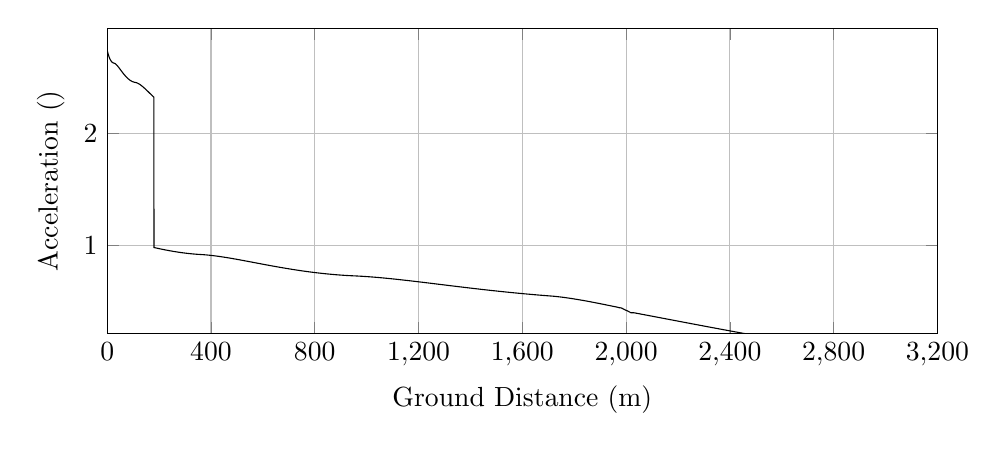
\begin{tikzpicture}

\begin{axis}[
width=\textwidth,
height=0.45\textwidth,
scaled ticks=false, tick label style={/pgf/number format/fixed},
xmin=0.0,
xmax=3200,
xtick={0,400,800,1200,1600,2000,2400,2800,3200},
xlabel={Ground Distance (m)},
xmajorgrids,
ymin=0.21592694018874944,
ymax=2.9383329541999035,
ylabel={Acceleration ($\si{\meter\per\square\second}$)},
ymajorgrids,
]

\addplot [
color=black,
solid
]
table[row sep=crcr]{
1.3729668748937997E-8	2.745933749634024\\
2.6049868369719035E-7	2.7459337463216693\\
2.0491224421327626E-6	2.7459337223163676\\
9.92442121137073E-6	2.74593361664894\\
4.7452367809869807E-5	2.7459331133935008\\
1.740064756114434E-4	2.74593141796994\\
4.0608377013922605E-4	2.7459283128250895\\
7.313431501337001E-4	2.745923966728787\\
0.0011549487327126044	2.7459183141309005\\
0.0016799013484208249	2.745911318665595\\
0.002295089346817705	2.7459031318683342\\
0.003009933382444524	2.745893631784023\\
0.003810608015426248	2.7458830054499908\\
0.004723484476856681	2.745870906509789\\
0.005727138856912631	2.7458576226878897\\
0.006836216967948795	2.7458429637322794\\
0.007997302399386296	2.7458276382144833\\
0.00929136979810952	2.745810580608766\\
0.010685558505459776	2.745792228663979\\
0.012178513621519987	2.745772603889116\\
0.013775244426719659	2.7457516442133327\\
0.015470070176169002	2.7457294279658626\\
0.0172374436815836	2.7457062929339147\\
0.019122918912604377	2.745681646264188\\
0.021104911040230538	2.7456557742244776\\
0.023190717999955576	2.7456285852738693\\
0.025355802981115103	2.7456004025085097\\
0.027620619195902148	2.7455709628304676\\
0.030020274690474198	2.7455398145480876\\
0.032476028269866286	2.7455079832228666\\
0.035054163466719815	2.745474612816359\\
0.037720846868992755	2.7454401452809734\\
0.04049779674511381	2.745404303593875\\
0.043329456594087365	2.745367807581193\\
0.04629652060163805	2.745329620662332\\
0.04934498934704602	2.745290442016606\\
0.052507657924119336	2.7452498537718295\\
0.055769483710642484	2.745208053078813\\
0.05917209570914676	2.7451645112972916\\
0.06264043916012321	2.7451201927906688\\
0.06620063977265622	2.745074766280724\\
0.06987962792775945	2.745027892179869\\
0.0736568184539585	2.744979836976057\\
0.07754284280095361	2.744930469346733\\
0.08151127871105612	2.744880128455919\\
0.08560324933017655	2.744828296550115\\
0.08985265585263943	2.7447745502252845\\
0.09413961367176535	2.7447204093860247\\
0.09857725310864562	2.744664448697618\\
0.10307959255469257	2.7446077566104368\\
0.10766008648593872	2.744550165853771\\
0.11234920964493048	2.744491296646081\\
0.11719267720457946	2.7444305805763873\\
0.12216973960582883	2.7443682839908865\\
0.12724007601918352	2.7443049160916244\\
0.13233299746505212	2.7442413617081813\\
0.13755256756750583	2.744176324555065\\
0.14287728588926696	2.744110077183268\\
0.1482946925752714	2.7440427783081276\\
0.15381585025670613	2.7439742941590106\\
0.15940564092189102	2.7439050633216198\\
0.16526271495916878	2.743832633069937\\
0.17120082448158402	2.743759314593124\\
0.17717889132867753	2.7436856165854584\\
0.18324322596131126	2.7436109697873574\\
0.189427022360885	2.7435349695339406\\
0.1957511558722988	2.743457364727397\\
0.2021484013779125	2.7433789844510024\\
0.20865863707071397	2.743299343476986\\
0.21548666343168166	2.7432159468507686\\
0.22220154781289658	2.743134061837388\\
0.22919671627301902	2.7430488935802986\\
0.23611678795738544	2.742964772871866\\
0.24306300975244904	2.7428804655838492\\
0.2503085190632165	2.7427926639555604\\
0.2576623280401219	2.74270369213178\\
0.26502430524173204	2.7426147629356477\\
0.2724963584449146	2.7425246467856903\\
0.2802001060647876	2.7424318847655185\\
0.2878583985474956	2.7423398174571867\\
0.2958320780323821	2.74224411264151\\
0.3040021452321372	2.7421462114990494\\
0.31208951788619	2.74204945948628\\
0.3202851396023423	2.7419515709453375\\
0.3287233234973125	2.7418509498073105\\
0.3370425959884752	2.7417519080250115\\
0.34575405233845447	2.7416483668644354\\
0.3545073625286812	2.7415445008529415\\
0.36338982075299686	2.74143927707345\\
0.37247557159370037	2.741331824878821\\
0.38151350442869847	2.741225116473271\\
0.3905554764834429	2.7411185361982797\\
0.3999457587520332	2.7410080342749286\\
0.4095398754587949	2.740895325049965\\
0.4189621792151833	2.7407848203234915\\
0.4285208811402964	2.7406729022160494\\
0.43828968955472236	2.7405587157868423\\
0.44807735398784176	2.740444501168418\\
0.45806002753764463	2.740328206966173\\
0.4682994371692033	2.740209125317234\\
0.4787752542918833	2.7400875051939693\\
0.4890770094685154	2.739968111629965\\
0.49985939134273727	2.739843363987376\\
0.5106597490205704	2.739718627718031\\
0.5213580865152188	2.739595283866114\\
0.532247733242454	2.739469951000051\\
0.5431365108549349	2.739344844457758\\
0.554075964429489	2.7392193713226414\\
0.5653450694020941	2.7390903409366887\\
0.5769901159382542	2.738957242270053\\
0.588512657344902	2.738825777773906\\
0.6004070039036553	2.7386903129467894\\
0.6121651247369502	2.738556638601956\\
0.6239717914322569	2.7384226491592862\\
0.6362472885961421	2.7382835883504875\\
0.6486428939173223	2.738143422272314\\
0.6610190736373547	2.7380037294208224\\
0.6737248046101814	2.7378605779440788\\
0.6862826225989949	2.7377193504710986\\
0.6991952542603428	2.7375743971928808\\
0.7122988072688032	2.737427572331951\\
0.7251463703465595	2.7372838790900627\\
0.7381769453061875	2.737138402838057\\
0.7516618647379176	2.7369881315120947\\
0.7654913705221527	2.736834310606014\\
0.7791756406994825	2.7366823919487455\\
0.7930637813125616	2.7365284991417216\\
0.8074774191984457	2.736369088689556\\
0.8215072375247947	2.7362142192435908\\
0.8361010597475598	2.736053431219534\\
0.8503303420601955	2.7358969585996338\\
0.8650627501899835	2.7357352618278403\\
0.8802332960144008	2.7355690814348668\\
0.8951742046771463	2.7354057362911055\\
0.9100334756324657	2.7352435957730297\\
0.9251067343345352	2.735079435666237\\
0.9403923630470314	2.7349132844243806\\
0.9559303815501943	2.7347447191307284\\
0.9712400158034169	2.7345789536451193\\
0.9869533781138684	2.7344091466658877\\
1.0029148609762486	2.734236997780573\\
1.0189962473881624	2.7340638988954913\\
1.035465185745812	2.733886982622522\\
1.0516742337458713	2.7337132054216866\\
1.067815735429615	2.7335404920408557\\
1.0846705971808022	2.7333605047019978\\
1.1012775250051634	2.7331835208984128\\
1.1180798406225687	2.7330048116164747\\
1.1351395900544134	2.7328237286921633\\
1.1526388687279154	2.73263835894707\\
1.1698922447507556	2.732455966615972\\
1.1875468452119025	2.732269712848928\\
1.2058383275300355	2.732077142510799\\
1.2239395537495579	2.731886975352393\\
1.2422020624207541	2.7316955142157697\\
1.2608769472440078	2.7315001426275947\\
1.2794948487006894	2.731305779649479\\
1.2979152553275424	2.7311138807814563\\
1.3166445915281573	2.73091917093961\\
1.3354141707340492	2.730724451882275\\
1.3543210821322504	2.730528719277727\\
1.373689361295591	2.73032863525778\\
1.3932049885015831	2.7301274608942405\\
1.4131781782225183	2.7299220154585475\\
1.4330139682345777	2.7297184263544425\\
1.4528243860883294	2.7295155352372795\\
1.4728783400745615	2.729310592226655\\
1.4934621752870565	2.729100693669997\\
1.5141408097620341	2.7288902940171758\\
1.53430654450827	2.7286855593626536\\
1.5553850389607948	2.728472025774905\\
1.5762653203499473	2.7282609685761434\\
1.5975496774716453	2.728046303569938\\
1.6196077215345106	2.7278243397435746\\
1.6413652536722467	2.727605899295412\\
1.663437310723463	2.7273848044555544\\
1.6860768385032747	2.727158548431424\\
1.7077101022266827	2.726942840558346\\
1.7297306410738114	2.7267237613893585\\
1.7520297891459062	2.7265024111794576\\
1.7743087535215367	2.7262817613558035\\
1.797257424336919	2.7260549980011213\\
1.8200802473615325	2.7258299974170024\\
1.8430350373473994	2.7256042147901303\\
1.8666926279964304	2.7253720605720746\\
1.8902808566018634	2.72514113040999\\
1.9138231309717848	2.7249111877288685\\
1.937187877956735	2.724683506686569\\
1.9611060682733261	2.724450973682445\\
1.9852138445648535	2.7242171481062742\\
2.009780393513653	2.723979437924413\\
2.0346228225622163	2.723739634761041\\
2.0593611988602687	2.7235014085153804\\
2.08477023517836	2.7232573149932806\\
2.110324766702745	2.7230124241566775\\
2.1352655781940433	2.722773991682768\\
2.160528860803022	2.7225330540312687\\
2.1862071157614817	2.722288750937233\\
2.2127756699400534	2.7220366021467237\\
2.2391904543957084	2.721786538650564\\
2.2653528664920257	2.721539475818613\\
2.292150575495974	2.7212870407551826\\
2.3187704640870406	2.721036905412479\\
2.3455495914188482	2.7207858982332622\\
2.372862901366455	2.7205305254301893\\
2.4007145172972395	2.7202707826704753\\
2.428100404243743	2.72001603228333\\
2.4555980306928005	2.7197608861757034\\
2.483374904362833	2.7195038000855876\\
2.511687733451976	2.7192424230947587\\
2.5402569276484597	2.7189793606402857\\
2.568415369317849	2.71872074613543\\
2.596987652715761	2.7184590025560453\\
2.6263861238451423	2.7181903927500546\\
2.655991481965028	2.717920608348247\\
2.6856115886357443	2.7176514041804687\\
2.7154221146045012	2.71738118698586\\
2.7455665152057707	2.7171086712897807\\
2.7752624694325894	2.7168409213882985\\
2.805457625653509	2.71656939071722\\
2.8358231840904597	2.716297056032584\\
2.8663460878589797	2.7160240421896784\\
2.897817297850832	2.7157433103512467\\
2.9287074004595235	2.7154685124985987\\
2.9603588456990284	2.715187708551693\\
2.9922321403815406	2.71490571640717\\
3.0241119471841866	2.71462444530067\\
3.056446055158509	2.7143399570513758\\
3.0889346922121366	2.7140549072190137\\
3.122221620829695	2.713763678408176\\
3.1546991615623394	2.7134803314856493\\
3.187635101478671	2.7131937884197734\\
3.221010117202278	2.7129042459478487\\
3.2543449374576605	2.712615872270808\\
3.288235920596943	2.7123235230382576\\
3.3223704322934555	2.7120299202652527\\
3.3562838593334394	2.7117390566035233\\
3.3906320903803255	2.7114453101597196\\
3.425633159699527	2.711146852210671\\
3.462387235801926	2.7108343880622456\\
3.4973980805087237	2.710537636483595\\
3.5324804241140235	2.710241147744873\\
3.5675385073174235	2.709945728382193\\
3.6040688981843845	2.709638816969628\\
3.6393612181513753	2.7093431890244997\\
3.6770856360342323	2.7090281416612143\\
3.7131729334920323	2.7087276833232927\\
3.749509707933214	2.7084260491268246\\
3.785733977879824	2.7081262444468592\\
3.8225309786916544	2.707822610564083\\
3.860867115351552	2.7075072478509306\\
3.89929745075254	2.7071921001654697\\
3.9373367205567504	2.706881130446619\\
3.9751626485832894	2.7065728578762025\\
4.013671158053867	2.7062599937888168\\
4.0521140617426425	2.7059486353631357\\
4.092377631210638	2.705623567578243\\
4.131586743753305	2.705308027124949\\
4.1715696979561425	2.7049872843873297\\
4.210522654700574	2.7046757949824176\\
4.250196810863292	2.704359538589963\\
4.2917015001093795	2.7040297652367293\\
4.332438976653355	2.7037071511860633\\
4.373124372895289	2.7033859958341147\\
4.414429464889761	2.703061013141131\\
4.455884944705147	2.7027359201134686\\
4.497250153511752	2.7024126010589393\\
4.537976875075978	2.7020953078843215\\
4.581399817640802	2.7017581350427298\\
4.623816269683994	2.701429893974078\\
4.666022338967499	2.7011043708260782\\
4.709098934189642	2.7007732491577343\\
4.752435367147649	2.7004412618628235\\
4.79531009100786	2.700113923220311\\
4.838191999420829	2.6997876304091646\\
4.881381760681686	2.6994601025113845\\
4.9256451804034285	2.6991255802428515\\
4.9704217340957495	2.6987883563581185\\
5.014356093293278	2.6984586198088563\\
5.058826350846283	2.698126010287651\\
5.104458009943745	2.697785910252903\\
5.149663211268795	2.697450177563721\\
5.194981168813841	2.6971147895925576\\
5.241194091283663	2.696773991377621\\
5.287987552078626	2.696430154327218\\
5.334426822383641	2.6960901499960244\\
5.380633359096258	2.6957530602096966\\
5.427524438012913	2.6954122052897027\\
5.476157635197664	2.6950599883398825\\
5.524667120325573	2.6947099813886997\\
5.5732739519824435	2.694360582160768\\
5.6208990292882195	2.6940195060851275\\
5.671502816366864	2.693658464116621\\
5.719824083529298	2.6933150154219874\\
5.767871110439133	2.6929747772519512\\
5.8169321963676754	2.6926286501345027\\
5.866076914057565	2.6922832358810025\\
5.917200682776528	2.691925289335387\\
5.96684810088939	2.6915790178532983\\
6.016885842403935	2.691231352228524\\
6.068639931677712	2.6908731577503717\\
6.119867755785197	2.6905199976544543\\
6.171030794930029	2.6901686602208663\\
6.222884713227881	2.6898139753337107\\
6.2735946138732235	2.6894684695538738\\
6.325883502103322	2.6891136013011465\\
6.379615386553551	2.6887504096481347\\
6.432194972482147	2.688396442468087\\
6.484528316464761	2.6880455368872473\\
6.536619297696934	2.68769764118571\\
6.589662958081361	2.687344796419861\\
6.644121795496577	2.6869840153423956\\
6.697445536614451	2.68663219810922\\
6.7518063163896365	2.686275003043974\\
6.8068829439682315	2.685914605406988\\
6.863205650636274	2.685547609679398\\
6.9185329265047315	2.685188625021353\\
6.974634519184049	2.684826152672259\\
7.031139830722298	2.6844626288388405\\
7.0870923879294985	2.6841041940757817\\
7.144766952910487	2.6837363176346836\\
7.2026451873548805	2.683368757231797\\
7.261191729679483	2.682998591553873\\
7.320502240843062	2.682625268876813\\
7.378210233177999	2.6822636424501294\\
7.437738452534925	2.6818922655745236\\
7.49714639104333	2.681523308417665\\
7.556502460410064	2.6811563316145213\\
7.617032771987237	2.680783794499826\\
7.676883327249088	2.6804171211405423\\
7.735740247984193	2.6800581575988813\\
7.796086087039788	2.679691776501249\\
7.856787102853412	2.6793249307229674\\
7.91721236259451	2.678961429481797\\
7.979013602666894	2.6785913752038963\\
8.039824025454376	2.6782289487607027\\
8.102419182184594	2.6778576340357727\\
8.16459313580776	2.6774905665511346\\
8.226347093952135	2.677127696565849\\
8.290527749984296	2.676752373844961\\
8.353592793320257	2.6763853613705777\\
8.417564177281012	2.67601487568339\\
8.482044607535009	2.675643270078857\\
8.547336806956285	2.6752688485572547\\
8.613293246319614	2.6748925126021685\\
8.6778048537894	2.6745262550450724\\
8.74454839911753	2.674149227258674\\
8.810708373588199	2.673777396453808\\
8.876548424968423	2.673409234250302\\
8.942828456712885	2.6730404887927257\\
9.010858044488913	2.6726639601609223\\
9.079453414959548	2.6722862922314583\\
9.148767802603732	2.6719066890561036\\
9.21609997183467	2.6715398811000908\\
9.285579683381485	2.67116336940079\\
9.355451712480097	2.670786767326205\\
9.423585014597279	2.670421494476032\\
9.493435356703696	2.6700490148237135\\
9.562655940911181	2.6696818813962357\\
9.63183713653898	2.669316926216502\\
9.703018708836247	2.6689434650398702\\
9.773178624863132	2.6685773872877823\\
9.844376937811855	2.6682079365263496\\
9.914998792594716	2.6678435040567887\\
9.98720270419701	2.6674729864037268\\
10.059478150570087	2.6671041981501142\\
10.132362020358627	2.6667344209387407\\
10.205876892438312	2.6663635857706476\\
10.279422251887688	2.6659947421935097\\
10.353305644514993	2.6656263553136483\\
10.42811398108589	2.6652555454284528\\
10.50332954727428	2.664884928557493\\
10.578207710262959	2.6645181680900603\\
10.65503529959097	2.6641441252244062\\
10.730232142651953	2.6637802356245537\\
10.805871937852555	2.6634164032193377\\
10.88265320376452	2.6630493287809767\\
10.958577899345514	2.6626885682826185\\
11.034861147941964	2.662328317504069\\
11.112742623646977	2.6619627989513033\\
11.190543636431041	2.661599949051814\\
11.267787598939979	2.6612419536263943\\
11.3462805052093	2.6608804641262784\\
11.423875697147409	2.6605253733666894\\
11.502735831556972	2.66016679186927\\
11.581465323066688	2.6598111062891867\\
11.661639233340708	2.6594512496614984\\
11.741743247575428	2.659094070532034\\
11.821864700430528	2.6587391681041073\\
11.901816327719768	2.6583873562373483\\
11.98361062800689	2.65802984404648\\
12.065425957085825	2.657674667049518\\
12.1478520915771	2.657319283720091\\
12.230956215923495	2.6569634524950505\\
12.313306905825911	2.6566132897052395\\
12.396632357805931	2.656261447402212\\
12.479578787946746	2.655913659143116\\
12.564327762802186	2.6555608318228234\\
12.648175874147956	2.655214251081233\\
12.736145481689512	2.6548532930755826\\
12.821080154398764	2.6545073614738826\\
12.908009536077355	2.6541559136608868\\
12.994986774303499	2.6538069029568296\\
13.081752199798046	2.6534613540348904\\
13.17035388279784	2.6531111740371047\\
13.257836697901475	2.652768065088189\\
13.34511613365563	2.652428366974772\\
13.433461823066896	2.6520871672573874\\
13.524108483575919	2.6517398400805456\\
13.611203924103116	2.6514087427638877\\
13.702229394080796	2.6510654420726993\\
13.792427706753081	2.650728010041674\\
13.882429934062493	2.6503940290968764\\
13.975435778888343	2.650051743756091\\
14.065832730112316	2.6497218173613817\\
14.157894546480026	2.649388598244756\\
14.250668806951023	2.649055631782466\\
14.343291987615704	2.6487260325270725\\
14.43744444968501	2.64839387373258\\
14.532636396723657	2.6480609912501123\\
14.625507232812737	2.6477390675021404\\
14.721503924398366	2.6474092478024884\\
14.818738382089133	2.6470782104461428\\
14.913572076739943	2.6467582780736505\\
15.009701633366973	2.6464369177531655\\
15.10815424447124	2.6461108524555685\\
15.206130868840724	2.6457894275225193\\
15.304035939715973	2.6454712794394446\\
15.403499839366233	2.645151168619309\\
15.503209871950865	2.6448333932172794\\
15.601718454553605	2.6445225108434887\\
15.700655560608023	2.6442133305209685\\
15.801250929860519	2.6439020954003567\\
15.899917805652187	2.643599879299895\\
16.001574124100856	2.6432916569963822\\
16.102638779863817	2.6429883870635598\\
16.204479333764816	2.6426859631921458\\
16.30489644092564	2.642390875444015\\
16.40578186591999	2.6420975095348966\\
16.509201471948074	2.641799986524223\\
16.614557195984908	2.6415002256988815\\
16.717657554831042	2.641210126302675\\
16.823039336622365	2.640916912552081\\
16.928576062495388	2.6406266046044653\\
17.03469945574068	2.640338038396731\\
17.140697318244236	2.640053160739731\\
17.246066414787876	2.639773277049187\\
17.35183930840021	2.639495622702711\\
17.458399953804133	2.639219234411631\\
17.565707112453843	2.6389442799060117\\
17.673103795073075	2.638672470550473\\
17.781888038667653	2.638400579402105\\
17.89115167195854	2.6381309531423165\\
18.00105710767307	2.63786323255278\\
18.110142905530395	2.6376009574466197\\
18.219697237410173	2.637341002414172\\
18.32752951944549	2.6370884953076636\\
18.43743745973078	2.6368345484445737\\
18.54904630654982	2.63658019384358\\
18.659302591714813	2.6363323952736817\\
18.770734536087716	2.636085450694776\\
18.883577445650936	2.635838949357387\\
18.996263390583444	2.635596364184675\\
19.108816920034535	2.635357616908477\\
19.22287647779894	2.6351192855805\\
19.33763586704334	2.6348831480062795\\
19.456324114791514	2.6346427711361047\\
19.57349394116079	2.634409291852097\\
19.690148252848566	2.634180600096859\\
19.80521137071168	2.633958691418372\\
19.92379170801214	2.633733794227746\\
20.04216631061405	2.6335131166802155\\
20.15848954929409	2.6332999786096893\\
20.278242138037896	2.6330843918964613\\
20.396206084226087	2.6328758170334643\\
20.516315546862906	2.632667302876359\\
20.637173924977112	2.632461401533406\\
20.75450010628387	2.6322652607421713\\
20.874378237858778	2.632068650375719\\
20.996035953832852	2.6318730325170687\\
21.11812959618858	2.6316806625120934\\
21.240471115580952	2.631491857446668\\
21.361479376438375	2.6313089928781865\\
21.485224699488654	2.631125973433857\\
21.607870280890317	2.6309485406063304\\
21.73242999733349	2.630772361329301\\
21.85704493170313	2.6306001480967662\\
21.98122016226351	2.6304325538620574\\
22.10826921766411	2.6302652125995127\\
22.235261614051304	2.6301021093246337\\
22.361664688868032	2.629943883831288\\
22.48780138980522	2.6297900776934346\\
22.614107216476143	2.6296401428980527\\
22.74409311379692	2.6294900871360998\\
22.873024137794893	2.6293454925824022\\
23.003512644166257	2.6292034414201826\\
23.132891545907036	2.629066846405708\\
23.26270690888247	2.628934029456868\\
23.39264146728729	2.6288053298831127\\
23.52277721573431	2.6286806696961964\\
23.654883767164463	2.6285584477188975\\
23.78569183677709	2.6284417091087624\\
23.917003007077597	2.628328794588147\\
24.047013652206026	2.628221204195908\\
24.178458227988493	2.6281166694027984\\
24.314609552493202	2.6280128759318746\\
24.447533097503474	2.627915932898171\\
24.579128452041708	2.627824218719879\\
24.71011994849615	2.627737123338611\\
24.843278471916108	2.627652868038229\\
24.975761222328053	2.6275733117861915\\
25.1115496753864	2.6274961796102385\\
25.247101122854083	2.627423621584068\\
25.384906965000688	2.627354391118195\\
25.522261036073317	2.6272899242628656\\
25.66123001648475	2.627229296090176\\
25.79865327455613	2.627173876444852\\
25.826335196219034	2.6271632574604533\\
25.839610403727477	2.62715822969495\\
25.841006316401874	2.627157703174394\\
25.84227013303559	2.6271572259940434\\
25.84770509053729	2.6271551682557828\\
25.86419328224909	2.627148869514051\\
25.90571916957557	2.627132632727095\\
25.999268866927544	2.62709410603191\\
26.123295978662824	2.627038901212371\\
26.250212562581652	2.6269775933396176\\
26.376891976518465	2.626911599588503\\
26.50638698165423	2.6268392423555404\\
26.634042370994827	2.6267631265942892\\
26.763333806613538	2.626681250837172\\
26.893207366259766	2.62659421847878\\
27.022905486492228	2.6265025738361114\\
27.153956322362554	2.626405232066988\\
27.287774297957696	2.626300978647955\\
27.42030033806219	2.6261929566003683\\
27.555504894698295	2.626077916748084\\
27.691130018821354	2.6259576762016144\\
27.82633313037239	2.6258330443348266\\
27.959508564917073	2.625705689812035\\
28.096515548835796	2.6255699768647354\\
28.232789703382153	2.6254303281033025\\
28.368684388406535	2.625286498680893\\
28.506541650227618	2.6251359904785243\\
28.64533374691623	2.624979841336361\\
28.78297783415192	2.624820465669056\\
28.92277775692753	2.6246540493487274\\
29.06227187463503	2.624483493060775\\
29.20212864139956	2.6243080372215513\\
29.34335827861657	2.624126392094661\\
29.483225747293005	2.623942134485322\\
29.625960812476485	2.623749682168036\\
29.76706561118049	2.6235551018597727\\
29.909402910999468	2.6233545237810842\\
30.051751399473822	2.623149671618658\\
30.196612335666572	2.6229368923312792\\
30.342192969749448	2.6227187353115538\\
30.48583400527584	2.6224992991267593\\
30.632658550781265	2.622270763203243\\
30.77846394498075	2.6220396350772806\\
30.92408133049836	2.6218047080288107\\
31.071091331299215	2.6215634400823893\\
31.218274793935116	2.6213178254024356\\
31.366705758252415	2.6210660719563164\\
31.515339333797037	2.6208099515408767\\
31.66356819769615	2.620550577189582\\
31.814689402684216	2.6202821391202162\\
31.96649953392354	2.6200084685109024\\
32.115424616034375	2.6197361526902787\\
32.266253234088566	2.619456531320976\\
32.41813832080348	2.6191711196609058\\
32.569791431087395	2.6188823653016966\\
32.722234201183724	2.618588359660447\\
32.876984607664	2.6182861188418736\\
33.031873994672836	2.6179798472058744\\
33.18502245018544	2.61767337730517\\
33.34135780547538	2.6173568541876238\\
33.49759920343199	2.6170368690402794\\
33.65385117142162	2.6167132684054444\\
33.8113313806527	2.6163835453824538\\
33.96985264489639	2.6160480723691215\\
34.126473036379195	2.6157131607910555\\
34.2857505660089	2.6153690959358693\\
34.4449212019973	2.6150218218705428\\
34.60566879064274	2.6146676745052684\\
34.76644486933921	2.614310071010496\\
34.92612701881755	2.613951597544056\\
35.08630421658309	2.6135887608266746\\
35.24825698849928	2.613218646437778\\
35.412303951281956	2.6128404656979436\\
35.57355277914179	2.612465573208352\\
35.73545353069308	2.612086065190393\\
35.89925038949356	2.6116990063305368\\
36.065161289279985	2.611303822719635\\
36.23047312008262	2.6109069894047563\\
36.39472205714358	2.6105097203642957\\
36.56135389445764	2.6101036997752756\\
36.72774532558607	2.609695316287241\\
36.89384825683493	2.6092847556652456\\
37.05904296416534	2.608873633171015\\
37.22702676294645	2.6084527521107095\\
37.39437475321985	2.6080306918927274\\
37.5621109943643	2.607604928234461\\
37.73270471709142	2.607169167240153\\
37.903359519601935	2.6067305347705387\\
38.071486842086316	2.6062957943756917\\
38.23815243703595	2.6058623319798837\\
38.40817787072022	2.6054176148453294\\
38.57751392140098	2.604972224462812\\
38.750215798728505	2.604515486819169\\
38.92001182640311	2.604064028086343\\
39.09310637700479	2.6036013939253158\\
39.26472366117933	2.603140360230884\\
39.436554723976656	2.6026764590104268\\
39.608961777617054	2.602208745072529\\
39.782828308010565	2.6017348303452126\\
39.956194359016465	2.6012600869258415\\
40.132391837044906	2.6007753954833523\\
40.30868053167249	2.6002882883371417\\
40.48611580488176	2.599795875967091\\
40.66383502946924	2.599300575623608\\
40.83999042132467	2.5988076076289266\\
41.018202681018664	2.598306879012876\\
41.19780999006247	2.59780023921822\\
41.37730467548502	2.5972919679986406\\
41.557010452813884	2.5967811949022925\\
41.73612816026986	2.5962702442991796\\
41.91555194917056	2.5957566162813004\\
42.09743589423803	2.5952341495078093\\
42.27807550146298	2.5947135135520316\\
42.45995188234755	2.594187603754664\\
42.6401410478328	2.593664926422731\\
42.822293873795985	2.5931349327029034\\
43.00585672428667	2.5925992336587598\\
43.189965171449515	2.592060371841985\\
43.372020236704074	2.5915260176090396\\
43.555636897252796	2.5909856106444664\\
43.74012033961118	2.5904412105939336\\
43.92429822300048	2.5898963139394615\\
44.106869824379004	2.5893548329369107\\
44.29411840239129	2.588798141810776\\
44.47920670866131	2.5882465834656143\\
44.665034305215386	2.5876915745572395\\
44.85242224248053	2.5871306821366113\\
45.03948098831597	2.5865695920897522\\
45.22811764277584	2.586002614453135\\
45.41548629589063	2.5854383417605273\\
45.60322541388645	2.58487188864763\\
45.793007222766036	2.584298230300096\\
45.983742663331824	2.583720675421648\\
46.172643153142886	2.58314771556424\\
46.36421599110457	2.582565713945945\\
46.553512793459404	2.5819897407332553\\
46.745018895697555	2.5814061887802406\\
46.93606459490553	2.580823220829023\\
47.126948089509526	2.580239969889381\\
47.31881294044018	2.579652975509168\\
47.5110690178297	2.5790640736859434\\
47.705448624448266	2.5784679831468953\\
47.90005519882567	2.577870546429364\\
48.09288923506665	2.577277947636331\\
48.28732881729917	2.576679844114947\\
48.484002572746206	2.5760743233998253\\
48.68089030454945	2.575467633349363\\
48.87532723390382	2.57486803095897\\
49.07073736177763	2.5742649991859343\\
49.2672083392297	2.5736582972862303\\
49.46586249263092	2.5730444865995894\\
49.661880987188695	2.5724384938105347\\
49.85966148345089	2.5718267615262587\\
50.05808618672894	2.571212777407524\\
50.25785665917266	2.570594402569249\\
50.45743808511885	2.569976421527972\\
50.65573800086891	2.5693622538365988\\
50.85948768734909	2.5687310825359084\\
51.061243703011925	2.5681059980424292\\
51.26368286286315	2.567478743109982\\
51.46416466063809	2.566857533975103\\
51.66475943174029	2.5662359893110347\\
51.86588207153103	2.56561285677663\\
52.07444928962187	2.564966744465173\\
52.2824430085781	2.5643225310284814\\
52.48676525705545	2.5636898422625745\\
52.69531994892206	2.5630442386830037\\
52.90027076850366	2.562410012697458\\
53.108186167814935	2.5617668705752035\\
53.31165724918766	2.561137759462768\\
53.520024946679996	2.560493831718171\\
53.72688450142306	2.559854920280424\\
53.93707391647578	2.5592061198138465\\
54.14518573319289	2.5585641573342945\\
54.35125853722778	2.5579289322446064\\
54.56213447502874	2.5572793940255876\\
54.77598621923464	2.5566212311207\\
54.987629956235494	2.5559704324655836\\
55.19778857845695	2.5553247914147734\\
55.41030974885841	2.55467252202679\\
55.62390503323701	2.554017625167454\\
55.83671574169797	2.553365831759879\\
56.047071254351536	2.5527222723040826\\
56.26137331252919	2.5520673989185383\\
56.47512769358855	2.5514149930840677\\
56.69105800830218	2.55075678108659\\
56.90937011004422	2.5500921924420785\\
57.12736617899088	2.549429482767894\\
57.346833156368504	2.5487632574065238\\
57.56476609337061	2.5481026676419045\\
57.78230894703917	2.547444262133678\\
57.99943865551505	2.5467881336539273\\
58.21827465292657	2.5461279153126446\\
58.436085045729726	2.545471882108224\\
58.6577546799423	2.5448053710641405\\
58.87982836766625	2.544138832936956\\
59.10336118170943	2.5434691447546607\\
59.324182403931715	2.542808819305696\\
59.545440661451366	2.5421484495030766\\
59.768227251413464	2.5414848224466517\\
59.99077485409802	2.540823240966116\\
60.21631063559073	2.54015416369662\\
60.44006004384342	2.539491792913134\\
60.66502706168687	2.5388272572727564\\
60.89133011288284	2.5381602583073883\\
61.11585558357916	2.5374999948556693\\
61.3432655409558	2.5368327945800493\\
61.57186440401435	2.5361637002878803\\
61.79868765088207	2.535501408748763\\
62.025670725987	2.5348402770909786\\
62.254132946411545	2.5341765056009926\\
62.48290793247415	2.5335135279774255\\
62.713817944074236	2.5328461162466924\\
62.94484116346062	2.5321801651283318\\
63.17805109236767	2.5315097497788024\\
63.41124119062552	2.530841264404774\\
63.64505576847972	2.5301728944345925\\
63.87735201907903	2.5295107788661895\\
64.11169045660182	2.5288448001638137\\
64.34725756208485	2.52817733598523\\
64.58324360279937	2.527510726208688\\
64.81881329818131	2.5268473544899654\\
65.05563560606473	2.5261825559991893\\
65.29467812810154	2.5255136850947695\\
65.53178653633495	2.524852393698131\\
65.77046761369158	2.5241889200770515\\
66.01019347650049	2.523524791474693\\
66.25262920761091	2.52285547188822\\
66.49342175078831	2.522193018006006\\
66.73393309567928	2.5215336779391944\\
66.97718905970893	2.52086921586132\\
67.21919788222482	2.5202105803525665\\
67.46413738735515	2.519546449583455\\
67.70584739194695	2.518893544044623\\
67.95375887035246	2.5182264574902717\\
68.19817148521656	2.5175713561374016\\
68.44413350233111	2.5169147004876002\\
68.68984243621705	2.516261345089669\\
68.93951041285982	2.515600171501796\\
69.19023531750676	2.514938969433662\\
69.43956667494601	2.514284217583624\\
69.68998597860525	2.513629416130965\\
69.94098943220166	2.512975932155717\\
70.1928405184459	2.5123231255440013\\
70.44659484061637	2.511668329081634\\
70.69926103579675	2.5110192971929557\\
70.95414956377036	2.5103675673854084\\
71.21136313866151	2.5097129793716446\\
71.46778788208749	2.509063506597747\\
71.7247351381395	2.5084158438377147\\
71.98234155897126	2.507769689085089\\
72.24107377350035	2.5071239256193767\\
72.4986091150376	2.5064843695454924\\
72.75949164810788	2.505839797213234\\
73.02014691132015	2.505199119753618\\
73.28114866838587	2.504560949336046\\
73.54342372888959	2.503923071226774\\
73.80584407854005	2.5032882764078206\\
74.07231166191039	2.5026472290607487\\
74.3389341302921	2.5020093971959803\\
74.60521354141642	2.501375988177486\\
74.87280568706873	2.5007431028336446\\
75.1403821105715	2.5001139292433843\\
75.41145333671997	2.4994803046180856\\
75.68265298797411	2.4988501932497016\\
75.95075857762194	2.498231039158717\\
76.2241428819712	2.4976035721719434\\
76.4990100438061	2.496976668570306\\
76.77213586328236	2.4963576955699853\\
77.04724851790667	2.49573822862106\\
77.32330034006353	2.4951207098630084\\
77.59850473375684	2.4945091566067346\\
77.87773830129439	2.4938928219842715\\
78.1565255546137	2.4932816837060106\\
78.43842651648492	2.492668017346257\\
78.720833678605	2.4920576010425153\\
79.00101298089581	2.4914563231480757\\
79.28359351218376	2.4908542717934887\\
79.57011733099088	2.490248328576058\\
79.85418914588558	2.4896520718283295\\
80.13919871477489	2.4890583687052414\\
80.42568449319114	2.4884661731421938\\
80.71472498530085	2.487873370981382\\
81.006853148924	2.487279025102887\\
81.2951972638476	2.4866971170884167\\
81.58524575795963	2.486116537145639\\
81.87461709596036	2.4855420949920353\\
82.1711642895769	2.484958381559892\\
82.46716486408064	2.484380782761332\\
82.76422974563803	2.483806186216814\\
83.05801377197795	2.483242957146957\\
83.35853301954708	2.482671999870737\\
83.65664966506407	2.4821108049392793\\
83.95487262936624	2.481554606519677\\
84.25322789115987	2.4810033792257986\\
84.55664509033022	2.4804481694309706\\
84.8599544590121	2.4798985860092557\\
85.16499148084048	2.4793513638033664\\
85.47187188044902	2.478806409028219\\
85.77908321853027	2.4782664837735044\\
86.08675489504844	2.4777313991684684\\
86.39784539041122	2.4771961342162765\\
86.71051296037359	2.4766640142286205\\
87.02583358957506	2.4761333445033173\\
87.34037846285594	2.4756099658506825\\
87.65395388450591	2.4750941674588303\\
87.96687312379424	2.4745854039580317\\
88.28527441497255	2.474073850456792\\
88.6103524516937	2.4735579588692937\\
88.92871226770333	2.4730590021066936\\
89.25003295857354	2.472561715850354\\
89.57522243846881	2.472064913921284\\
89.90247582737899	2.4715715482953424\\
90.22602529632545	2.471090281458441\\
90.5494223037065	2.4706157304863785\\
90.87816525326718	2.470140000358535\\
91.20455861430293	2.4696743344984124\\
91.53817773235312	2.4692052383281\\
91.87076195087604	2.46874453523425\\
92.20124984301029	2.468293613714687\\
92.53140503523474	2.4678500072923946\\
92.86389705561814	2.467410207209607\\
93.19815266874983	2.46697511608851\\
93.53304529783748	2.4665462917878456\\
93.86737084100128	2.4661252936021194\\
94.20337949361911	2.4657093387407842\\
94.54065981474497	2.4652990463300517\\
94.87396787418089	2.4649007234996034\\
95.21684847579547	2.4644983797555815\\
95.55392648231228	2.4641101935898275\\
95.89232371872416	2.463727831543161\\
96.23051075783204	2.463353072193108\\
96.57164052232307	2.4629825255521096\\
96.90762523479154	2.4626249186321765\\
97.24755293575913	2.462270552927021\\
97.58790661409188	2.4619232523826478\\
97.92576087813703	2.461585947168559\\
98.26661027452474	2.4612531815923795\\
98.6051908024865	2.4609301321117414\\
98.94563962387357	2.4606128512157275\\
99.28665364663627	2.4603026475156407\\
99.63350087797645	2.4599949576702347\\
99.97685593767679	2.4596981466115277\\
100.31593955776762	2.4594126383431973\\
100.65572384630482	2.4591341387793317\\
100.99616871909686	2.4588627388350837\\
101.3402339503516	2.458596236175948\\
101.67973054404297	2.458340953841132\\
102.01657591573795	2.4580952179760907\\
102.35656456518868	2.457854829697289\\
102.6941824316649	2.457623725275984\\
103.03547296258705	2.457397823628013\\
103.37623032340073	2.457180026797986\\
103.71852978299776	2.456969054425172\\
104.05851119314701	2.4567672705298635\\
104.3949509202441	2.4565752126830196\\
104.7329053851843	2.456389936423986\\
105.07104272194636	2.456212240406991\\
105.40742307340048	2.456043101164078\\
105.74423560014887	2.4558813834138933\\
106.07955743077031	2.455727984822288\\
106.41623710643992	2.4555816081016255\\
106.75618472497374	2.455441591416804\\
107.0942647435474	2.4553101084432747\\
107.43151869252583	2.4551866717490167\\
107.44650965670576	2.4551813642403237\\
107.45815118347005	2.4551772531208176\\
107.46233674961977	2.4551757772689795\\
107.46535588765028	2.4551747132015054\\
107.46808502617694	2.4551737507643727\\
107.4836206108138	2.455168259670489\\
107.53176708907421	2.4551511079163477\\
107.68672244793561	2.455094531599669\\
107.97570433527497	2.4549834451948627\\
108.27744765146667	2.4548597682328195\\
108.5816623935838	2.4547272061477434\\
108.88557241638279	2.4545869610121596\\
109.19209959959528	2.45443767243568\\
109.50241879336687	2.4542786003150896\\
109.81066605766154	2.4541127633367736\\
110.12101503747155	2.453937994054648\\
110.43285681965125	2.4537545790192175\\
110.74725799716322	2.453561818956234\\
111.06462449033057	2.4533593397004765\\
111.38211128519615	2.453148923592198\\
111.70119562731901	2.4529296108117045\\
112.02298633508096	2.452700564309909\\
112.34320819983824	2.452464869014065\\
112.66812620709393	2.452217884637398\\
112.99302416686388	2.451963112159949\\
113.31966045518399	2.4516991968576756\\
113.64998129974768	2.451424459279832\\
113.97857627498675	2.451143416865058\\
114.31304608469316	2.450849510906499\\
114.64448318111735	2.4505505571921855\\
114.98093514978115	2.4502393175308965\\
115.31969924418831	2.4499181287839766\\
115.65790718621022	2.449589741128423\\
116.00063352526521	2.4492491841404753\\
116.34235083463872	2.448901923487149\\
116.68621873349733	2.448544803075687\\
117.03331062078092	2.4481766222286128\\
117.37910048629482	2.4478022122028253\\
117.72869476105836	2.447416056567934\\
118.08005947084649	2.447020315368726\\
118.43363644355449	2.44661445841039\\
118.79186464668504	2.446195562722882\\
119.14769212941735	2.4457719010897243\\
119.5036618261702	2.4453406161077478\\
119.86270697471275	2.444898151431988\\
120.22616362054572	2.4444427272159954\\
120.58991121293201	2.4439794620158324\\
120.95538130513773	2.443506572675182\\
121.3195355377388	2.4430280793612997\\
121.68590041554987	2.4425394226513815\\
122.05305648207542	2.442042507730611\\
122.42257239354896	2.4415352206266228\\
122.79503144936103	2.4410167087569397\\
123.16629137010841	2.4404927909789507\\
123.53950748252527	2.439959095724661\\
123.91239367862553	2.4394189483888704\\
124.29026003316017	2.4388646308631676\\
124.66301933937496	2.438311045841078\\
125.03890311735066	2.4377461242287524\\
125.41380975776434	2.4371760734767376\\
125.7896808967325	2.4365980418067945\\
126.16837244152023	2.4360091772577572\\
126.54595968852882	2.4354156387065453\\
126.92471834906405	2.434813947054397\\
127.30294276405039	2.4342068948637348\\
127.68255852126984	2.433591469128208\\
128.06243727540487	2.4329695571547303\\
128.44360431740483	2.432339541404442\\
128.82265748788262	2.4317071612453454\\
129.1989690567886	2.4310736703116387\\
129.57765386613931	2.4304305602421765\\
129.95508099647026	2.429784065084977\\
130.33359114840187	2.4291302715149827\\
130.71373745886524	2.4284682576146626\\
131.09453904397424	2.4277997749107643\\
131.47657586018488	2.4271238577704235\\
131.85678563989967	2.426446027201812\\
132.23856625352113	2.42576032125654\\
132.61595336405918	2.4250775964184523\\
132.99976263915818	2.4243783357290276\\
133.38083522978053	2.423679242984316\\
133.76098428781995	2.4229771481541835\\
134.1363519425165	2.4222793654313444\\
134.51557915495124	2.421569932295995\\
134.8968696170101	2.4208521881638854\\
135.27419431482667	2.420137597883574\\
135.65215477207505	2.4194175854598914\\
136.03329358991255	2.4186873250908105\\
136.41192880753374	2.4179577730609862\\
136.7898079310749	2.417225694571063\\
137.17001317148595	2.4164851729427035\\
137.54844558779996	2.415744261492118\\
137.92617219433072	2.4150009862160164\\
138.30476964659732	2.4142523189260237\\
138.68390038934075	2.413498983015482\\
139.0631653430654	2.4127418378009757\\
139.4406106933401	2.41198488197385\\
139.81914660512416	2.4112223633220573\\
140.19767098864742	2.410456560906317\\
140.5730919292459	2.4096938425620706\\
140.95061983253072	2.4089237067743268\\
141.32838502869612	2.4081500093041033\\
141.70636515873298	2.4073728610224387\\
142.0839785067887	2.406593529688587\\
142.46357402350594	2.4058072184921997\\
142.84082211769783	2.40502296889394\\
143.21906727224075	2.4042339114596416\\
143.59963619096823	2.403437310882776\\
143.97984478872678	2.4026388326905357\\
144.35941603837455	2.4018391364099507\\
144.7355521893594	2.4010442230400466\\
145.11296635073694	2.4002442180265584\\
145.49073213867456	2.399441133914113\\
145.87033631970945	2.3986318541955978\\
146.24486520181193	2.397831210000894\\
146.6238757206513	2.3970188391759493\\
147.00096360401335	2.396208508945593\\
147.37874202190085	2.3953946757121454\\
147.756852900845	2.39457816388311\\
148.13572640408995	2.393758097000817\\
148.5136798644104	2.392938178662493\\
148.89083780486442	2.392118210713834\\
149.2712459042852	2.391289439886328\\
149.65303236723025	2.390455972301191\\
150.0329584616291	2.389624940771009\\
150.41363382646614	2.388790702960881\\
150.79322940570728	2.3879573271300165\\
151.17272478467066	2.3871227269328097\\
151.55400296227282	2.3862828087520374\\
151.93482601265913	2.385442551958211\\
152.31881414221942	2.3845940116132027\\
152.70208150063132	2.3837458190581575\\
153.08320649997165	2.382901190023449\\
153.4666285558243	2.382050340959543\\
153.84825937276264	2.381202396702336\\
154.23093781718723	2.380351107148919\\
154.61485031834388	2.379496102763693\\
155.00001234931443	2.3786373939872023\\
155.38285725409855	2.3777829898524283\\
155.7679513537659	2.3769227531344317\\
156.1509667875323	2.3760664034774726\\
156.53491934392343	2.3752072536116557\\
156.91995289130983	2.37434502792717\\
157.30625057946366	2.373479362158138\\
157.69121706207227	2.3726161237217385\\
158.07789765133754	2.371748534188164\\
158.46521012398495	2.3708790680405922\\
158.85138765236047	2.370011742814021\\
159.23964669847322	2.3691393833615075\\
159.62715395386465	2.368268403666744\\
160.01960115328984	2.367386056204964\\
160.4079207075476	2.366512776596168\\
160.79602490671402	2.36563981902208\\
161.18437278725975	2.364766199221803\\
161.57644284003254	2.363884138972799\\
161.96812230097612	2.363002938647095\\
162.35808768568592	2.362125623778489\\
162.75087300343483	2.3612420420191382\\
163.14546270495134	2.3603545272165904\\
163.53745675514648	2.3594730228399685\\
163.92955389373896	2.3585915050473067\\
164.32395276810763	2.357705079439211\\
164.71713266653478	2.3568217061873185\\
165.1102153740033	2.35593890902884\\
165.5035884424101	2.355055863096327\\
165.89816400198282	2.3541705682312966\\
166.29148626774366	2.3532885788431104\\
166.68861804276264	2.3523985917182593\\
167.082852347146	2.351515683455717\\
167.48006204110857	2.3506267458495653\\
167.8798182678497	2.349732796398407\\
168.27774435731556	2.3488436682392644\\
168.67741362640317	2.3479514207768712\\
169.07475368467374	2.3470651868695898\\
169.4759958044982	2.3461711163376826\\
169.87832784425882	2.3452755349517966\\
170.2792240364854	2.344384106753197\\
170.68126852540456	2.3434911272918937\\
171.08617821288442	2.3425928410644596\\
171.48766933901368	2.341703228415432\\
171.892744970828	2.340806814987485\\
172.29711201372032	2.339913155185136\\
172.70264003426053	2.339018160916506\\
173.1105289448074	2.3381192418897934\\
173.5163733808056	2.337226149563117\\
173.92577914808027	2.336326596791209\\
174.33607303977334	2.335426521117654\\
174.74614233406845	2.3345284082190787\\
175.15731444736514	2.3336293965914052\\
175.56901623635082	2.3327307892227083\\
175.97955109701695	2.3318363258755\\
176.39275298155184	2.330937702273025\\
176.80397138375372	2.3300450760546294\\
177.21946344336607	2.329144919042588\\
177.6332252263685	2.3282502942964154\\
178.05102033212842	2.3273487947563245\\
178.46725124888752	2.3264525543676644\\
178.88389799206544	2.325557341115923\\
179.29839533747668	2.324668693141324\\
179.71608569665375	2.3237752025766305\\
180.1342696339205	2.32288270874726\\
180.26454521656194	0.9819097825897585\\
180.5538779958007	0.9815536538867426\\
180.97677279803082	0.9813338843741317\\
181.73177043104909	0.9809420613829676\\
182.61825861954026	0.9804828804582393\\
183.4994266290775	0.9800274114937022\\
184.38832398643513	0.9795689259516667\\
185.2752206450968	0.9791124645948044\\
186.16090254585617	0.9786576300079914\\
187.05782443666988	0.9781980558527161\\
187.95004436743	0.9777419344260561\\
188.84343565256296	0.9772862693797477\\
189.73203483232732	0.9768341080623215\\
190.63087969896367	0.9763778205536682\\
191.53167348748025	0.975921653048007\\
192.42914206966827	0.975468285978192\\
193.32936064878362	0.9750146613483333\\
194.23353734669462	0.974560195085505\\
195.14873951553636	0.9741013759586223\\
196.05846844349168	0.973646498220359\\
196.9665797060448	0.9731936319952481\\
197.88137813217617	0.9727386577834067\\
198.80153314772656	0.9722822736673473\\
199.72262566550114	0.9718266963438293\\
200.6418018332526	0.9713733471887152\\
201.57021605131746	0.9709167520076665\\
202.49227039761405	0.9704645997371386\\
203.4093310979173	0.9700162077043244\\
204.33741716634955	0.9695637680397735\\
205.26228808295895	0.9691142513984239\\
206.1977933698634	0.968660954442008\\
207.13719708861407	0.9682071851823584\\
208.07111616454222	0.9677574839439917\\
209.00693662932974	0.9673082974336158\\
209.95866810149408	0.9668529538553194\\
210.9046028778589	0.966401874140419\\
211.84706310840727	0.9659539404415134\\
212.79298368779843	0.9655058679602557\\
213.73594859980489	0.9650607082011593\\
214.69266347370274	0.9646106120376037\\
215.65468447394903	0.9641596099968146\\
216.614658409948	0.9637111687218229\\
217.57357224144454	0.9632648305908005\\
218.5368107467741	0.962818108565535\\
219.50048157907025	0.9623728309632855\\
220.46765259916174	0.9619276013775406\\
221.44618219131166	0.9614788520305291\\
222.41939214233116	0.9610342584103961\\
223.3957502333693	0.9605899574694503\\
224.37068692464283	0.9601480441284298\\
225.34711146005128	0.9597072107126363\\
226.33138885023874	0.9592646196979733\\
227.31393394086427	0.9588246086557728\\
228.30414603792985	0.9583829955386565\\
229.29617452368518	0.9579424268093641\\
230.2808212657469	0.9575069825076572\\
231.28192033792595	0.9570661588058118\\
232.2770741096358	0.9566298588307522\\
233.29052711380916	0.95618749978573\\
234.30070953924962	0.9557485512780175\\
235.3030940983469	0.955314958700952\\
236.31056730234104	0.9548811504446497\\
237.32863543123972	0.9544448128053211\\
238.35192702989485	0.9540083062755578\\
239.37227626200922	0.9535751317788841\\
240.40154009491766	0.9531402846341996\\
241.4327935450462	0.9527067349006038\\
242.46479014370783	0.9522750257935997\\
243.4993601598722	0.9518444126890224\\
244.5489899152056	0.951409765141009\\
245.59198540953986	0.9509801041802433\\
246.64178332136828	0.9505499058577891\\
247.69238009267121	0.9501216656846319\\
248.75653132082437	0.9496902421588573\\
249.80604502438968	0.9492670717559109\\
250.8683150903493	0.94884111346347\\
251.93058205288185	0.9484175367509002\\
253.00701197053712	0.947990751489465\\
254.08005928692728	0.9475677615536788\\
255.1482320588113	0.947149137302701\\
256.2287194565513	0.9467281783690769\\
257.30711015243367	0.9463105453147493\\
258.39583303573465	0.945891464178104\\
259.47850143980736	0.9454772681717731\\
260.57344571603574	0.9450609772977574\\
261.6820544046054	0.9446421674171024\\
262.77228099849674	0.9442329385071817\\
263.87126070008526	0.9438230805580119\\
264.97335243767543	0.9434147508720228\\
266.0976894214622	0.9430009646912096\\
267.21278411159847	0.9425933692474135\\
268.32534355771804	0.9421894793154701\\
269.4561922169971	0.9417818049896611\\
270.5915896156504	0.9413753973257679\\
271.7158392961418	0.9409758600137457\\
272.8552569839427	0.9405738670325356\\
274.01601268837805	0.9401673947556581\\
275.14755464888765	0.9397741250336527\\
276.29902718037044	0.9393769516433361\\
277.4488797139885	0.9389833907854699\\
278.61486213965225	0.9385874360167024\\
279.78120226092256	0.9381945206686735\\
280.9500599413508	0.9378039395977489\\
282.12185174587614	0.9374155866321872\\
283.32143414076336	0.9370213622645689\\
284.5140258308369	0.9366327949698512\\
285.7080037808545	0.9362471427898187\\
286.89480016288826	0.9358671594796808\\
288.114729118857	0.9354800594301584\\
289.33647182734956	0.9350959427133148\\
290.5550281524761	0.9347163867282331\\
291.77092362893404	0.9343412133704669\\
292.99973950499964	0.9339656713129965\\
294.2334028862149	0.9335923177740868\\
295.476424104432	0.9332198628002453\\
296.7307839433978	0.9328478180777235\\
297.99041084660416	0.9324780719988979\\
299.2512587145409	0.9321118538192408\\
300.52071837015376	0.9317470742031071\\
301.8085664342501	0.9313810623495522\\
303.093188627083	0.9310200448685315\\
304.3891528365698	0.9306599786826688\\
305.6757850562126	0.9303066294164446\\
306.9700995472474	0.9299553284883968\\
308.29492992625205	0.9296000765941546\\
309.5781066121766	0.9292601835782182\\
310.8708143232478	0.9289219463056151\\
312.1568125435102	0.9285896392772808\\
313.4602517178914	0.9282570860303065\\
314.7614812617795	0.9279293865734837\\
316.075256596823	0.9276028879930522\\
317.41378230532723	0.9272747565734998\\
318.7467345840158	0.9269525355310906\\
320.0730060828963	0.9266364421291804\\
321.39169180058434	0.9263266312619312\\
322.72349821328476	0.9260182782810393\\
324.0598831134772	0.9257134636740552\\
325.40424996971046	0.9254114882173272\\
326.7492865835918	0.9251140515134546\\
328.0710288684362	0.924826346914758\\
329.4262473961435	0.9245360823113196\\
330.754264279002	0.9242562982399547\\
332.097514519191	0.9239780033391238\\
333.41994590396723	0.9237086490535342\\
334.7305118494995	0.9234462521501705\\
336.0731570894968	0.923182131215023\\
337.3927235989065	0.922927195007893\\
338.7087431098878	0.9226775409159365\\
340.03087614347885	0.9224313606259158\\
341.340088749036	0.9221921732093195\\
342.6557828174856	0.9219564108244294\\
343.96701843570406	0.9217260549896273\\
345.2526439842643	0.9215046743384079\\
346.5500414102456	0.9212857696436778\\
347.8534066412583	0.9210704229806665\\
349.1454340977755	0.9208614755021329\\
350.4240054240321	0.9206591498919552\\
351.7019235209849	0.9204613563175155\\
352.98991038490203	0.9202664939879239\\
354.2648351856848	0.9200780563266218\\
355.53300413952707	0.9198950172519045\\
356.79919221038165	0.9197166514140176\\
358.0559257933643	0.9195439614077165\\
359.3093316769772	0.9193760481599291\\
359.35961387762393	0.9193694021996777\\
359.41061546826563	0.9193626682625244\\
359.4211304928041	0.9193612807028495\\
359.4316918068113	0.9193598867034314\\
359.4910693710335	0.9193520419481567\\
359.779729191638	0.9193137252630474\\
360.4880169023802	0.9192184455539554\\
361.5766561299438	0.9190685230524955\\
362.66113418824455	0.9189150136691036\\
363.76124342756657	0.9187550835202467\\
364.8589078947854	0.9185913187832602\\
365.9685296666213	0.9184215509341029\\
367.07582921056974	0.9182479445370682\\
368.1951666519893	0.9180682282993924\\
369.31258197452325	0.9178846218571732\\
370.4366539475295	0.9176957248029489\\
371.565996752341	0.9175017393274356\\
372.70127842882266	0.9173025246686994\\
373.84649895373127	0.9170973276918981\\
374.9968247959414	0.9168869686066354\\
376.15403836851897	0.9166710933046283\\
377.3203528636726	0.9164492394922932\\
378.4850840608731	0.9162234372742053\\
379.6663035147078	0.9159901413752309\\
380.8461820283744	0.9157528306618992\\
382.0347494549213	0.9155094886264981\\
383.2193798940116	0.9152627152511839\\
384.42877967750667	0.9150064602529999\\
385.63354002572066	0.9147468891120953\\
386.845921264293	0.9144813870768014\\
388.06777411235	0.9142095011987843\\
389.2936908860911	0.9139324068354697\\
390.53850037014047	0.9136466757624526\\
391.76781253461945	0.9133602284740205\\
393.0108311673757	0.9130663144034941\\
394.26523475557894	0.9127653982203778\\
395.52152377336915	0.9124597364035596\\
396.7904975310561	0.9121466734942771\\
398.0771683304033	0.9118248654276253\\
399.3519058933132	0.9115017417007094\\
400.63393441623316	0.9111725010250833\\
401.92385130992545	0.9108369625292194\\
403.21918556823357	0.9104957517862244\\
404.52791933693925	0.9101467229208395\\
405.83210730664996	0.9097946682026627\\
407.1393641556499	0.9094375892332156\\
408.45238412405433	0.9090747575747622\\
409.76561626724674	0.9087077286622993\\
411.10125498654554	0.9083302434059899\\
412.4171463109144	0.9079542535857861\\
413.73698982354097	0.9075731111265455\\
415.062570379646	0.9071863063603482\\
416.375187798194	0.9067993778826726\\
417.69595093934595	0.9064061739722453\\
419.0285116875033	0.9060055690983158\\
420.36454657893216	0.9056000487171929\\
421.6812813836435	0.905196642710121\\
423.00972403127514	0.9047859324239589\\
424.32760721523437	0.9043748452877252\\
425.6472681840288	0.9039596169029691\\
426.96253742961164	0.9035422460897762\\
428.29182268843977	0.9031169002510124\\
429.6160502503526	0.9026896941616773\\
430.9312874400488	0.9022619981050093\\
432.2371182898221	0.9018340634104656\\
433.55144081210005	0.9014000732449765\\
434.867194360879	0.900962366942307\\
436.16838785958646	0.9005263565418633\\
437.46367739026596	0.9000892584865761\\
438.78588638695476	0.8996399653726423\\
440.0925891606661	0.8991928968665661\\
441.3848392234046	0.8987478388389243\\
442.6814156289133	0.8982983997852494\\
443.97357880818515	0.8978476505216655\\
445.2632779895895	0.8973949743512626\\
446.54906207929946	0.8969409412684031\\
447.8470239842545	0.896479882524454\\
449.1220474037084	0.8960243448486831\\
450.39588054344404	0.8955666707100345\\
451.68119786233456	0.895102313596065\\
452.9614765477911	0.8946372617761085\\
454.2371818112225	0.8941714122073683\\
455.5035899796636	0.8937065665895474\\
456.7833140437298	0.8932344502007332\\
458.04929565590817	0.8927650828474143\\
459.3134414393421	0.8922941285562653\\
460.5777262845279	0.8918208914663173\\
461.84023587900685	0.8913461274378245\\
463.10108065312045	0.8908698385236882\\
464.3645399404894	0.8903904402368625\\
465.6238016850866	0.8899105553690021\\
466.8762783875227	0.8894312305724461\\
468.1281814377654	0.888950139595712\\
469.3838351297785	0.8884656460139966\\
470.63650571068945	0.8879803788754412\\
471.8846974041603	0.8874949669608263\\
473.1433200948185	0.887003630780089\\
474.39244309563617	0.8865141805705163\\
475.6408716432604	0.8860232198953946\\
476.8834126309654	0.8855328359961452\\
478.1293558793383	0.8850393984786196\\
479.37468033554455	0.8845445246018102\\
480.62161050962675	0.8840473587725133\\
481.86154936911134	0.88355136933129\\
483.106752207652	0.8830516871962633\\
484.34476413467644	0.8825533433531001\\
485.57829651821373	0.8820552970551985\\
486.81122711428	0.8815560204090398\\
488.04749147403595	0.8810539431844135\\
489.286499221119	0.8805493227936014\\
490.5258622185305	0.8800431547588472\\
491.7613633545217	0.8795371952591589\\
492.98979445152895	0.8790328035887738\\
494.22181660420335	0.8785256351234034\\
495.4491662715502	0.8780191201070437\\
496.68037150127316	0.8775097670747487\\
497.905419768701	0.8770017480403196\\
499.1418007543791	0.8764878289378772\\
500.36883500341185	0.875976628677889\\
501.6049635519511	0.8754604909946593\\
502.8346968521507	0.8749459055290771\\
504.0688416682151	0.874428378639811\\
505.30449852859897	0.8739091439771294\\
506.53623375091763	0.873390513365937\\
507.7727737587355	0.8728688367046449\\
509.01094069395083	0.8723454719664063\\
510.24044302236643	0.8718248026652657\\
511.47314480655655	0.8713018356904219\\
512.709426639085	0.8707764263688469\\
513.933014023326	0.8702555254290179\\
515.1632406071703	0.8697309327073488\\
516.3942825834877	0.8692051474944626\\
517.6209225737591	0.8686804253569564\\
518.8611725736578	0.8681490757846007\\
520.0899677635864	0.8676218583411821\\
521.3248911937364	0.8670912573210874\\
522.5563249355823	0.8665614258081349\\
523.7871395992927	0.8660311551794646\\
525.0207080655291	0.8654990131783342\\
526.2538889797097	0.8649663755338712\\
527.4855886295541	0.8644337385118106\\
528.7248966623163	0.8638971890210883\\
529.9525012711933	0.8633651130184348\\
531.188411182631	0.862828862610231\\
532.430364502346	0.8622894312069538\\
533.6537982289233	0.8617575173195009\\
534.8895444365953	0.8612197414545013\\
536.1167015415926	0.8606852183655713\\
537.3524667925105	0.8601464783840755\\
538.5909786862885	0.8596060915059962\\
539.8321004970862	0.8590641355637629\\
541.0714186237371	0.8585225583370428\\
542.3101366962153	0.8579808557702959\\
543.549683335455	0.857438423590015\\
544.7884410234926	0.8568959900194009\\
546.0249505756278	0.856354215461189\\
547.2698901981096	0.8558084390639766\\
548.517922558824	0.8552610166708965\\
549.7630578627702	0.8547145956154554\\
551.0045945501979	0.8541695056997722\\
552.2474673458937	0.8536236006779949\\
553.4943949801896	0.853075704517589\\
554.7340934194742	0.8525307954863839\\
555.9857081438174	0.8519804765275631\\
557.2349771676527	0.8514310357804997\\
558.4836329625055	0.8508817309932679\\
559.7304362301556	0.8503331266866379\\
560.9863602168837	0.8497804125433768\\
562.2354783338385	0.8492306161336516\\
563.4889074787859	0.8486788633131355\\
564.7429572990306	0.8481267967918307\\
565.9930187270757	0.8475764641227921\\
567.2542213530385	0.8470212228555365\\
568.5162483155984	0.8464656333527281\\
569.7779714539561	0.8459102106282961\\
571.0363634961464	0.845356305282875\\
572.2926220263994	0.8448034077074855\\
573.5600328752141	0.8442456893198633\\
574.8157579683532	0.8436932174890643\\
576.0874650967378	0.8431338377756208\\
577.3535786105731	0.8425770597240025\\
578.6120389651717	0.842023804135813\\
579.8782973050222	0.8414672955247702\\
581.1428814799804	0.8409117152071739\\
582.4098688192882	0.840355289077819\\
583.6781849802521	0.8397985068502873\\
584.9463392856037	0.839242040077063\\
586.2252005492951	0.83868113953578\\
587.4974333601563	0.8381234264682111\\
588.7730696836684	0.8375645187485881\\
590.0462783949215	0.8370069880637363\\
591.3260679091647	0.8364469077137124\\
592.6020115890217	0.8358888581462967\\
593.8805034430136	0.8353300585638477\\
595.160760080855	0.8347708693559195\\
596.4493859727936	0.8342084265957346\\
597.7370171231987	0.8336468369670453\\
599.0230981231337	0.8330863574682656\\
600.3140314068335	0.8325242155176389\\
601.5959263370289	0.8319664733051719\\
602.8804904362269	0.831408049029434\\
604.1717551873128	0.8308472108890581\\
605.4670675975769	0.8302851329430465\\
606.7593430415579	0.8297249054446623\\
608.0589989803163	0.8291620303119023\\
609.35544064962	0.82860111400638\\
610.6631378257334	0.8280359167102356\\
611.9673871376037	0.827472813866817\\
613.2669485728909	0.8269123502256785\\
614.5726280512417	0.8263498814804566\\
615.882692177473	0.8257861769693804\\
617.1853058424017	0.8252263416382697\\
618.4951671858978	0.8246640730833232\\
619.8084414147645	0.8241010404291178\\
621.1191039235041	0.8235398417558939\\
622.4308696059663	0.8229788996117966\\
623.7508573247546	0.8224151920477059\\
625.0621647279136	0.8218559511391466\\
626.3891907804957	0.8212907918125119\\
627.7047303153058	0.8207313181821576\\
629.0377690450321	0.8201652229195275\\
630.3648129669755	0.8196025078841367\\
631.6959383652843	0.8190389126596962\\
633.0238008372617	0.818477561554112\\
634.3555987176628	0.8179154259946768\\
635.6888337719913	0.8173535795536111\\
637.0273231686772	0.8167904341380465\\
638.3673317967357	0.8162275819018843\\
639.7077548538582	0.8156655025480062\\
641.0518988098222	0.815102827537376\\
642.3903562372943	0.8145435061952986\\
643.7408141429719	0.8139801677210179\\
645.0886899442107	0.8134189189689285\\
646.4440665133416	0.8128555803976503\\
647.7979969870544	0.8122938908074637\\
649.1475695730635	0.811735064522606\\
650.5085087456741	0.8111726117557596\\
651.8672498827148	0.8106121624769853\\
653.2300391678464	0.8100511555023462\\
654.59119710404	0.809491944672234\\
655.9565870372583	0.8089321371503411\\
657.3301576177535	0.8083701424555167\\
658.7055644018274	0.8078085820220371\\
660.0707476489983	0.807252381434709\\
661.4425588489983	0.8066946828905759\\
662.8202826045422	0.8061358062362087\\
664.2023126867782	0.8055764291981076\\
665.5843067773396	0.8050183275341836\\
666.9693429401127	0.8044602746852441\\
668.3535922551048	0.8039038287543987\\
669.7456415264321	0.8033455600632098\\
671.1429671199867	0.8027865115057402\\
672.5352013622244	0.8022308434287411\\
673.9319680407395	0.801674726043605\\
675.3315923284297	0.8011188489865824\\
676.7364615033362	0.8005622881096413\\
678.1398524051901	0.8000077244302446\\
679.5482613506588	0.7994526080771198\\
680.9611255975728	0.7988971871521289\\
682.3747606873828	0.7983429299208933\\
683.7885950684599	0.7977900736721697\\
685.2170702182973	0.7972330064681836\\
686.6341538210345	0.7966818969798988\\
688.0624981059129	0.7961279470680398\\
689.494639734967	0.7955740871994568\\
690.9277173550104	0.7950214432614671\\
692.366148307123	0.7944683337020433\\
693.8090898976764	0.7939151105398106\\
695.2470828114372	0.7933654110990807\\
696.6927285316788	0.7928144341597412\\
698.1317183942906	0.7922676460293534\\
699.5819178468557	0.7917182772251643\\
701.0428107681289	0.7911665727146902\\
702.4953498250779	0.7906197409553464\\
703.9473725213384	0.7900748266618021\\
705.4080630038732	0.7895284087200249\\
706.8695138302369	0.7889834730363396\\
708.3364086722147	0.788438295367579\\
709.8077680233077	0.7878932687861386\\
711.2874255207532	0.787347007761025\\
712.7606875545755	0.7868049512265582\\
714.2419414738395	0.7862618194181905\\
715.7350467748483	0.78571624563019\\
717.2311190009834	0.7851715154563847\\
718.7239794754369	0.7846298888722147\\
720.2275182266221	0.7840863517234322\\
721.7330377579644	0.7835440837730059\\
723.2413817882659	0.7830028013306283\\
724.7490613493742	0.7824637713389291\\
726.2646491700143	0.7819239539748233\\
727.7888882938735	0.7813831287381343\\
729.3095291352877	0.7808456628347431\\
730.8328737152488	0.780309337455906\\
732.3678281524585	0.7797710571447143\\
733.9014149193533	0.7792354046919168\\
735.4434915877257	0.7786989624853258\\
736.9879879939524	0.7781638756951077\\
738.5283662039221	0.7776324160426706\\
740.0793071755775	0.7770995424486034\\
741.6375760538187	0.7765664153685308\\
743.1975562173411	0.7760349864272118\\
744.7668995543936	0.7755026835999788\\
746.3402343351052	0.7749713688492177\\
747.9098112007614	0.7744436698600186\\
749.4926435018808	0.7739138982610172\\
751.0788155700511	0.7733854206200821\\
752.6689698013324	0.7728580498467739\\
754.2660647297644	0.7723308400961673\\
755.8725103063173	0.7718030438853207\\
757.4740270930072	0.7712793732003953\\
759.0843283212412	0.7707553632484778\\
760.6957495574857	0.770233541614527\\
762.3236488682719	0.7697089871095377\\
763.957733693579	0.7691850810594867\\
765.59787840474	0.7686619037716738\\
767.2310074870152	0.7681436339080765\\
768.8772793382998	0.7676238994532554\\
770.5330449495398	0.767103918620043\\
772.1910525761205	0.7665860082530316\\
773.8571767410926	0.7660683695980417\\
775.5319334528265	0.7655508950261452\\
777.2041051797112	0.7650370761819791\\
778.8843360083499	0.7645236666004556\\
780.5674338985871	0.7640122910656761\\
782.2582000560008	0.7635015283345066\\
783.9645563214774	0.7629890564984105\\
785.6717915011791	0.7624793475412537\\
787.3899867029195	0.7619694335130902\\
789.1251875317641	0.7614576058802294\\
790.8518058281281	0.7609514454642579\\
792.5977603346089	0.7604428076608074\\
794.3482760283587	0.7599360729330487\\
796.1133104533772	0.7594284223752459\\
797.8925872065113	0.7589200268565282\\
799.6676230066485	0.7584162065536872\\
801.4573937546816	0.7579116160169317\\
803.2521506684645	0.7574090709715391\\
805.0713284918866	0.7569032257334896\\
806.8905312973145	0.756400946333321\\
808.7095825809233	0.7559022920348248\\
810.5470742557707	0.7554022314804021\\
812.397095148264	0.7549024770897563\\
814.2551620707266	0.7544043132818641\\
816.132659040346	0.7539047831261441\\
818.0281486728034	0.7534043961103285\\
819.9214681177887	0.7529085358465317\\
821.8368903009664	0.7524109196762261\\
823.7586319415379	0.7519157498654376\\
825.6966696706393	0.7514205401479026\\
827.6537819263224	0.7509247071490528\\
829.6200328252633	0.7504308726358486\\
831.6080960277959	0.7499359684008888\\
833.6058858944243	0.7494431209660752\\
835.6138691611445	0.7489522951186349\\
837.6522132068358	0.7484587125408932\\
839.7005525953057	0.7479674570992523\\
841.7828859709559	0.7474729407950857\\
843.8747849790732	0.7469811330061882\\
846.0012801717799	0.7464863220904339\\
848.1350586077451	0.745995030170618\\
850.3010101301049	0.7455016868865536\\
852.4938460893047	0.7450077327889226\\
854.7160164344048	0.7445128453074883\\
856.953183977754	0.7440204042026561\\
859.2449805536867	0.7435219754475968\\
861.553860969846	0.7430260272524396\\
863.8861242277894	0.7425313882118834\\
866.246819806435	0.7420372180858312\\
868.6340776469228	0.7415441557257514\\
871.0307008527677	0.741055923218223\\
873.4425737809947	0.7405714458086201\\
875.8683627080882	0.7400911359531053\\
878.2871875934777	0.7396191775019172\\
880.6871980592739	0.7391577908188338\\
883.0835625734228	0.7387039821335788\\
885.4582103016828	0.7382610832657881\\
887.8090348902429	0.737829310431817\\
890.1260985038559	0.7374102621487746\\
892.4305796056062	0.7369999300485377\\
894.7269340529676	0.7365974505000044\\
896.9820607244501	0.7362084357052296\\
899.2145918776932	0.7358294235620395\\
901.4149289955963	0.7354618348498863\\
903.6000827976163	0.7351026503444951\\
905.7628356155565	0.7347529194364568\\
907.9125759899712	0.7344109960790874\\
910.0463732517737	0.7340772446381396\\
912.1621082770412	0.7337518751338539\\
914.252748444012	0.7334358123187414\\
916.3193222282762	0.7331287216121998\\
918.3774032152758	0.7328281748440817\\
920.4230371350736	0.7325346805477946\\
922.4488421897295	0.73224918565434\\
924.4676056552714	0.7319697968249286\\
926.4750457097173	0.7316970478976923\\
928.4628675146391	0.7314319597081711\\
930.4415354433384	0.7311730390948505\\
932.4169334877033	0.7309194799193914\\
934.3618120787764	0.7306746640436068\\
936.2925782031043	0.7304363707092305\\
938.221454604651	0.7302030421734749\\
940.1466541072932	0.729974883803937\\
942.0630559918154	0.7297524661921013\\
943.9661268276432	0.7295362437957693\\
945.855723854622	0.7293261442457915\\
947.7414423099835	0.7291210467195819\\
949.6247277182404	0.7289207802180979\\
950.0005002817738	0.7288813678944055\\
950.0230506344997	0.7288790085273189\\
950.1308215335305	0.7288677270032411\\
950.5414060440687	0.7288246112371322\\
951.7332630183596	0.7286982402707751\\
953.5143958553476	0.7285060416081477\\
955.3392852116363	0.7283049896497238\\
957.1752888236713	0.7280985261633335\\
959.0289647351387	0.7278858487371018\\
960.8832782446625	0.7276688833243292\\
962.7554683410222	0.7274455844405954\\
964.6443208060225	0.7272160146847135\\
966.5322968187702	0.7269822879124583\\
968.4446219567153	0.7267412382542304\\
970.3714286007128	0.7264940153511106\\
972.3124415176733	0.72624059554665\\
974.2605248068592	0.7259818774028142\\
976.2301437340116	0.7257158829603383\\
978.213256976104	0.7254436206144028\\
980.2122069053562	0.7251647113809478\\
982.2296883765371	0.7248787059689248\\
984.266639388085	0.724585387017241\\
986.3147739620981	0.7242858890229364\\
988.3960143323177	0.7239769031905998\\
990.4907542518904	0.7236612305935874\\
992.597731646071	0.7233390228539573\\
994.7150509145251	0.723010542856686\\
996.8497534095575	0.7226746552191188\\
999.0175118666675	0.7223287769812692\\
1001.214973608124	0.721973286672565\\
1003.4222226777547	0.7216113285012555\\
1005.6439066633507	0.7212421147726022\\
1007.9056211699185	0.7208612678984787\\
1010.1815475595499	0.7204730138690651\\
1012.4593894002178	0.720079456004799\\
1014.7697096690417	0.7196752609463222\\
1017.0941378890425	0.7192635516072456\\
1019.4222885547019	0.7188461715034018\\
1021.7798263678972	0.7184184757354111\\
1024.1162876451726	0.7179896554695988\\
1026.4755086623104	0.717551723414517\\
1028.844377722754	0.7171070754698581\\
1031.190986795992	0.7166618031862122\\
1033.5382547099184	0.7162116862449182\\
1035.880415206132	0.715757905411389\\
1038.1978622814872	0.715304407595097\\
1040.5221418536075	0.7148451311861297\\
1042.829378952401	0.7143848813810654\\
1045.1262455440883	0.7139224616389912\\
1047.4117186999474	0.7134581940751605\\
1049.6776720424195	0.7129938677922989\\
1051.9297298004053	0.712528472242854\\
1054.1690273370286	0.7120618941253984\\
1056.4063885023952	0.7115919670297186\\
1058.6175383787422	0.7111239098873348\\
1060.823977839877	0.7106532962733898\\
1063.004539980645	0.7101847617412762\\
1065.1811098810958	0.7097137207392274\\
1067.3393471549502	0.7092433734853321\\
1069.4880225957309	0.7087719160384316\\
1071.646495095737	0.7082951442325507\\
1073.7895762253647	0.7078186774001978\\
1075.9120449239158	0.7073437961227573\\
1078.0372403022639	0.7068653579226378\\
1080.1464502145886	0.7063876436069927\\
1082.2468697933746	0.7059091139923808\\
1084.3372788409138	0.7054301237772573\\
1086.4247318593139	0.7049491205725122\\
1088.4944955108767	0.704469576780532\\
1090.567873086332	0.7039866206023457\\
1092.6308875683676	0.703503556981363\\
1094.6811764366093	0.7030210172585019\\
1096.7354681249813	0.7025351156478519\\
1098.7817414583137	0.7020487377518716\\
1100.8131991524442	0.7015635732014707\\
1102.8450230740482	0.7010760547247921\\
1104.870786355968	0.7005877674050254\\
1106.8940264481585	0.7000979058378278\\
1108.909677347429	0.6996077455828364\\
1110.9182454029333	0.6991172189282417\\
1112.9143472988767	0.6986277024401235\\
1114.9216393808601	0.698133428067474\\
1116.9150741130038	0.6976405983968772\\
1118.9136212980056	0.6971445672634844\\
1120.9063852233294	0.696648070288985\\
1122.8993236165816	0.6961496612793574\\
1124.8918702921865	0.6956495120656507\\
1126.872134731063	0.6951506541970591\\
1128.8465117224941	0.6946515302580074\\
1130.8103238657995	0.6941533728433911\\
1132.785939813507	0.6936505344267165\\
1134.7566648056682	0.6931472834425225\\
1136.7232926050892	0.6926434563362622\\
1138.6853798767029	0.6921392048183943\\
1140.640905134413	0.6916350889080418\\
1142.5973252725053	0.6911292198311694\\
1144.5583291816056	0.6906206640854771\\
1146.51364438389	0.6901121134215873\\
1148.46681843543	0.6896026802037587\\
1150.4118443408383	0.6890939683497066\\
1152.3649058347391	0.6885817709332693\\
1154.3055537065547	0.6880714807969519\\
1156.2556968854883	0.687557365346869\\
1158.2082428149847	0.6870413074390365\\
1160.1463111803164	0.6865278054398196\\
1162.0903796330958	0.6860114666345081\\
1164.0326386081329	0.6854943856050704\\
1165.9791708118664	0.6849749650061885\\
1167.9161065368262	0.6844569348296681\\
1169.8555421115998	0.6839370901968516\\
1171.7872093779547	0.6834182115287832\\
1173.721108211771	0.6828976408001499\\
1175.6505711830541	0.682377197681423\\
1177.572749213566	0.6818576830731942\\
1179.5122862081234	0.6813324510389864\\
1181.4422466666188	0.6808088122316223\\
1183.3709361156557	0.6802845440211789\\
1185.2914450476574	0.6797615537795973\\
1187.2180522912613	0.6792359765860179\\
1189.152786522423	0.6787072707161368\\
1191.0819295005895	0.6781792049771902\\
1193.0119983423547	0.6776500203074647\\
1194.9308612439313	0.6771230711599792\\
1196.8577456345856	0.6765931006497117\\
1198.7930877742288	0.6760599994956353\\
1200.7135748168075	0.6755302142284019\\
1202.6362586648456	0.6749990692629542\\
1204.561695935316	0.6744664284790267\\
1206.4861047719228	0.6739333575025361\\
1208.4202073678857	0.673396901864759\\
1210.3495912248213	0.6728610767255805\\
1212.2804249658752	0.6723241908552657\\
1214.2033611993593	0.6717888665597438\\
1216.1358122373167	0.6712502755007965\\
1218.065524646389	0.6707118492839337\\
1219.9882067109547	0.6701748093689366\\
1221.9107549255	0.6696372518933125\\
1223.837562841974	0.6690979657545557\\
1225.7572070589372	0.6685601683310363\\
1227.6906094747146	0.6680180145680226\\
1229.618776195999	0.6674768461396074\\
1231.547927124243	0.6669349376484017\\
1233.476370570851	0.6663927827507183\\
1235.4053979980463	0.6658500368335256\\
1237.3351290946239	0.6653066840909092\\
1239.265257171874	0.664762828700153\\
1241.2020340175304	0.6642167250966553\\
1243.1381425952736	0.6636704527512451\\
1245.0791881961532	0.6631224469703625\\
1247.0108609885456	0.6625767667024864\\
1248.9428633956727	0.6620306909219564\\
1250.88014266164	0.6614828374827404\\
1252.813148962614	0.6609359241405681\\
1254.746478384779	0.6603886685159137\\
1256.688250241466	0.6598387877968466\\
1258.6225020968868	0.6592908191267008\\
1260.558282819567	0.6587422168433832\\
1262.5111675276034	0.6581885810164565\\
1264.455085253323	0.6576373183373736\\
1266.3988728751474	0.6570859406783884\\
1268.3445165153844	0.6565339009991213\\
1270.28733117425	0.6559825450666956\\
1272.231728155611	0.6554306373650272\\
1274.1818821912325	0.6548770085583067\\
1276.127201802456	0.6543246814613637\\
1278.0710814175163	0.6537727085445519\\
1280.0230981507384	0.6532183859271155\\
1281.976114167776	0.6526637560970152\\
1283.9226180958535	0.6521109678855184\\
1285.8801660505437	0.6515550510969705\\
1287.83335126764	0.651000396543078\\
1289.787979282049	0.6504453709039022\\
1291.7470876931538	0.6498891271051617\\
1293.704952649025	0.6493333056153687\\
1295.662187611009	0.6487777472250411\\
1297.6296438613495	0.6482193874898592\\
1299.5957621228954	0.6476615225591877\\
1301.5652641447032	0.6471028277798212\\
1303.5227763389198	0.6465476780127484\\
1305.488173386856	0.6459904509098418\\
1307.4580057728808	0.645432140481182\\
1309.4333194474557	0.6448724660978831\\
1311.4099642969613	0.6443126190574895\\
1313.3814902220101	0.6437544399154098\\
1315.366129001081	0.643192782509419\\
1317.3378612894808	0.6426350244813268\\
1319.3176459320284	0.6420752501480784\\
1321.3057227607728	0.6415134089524455\\
1323.2821406960857	0.6409551522762951\\
1325.266545247795	0.6403949440007299\\
1327.25671026617	0.6398334294541042\\
1329.2424193250804	0.6392735050426654\\
1331.2446124899739	0.6387092828342289\\
1333.2353029914925	0.6381486643380714\\
1335.2365450394182	0.637585451839713\\
1337.22897613553	0.6370251083070599\\
1339.2299572479374	0.6364627643510228\\
1341.2371189290957	0.6358991035386081\\
1343.2403113095625	0.6353369899851555\\
1345.2556151753142	0.634771927024177\\
1347.2660687529215	0.6342086859097407\\
1349.2750645232263	0.6336463268910191\\
1351.2885268426094	0.6330832054463875\\
1353.3090475933059	0.63251861362449\\
1355.3294686733188	0.6319545668828146\\
1357.3380812073801	0.6313943418935613\\
1359.3615909356681	0.6308305037606563\\
1361.381779816631	0.6302681458043435\\
1363.4128258337	0.6297033367673281\\
1365.4360452592468	0.6291412858331407\\
1367.4624531605964	0.6285789431053961\\
1369.5119330190146	0.6280108145976302\\
1371.5547016819214	0.6274451759370461\\
1373.6018128376604	0.6268789773875705\\
1375.6433317118385	0.6263149780979813\\
1377.691291682157	0.6257498659501757\\
1379.740039797387	0.6251852161302254\\
1381.7836809592573	0.6246226628547842\\
1383.8355734466627	0.6240585421636524\\
1385.8932018514279	0.6234935643776471\\
1387.9517780727956	0.6229290592061449\\
1390.0164004282956	0.6223636437814211\\
1392.0828028943401	0.6217985020418562\\
1394.1497267953218	0.6212339908016344\\
1396.22164266638	0.6206689034284469\\
1398.2849687539147	0.6201069531914492\\
1400.356522751345	0.619543570571516\\
1402.435272975516	0.618979056189622\\
1404.5138265767928	0.618415432781199\\
1406.5945233866337	0.6178520779036325\\
1408.6743120310316	0.6172898292248421\\
1410.751933016501	0.6167290359410855\\
1412.842197885634	0.616165717307847\\
1414.9336749349973	0.6156029735266841\\
1417.025836964221	0.6150409581646272\\
1419.1249849464675	0.6144779940726861\\
1421.2241052235304	0.6139159772098517\\
1423.3253817904783	0.6133543345593069\\
1425.4260276016616	0.6127938222872502\\
1427.543303864059	0.6122298558596979\\
1429.6497203621466	0.6116697717973114\\
1431.7668000716635	0.6111078571909454\\
1433.8923470129503	0.6105447186023634\\
1436.0198607960601	0.6099820957937185\\
1438.1472216162315	0.6094205606059566\\
1440.2857310266704	0.6088571479513125\\
1442.4276593016361	0.608293915094003\\
1444.5732826092753	0.6077308046429459\\
1446.7104087913876	0.6071710223969304\\
1448.8651935501707	0.6066077341082241\\
1451.013103509354	0.6060473711092309\\
1453.170062051233	0.605485790460214\\
1455.3123639593869	0.6049291689043186\\
1457.4714434042544	0.6043693501383554\\
1459.633318962754	0.6038099844850955\\
1461.8011785524718	0.6032502635717383\\
1463.978443079197	0.6026893261627564\\
1466.1589539334022	0.6021287787456395\\
1468.3330481647522	0.6015711118352893\\
1470.5241422117897	0.6010103371228988\\
1472.7068065111198	0.6004529792494799\\
1474.8949490599075	0.5998954931040319\\
1477.0858892351848	0.5993385777298319\\
1479.2858362057632	0.5987806740596544\\
1481.4858478349215	0.5982240666468692\\
1483.6927018060292	0.5976670556588803\\
1485.8995749450642	0.5971113781317636\\
1488.1127918139236	0.5965554559953405\\
1490.3290643133373	0.5960001323548973\\
1492.5617036662434	0.595442098468546\\
1494.7952701113227	0.5948852381483556\\
1497.0231945970636	0.5943311931533191\\
1499.2552673690302	0.5937775357662065\\
1501.4953471088907	0.5932233287864246\\
1503.7459356174272	0.5926679794281364\\
1505.981990185222	0.5921176714292897\\
1508.2302007991952	0.5915658420041425\\
1510.4836302189697	0.5910142190675538\\
1512.743915024695	0.5904624220244075\\
1515.0032327357158	0.5899123744138928\\
1517.2635077916834	0.5893636156017832\\
1519.5444937334946	0.5888113796279695\\
1521.8243782176264	0.5882609752691421\\
1524.1126458993645	0.5877101281356338\\
1526.4157290064672	0.5871573218153083\\
1528.7108829699332	0.5866080306601649\\
1531.0121639066833	0.5860588964976492\\
1533.3217134151605	0.5855094312451505\\
1535.6370076952699	0.5849602579655189\\
1537.9521104139612	0.5844127982776643\\
1540.2792820478207	0.583864173338124\\
1542.6099281020447	0.5833164337482297\\
1544.9549769618707	0.5827670383573951\\
1547.2823859592845	0.582223497895648\\
1549.6235199387374	0.5816784904435675\\
1551.9735278926428	0.5811331778388484\\
1554.327717840008	0.5805886708148325\\
1556.6944855201923	0.5800430537822612\\
1559.0625753109548	0.5794989446247629\\
1561.4288780460688	0.5789570643358386\\
1563.8114627854948	0.5784132990041291\\
1566.1816653279702	0.5778742020558965\\
1568.5692573246552	0.5773330148519344\\
1570.9648927468756	0.5767918926790248\\
1573.3554902663159	0.5762538007842521\\
1575.7625019501884	0.5757139310216848\\
1578.1643518593696	0.5751771429290595\\
1580.5769546204228	0.5746398932642016\\
1582.9986367801266	0.574102585428591\\
1585.4315222767714	0.5735647796590051\\
1587.8651285973406	0.573028814520155\\
1590.3171308577207	0.5724908276829306\\
1592.7736687207012	0.5719538954296011\\
1595.2279462348183	0.5714195126420496\\
1597.6862232773633	0.5708863250640639\\
1600.1587622759403	0.5703521364428896\\
1602.6407045144247	0.5698180331377347\\
1605.1213710154866	0.5692863300946374\\
1607.6106353912533	0.5687549268691876\\
1610.104431234036	0.5682247149054662\\
1612.60867642332	0.5676944618354374\\
1615.1235881550438	0.5671641556590843\\
1617.641271687533	0.5666354851036277\\
1620.1728712870827	0.5661061384817712\\
1622.7069721981798	0.565578530702582\\
1625.2562239015015	0.5650500580446265\\
1627.80790407338	0.5645233878367504\\
1630.3680288092055	0.563997299288651\\
1632.927829442519	0.5634736114838677\\
1635.5117426561087	0.5629473639102458\\
1638.096346405	0.5624233671073844\\
1640.6935047998381	0.5618992402829068\\
1643.29333089907	0.5613770060075238\\
1645.9102615272536	0.5608537981667947\\
1648.5346002042502	0.5603315960983899\\
1651.1600946434105	0.5598116620736933\\
1653.8181627318659	0.5592878287054202\\
1656.4689562061499	0.5587679914680685\\
1659.1316011710555	0.5582484122255456\\
1661.8058147289394	0.5577291862749685\\
1664.4898047441952	0.557210698834256\\
1667.1854960546711	0.5566926157111367\\
1669.8823096793208	0.5561769949843689\\
1672.5999249205965	0.5556601126806493\\
1675.3205876264715	0.5551453872544074\\
1678.0503071518651	0.5546317059108199\\
1680.809867573716	0.5541152225616863\\
1683.56836083091	0.5536017719480184\\
1686.3332549616966	0.5530899780620078\\
1689.1208792980865	0.5525768692737205\\
1691.9193773705065	0.552064686260217\\
1694.7178367868169	0.5515554490343728\\
1697.5385509029716	0.5510451417695967\\
1700.3750049170867	0.5505350093213883\\
1703.2265828028203	0.5500252178059657\\
1706.0899073466817	0.5495164202112748\\
1708.9747325243197	0.5490069432624654\\
1711.8865100733033	0.5484959095979052\\
1714.8092265783885	0.5479861983508574\\
1716.0030366228693	0.547778937930659\\
1717.7478476926494	0.5474769943091755\\
1720.6798068629882	0.5468876818385258\\
1723.6350728829793	0.5462199029460875\\
1726.606072951276	0.5455264529269588\\
1729.5911341545798	0.544808124713229\\
1732.6196716728136	0.5440602696795429\\
1735.6559245549438	0.5432863564527444\\
1738.7172036550987	0.5424865905226537\\
1741.7694771914526	0.5416650286378637\\
1744.8599645163245	0.5408178330571269\\
1747.971885868576	0.539942643779046\\
1751.1230321772691	0.5390385029971816\\
1754.2962107927005	0.5381057862111038\\
1757.477790198403	0.537148853506308\\
1760.7051186364706	0.5361640041499722\\
1763.9702837897303	0.5351468946446774\\
1767.2786125983243	0.5340976869525584\\
1770.5932468398223	0.5330209193570885\\
1773.9358876961433	0.5319196835669955\\
1777.3398929232644	0.530785340337117\\
1780.762721802177	0.5296178195439076\\
1784.2430523292355	0.5284194377999194\\
1787.7516344335831	0.5271867091022091\\
1791.3167904035013	0.5259213959147315\\
1794.9107559234358	0.5246213692297215\\
1798.5653535947054	0.5232880800850619\\
1802.2788902635816	0.521914511458387\\
1806.0564952581049	0.5205000399170583\\
1809.9062059228245	0.5190420461691587\\
1813.8569892180249	0.5175342703339574\\
1817.8534757241691	0.5159763507298714\\
1821.962063333539	0.5143732800142788\\
1826.184046975622	0.5127070915757974\\
1830.5259052314632	0.5109758086387322\\
1834.9731626407115	0.5091787373510417\\
1839.4701768006948	0.5073263349321067\\
1844.0287868399673	0.5054329241960263\\
1848.6609392633577	0.5034937556419055\\
1853.2669462962444	0.5015174778609182\\
1857.7926110858762	0.4995415059914158\\
1862.2241684191754	0.4975856896354024\\
1866.551890881739	0.4956572045982153\\
1870.810960882286	0.49375678620788455\\
1874.9800703502542	0.49187690834108044\\
1879.0717155296811	0.49002444176990834\\
1883.081973754482	0.4881968851738231\\
1887.0434128211232	0.48639307854578884\\
1890.9488164127192	0.4846036481014694\\
1894.8218126659067	0.4828293234662073\\
1898.6553885478334	0.48106333305739046\\
1902.4530123615282	0.4793083699329327\\
1906.190497055522	0.4775662806358256\\
1909.8968008381958	0.4758433152817704\\
1913.5872156675869	0.47412808387106864\\
1917.2539106271897	0.4724162590918466\\
1920.8824125771816	0.47071250171463797\\
1924.478569024258	0.46902195551937487\\
1928.065969092785	0.4673406006704016\\
1931.6255223525268	0.4656618293918816\\
1935.1607809236339	0.4639927437478286\\
1938.6916699668209	0.46233048637842344\\
1942.2154628639669	0.46066806970090324\\
1945.7149072274287	0.4590083302604485\\
1949.1895882282606	0.45735812930738606\\
1952.659488213069	0.45571612716116694\\
1956.1172580250209	0.4540755234313848\\
1959.5647942706696	0.45243920388318326\\
1963.0127239475105	0.45080574510574334\\
1966.4243438832632	0.4491742891317154\\
1969.8273033801152	0.4475570541929932\\
1970.5045518249694	0.446166334223678\\
1972.493693198031	0.44573755043786734\\
1972.6588663125622	0.4449427881452195\\
1972.8220125392058	0.4448646389917479\\
1972.9629303421711	0.4447891020458179\\
1973.039133202476	0.44472757622628445\\
1973.0764190900718	0.4446946261818816\\
1973.131522753863	0.4446754908309277\\
1973.4127944443708	0.4446308622747086\\
1974.4827959850272	0.44443271896303804\\
1977.078736993174	0.44379784769762276\\
1980.6902686224475	0.44247275826213417\\
1984.36744526736	0.4407327849578495\\
1984.6340945028378	0.43904478928319257\\
1984.8974205884447	0.4387101680190789\\
1985.158349939441	0.43837603052129315\\
1985.4078382820976	0.4380501677602314\\
1985.6725537076663	0.437712438950434\\
1985.9288078676473	0.4373734472322608\\
1986.1820493451523	0.437037814176946\\
1986.4308323244527	0.4367048336907703\\
1986.6815676799092	0.43636915465643966\\
1986.9492596570412	0.436013816701898\\
1987.2013870889386	0.43566380120082737\\
1987.4412921029634	0.43532923729588646\\
1987.7097022986009	0.43496890540538846\\
1987.9666164528667	0.43460573005743575\\
1988.2292843165642	0.4342385195162123\\
1988.4975311162962	0.43386042212026765\\
1988.7637678879046	0.43347916246708307\\
1989.0246236569355	0.43320942987976285\\
1989.2877658429306	0.43293686314837365\\
1989.551646330735	0.43266305815880457\\
1989.7768680089416	0.4324289912035293\\
1990.0320325366147	0.4321633888252606\\
1990.2772754783423	0.4319076971545778\\
1990.5412009591346	0.4316320710501055\\
1990.7947808388872	0.4313668043932811\\
1991.034131978373	0.43111602269415705\\
1991.288614707858	0.43084896157657193\\
1991.5527789920134	0.4305712772456506\\
1991.8226354207895	0.4302871227802869\\
1992.0828653304347	0.4300126394883351\\
1992.3425045724202	0.42973832426400005\\
1992.5729800730637	0.4294944408593361\\
1992.843401061447	0.4292078324286269\\
1993.1067264573376	0.4289282719194072\\
1993.3620611598176	0.4286567500620936\\
1993.6293841944075	0.42837201114547574\\
1993.8941250470243	0.42808955055156017\\
1994.1571804371956	0.42780842336891844\\
1994.4248825679124	0.4275218549539459\\
1994.6957007310848	0.4272314635603267\\
1994.9558413372224	0.4269520603375656\\
1995.2249464940692	0.4266625537862214\\
1995.4899939593824	0.4263769408576449\\
1995.7509806354465	0.42609524684918987\\
1996.009322661022	0.42581596120426957\\
1996.2710604438253	0.4255325523133119\\
1996.5286857183546	0.42525315238725014\\
1996.769445827665	0.4249916452431949\\
1996.9998543909724	0.4247410220573684\\
1997.2701399519065	0.42444657544436537\\
1997.5410219768924	0.42415099437943005\\
1997.8127182649214	0.42385403791204923\\
1998.060790637027	0.42358247628022627\\
1998.3219071997123	0.42329619707206234\\
1998.5867810358295	0.4230053397237902\\
1998.8587049923544	0.4227062604563778\\
1999.1278397838478	0.4224097703348988\\
1999.3999730915257	0.4221094933491759\\
1999.6534337886847	0.42182938316375473\\
1999.894252072586	0.4215628546456759\\
2000.165632513837	0.42126204611060514\\
2000.438489751601	0.4209591150514278\\
2000.6978714909274	0.4206706937727607\\
2000.9629943072428	0.4203754348842563\\
2001.230145182626	0.42007745385847506\\
2001.5023585315835	0.4197733479995712\\
2001.7557580157877	0.41948982694245385\\
2002.0205845141463	0.4191930745290343\\
2002.2721693625613	0.41891073829227865\\
2002.5231559038966	0.4186286643742876\\
2002.7802510433821	0.4183393019888767\\
2003.0340482444144	0.41805323173701725\\
2003.2909524317197	0.4177632351382814\\
2003.5622368738077	0.41745654304086866\\
2003.8339725047276	0.4171488646846456\\
2004.102373537462	0.4168444946536408\\
2004.373869059797	0.4165361434155582\\
2004.6415627998736	0.41623164574886573\\
2004.8929071919424	0.4159453260046819\\
2005.1508967796995	0.4156510145405131\\
2005.415704620867	0.41534848093018173\\
2005.689071380652	0.4150356977609194\\
2005.9516267436293	0.414734834585722\\
2006.2164087791816	0.41443097350376135\\
2006.4907173119682	0.4141157076977344\\
2006.7620896923177	0.41380334408179564\\
2007.0251585327005	0.4135000902758652\\
2007.2880356452788	0.4131966174037056\\
2007.5483953426265	0.4128956175423255\\
2007.8219427222298	0.41257890761100213\\
2008.0743109003151	0.41228629758588664\\
2008.3372358425013	0.4119810180259317\\
2008.5965333594195	0.4116795214892246\\
2008.8723233539622	0.4113583816837012\\
2009.1478579144973	0.41103705937780777\\
2009.420353506992	0.41071880976802\\
2009.696512330283	0.4103958042176421\\
2009.9713852885507	0.4100738257341954\\
2010.2299145124211	0.40977055810271723\\
2010.5010747927577	0.4094520223438948\\
2010.7736156402943	0.40913139975767765\\
2011.0491344522466	0.4088068004583809\\
2011.3225056147644	0.4084842615197811\\
2011.5984919090865	0.4081581628699332\\
2011.869210182403	0.4078378263759095\\
2012.1437271762052	0.40751252780979896\\
2012.4108270077013	0.4071955675053841\\
2012.6841513443555	0.4068707608049984\\
2012.9354330886122	0.4065717385368871\\
2013.2141316425955	0.4062396316881488\\
2013.491301267546	0.40590886861986264\\
2013.7541187713932	0.4055947928639826\\
2014.032103980182	0.40526212569863285\\
2014.3094144918987	0.40492978968647475\\
2014.5578287410694	0.4046316802329667\\
2014.8172990847806	0.4043198962458888\\
2015.0772329137362	0.4040071391386202\\
2015.3563721589185	0.403670810382191\\
2015.6328679084763	0.4033371942026772\\
2015.91152968613	0.40300048927587717\\
2016.1896566926325	0.40266395534102295\\
2016.4653335800472	0.4023299181468396\\
2016.7355906650223	0.4020019964573722\\
2017.0162575985346	0.40166097098616527\\
2017.2932270995734	0.40132396640498647\\
2017.5434636464224	0.4010190868897482\\
2017.8113881729414	0.40069223393727293\\
2018.0905394563883	0.4003512201612115\\
2018.2113151269305	0.4002035326217064\\
2018.3670000334055	0.4000130264181331\\
2018.6469828717386	0.39981229720795486\\
2018.9131661338088	0.39974423534929693\\
2019.1873975003	0.3996591716672372\\
2019.4619460869112	0.3995859473212008\\
2019.7304457316905	0.39952492239074633\\
2020.0083854550458	0.3994528308359969\\
2020.2686187715549	0.3994136791704601\\
2020.5389679268842	0.399352507725072\\
2020.8063015129906	0.3993083585606637\\
2021.0865650957903	0.3992529138197758\\
2021.3547270660893	0.39922643934824664\\
2021.6341212536372	0.3991829205721842\\
2021.9060802505255	0.3991617693100855\\
2022.1842033287699	0.3991331396230876\\
2022.4528898930066	0.39912394687938024\\
2022.7288843157644	0.3991046172068893\\
2023.0073014181148	0.39909458339867243\\
2023.2646596443328	0.39911037884723466\\
2023.529604830976	0.3991057502874502\\
2023.807018670157	0.3991019048201002\\
2024.084945949242	0.3991136009178976\\
2024.3517269448243	0.399139854058308\\
2024.6290647870915	0.399152958670693\\
2024.8938647643772	0.3991898938379115\\
2025.1734122731664	0.39920972994342707\\
2025.4506177175144	0.39924918037239876\\
2025.7187040411022	0.3992981792142555\\
2025.9940753032688	0.39933916484920184\\
2026.270757359248	0.39939058573861963\\
2026.5443020420043	0.39945026829056196\\
2026.8223099168044	0.399509475749808\\
2027.1000753016965	0.3995777977713757\\
2027.377601803959	0.3996512058310616\\
2027.6481226700835	0.39973352131222883\\
2027.9231512112679	0.39981231261378036\\
2028.1952670860292	0.39990150739752817\\
2028.4652954213466	0.39999424040337717\\
2028.731359551498	0.400092012153321\\
2029.0093276823804	0.3999544521278643\\
2029.286984383239	0.39983389264130564\\
2029.723354644861	0.399644402030339\\
2030.2269267734555	0.399425703538128\\
2030.9416902584708	0.39911523834143625\\
2032.03976509622	0.3986381699483216\\
2033.2371294201193	0.3981178169634968\\
2034.4968632115406	0.3975701952518855\\
2035.8043229015443	0.3970016507660681\\
2037.03284429504	0.3964672712474818\\
2038.2990677258235	0.3959163309072832\\
2039.484052108096	0.39540059162839425\\
2040.65977172034	0.3948887463987565\\
2041.9939727712408	0.3943077421539165\\
2043.1360000366294	0.3938102864421791\\
2044.2378148473276	0.393330228288963\\
2045.5027441233383	0.3927789597002508\\
2046.7284005614151	0.3922446637972852\\
2047.9348015788778	0.3917186263834489\\
2049.1804102283086	0.39117535377980883\\
2050.4408019602297	0.3906254915595604\\
2051.660338496986	0.39009331885478227\\
2052.9306952513534	0.38953883127816546\\
2054.188716277794	0.38898959087987917\\
2055.4003464425805	0.3884604770989586\\
2056.595954489405	0.3879382394580917\\
2057.790121136285	0.38741651343392314\\
2059.045215892588	0.3868680428960076\\
2060.34019850583	0.3863020089183177\\
2061.527591277938	0.3857828855786516\\
2062.751617690743	0.38524763108487325\\
2063.954903683605	0.38472133395864305\\
2065.121970371897	0.38421077382647306\\
2066.203501868845	0.38373754227458845\\
2067.287464606934	0.3832631605345992\\
2068.499456480946	0.3827326476123678\\
2069.6296173528044	0.3822378591147565\\
2070.916836440965	0.38167420045406564\\
2072.191566002354	0.3811158977240946\\
2073.389466122022	0.38059114367658464\\
2074.667252112067	0.3800312887571221\\
2075.915150602048	0.3794844251005627\\
2077.181981761104	0.3789291615396114\\
2078.4446738118877	0.37837561063829295\\
2079.707170864259	0.3778220456619509\\
2080.959702005889	0.37727275380806624\\
2082.3041200656708	0.3766830602708552\\
2083.6448056852614	0.3760948975935281\\
2084.9634897278256	0.37551628559305616\\
2086.2608518113957	0.374946932980297\\
2087.5556485067673	0.3743786129078206\\
2088.840261850428	0.3738146723235145\\
2090.141042939571	0.3732435444308102\\
2091.4251159075775	0.37267966577275513\\
2092.706489116732	0.3721168885836158\\
2093.986124671873	0.3715547925273447\\
2095.1385803352478	0.37104849313951704\\
2096.399425040763	0.37049450302792775\\
2097.7152736850203	0.3699162656910415\\
2099.036482552584	0.3693355929572677\\
2100.344323098505	0.3687607186424736\\
2101.594015395882	0.3682113341247153\\
2102.8341208414067	0.3676660982726835\\
2104.1609454185627	0.367082663828716\\
2105.4576975542923	0.36651238388867224\\
2106.7442887288507	0.3659465068166031\\
2108.0372856031345	0.3653777481794459\\
2109.316816158359	0.36481485143042236\\
2110.628167139669	0.36423789424659525\\
2111.9680947666766	0.3636483013277848\\
2113.2864595892497	0.36306813630105417\\
2114.5444227135104	0.3625144979434214\\
2115.7808419723124	0.3619702913881666\\
2117.128409056775	0.36137710893030794\\
2118.3505356722944	0.3608390962253668\\
2119.7218847818312	0.3602353397017497\\
2120.969291830307	0.35968610423964453\\
2122.308832532799	0.3590962548628893\\
2123.606349213899	0.3585248651932883\\
2124.8337862977487	0.3579842973268137\\
2126.1407809458087	0.35740865163488733\\
2127.482438226567	0.3568176977256422\\
2128.8266942194887	0.3562255587064963\\
2130.1222361757127	0.3556548413679391\\
2131.5418733628394	0.3550294177272484\\
2132.863048571565	0.3544473364860541\\
2134.2016750802895	0.3538575337426848\\
2135.6108692963207	0.3532366048614811\\
2136.949652400689	0.35264667071145095\\
2138.3044624486265	0.3520496460390353\\
2139.5399024386543	0.35150520093952\\
2140.6826730102975	0.3510015756921234\\
2141.839622493326	0.35049168466090186\\
2143.097636955602	0.3499372340427521\\
2144.36582880249	0.34937828008143235\\
2145.635041374736	0.3488188597524807\\
2146.923402635829	0.3482509840116914\\
2148.2592875959654	0.34766214626429803\\
2149.559843293988	0.34708886817816265\\
2150.7865804864496	0.34654811856929435\\
2152.116834961962	0.34596172837584716\\
2153.389982025782	0.3454005035789188\\
2154.7081342032698	0.3448194328725208\\
2155.995967339488	0.3442517221580107\\
2157.395782646302	0.34363464248082876\\
2158.762834125878	0.34303200346102525\\
2160.1127597058157	0.3424369132177534\\
2161.4704866799166	0.3418383846570072\\
2162.826544099751	0.3412405945063083\\
2164.1005595441393	0.3406789745328188\\
2165.4691161012943	0.34007568381902054\\
2166.7868764958494	0.3394947920952034\\
2168.1028661116507	0.33891468919075696\\
2169.535892590041	0.33828300618679774\\
2170.919506826339	0.3376731169074271\\
2172.224946227667	0.33709769955479274\\
2173.5247446168587	0.33652478253224405\\
2174.7823834363408	0.3359704627974742\\
2176.135099348512	0.3353742539660003\\
2177.5058306673436	0.33477012466985623\\
2178.6454068238327	0.33426788986500244\\
2179.788021637718	0.3337643317035477\\
2181.2374226381953	0.3331255950161657\\
2182.6092243458297	0.33252108209037035\\
2184.028387501009	0.33189572718358995\\
2185.306664030568	0.3313324805253556\\
2186.5937956016405	0.33076535874512747\\
2187.8254939327717	0.3302226875718942\\
2189.091923343679	0.32966474222429754\\
2190.26521792571	0.3291478551678171\\
2191.601506965563	0.328559194014137\\
2193.050679569268	0.3279208455499887\\
2194.5219399320467	0.3272728120312741\\
2195.881894634841	0.32667384574531644\\
2197.141238555695	0.32611922829999795\\
2198.6123630909897	0.32547138854591195\\
2200.059592387046	0.3248341218583868\\
2201.4418083181226	0.3242255310281944\\
2202.905322493758	0.32358119744852765\\
2204.3480628452307	0.32294606479954224\\
2205.7440636439724	0.3223315616391551\\
2207.0595654835906	0.32175254267467257\\
2208.471705568745	0.3211310432140322\\
2209.7759206580895	0.32055709458188375\\
2211.177037093262	0.31994055915862696\\
2212.540374505271	0.3193407055212212\\
2213.9137803790272	0.3187364809118417\\
2215.390739536123	0.318086766123183\\
2216.7411442769344	0.31749278545025916\\
2218.200146562762	0.31685110666556826\\
2219.530139025659	0.3162662309531693\\
2220.89395978868	0.31566654335697497\\
2222.3063217812387	0.31504558173503605\\
2223.685252202803	0.31443938887436096\\
2225.0991983900285	0.3138178760988066\\
2226.3868336947553	0.3132519502531016\\
2227.5725530576683	0.312730873724986\\
2228.8505137294587	0.312169322399234\\
2230.328164040473	0.3115201060127879\\
2231.694124766478	0.3109200398097065\\
2233.192798125634	0.3102617613188381\\
2234.6597069388617	0.3096175261480053\\
2236.134613458413	0.30896987089903016\\
2237.4721696083798	0.3083826097597516\\
2238.8250586037793	0.3077886965639065\\
2240.2877075694205	0.30714669091038427\\
2241.5180552100846	0.30660672496877384\\
2242.8267749286824	0.3060324397910814\\
2244.3402189573762	0.30536841780808555\\
2245.803125596678	0.30472667160028777\\
2247.284165470819	0.3040770748989562\\
2248.785744330784	0.3034185781386234\\
2250.1874043437883	0.30280399935700353\\
2251.649137521613	0.3021631847609433\\
2253.117389526662	0.3015196207977111\\
2254.516314399876	0.30090654668321337\\
2255.841302880748	0.3003259681887225\\
2257.2286242296095	0.299718175255015\\
2258.604268801494	0.2991155984427948\\
2260.058946364017	0.29847851269900083\\
2261.595368181057	0.29780575081255733\\
2263.0806477097567	0.2971555057127385\\
2264.676918754818	0.2964568055070417\\
2266.153806032472	0.2958104876317047\\
2267.631491540875	0.29516394410545743\\
2269.157897788732	0.2944962147148551\\
2270.5692678827045	0.29387892810249416\\
2272.076378854851	0.29321989621298683\\
2273.6261541173462	0.29254234797603995\\
2275.0940139617724	0.2919007446527825\\
2276.561237117752	0.2912595494484912\\
2277.8907154757962	0.29067866361235517\\
2279.2468384834183	0.2900862478070959\\
2280.7564638163158	0.2894269092560253\\
2282.2172431237204	0.2887890401430371\\
2283.685480389946	0.28814805005669375\\
2285.180983518125	0.28749529753733283\\
2286.6921031439015	0.2868358746608548\\
2288.218380238458	0.2861699875420508\\
2289.73744729757	0.2855073972108606\\
2291.315819537481	0.28481910017549683\\
2292.7844511104795	0.2841788076669768\\
2294.3990162247183	0.2834750581316652\\
2295.8690211438316	0.2828344721639706\\
2297.3035534667433	0.2822094861455734\\
2298.922089199049	0.2815045046909701\\
2300.469019040095	0.2808308819858234\\
2301.980198123095	0.28017298852041117\\
2303.5486035287595	0.2794903513950344\\
2305.0982173693046	0.27881606440164\\
2306.4076778171993	0.278246409538205\\
2307.773243805772	0.2776524783440837\\
2309.280455807051	0.2769970971012926\\
2310.8596160798543	0.2763106081107841\\
2312.391159246011	0.2756449938865788\\
2313.992089821887	0.2749494089139979\\
2315.511116383458	0.27428958654898916\\
2316.9702186226814	0.27365595635909323\\
2318.379141843924	0.2730442692161358\\
2319.797465744483	0.2724286527990103\\
2321.102125847963	0.27186250707814175\\
2322.4827935018957	0.27126352076146565\\
2323.9238452601967	0.27063849436626153\\
2325.3933536715367	0.27000129142865126\\
2327.0069394199672	0.2693018083756762\\
2328.5921948409177	0.2686148055577643\\
2330.089105713444	0.26796627095198344\\
2331.669834066718	0.2672816159060073\\
2333.2049463113353	0.2666169096243809\\
2334.6161642740135	0.26600601695014303\\
2335.940265120069	0.26543298219803135\\
2337.292286556334	0.264848011130393\\
2338.618814051076	0.26427421538121476\\
2339.9829542562647	0.2636843005855173\\
2341.513718769512	0.2630225126509492\\
2343.0501984067914	0.26235844912213646\\
2344.597253057579	0.2616900137161867\\
2346.1327173459094	0.2610267842475881\\
2347.724435018553	0.2603394660598989\\
2349.389544158251	0.2596206861057553\\
2350.9562571175074	0.25894459620813226\\
2352.527803994779	0.258266631036438\\
2354.1291496237427	0.25757602885571973\\
2355.6513559536725	0.2569197617325313\\
2357.300346147382	0.25620906115186903\\
2358.9143084545867	0.2555136867212333\\
2360.4408091629803	0.25485620489951666\\
2362.0692388295265	0.2541550470141889\\
2363.5925364269424	0.2534993682522687\\
2365.0454414634833	0.25287418068898015\\
2366.660129391108	0.25217959838802584\\
2368.2689163751493	0.25148778655930415\\
2369.931026241624	0.25077328918398334\\
2371.6335317435105	0.2500416854552183\\
2373.279402489983	0.24933466888249184\\
2374.8790561114247	0.24864774230408676\\
2376.529593673681	0.24793921045475215\\
2378.205620454779	0.24721999289647661\\
2379.7791711732634	0.2465449858010189\\
2381.376068749456	0.2458601980756389\\
2382.960852152888	0.24518083963805914\\
2384.683500938884	0.24444264759284495\\
2386.3846609504835	0.2437139369159253\\
2388.0245080773966	0.24301174807604486\\
2389.66012013423	0.24231162575637166\\
2391.112470094942	0.24169016121477183\\
2392.5902210261575	0.24105803349146543\\
2393.9565568043863	0.24047375052554892\\
2395.545022676655	0.2397947032931254\\
2397.0830953579116	0.23913742942739685\\
2398.741826933029	0.23842884923400137\\
2400.3969180254344	0.23772208943407958\\
2402.024823795331	0.23702719770910918\\
2403.478371050581	0.23640695114049798\\
2405.099845220433	0.2357152916102509\\
2406.7012744400236	0.23503243537078738\\
2408.330039730359	0.23433818151322072\\
2410.0294656422066	0.23361408778176795\\
2411.735635107304	0.2328874081918011\\
2413.2425329202333	0.23224584123602648\\
2414.9810376053983	0.23150594770491179\\
2416.573535646805	0.2308284582585296\\
2418.2528917094733	0.23011429234585012\\
2419.793465197421	0.2294593944872264\\
2421.4639305082383	0.22874954978034773\\
2423.1334378366273	0.22804039381558244\\
2424.777652583518	0.22734225737170383\\
2426.467819398	0.22662489589417684\\
2428.1414582255547	0.22591483622665404\\
2429.8545416371053	0.22518833814521855\\
2431.5313651957367	0.22447750861457266\\
2433.2606853000534	0.2237447276110916\\
2435.054065168916	0.22298512736438086\\
2436.772732107018	0.22225748411991536\\
2438.471825232299	0.2215384286931208\\
2440.18946340574	0.22081182971355656\\
2441.7520913210083	0.22015107029756398\\
2443.395608447391	0.21945638168860093\\
2445.094545785143	0.2187385648148648\\
2446.67020743742	0.2180731035389401\\
2448.329479915713	0.21737261228594895\\
2450.143830510403	0.21660698397101186\\
2451.593915256816	0.215995320152996\\
2453.3240227807146	0.21526583030299562\\
2455.0717095152277	0.21452925051899324\\
2456.846554956037	0.21378155664568854\\
2458.5721565226504	0.21305492956597927\\
2460.2209646136216	0.21236093611873746\\
2461.782116460444	0.211704105738719\\
2463.4512217983056	0.21100214454285882\\
2465.1125206442475	0.21030376354420133\\
2466.8920067235294	0.2095560281373685\\
2468.630594195153	0.20882580798360684\\
2470.2369588204683	0.20815141271015042\\
2471.967150182314	0.20742534408228824\\
2473.755680263228	0.20667513509612695\\
2475.50276931803	0.20594264439942472\\
2477.24421855904	0.20521284898057074\\
2478.915274383123	0.2045128645795074\\
2480.7226152252124	0.20375613556601246\\
2482.5334875168865	0.202998286577375\\
2484.2739702004174	0.20227023453530357\\
2485.9713269945023	0.20156054278576369\\
2487.824214778704	0.20078618303366136\\
2489.6124077633012	0.20003921944346492\\
2491.3802757763433	0.1993010931034127\\
2493.1255910367945	0.1985727221695437\\
2494.96873350048	0.19780389147154254\\
2496.6589465664247	0.19709918361268064\\
2498.230530065095	0.1964442213286276\\
2500.040829110002	0.19569011427954686\\
2501.591139372609	0.1950445997533733\\
2503.352027968597	0.19431173048812805\\
2504.9676173113785	0.19363963855307542\\
2506.6767126402056	0.19292896568418982\\
2508.34267427985	0.1922365436206594\\
2509.781146050743	0.19163892347380818\\
2511.469305351423	0.1909378658848716\\
2513.2204075644268	0.19021100808990865\\
2514.9708757786166	0.18948475859162955\\
2516.551839480371	0.18882913153194764\\
2518.1914716126357	0.1881494726758699\\
2519.984522128344	0.1874065667794499\\
2521.834246417343	0.18664056073782043\\
2523.714172134619	0.1858624448866552\\
2525.5350019822627	0.1851091714486085\\
2527.3401678070086	0.18436274985229073\\
2529.1997231407977	0.18359422602961334\\
2531.0545926515497	0.18282803088702038\\
2532.886182081318	0.1820718367954049\\
2534.728683845843	0.18131152351804264\\
2536.498551339513	0.1805815479988559\\
2538.2986814937913	0.1798394580423931\\
2540.1617135158267	0.17907182769809554\\
2541.937685183173	0.1783404391637708\\
2543.7638158916143	0.1775887709471486\\
2545.6246081687987	0.17682322900905595\\
2547.480262194621	0.17606019700154407\\
2549.402196483159	0.17527032830306882\\
2550.9365302144424	0.1746400591496663\\
2552.632495500705	0.17394371084557037\\
2554.3283972647378	0.1732477200179901\\
2556.177531504818	0.17248922117990495\\
2558.0268685676756	0.17173103378903448\\
2559.8533288477593	0.1709826130399017\\
2561.75493631691	0.17020380921031492\\
2563.4987267193383	0.16949000699143418\\
2565.3166700709153	0.16874622572752784\\
2567.1602971616658	0.16799232727323488\\
2569.106284702756	0.16719699874303795\\
2570.9246008202945	0.16645424659717722\\
2572.663758032514	0.1657441884928612\\
2574.665785148668	0.1649272414007572\\
2576.646088458867	0.16411961697580124\\
2578.55808292488	0.16334028335941037\\
2580.301525495808	0.1626300224835876\\
2582.1249363327797	0.16188756171551832\\
2583.8819873687935	0.1611724876520204\\
2585.6981970188663	0.16043371547341762\\
2587.3163414176706	0.15977583322547512\\
2589.0863114253025	0.15905657335680112\\
2590.995715464981	0.15828106149438242\\
2592.699844087255	0.15758928219124024\\
2594.6101247800143	0.1568142197190639\\
2596.5024969936167	0.15604684329776825\\
2598.3269760474604	0.15530739418574424\\
2600.0823546415404	0.15459631803955992\\
2602.0324711093617	0.1538067788214037\\
2604.0196049246206	0.15300270969027796\\
2605.9229660130695	0.1522329710181291\\
2607.869129009896	0.15144636086353325\\
2609.898236461543	0.1506266975409553\\
2611.7660228948835	0.14987262604410878\\
2613.4510749719175	0.1491926791897859\\
2615.2507292361806	0.14846685540613147\\
2617.20937017287	0.1476773410702012\\
2619.1423320099702	0.14689861811701682\\
2620.8040052744554	0.1462295375526277\\
2622.442859953915	0.14556996168942138\\
2624.386128671641	0.14478827849239445\\
2626.370838674061	0.14399038197151076\\
2628.2543234960203	0.14323360682410718\\
2630.22546643651	0.14244205602718613\\
2632.21457617513	0.1416437516440055\\
2634.1578250984994	0.1408643004490308\\
2635.927818272009	0.14015472829178843\\
2637.844898399094	0.13938660441844541\\
2639.6598916346793	0.1386597807543224\\
2641.514518573472	0.13791748407976961\\
2643.530697017298	0.13711098490760276\\
2645.531623861776	0.13631105716791564\\
2647.5237407506074	0.13551511710912595\\
2649.3278559409246	0.13479469302892455\\
2651.2936043564905	0.13401015882234274\\
2653.3221239793766	0.1332010465925098\\
2654.7553056863044	0.1326296860472731\\
};
\end{axis}
\end{tikzpicture}%

\caption{Acceleration v.s. ground distance in OEI condition - ATR-72}
\end{figure}
%
\begin{figure}[H]
\centering
%Acceleration_vs_GroundDistance
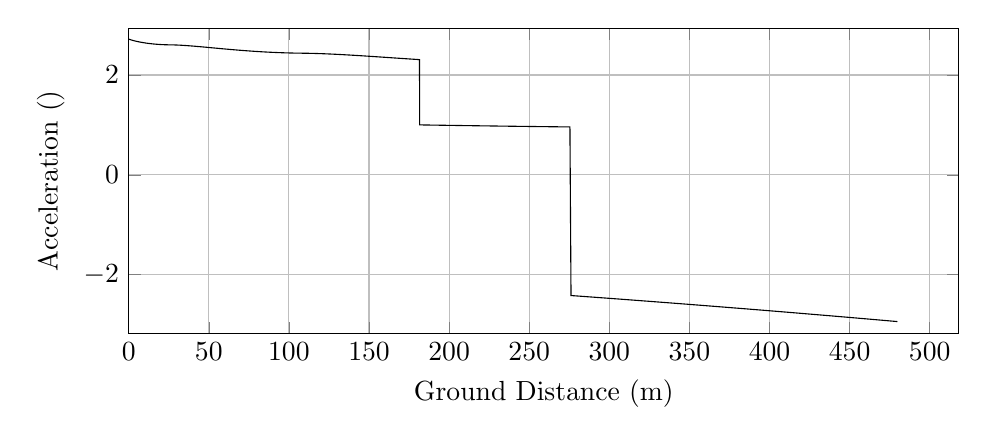
\begin{tikzpicture}

\begin{axis}[
width=\textwidth,
height=0.45\textwidth,
scaled ticks=false, tick label style={/pgf/number format/fixed},
xmin=0.0,
xmax=518.2299866992206,
xlabel={Ground Distance (m)},
xmajorgrids,
ymin=-3.1773545999999997,
ymax=2.9383329541999035,
ylabel={Acceleration ($\si{\meter\per\square\second}$)},
ymajorgrids
]

\addplot [
color=black,
solid
]
table[row sep=crcr]{
1.3603393307216043E-8	2.7206786612962066\\
3.0265395163403265E-7	2.7206786575478663\\
2.9593179127983543E-6	2.720678623102561\\
1.5392338359717934E-5	2.720678461954531\\
5.361280674027254E-5	2.720677966838565\\
1.6215010178508227E-4	2.72067656204086\\
3.7214145765703975E-4	2.7206738472617644\\
6.839954676020354E-4	2.7206698208009303\\
0.001098342709021993	2.7206644781690326\\
0.001609317716481928	2.720657898521556\\
0.0022198920000388346	2.7206500470445976\\
0.002878710694837372	2.7206415863366757\\
0.0036835072341781794	2.720631264662134\\
0.004557929017412697	2.720620065218509\\
0.005559798278933152	2.7206072508981105\\
0.006651227400597502	2.720593310307307\\
0.007795849738889277	2.7205787100180707\\
0.009067984722810115	2.7205625050930307\\
0.010453165799939174	2.720544884429202\\
0.011915708813158052	2.7205263052738617\\
0.013455030027058647	2.7205067774080813\\
0.015131183092671713	2.720485542905256\\
0.01690803412933615	2.7204630640878813\\
0.01873590105740728	2.7204399717842405\\
0.020713359121301934	2.7204150242262424\\
0.022777736728155237	2.7203890166149653\\
0.024960970145273077	2.720361550334686\\
0.02723428625014468	2.720332991183297\\
0.029610395797831278	2.7203031828656163\\
0.03204086105441677	2.7202727354797975\\
0.03462344565878624	2.720240428049145\\
0.037295727153354774	2.7202070461575243\\
0.040089145853872785	2.720172200927615\\
0.042950967781251806	2.720136553473475\\
0.04592022141655751	2.7200996205862893\\
0.04897301836205646	2.720061702748449\\
0.052130294957187476	2.7200225431846228\\
0.05542514139564195	2.719981736190481\\
0.05879722600804832	2.719940032970274\\
0.06231520981015182	2.719896588593282\\
0.06596261503753809	2.71985161218164\\
0.06964559414821356	2.7198062636261993\\
0.07347193989652406	2.7197592186945316\\
0.07736619052035826	2.7197114090939323\\
0.08137137577670908	2.7196623095742662\\
0.08545617869345057	2.719612307396395\\
0.08969468676038628	2.7195605001527836\\
0.0940095881391464	2.7195078372446053\\
0.09845059220533334	2.7194537156433602\\
0.10296315144049947	2.719398803650983\\
0.10759658895065366	2.7193425044674013\\
0.1123317495250277	2.719285055060655\\
0.1171874363557737	2.719226231512753\\
0.12217670360507671	2.7191658807659147\\
0.12726806426274867	2.719104388277655\\
0.13231647880291775	2.719043505591589\\
0.13765212084557643	2.718979255700906\\
0.14294844966167852	2.718915575612513\\
0.14834594087957392	2.718850776179469\\
0.1539671093411843	2.718783393554209\\
0.15968242883369804	2.7187149872467513\\
0.16555834796315422	2.718644767062395\\
0.17157514414202774	2.718572975126893\\
0.17760320215284392	2.7185011602885174\\
0.18370335474801935	2.718428598213908\\
0.18983540939776816	2.718355767994354\\
0.19621099073945342	2.71828016185121\\
0.20278841209744758	2.7182022845362246\\
0.20952923284938563	2.7181225994433653\\
0.21624967405074952	2.7180432810935136\\
0.22309476488450758	2.717962618703716\\
0.22992510727843934	2.7178822560654536\\
0.2371653034562048	2.7177972065765106\\
0.2442573187228817	2.717714030740942\\
0.25144286317780873	2.7176298902582934\\
0.2588001799723505	2.7175438743570046\\
0.2662612189130884	2.717456784348257\\
0.27386560463063747	2.7173681626444637\\
0.2815803271719757	2.717278399069807\\
0.28946218069394425	2.717186838600849\\
0.29753588720841584	2.717093202164077\\
0.3056643119969481	2.716999085151018\\
0.31376446154764137	2.716905447247142\\
0.322071411728719	2.7168095739864153\\
0.3303680011285137	2.7167139752329605\\
0.3389039548234316	2.7166157779269238\\
0.3474123396293025	2.7165180568217986\\
0.3561645174790815	2.7164176993305276\\
0.36525289600634137	2.7163136602552074\\
0.3742306244196095	2.7162110592727844\\
0.3835584127627333	2.7161046359512806\\
0.392806747202999	2.7159992963816517\\
0.40218604538039837	2.7158926432422206\\
0.4115907129344223	2.7157858796460443\\
0.42143744457304466	2.71567428647879\\
0.4310567075016639	2.71556545561893\\
0.4412814114336725	2.7154499724249304\\
0.4513051702487684	2.715336954190609\\
0.461412558308395	2.7152231867172496\\
0.47173637532167356	2.715107181729816\\
0.4821484569390513	2.7149903860087328\\
0.492985116277161	2.7148690397708313\\
0.5036221628177362	2.714750136897867\\
0.5142245311302887	2.714631824704451\\
0.5252888808291518	2.7145085711433863\\
0.5363145235987512	2.7143859638369863\\
0.5471208511184944	2.714266001569709\\
0.5585110457184732	2.7141397764842328\\
0.569849942463402	2.7140143406519304\\
0.5817265165330987	2.7138831906112504\\
0.5935668742733842	2.7137526762523763\\
0.6053719027871456	2.7136227833355733\\
0.6172343027602503	2.7134924902367645\\
0.629515267228629	2.7133578414420363\\
0.6417789549774502	2.713223625078407\\
0.6542768803188956	2.713087092614826\\
0.6669828212214572	2.7129485413260808\\
0.6796225285147333	2.712810963606792\\
0.6925094233679154	2.712670951020117\\
0.7056620711738308	2.712528314808269\\
0.7184715206768946	2.7123896541914156\\
0.731725241748566	2.71224644554528\\
0.7449880440563246	2.71210340227731\\
0.7586792333483576	2.7119560127494973\\
0.7725063377467813	2.71180744006777\\
0.7863894274138714	2.7116585464046254\\
0.8004504964383841	2.7115080279916457\\
0.8147129313117618	2.711355643498586\\
0.8293722635741907	2.711199319563237\\
0.8437954335339908	2.711045809353851\\
0.8580702287827062	2.7108941643141264\\
0.8726489666047585	2.7107395815891637\\
0.8875094051704782	2.71058231221187\\
0.9027740629895862	2.7104210779590776\\
0.9182163910703112	2.7102582871089913\\
0.93361566230532	2.7100962680430207\\
0.9491799633800446	2.7099328325529592\\
0.9646343064330896	2.7097708672969585\\
0.9803727456894022	2.709606245240436\\
0.9957421603273868	2.709445792888064\\
1.0116767859397604	2.7092797605173207\\
1.028041387324289	2.709109585047088\\
1.0443915011410971	2.7089398986479614\\
1.060796374175649	2.7087699812388033\\
1.0773229908740651	2.7085991418227273\\
1.093971735592782	2.708427381313938\\
1.1110062543639518	2.7082519927924293\\
1.127891796882146	2.7080784867552516\\
1.1451224507351285	2.707901789639987\\
1.1624801114435046	2.7077241500217113\\
1.180077727863539	2.7075444206861308\\
1.1978884766667508	2.7073628870065507\\
1.215488397439855	2.7071838674900413\\
1.23351701382096	2.70700086120692\\
1.2518199984626128	2.706815453946845\\
1.2704235066044305	2.7066273960882796\\
1.2892140278280424	2.7064378476887043\\
1.3075714306593595	2.7062530536699114\\
1.3266673518109293	2.706061226593331\\
1.3462106477188795	2.7058653259925807\\
1.365306294594515	2.7056743205573586\\
1.3852885894463176	2.7054748750159323\\
1.404835539176236	2.7052801958417234\\
1.4251192118409102	2.7050786164214466\\
1.445164519989187	2.7048798402486423\\
1.4656054698512246	2.704677582294032\\
1.4853522740259328	2.70448261320705\\
1.5051589726327936	2.7042874650304656\\
1.5255757775517242	2.704086734977351\\
1.5464367798307013	2.703882084832995\\
1.5673163741652552	2.703677701736183\\
1.5879032567231621	2.703476621174312\\
1.6091523485848285	2.703269524882243\\
1.6303162371862876	2.7030637127206134\\
1.6519474169970438	2.7028538211267294\\
1.673879209980242	2.7026414892001265\\
1.6955666802836635	2.702431991449334\\
1.7172271378534343	2.7022232168933176\\
1.7402832823543353	2.7020014942594512\\
1.7634396102400074	2.7017793281512494\\
1.7861669372425006	2.7015617813004402\\
1.8088678577734645	2.70134498175241\\
1.831824248135399	2.7011262418173425\\
1.855578771396016	2.700900422190558\\
1.878960729162178	2.7006786627687136\\
1.9033179534858085	2.7004481971762466\\
1.9273833213731866	2.700221034259217\\
1.9518510462308036	2.69999062125975\\
1.9761594732990155	2.699762252000519\\
2.000437267212291	2.6995347079709724\\
2.0252281699074732	2.6993029056239726\\
2.0498006073458734	2.6990736918319493\\
2.0745611186355752	2.6988432699762965\\
2.0997746990963106	2.6986091919427624\\
2.1260324099367294	2.6983660174624884\\
2.1515212193659616	2.6981305429210893\\
2.1771505246334	2.6978943421232504\\
2.2031842637813908	2.6976549974131148\\
2.230133398733474	2.6974078524356484\\
2.257053086628849	2.69716159885499\\
2.283795213136285	2.6969175806879333\\
2.311477064851834	2.696665625359551\\
2.3387199014446116	2.696418295414511\\
2.3662694524467227	2.6961688121763228\\
2.3937852540088533	2.695920264452572\\
2.4216520071021392	2.6956691844160687\\
2.4501931244916175	2.695412689733759\\
2.478927626230634	2.6951551292366664\\
2.506685441631536	2.6949069598473416\\
2.53537335014481	2.6946511285282604\\
2.5633350931805676	2.694402408668485\\
2.5917889242519685	2.6941499522401395\\
2.6208221472873374	2.693893017414193\\
2.649872764173903	2.6936365943995533\\
2.679661174525658	2.693374346647764\\
2.709174609939316	2.693115202410163\\
2.740029385016756	2.6928450029067674\\
2.770444625703795	2.6925793711374686\\
2.801129860621211	2.6923121002927015\\
2.8318827297715705	2.6920449607525097\\
2.862425967677578	2.6917803520588715\\
2.893259332541544	2.691513943438512\\
2.92412139403754	2.6912480008689297\\
2.955064430161417	2.690982073760627\\
2.986690331721131	2.6907110120079434\\
3.019183403261743	2.6904332863730254\\
3.0507201588152526	2.6901644753864344\\
3.0830332871979023	2.6898897995808344\\
3.1154603869692448	2.6896149168057812\\
3.148592095396281	2.6893348450572363\\
3.181936872739324	2.6890537678748103\\
3.214370607724433	2.68878113196698\\
3.247565473366384	2.6885028717129815\\
3.281695868027062	2.688217580965926\\
3.316494330618462	2.6879275486747067\\
3.3513055302544137	2.6876382569780937\\
3.3860303583611797	2.6873505222587717\\
3.421934361445942	2.6870538933091392\\
3.456235826539576	2.6867713320849385\\
3.490536654441657	2.6864895809370513\\
3.526257338581564	2.6861970179578334\\
3.561372823896762	2.6859102537028257\\
3.5967906564503185	2.685621861580385\\
3.632682576242373	2.6853304665721813\\
3.6701261071689295	2.6850273896113928\\
3.707701291513044	2.684724181446221\\
3.7452745323452916	2.684421920005274\\
3.78256482255855	2.6841228504923897\\
3.8208821591411084	2.6838164893445455\\
3.8590337549211444	2.6835124003534068\\
3.89695718563138	2.683211061596486\\
3.9351036745073964	2.6829088826731304\\
3.9736642086653067	2.682604369291303\\
4.012189127077221	2.6823010815538098\\
4.05156219172609	2.681992087170766\\
4.090290786278251	2.68168910267706\\
4.129291984889424	2.681384935049498\\
4.1680648628189925	2.6810834879059993\\
4.207805169621487	2.680775486920913\\
4.248168240749736	2.6804636570116616\\
4.288797880674668	2.6801507780724796\\
4.32990243544832	2.6798352683149327\\
4.371428084678056	2.679517569343126\\
4.41247037137882	2.6792045933860082\\
4.453879445321437	2.678889847978703\\
4.49524783594077	2.678576437358818\\
4.537299342543221	2.678258896831071\\
4.580546125800922	2.6779334244468345\\
4.622914948498307	2.6776156299698934\\
4.66640222022569	2.677290542721363\\
4.709294790611851	2.6769709837785767\\
4.752417172855319	2.6766507912603412\\
4.796155651503765	2.6763271235040342\\
4.8408754796551925	2.675997332877057\\
4.884850997559644	2.675674149017089\\
4.928651138956553	2.6753533505106946\\
4.972831351372241	2.67503087161995\\
5.017331702752941	2.6747071708341474\\
5.0632326321008225	2.6743744487516317\\
5.108452384314601	2.6740478173091553\\
5.1536021218025905	2.673722827898078\\
5.199057463234675	2.673396780336388\\
5.244479287100011	2.6730721120468193\\
5.292293005248643	2.6727315710052038\\
5.338096108273211	2.6724065220089717\\
5.3857492800262605	2.6720695551603235\\
5.433816232374781	2.67173090807856\\
5.480691139018431	2.6714018586329598\\
5.529685763332537	2.6710591891667725\\
5.578612887337309	2.6707182708184654\\
5.626451501744754	2.6703861671011913\\
5.674834544150631	2.6700515151935553\\
5.7252048440372345	2.669704427524425\\
5.77422346516266	2.6693679305667333\\
5.8255152536468575	2.6690171710063213\\
5.874338256646894	2.6686845632866065\\
5.922631450506765	2.668356777034105\\
5.972682300942642	2.6680183272823603\\
6.022535370757359	2.6676824906956176\\
6.074394648705015	2.6673344842246873\\
6.124928192945902	2.666996687642375\\
6.176798284396469	2.6666512989764355\\
6.229620191179453	2.666300963486928\\
6.282808156696705	2.665949612003093\\
6.334658925277093	2.665608451405185\\
6.388041948821611	2.6652586030534966\\
6.440558117792513	2.6649158095309824\\
6.494960924490993	2.664562131646191\\
6.550441697666145	2.664202938277337\\
6.6042098433346865	2.6638562643536536\\
6.658315220792536	2.663508832144151\\
6.712335084641163	2.663163359917985\\
6.766674450459032	2.662817260436796\\
6.821537769035839	2.6624692583213525\\
6.876851268142238	2.6621198535092523\\
6.933661362437203	2.6617625068113426\\
6.989261882852809	2.6614142454795733\\
7.046240323930029	2.6610588624640483\\
7.102786137967051	2.6607076814481774\\
7.1603789170469145	2.66035153122335\\
7.21785165788507	2.6599976588428076\\
7.277487498606879	2.659632082256504\\
7.334984696129153	2.659281165977336\\
7.393362172524569	2.658926427334934\\
7.452416393609804	2.658569158697232\\
7.511934748111884	2.65821068542132\\
7.572557225035805	2.6578472095603285\\
7.63202184821041	2.6574922841322914\\
7.69294899409779	2.657130274209857\\
7.752675521499926	2.656777007005755\\
7.814488876138199	2.656413067005313\\
7.8763528528159785	2.6560505226767974\\
7.938149975125226	2.6556900545173407\\
8.001193143199774	2.65532404532037\\
8.064554080136986	2.654957941394265\\
8.12686567918485	2.654599604470868\\
8.189637855946287	2.654240320036407\\
8.252542711798306	2.653881981811166\\
8.315859663763469	2.6535230130597807\\
8.380006162932737	2.653161090486292\\
8.444702551512929	2.6527978411523154\\
8.509501986620958	2.6524357933385767\\
8.57387297516295	2.6520778958356077\\
8.63887365699837	2.6517182663260552\\
8.70727085773305	2.6513417562064703\\
8.772937378995405	2.650982114230926\\
8.839192134487615	2.650621066200708\\
8.905815929161982	2.6502598384638087\\
8.97209054442786	2.649902318438188\\
9.039019026885107	2.6495431001632594\\
9.107371801018814	2.6491781267509182\\
9.174915633685494	2.6488193404634632\\
9.243868961478196	2.6484549743174144\\
9.312440636565494	2.6480945280533144\\
9.381784695008012	2.64773194388124\\
9.4513167952828	2.647370309297383\\
9.52142787533916	2.647007615113754\\
9.591425279059166	2.6466474560144393\\
9.662230428326719	2.646285111993561\\
9.734225879912522	2.6459187011004124\\
9.806441602430919	2.645553211506668\\
9.878483835105534	2.6451906297210153\\
9.951807209049782	2.644823673290537\\
10.023539677466466	2.644466694479261\\
10.096057433179052	2.6441078259737703\\
10.168262179450682	2.643752514614059\\
10.241274410624943	2.6433952591641816\\
10.31479015323385	2.6430375937029646\\
10.390063469390178	2.6426735041074956\\
10.465012435634037	2.642313112770144\\
10.540639152111389	2.6419516075562184\\
10.617644389866598	2.6415857179533573\\
10.692945462162374	2.641230068796194\\
10.770083295573727	2.6408679330963514\\
10.846726862770723	2.6405103027817125\\
10.924657809445929	2.640148889613137\\
11.00265335491597	2.63978941352116\\
11.081827589833612	2.639426784384952\\
11.159134327011738	2.639074915846357\\
11.239152720133266	2.638712992829407\\
11.317028257314295	2.638362987873357\\
11.396413369884492	2.6380084493978577\\
11.477655063362434	2.6376479632370904\\
11.556958506738276	2.637298355398907\\
11.637325199769407	2.6369463471769103\\
11.717754170658207	2.6365963621380466\\
11.799819443100102	2.63624161502403\\
11.881986970940797	2.635888803104182\\
11.964394119506721	2.635537342147723\\
12.046263329632716	2.6351905264087696\\
12.130282587748898	2.6348370295798214\\
12.213721087180826	2.634488399852607\\
12.295868535962462	2.634147514971435\\
12.380692430046633	2.633797961762415\\
12.46470288467437	2.633454193025379\\
12.550384439940181	2.6331060699957733\\
12.635259749824865	2.6327636863268946\\
12.72144647897981	2.63241851197907\\
12.80741162779486	2.632076724560571\\
12.892901506907108	2.631739293069713\\
12.977815703098727	2.6314065594474236\\
13.06483740414145	2.631068066500708\\
13.151922956503014	2.630731848075155\\
13.240589045456186	2.6303921107814636\\
13.329911181207382	2.6300524853438656\\
13.417306166647748	2.6297227285188542\\
13.507103029723119	2.6293865171984176\\
13.595986036712912	2.6290563212297444\\
13.687453390597003	2.628719208644787\\
13.779071846306106	2.6283842583240453\\
13.872694200363323	2.628044782677631\\
13.963504841252302	2.627718197075353\\
14.056146454975131	2.6273877509805974\\
14.14918846816267	2.6270586358496457\\
14.24332804549016	2.626728442147807\\
14.339261112049854	2.626394848369028\\
14.431091301610323	2.6260782450404214\\
14.524174633942373	2.625760029885301\\
14.618760344060338	2.6254394620095756\\
14.714801736988441	2.6251168208410443\\
14.809763128346521	2.624800631225546\\
14.903412319659619	2.624491550424864\\
15.001392651385917	2.6241710768230613\\
15.098055049922994	2.6238578111877793\\
15.196870856960619	2.623540530466907\\
15.29477342819068	2.6232291262965033\\
15.39265348361268	2.6229207128263496\\
15.490487151984588	2.6226153517984745\\
15.588146853189365	2.6223134213572887\\
15.687961867268871	2.622007798116239\\
15.78650099417861	2.621709016912882\\
15.886965864441798	2.6214073886179268\\
15.98755318095926	2.6211084084990697\\
16.088470385762115	2.6208114696538525\\
16.190536977381747	2.620514216689597\\
16.292466610053154	2.6202204307907557\\
16.396448349404487	2.6199238784454053\\
16.497808944935016	2.6196378512110607\\
16.600551072850564	2.619350987382476\\
16.70575139586156	2.6190604431728257\\
16.81134459259622	2.6187720413883815\\
16.917616592554033	2.618485038902799\\
17.023477948501657	2.6182023789046003\\
17.12904978140002	2.617923694814939\\
17.2354081519902	2.6176461576139998\\
17.340772011500363	2.617374394528855\\
17.448391076872838	2.6171000698358444\\
17.5571980918308	2.6168260499237155\\
17.66615596614949	2.616554996724549\\
17.774685459577412	2.6162883270448347\\
17.884986575683584	2.6160206855256734\\
17.99552903728076	2.615755866553193\\
18.108708479124623	2.615488253160013\\
18.219646262474413	2.615229387506168\\
18.332680252669796	2.6149691286881325\\
18.445061806396694	2.614713860659559\\
18.556709221711323	2.614463693032193\\
18.668884868236475	2.614215776215975\\
18.78204748093455	2.613969154620711\\
18.895704562363058	2.6137249583668334\\
19.008928234289563	2.613485172303819\\
19.124320907419907	2.613244353656583\\
19.24105855786135	2.6130043738052313\\
19.355116774466126	2.6127734319677236\\
19.470462572962035	2.6125434196100388\\
19.58492145104516	2.612318679974858\\
19.704921229319112	2.6120867966885672\\
19.821259826163917	2.611865627200067\\
19.941172080873493	2.6116414010344053\\
20.06078806851737	2.611421496185992\\
20.177423389922623	2.6112106825265204\\
20.297621170678	2.6109971487959625\\
20.420129559802255	2.610783382130866\\
20.54164670774839	2.610575194034384\\
20.661905244258705	2.610372924043535\\
20.784301666224792	2.610170888533478\\
20.904244540623438	2.609976639812995\\
21.028114340450195	2.609779901698209\\
21.148300883955606	2.609592760781454\\
21.270875420257596	2.6094056910343086\\
21.39299406946177	2.6092231107132005\\
21.513793771711654	2.6090462163639767\\
21.637476506915142	2.608868915612577\\
21.759279707150128	2.6086980705627534\\
21.88493035745168	2.6085257282674936\\
22.009809790007786	2.6083583553647216\\
22.13620730934617	2.6081929065801015\\
22.263515470260465	2.6080302793333896\\
22.393040471753594	2.607868941280868\\
22.520519759768852	2.6077141976473044\\
22.648852607677917	2.6075624600019314\\
22.775118904521122	2.6074171120820617\\
22.903136237443974	2.607273732646484\\
23.03176118514304	2.6071337008954343\\
23.162501585272054	2.6069954916827385\\
23.294719932439598	2.606859937497086\\
23.427108470281937	2.6067284454088675\\
23.558693146983046	2.606601940003137\\
23.687077503630363	2.606482524014279\\
23.817949558665852	2.6063648614675117\\
23.948210788889448	2.6062518140947457\\
24.076877750667826	2.6061441212975813\\
24.21019765060587	2.606036685397494\\
24.3450673155249	2.605932287377364\\
24.477101355489637	2.6058342488821085\\
24.60984760833776	2.605739823492751\\
24.7468403923846	2.6056467196227446\\
24.882807251950062	2.605558661740309\\
25.017167332957627	2.6054758883508313\\
25.153910941279605	2.6053959660017787\\
25.289629217480112	2.6053209394618975\\
25.425306692573436	2.605250202063977\\
25.56229499031975	2.6051830973115537\\
25.70075944713021	2.605119664500041\\
25.83724158708921	2.605061452167142\\
25.975209935932874	2.605006945543712\\
26.003074150630965	2.604996465857483\\
26.020759913393235	2.6049899063023956\\
26.030714598210515	2.604986245585444\\
26.05840292223249	2.6049761825189828\\
26.06133765907019	2.6049751261727927\\
26.064285136409026	2.6049740672190262\\
26.066337724202356	2.604973330947354\\
26.068175973881182	2.6049726717880395\\
26.06984477238784	2.604972072546399\\
26.077831036047115	2.604969193304239\\
26.10345636352254	2.604959826557275\\
26.16716044512971	2.604935696636902\\
26.297541524199602	2.604882582063598\\
26.42722303713863	2.604824833845874\\
26.5559280656694	2.604762729734616\\
26.686097387723095	2.6046951240870673\\
26.817793678842584	2.6046218784664346\\
26.949416928520378	2.6045438626963486\\
27.080440623797912	2.6044614849705248\\
27.215491080424528	2.604371711442483\\
27.34795890217076	2.6042789179214214\\
27.48215578365496	2.6041801903944934\\
27.616696052324144	2.6040764988267338\\
27.75271189183823	2.6039669358068878\\
27.888759310501555	2.6038526466269865\\
28.023839122857026	2.60373457871965\\
28.16136324828667	2.6036097347187157\\
28.298355249881332	2.603480779773336\\
28.435282447697354	2.603347363417516\\
28.573941346212784	2.603207712242628\\
28.713752690797136	2.603062327801072\\
28.852681198061333	2.6029133732207983\\
28.992471984120606	2.6027590381432235\\
29.133421724605903	2.6025989580439326\\
29.275199211812186	2.6024334748055615\\
29.416225289053614	2.602264487584124\\
29.55783477945603	2.6020904638423383\\
29.701838356359822	2.6019091010670348\\
29.846633046394217	2.601722332586834\\
29.99013730470424	2.6015329260160254\\
30.132492646908446	2.6013408617739424\\
30.277395768405135	2.6011411490535545\\
30.422188862471998	2.600937402849355\\
30.56637548064623	2.600730410308623\\
30.711944318924978	2.6005173409279383\\
30.8573377156769	2.600300480843197\\
31.006558691603843	2.6000737648824686\\
31.153907258126303	2.59984583014083\\
31.30257185742142	2.599611825960162\\
31.4510947803754	2.5993740568584256\\
31.602595106592503	2.599127473961757\\
31.755261577184278	2.5988749186996953\\
31.906398416479824	2.5986209245321756\\
32.05599258457312	2.598365690945168\\
32.20952926265106	2.598099824891996\\
32.360097140052986	2.59783531374599\\
32.51218835243483	2.5975643770630965\\
32.664721606344784	2.597288924507674\\
32.82129760777845	2.59700234643684\\
32.97669884718651	2.5967141455121885\\
33.13118849606322	2.5964239666121385\\
33.288837444683736	2.596124141007718\\
33.44405554194745	2.5958253313356394\\
33.60015866510213	2.59552126423476\\
33.756686089655645	2.59521284804464\\
33.91694077595571	2.594893491070727\\
34.074326811338736	2.594576365075885\\
34.23252403098988	2.5942541792298783\\
34.392884168270385	2.5939241396518096\\
34.554266068788166	2.593588548636937\\
34.71363140184178	2.5932538115207127\\
34.87649332318763	2.592908357922452\\
35.03746231629111	2.5925636252736934\\
35.19990059234286	2.592212481401056\\
35.3627309111595	2.5918572538216775\\
35.5271254050015	2.5914953825208134\\
35.69149466827288	2.5911303760815123\\
35.85508342515686	2.5907639894772565\\
36.017180984292054	2.590397931582352\\
36.182222084544165	2.5900222000957323\\
36.34861175093968	2.589640361269958\\
36.514166392421686	2.589257465430392\\
36.68083924241549	2.5888690407516313\\
36.845526722294395	2.5884823945483877\\
37.01328249159678	2.58808568617886\\
37.18160982421668	2.587684779048817\\
37.35136716620059	2.5872776308265406\\
37.51969289597564	2.5868711570289102\\
37.689710015857784	2.586457862001348\\
37.860394939778416	2.5860402290187876\\
38.02805196867635	2.5856274069225176\\
38.19868492919754	2.5852046641593693\\
38.37343039987371	2.5847690739970304\\
38.54685896696101	2.5843341589437943\\
38.71934233168869	2.583899089049461\\
38.8915617091798	2.5834622227014767\\
39.062305982326905	2.5830267178960575\\
39.23847188392709	2.5825749507861113\\
39.411511502305984	2.582128843751896\\
39.585172817779906	2.5816788341031485\\
39.760693028009456	2.581221715331284\\
39.9373134006328	2.5807594546179793\\
40.113617753210534	2.580295792292225\\
40.29094651898711	2.5798272385973133\\
40.468149621311596	2.5793568640609754\\
40.64593210594187	2.578882837045067\\
40.82431302355218	2.5784051336362657\\
41.00141330502653	2.577928844765018\\
41.17957893337042	2.577447711440911\\
41.359761290266974	2.576959159908581\\
41.53889737920997	2.5764715258014226\\
41.72013507746885	2.5759762699463096\\
41.899395797464194	2.5754845813065144\\
42.081280067494475	2.574983877308929\\
42.265315320939635	2.574475433596758\\
42.44531744651641	2.5739764081138246\\
42.62715102096499	2.5734706185694742\\
42.81120266452106	2.572956977963316\\
42.994164503876235	2.5724447468852603\\
43.17799769459725	2.5719284820894615\\
43.36154361404071	2.5714114735636295\\
43.54597437124032	2.5708904557742125\\
43.73158498218817	2.570364613472675\\
43.91737182308138	2.569836817130298\\
44.1050494697441	2.5693022153985066\\
44.293574236233	2.5687637938290475\\
44.47888581456586	2.568233217366008\\
44.66456251492659	2.56770031290059\\
44.85170130968709	2.5671619544796576\\
45.037822074257164	2.5666253131937316\\
45.22676109993536	2.566079351527528\\
45.41612608476639	2.5655309928311034\\
45.604812217355104	2.5649834795818123\\
45.79422221198037	2.5644327816257144\\
45.98724683785376	2.5638704982109193\\
46.17830917717477	2.5633129020510665\\
46.36786657808848	2.5627587260007036\\
46.55935209439748	2.5621979696912565\\
46.75090376717816	2.5616361102767\\
46.94233405988251	2.5610737370838272\\
47.13714948644359	2.5605005660882156\\
47.33387512950824	2.559920942035922\\
47.53043319838464	2.559341016085903\\
47.72298239739284	2.5587721852277925\\
47.919150009665316	2.5581919576628076\\
48.113386178114425	2.5576167774288168\\
48.311024807628144	2.557030880297275\\
48.508886059616145	2.5564437135036124\\
48.70490444306449	2.555861451460194\\
48.90290918859142	2.555272756407139\\
49.09959709013448	2.5546874831690767\\
49.2970021191946	2.554099617958525\\
49.49532701226336	2.5535085875213586\\
49.693780717172615	2.5529167818555347\\
49.89506320355713	2.5523161771326155\\
50.096719083698545	2.5517141278441926\\
50.29606895218413	2.5511186737396656\\
50.497598474286534	2.550516452001548\\
50.700304208193415	2.549910490324689\\
50.90342397924904	2.5493031000410458\\
51.10460922167407	2.5487013408370585\\
51.30752217039489	2.5480942934029542\\
51.51010619677311	2.5474881432730276\\
51.713602501430145	2.546879210211035\\
51.91843850546792	2.546266248332386\\
52.121089026646246	2.545659839831946\\
52.32561402362407	2.5450478687524436\\
52.53192272805477	2.5444306412072404\\
52.7387030603267	2.543812117268339\\
52.944027344085896	2.5431980948169493\\
53.154073670302836	2.542570135158037\\
53.36143953271798	2.5419504044032433\\
53.571009444677685	2.541324336833787\\
53.77799762982136	2.5407062605659156\\
53.98785945427545	2.5400799181832214\\
54.196157549666225	2.5394585875123497\\
54.40718762937186	2.5388294894484362\\
54.616887598525366	2.538204768354279\\
54.826875464266934	2.537579631685529\\
55.04038432082807	2.5369444978423\\
55.25438844036796	2.5363084127457762\\
55.46695867894975	2.5356771378333054\\
55.68088820258777	2.53504240855004\\
55.895144656119854	2.5344073252295782\\
56.109028395418505	2.5337739915506914\\
56.326262430904194	2.533131427269357\\
56.542089933321776	2.5324937421273432\\
56.76060076462056	2.5318488889481365\\
56.97729209122687	2.53121019040462\\
57.19579178641709	2.530566982970221\\
57.41258192878804	2.5299296520756522\\
57.634093277561306	2.5292793396004543\\
57.85395098827546	2.528634808787415\\
58.07448819514299	2.527989242816962\\
58.29446478173499	2.5273463011751724\\
58.51588770709739	2.526700152443185\\
58.73757884137123	2.5260542747954213\\
58.96020041504734	2.5254067756961724\\
59.18267120664716	2.524760833573292\\
59.405949655899676	2.5241136983448893\\
59.63089974393067	2.523462913015166\\
59.8562534200115	2.522812190429593\\
60.084134136581554	2.522155451171125\\
60.30833762904015	2.521510593077889\\
60.53504725699203	2.5208598484686284\\
60.763693228044005	2.520204919132267\\
60.99075593752245	2.5195559165490664\\
61.21765734918529	2.5189087867059206\\
61.44713116872772	2.5182557820175218\\
61.6738048454246	2.51761221451096\\
61.90668490141796	2.5169525728970683\\
62.13729676517957	2.5163009271692243\\
62.36629463006145	2.515655414734929\\
62.596359157213186	2.5150084986834154\\
62.82836101237727	2.5143577875240695\\
63.059723307860466	2.513710547655892\\
63.292774394726166	2.5130603018722466\\
63.52608473446321	2.512411085168192\\
63.75973181411028	2.511762713251054\\
63.993403028653574	2.5111160820431335\\
64.23068717493263	2.51046132747829\\
64.4710952259949	2.5097999046051767\\
64.70858695601663	2.5091484588673003\\
64.94894296164699	2.5084911580978195\\
65.18738841845183	2.507841096140126\\
65.42661162888535	2.5071909536442867\\
65.6659442133793	2.506542582107792\\
65.90899583190168	2.5058862766024292\\
66.15068261105333	2.505235819878556\\
66.39533053734849	2.5045796148039337\\
66.6378997293487	2.503931215046631\\
66.88158418814953	2.5032820928672956\\
67.12390450547147	2.5026388721469575\\
67.36840986262189	2.501992166121669\\
67.61550053739396	2.5013410071229005\\
67.86097385246623	2.5006965071294838\\
68.10985741250389	2.500045515162805\\
68.35582503705197	2.4994046078616874\\
68.60464259362828	2.4987587826507225\\
68.85450289166104	2.4981128115549627\\
69.1042877596268	2.497469622399734\\
69.35837572129628	2.4968180291693622\\
69.61150655903072	2.496171596673576\\
69.86289252102952	2.4955323152395783\\
70.11686816207683	2.494889197346831\\
70.37125759672608	2.494247823299956\\
70.62480458144697	2.4936113746348187\\
70.88045310059783	2.4929725036104173\\
71.13526709211152	2.4923385896920447\\
71.3947754873567	2.4916959652598996\\
71.6534187996231	2.4910584844101127\\
71.91450497256008	2.490418042920515\\
72.1716184080999	2.4897903719922825\\
72.43269265097052	2.489156124566061\\
72.69331619504374	2.488526100829059\\
72.95563200429567	2.4878951633499824\\
73.21686762735783	2.4872700118660225\\
73.48161420086069	2.486639724524867\\
73.74261486234883	2.4860215932579317\\
74.00755043430098	2.485397450822168\\
74.27511769675363	2.484770511126462\\
74.54487113507057	2.484141930683326\\
74.81568229507957	2.4835144223616146\\
75.08274085953312	2.4828990994561133\\
75.35421836228127	2.48227716702688\\
75.62798354862159	2.481653660677785\\
75.89909469738902	2.4810398475160156\\
76.17008148658607	2.48042996336775\\
76.44269151183332	2.479820124431633\\
76.71571902594138	2.4792130884926618\\
76.99340852183178	2.4785995427236145\\
77.27004772085374	2.477992202674521\\
77.54832408953641	2.477385199695421\\
77.82592519882277	2.4767836170636297\\
78.10358246820337	2.4761858750642443\\
78.38556010231375	2.475582906634508\\
78.66911430382748	2.474980726291445\\
78.95399134982776	2.4743799558012434\\
79.23667137346987	2.4737880172861093\\
79.518907793654	2.4732011984459694\\
79.80555437718249	2.4726095145346116\\
80.09150103324356	2.4720236154797126\\
80.37928873457926	2.4714383390733685\\
80.66871996946384	2.4708541852254573\\
80.95967699414447	2.470271483310257\\
81.25093884305389	2.46969273945421\\
81.54344278085921	2.4691161457324657\\
81.8358102960415	2.468544463485582\\
82.13087592438694	2.467972229211356\\
82.42794520371837	2.4674009209561696\\
82.72842933895026	2.466827975237794\\
83.0269479931649	2.466263704519231\\
83.32974506690314	2.465696381887148\\
83.62964811531441	2.465139497828961\\
83.92951211009506	2.4645876948518985\\
84.2339319847595	2.4640326486757456\\
84.53715838283946	2.4634849446277407\\
84.84105485927768	2.4629412204221763\\
85.14845677960258	2.4623965277685977\\
85.45530133949276	2.461858159152909\\
85.76249773413784	2.4613245309354017\\
86.07201271349416	2.4607923136600105\\
86.38432073331904	2.460260843847024\\
86.69710203601804	2.4597341734019187\\
87.01172103282082	2.459210084155634\\
87.32669099459858	2.4586911288738795\\
87.64517025121202	2.4581722263462886\\
87.96158123090564	2.4576625205007074\\
88.2775814178033	2.4571592893344167\\
88.60068374099544	2.456650771249656\\
88.92068281935622	2.4561531565110357\\
89.24207276858638	2.4556594246506958\\
89.56578933015979	2.4551682597665963\\
89.88760090270688	2.4546861104221787\\
90.2141410750086	2.454203135124871\\
90.54066676000363	2.453726501259575\\
90.86727570256076	2.453256084169672\\
91.19715108614633	2.4527874130189637\\
91.52744226539704	2.452324662124046\\
91.85639956214655	2.451870271480665\\
92.19095740864739	2.4514148053995646\\
92.52827526888461	2.4509623982187643\\
92.8674718219292	2.4505143893221693\\
93.20307982994817	2.45007796351259\\
93.5374944579234	2.4496498757217147\\
93.87598013161067	2.449223490262768\\
94.20917297854535	2.448810580306356\\
94.55043409744499	2.4483946888723898\\
94.89132963816093	2.4479863478956343\\
95.23083207736542	2.447586748328506\\
95.57395676502793	2.4471900719482775\\
95.91421223354143	2.4468038617271874\\
96.25656086122288	2.446422475256802\\
96.60012122339742	2.4460470135485375\\
96.94166303707107	2.4456809955647865\\
97.28627502929558	2.445319015713345\\
97.62906225262071	2.4449662694279697\\
97.97125437026659	2.444621427786916\\
98.31201772458999	2.444285279829848\\
98.65627175165852	2.4439530523110857\\
99.0012536203806	2.443627560750417\\
99.35020029285332	2.4433059171884537\\
99.69475740907401	2.4429958218600083\\
100.04053871990226	2.4426921324246553\\
100.38598466112728	2.442396260584223\\
100.72867962848932	2.4421101874466906\\
101.07385499050397	2.441829549808382\\
101.41864366415388	2.441556759554321\\
101.76305460768467	2.441291796930587\\
102.11068844700483	2.441031997901126\\
102.45638678530696	2.440781272232182\\
102.79841653079728	2.440540704148865\\
103.14087212494877	2.4403073190123745\\
103.48486473791618	2.4400804356214234\\
103.82875595362174	2.4398611934533667\\
104.17244250654872	2.4396496596833757\\
104.51168383396202	2.4394483022733917\\
104.85986244643053	2.4392493381386604\\
105.204587526496	2.4390600412341765\\
105.54754777175077	2.4388793212149045\\
105.88797456536247	2.4387074512981224\\
106.23280177240994	2.4385410036507142\\
106.57515110440406	2.4383833730122237\\
106.91603555764121	2.438233972158936\\
107.25729565943405	2.438091968620996\\
107.598830149446	2.437957436469797\\
107.93686571059558	2.4378317650253747\\
108.27485499032852	2.437713563105536\\
108.28839963475954	2.4377089816955086\\
108.30004107281309	2.4377050536118228\\
108.30931238392475	2.4377019315951367\\
108.31701527366243	2.4376993419985693\\
108.32505202073054	2.4376966442959924\\
108.33865239118708	2.4376920757662077\\
108.35091925899997	2.437687941820947\\
108.39508146726081	2.4376729541898428\\
108.52984553865659	2.4376262051439177\\
108.79919793188978	2.4375282156126596\\
109.105233418432	2.4374095713382307\\
109.41485218466596	2.4372816990329653\\
109.72257164661937	2.43714687531413\\
110.0321119530083	2.4370035496994156\\
110.34145354075926	2.4368526728261344\\
110.6534776714839	2.436692824043207\\
110.9711963390063	2.4365222289562025\\
111.28851843247409	2.4363440420862066\\
111.60893519474632	2.4361562847481197\\
111.92798394282838	2.4359615896983087\\
112.24770070245137	2.435758820731417\\
112.57243448635171	2.4355450966094914\\
112.89480865389396	2.4353252588963645\\
113.22000325235314	2.4350958414002974\\
113.54885709436653	2.4348561065866923\\
113.8770619430189	2.434609173215901\\
114.20946079557197	2.4343513587107797\\
114.54107775051554	2.4340864891862495\\
114.87787736567807	2.4338097352623684\\
115.21564640021248	2.4335244348530267\\
115.55522358014255	2.433229873390224\\
115.89667501383605	2.4329259578067397\\
116.23992536102014	2.4326127213255626\\
116.5847156213415	2.432290379243784\\
116.92791619634093	2.4319619499620595\\
117.27517516660399	2.4316220384861005\\
117.62420948631524	2.431272780277488\\
117.97391125359778	2.4309152972309223\\
118.32673409155768	2.430547052323676\\
118.68227803698588	2.430168369963023\\
119.03889207644076	2.4297809832770483\\
119.39651249432902	2.429384992014123\\
119.75508651978987	2.4289804895119858\\
120.11314113323388	2.4285692199538316\\
120.47404637453192	2.428147337094468\\
120.84098349318353	2.4277109488262347\\
121.20490030977416	2.427270827669072\\
121.57328571082118	2.426817972786023\\
121.94079100066682	2.4263589516450033\\
122.31015242291167	2.425890417592221\\
122.68267403243519	2.425410670298904\\
123.05346836176264	2.424926062633208\\
123.42835733050345	2.4244290188823996\\
123.80350972566416	2.4239245961583267\\
124.1783235941891	2.4234137066845376\\
124.55244040146786	2.4228969673348413\\
124.92576251095704	2.4223746517122615\\
125.30489170817492	2.421837488041481\\
125.68146781278597	2.4212973337292256\\
126.06139977608174	2.4207457916277306\\
126.44502763856761	2.420182285371527\\
126.82695116404781	2.4196147964977337\\
127.206716044588	2.4190441968488976\\
127.59262031825523	2.4184580188810942\\
127.97077035934353	2.417877503078614\\
128.3546122768156	2.4172821552332753\\
128.73724861847296	2.4166826630374114\\
129.12002064685282	2.4160770463275636\\
129.50086700331673	2.4154687022193597\\
129.8837789976152	2.414851346010222\\
130.26783132854348	2.4142264916091953\\
130.651936341801	2.413595975813511\\
131.03747321415574	2.412957595804226\\
131.42280335891803	2.4123141313718692\\
131.80875442588928	2.411664284079559\\
132.19322104975072	2.4110117078378126\\
132.5798881414172	2.410350224396862\\
132.96215446290768	2.409691259338784\\
133.34488286943906	2.4090265945736995\\
133.7276157954845	2.4083571021251338\\
134.11532375481391	2.407674080588845\\
134.50135826447365	2.406989268013292\\
134.88604120201086	2.406302234909834\\
135.26955723714872	2.4056127810566927\\
135.6512109336153	2.4049222924372256\\
136.03464327936558	2.40422426529637\\
136.41686422877552	2.4035242144151487\\
136.79904942565338	2.4028200875141854\\
137.18004416157777	2.402114110924786\\
137.56399804528928	2.401398646520869\\
137.94515347717788	2.400684498489757\\
138.32982901897384	2.3999598952989585\\
138.7128522769853	2.399234629307342\\
139.09597564505458	2.398505481924219\\
139.48002685240425	2.3977709392261835\\
139.86309097971855	2.3970347399419127\\
140.24727738828375	2.396292903294329\\
140.6317581809211	2.3955470832041623\\
141.01585725597846	2.3947986662434966\\
141.3998433603236	2.3940472083670095\\
141.7841907991213	2.393291850794408\\
142.16710976343057	2.392536195828421\\
142.55205218648928	2.3917734955203658\\
142.9364233092117	2.3910089444426257\\
143.32169829765928	2.390239674944902\\
143.705984531242	2.3894695365580034\\
144.08985428249122	2.3886974667514584\\
144.47683600496026	2.387916408652118\\
144.86371007721533	2.3871328975357295\\
145.24772592056325	2.3863526020597376\\
145.63047789911974	2.385572389946076\\
146.01273254364395	2.384790780760845\\
146.39725173307323	2.3840021753782183\\
146.77966503747456	2.383215599586898\\
147.16478130736948	2.3824212209002393\\
147.54689717238745	2.381630869102909\\
147.93097497792814	2.3808343517343653\\
148.31499270913332	2.380035908616705\\
148.69957284780122	2.3792343033244103\\
149.08709998577143	2.3784246003791054\\
149.47129868208145	2.377619975755045\\
149.8546635899794	2.376815295395449\\
150.23801379389647	2.376008905260921\\
150.62200569343076	2.37519947915814\\
151.00751012558203	2.374385226029803\\
151.3946455315429	2.373565934584871\\
151.77987817077866	2.372749143111779\\
152.16505704867353	2.3719310003601963\\
152.55112759502248	2.3711095505099173\\
152.93964308710213	2.370281527621655\\
153.32507651584535	2.3694587708503905\\
153.71174813432617	2.3686321233352805\\
154.10000329570875	2.367800888914693\\
154.48914219495543	2.366966610175619\\
154.8788297075107	2.366130054853258\\
155.26820650111182	2.365293121841945\\
155.6562915247282	2.364457980569835\\
156.0441896603637	2.363622312599576\\
156.4348678136667	2.362779770569401\\
156.82082928279863	2.3619465809003035\\
157.21071017196311	2.3611041555010726\\
157.60005066896917	2.360262172782705\\
157.99004282467217	2.3594181063852853\\
158.3808231456182	2.3585717087559077\\
158.77280374485122	2.3577221340717758\\
159.16384255262415	2.3568740754878803\\
159.55370941764693	2.3560280866240024\\
159.946071590523	2.3551762575385133\\
160.33752628124114	2.354326022930576\\
160.73008933968674	2.3534730536514\\
161.12428312893906	2.352616260804793\\
161.5185576482712	2.351759060855163\\
161.91431288671106	2.35089845795311\\
162.3096877663487	2.35003854728694\\
162.70613442998513	2.3491762188949528\\
163.1032465869576	2.348312404430774\\
163.50039135636405	2.3474485286109577\\
163.89625578410926	2.3465874947997296\\
164.29272443146095	2.3457252508083206\\
164.68754921345175	2.344866731618903\\
165.0864466423082	2.3439995549922097\\
165.4846753800681	2.343134077114966\\
165.88329117400662	2.3422680492856474\\
166.28234792206388	2.341401401021205\\
166.68312204436222	2.340531408703809\\
167.08520211103445	2.339659015544984\\
167.486487681752	2.338788825008389\\
167.8888620337579	2.3379167988028255\\
168.290121631074	2.337047756885073\\
168.69179641444674	2.3361784283508964\\
169.0966267258019	2.3353029348977206\\
169.50108473093724	2.334428956870558\\
169.90729482190739	2.3335519515283165\\
170.31243922775104	2.332678047998904\\
170.71755979953144	2.331805038964145\\
171.12402986296422	2.3309300121516676\\
171.53319587512163	2.3300501255536883\\
171.941770038195	2.3291724996671475\\
172.3502931259835	2.328296013192234\\
172.7599322859847	2.327418208448398\\
173.17073308198894	2.3265390390999245\\
173.58266371319877	2.3256586248849693\\
173.99296569000023	2.3247829010441654\\
174.40104722187203	2.3239131544618488\\
174.8156903853216	2.3230307290372796\\
175.2299479185392	2.322150480228032\\
175.64260521584504	2.3212750200427097\\
176.05374721710058	2.3204041926300967\\
176.4688147253861	2.319526526672183\\
176.8832117842232	2.3186517977056713\\
177.30033423294157	2.317772889064856\\
177.7185234955238	2.3168933570971353\\
178.13477925276436	2.3160195465558724\\
178.55472625996282	2.3151397000627316\\
178.97486541267733	2.3142612120847224\\
179.39652032378837	2.313381365346036\\
179.8177496461559	2.312504257024961\\
180.24148986351946	2.3116238256668042\\
180.66579793025812	2.3107441684434598\\
181.08977314985765	2.3098671931358306\\
181.5138518510159	2.3089920341015464\\
181.61122522885114	1.0008571311133578\\
181.9380657232258	1.0004688732532978\\
182.36340272554946	1.0002501517747087\\
183.2082724125376	0.9998163395105701\\
184.08646972066333	0.9993663358787293\\
184.96448881265883	0.9989173751459888\\
185.84629357991815	0.9984674492482923\\
186.726051310566	0.9980195498964015\\
187.61806497534428	0.9975664253683532\\
188.50412524941663	0.9971173492228327\\
189.3932804644195	0.9966677433837876\\
190.28280340229105	0.9962190056348752\\
191.1758490733834	0.9957695639563959\\
192.0664158070755	0.9953224531989018\\
192.96248081795437	0.9948736864272059\\
193.85627821989942	0.9944271713150465\\
194.7612747993291	0.9939762095926232\\
195.67115393765977	0.993523992239219\\
196.57439968482538	0.9930762518677954\\
197.49109477617128	0.9926230594868621\\
198.40328264870095	0.9921733227150393\\
199.32142764481148	0.9917218977998146\\
200.23456840248758	0.9912741884205798\\
201.14898042779765	0.9908271222625795\\
202.06794236074546	0.9903791206931871\\
202.98618556976356	0.9899327724090476\\
203.9096776069573	0.9894851984502069\\
204.83478510422236	0.9890381866612961\\
205.76152187560933	0.9885917495219168\\
206.69425456631774	0.9881438124529685\\
207.628282006662	0.9876966615516285\\
208.55982483556244	0.9872521153918696\\
209.49858617709037	0.9868055662879858\\
210.43993621334516	0.9863592511743624\\
211.37516676315846	0.98591730234096\\
212.31832896164838	0.9854730958892834\\
213.2711811717055	0.9850258575915118\\
214.21827407856858	0.9845828601601514\\
215.17513356897763	0.9841368631346732\\
216.13205411802585	0.9836924263776707\\
217.08198149354007	0.9832528205898781\\
218.0371791872164	0.9828123777320745\\
218.99188071657676	0.9823737801985488\\
219.9529264806817	0.9819339118203547\\
220.9127352149854	0.9814962670321945\\
221.88152971929293	0.9810562161509646\\
222.85280254650712	0.9806167566186312\\
223.82131876423426	0.9801802676676497\\
224.792464296851	0.9797443329481188\\
225.77907189920393	0.9793032524162348\\
226.75865308803293	0.9788671144013958\\
227.73754112978963	0.9784330891725859\\
228.71868465671315	0.9779998848512097\\
229.71601747959392	0.9775614123153173\\
230.71257028094016	0.9771251871677418\\
231.7099256226606	0.9766905281338902\\
232.7104408810668	0.976256430635345\\
233.70545418089353	0.9758266571900445\\
234.709934391256	0.9753947651291597\\
235.71369390815352	0.9749651716703376\\
236.7320063884447	0.9745313925635408\\
237.74706170316256	0.9741010598566258\\
238.76105009328802	0.9736732430191049\\
239.78487801639722	0.9732433785407568\\
240.8100003079174	0.9728150998024978\\
241.83501924916794	0.9723890056069111\\
242.86448750110736	0.9719632282016932\\
243.8907393349939	0.9715409529266488\\
244.92503751619887	0.97111757183141\\
245.953502111432	0.9706987844648973\\
246.9873414577291	0.970280036165156\\
248.03717558009265	0.969857105895999\\
249.06961888058504	0.9694434493697821\\
250.1218155809346	0.9690242031873224\\
251.19093832453012	0.9686006277400718\\
252.25320725679705	0.9681821897102916\\
253.30608820982889	0.9677698429149979\\
254.3699559131253	0.9673556242230466\\
255.43101098027842	0.9669449452837617\\
256.50967156157174	0.9665299657071127\\
257.5914429014633	0.9661163456684361\\
258.6840945362286	0.9657011755213871\\
259.76380176807595	0.9652935114861318\\
260.8581962365888	0.9648829381091735\\
261.9444516651656	0.9644780534895938\\
263.04204949406176	0.964071618919695\\
264.16032684448305	0.9636603063859848\\
265.27010097773245	0.9632549062721352\\
266.38392459233114	0.9628508275610785\\
267.48537153454777	0.9624540090156801\\
268.5905820952057	0.9620586140785365\\
269.71611280872617	0.9616588220467419\\
270.8445404967937	0.9612609220584634\\
271.9892540622492	0.9608602792856988\\
273.1287802847319	0.9604644642425795\\
274.2598607565136	0.9600745659543926\\
275.4140962910436	0.9596797610363312\\
276.090309303484	-2.421509560704182\\
276.5737705536998	-2.4210648839477082\\
277.56867335135405	-2.423375308227115\\
278.5517001083557	-2.425660318747073\\
279.52761403034117	-2.4279309269496094\\
280.5279265157802	-2.4302605078777813\\
281.5196374788271	-2.4325722635841114\\
282.5091228114409	-2.4348810228028173\\
283.5002036181013	-2.4371957012818015\\
284.4794994349294	-2.4394850171165947\\
285.4656948937601	-2.4417926355502813\\
286.4639109988274	-2.444130604294961\\
287.4440310703403	-2.446428367513432\\
288.4281172103467	-2.448737601953564\\
289.40231797711374	-2.4510257865923473\\
290.3936300375175	-2.4533563567529155\\
291.378876920571	-2.4556748634429164\\
292.36776902799863	-2.4580041514091437\\
293.3555402536373	-2.460333004842073\\
294.3358859908236	-2.4626465329772227\\
295.3135149835475	-2.4649558162850775\\
296.3010928277796	-2.4672907986837105\\
297.2700925003244	-2.4695840055579366\\
298.2415260228572	-2.4718851117561913\\
299.2237735124987	-2.474214013860508\\
300.18939507314394	-2.4765056347835417\\
301.1612976587651	-2.478814305147324\\
302.12729290918287	-2.481111075771402\\
303.09931171579603	-2.4834243161760075\\
304.0678713857018	-2.4857314696464368\\
305.04429883131866	-2.4880595341058163\\
306.0164996180358	-2.4903796873368895\\
306.98118774731006	-2.4926840502004977\\
307.9458829879452	-2.494990562315098\\
308.90778129014984	-2.4972925121352745\\
309.8718300339916	-2.4996017392204655\\
310.82071939691946	-2.501876739606125\\
311.78063768836523	-2.5041802891185228\\
312.73974687077543	-2.506484015246226\\
313.70023292462724	-2.508793172426083\\
314.6569728944272	-2.5110954383730357\\
315.60613237716643	-2.513381550590247\\
316.5550556489659	-2.5156691743875674\\
317.50210479917575	-2.517954356111\\
318.45466232971773	-2.520254923238719\\
319.3957102606697	-2.522529756981063\\
320.3324351673011	-2.524796179681016\\
321.2750257745305	-2.527078850037017\\
322.21493829765757	-2.5293570898559192\\
323.1533741352699	-2.5316337994240286\\
324.09443618900866	-2.5339189382824134\\
325.03529996492455	-2.536205657663799\\
325.9648562306003	-2.5384669213183066\\
326.89383310034975	-2.5407287897609203\\
327.8206991505191	-2.5429875273337545\\
328.74438373860426	-2.5452405095185826\\
329.67711448753994	-2.5475175818942573\\
330.6097169675753	-2.549796377865822\\
331.53548340325426	-2.552060486154142\\
332.45965925914595	-2.554322709678331\\
333.37601791529755	-2.556567777969321\\
334.3038767948972	-2.5588430322417173\\
335.21715278190004	-2.561084504392645\\
336.13023158854344	-2.563327455428257\\
337.04233726257917	-2.565569977188213\\
337.95328474841153	-2.5678116095325034\\
338.871866990674	-2.5700740125498545\\
339.7790008687574	-2.5723101752591075\\
340.6889919093551	-2.574555335956359\\
341.59608198392925	-2.576795289548053\\
342.4944202550406	-2.5790155522969354\\
343.39144890241744	-2.5812344871609207\\
344.283788724593	-2.5834437176956833\\
345.1768840599533	-2.585656711951108\\
346.06572667426315	-2.5878610505645625\\
346.9469844512215	-2.5900484339696552\\
347.83175896018065	-2.592246406273632\\
348.715920705353	-2.594444719649311\\
349.58520994927073	-2.596607872616663\\
350.45732989207283	-2.5987798819178405\\
351.3240626599113	-2.600940274531859\\
352.19234272126505	-2.603106324653915\\
353.0567279915266	-2.605264450410983\\
353.9087728108053	-2.6073935166200526\\
354.76614015147914	-2.609537638848579\\
355.6200251272137	-2.6116748047394056\\
356.4699203143431	-2.6138037227460194\\
357.32208656517776	-2.615940071941753\\
358.16670442666066	-2.6180592205789823\\
359.01850300539274	-2.620198124317378\\
359.85678773842255	-2.622304800264722\\
360.6939435511699	-2.624410329522255\\
361.5232960751498	-2.626497899766602\\
362.3453827424422	-2.6285688198441477\\
363.17264968006	-2.6306544378820247\\
363.9943569860219	-2.632727677734257\\
364.8178460354478	-2.63480705233819\\
365.6313564801386	-2.6368628427712917\\
366.44296440219716	-2.6389154238070116\\
367.24939495159083	-2.6409564936172902\\
368.0577691551946	-2.643004067181005\\
368.855950973905	-2.6450273815282532\\
369.6530099750727	-2.647049395293023\\
370.4510950082282	-2.6490755606723075\\
371.2444498303104	-2.6510912542188896\\
372.026605563162	-2.653079995422047\\
372.8087280301727	-2.655070143819965\\
373.5923237375997	-2.657065538035825\\
374.37188347969027	-2.6590521428848675\\
375.1497157063701	-2.661035825777411\\
375.9207778532334	-2.663003703714688\\
376.6887008221187	-2.664965016351534\\
377.4523898514876	-2.6669169478887467\\
378.2106671025923	-2.6688564618417647\\
378.9633302043893	-2.6707830108618626\\
379.7236110365668	-2.6727304704464157\\
380.46618402346496	-2.674633942178459\\
381.2106664131667	-2.6765436692242437\\
381.9522634475744	-2.678447350485391\\
382.68594948596035	-2.6803320565959545\\
383.41841791909826	-2.682214957785013\\
384.1429296459944	-2.684078706508827\\
384.867708718731	-2.6859444387094333\\
385.58948123827906	-2.6878037202471843\\
386.3030175691964	-2.6896430505084146\\
387.0123596206615	-2.6914728165161517\\
387.7251006134436	-2.6933126039338395\\
388.44195834300933	-2.6951642863476053\\
389.14068647881095	-2.6969703641952982\\
389.84107063439046	-2.6987819371274213\\
390.5388507540679	-2.700587984678318\\
391.23713621732134	-2.7023965501335407\\
391.9308944704235	-2.7041945895038797\\
392.61185820200876	-2.7059606322608714\\
393.29428033591034	-2.707731614373021\\
393.9718965997264	-2.709491271417189\\
394.6550184053915	-2.7112663829543795\\
395.3150819232203	-2.712982681600458\\
395.9800930313846	-2.7147129436893476\\
396.6508845392751	-2.716459363479678\\
397.3100151661747	-2.7181765182916875\\
397.96008932639904	-2.7198711425582696\\
398.6128592247197	-2.7215738572012063\\
399.2633653116203	-2.7232717272227287\\
399.9179929613032	-2.7249814241501777\\
400.55961836777794	-2.7266582045951697\\
401.19831098808993	-2.7283283454148917\\
401.8317159567654	-2.7299856696889764\\
402.46070413779364	-2.7316324335327993\\
403.0932007538113	-2.733289384543167\\
403.718833508158	-2.734929343067389\\
404.3342396794375	-2.736543454824143\\
404.9590832136587	-2.738183293922356\\
405.5777100081168	-2.739807785846005\\
406.1885303417122	-2.7414127238814094\\
406.79765945351824	-2.7430141544574793\\
407.39729520735443	-2.7445915402625234\\
408.0045482550711	-2.7461898883618723\\
408.6032467968737	-2.7477666314229294\\
409.19310530131077	-2.749320978548318\\
409.77930242987406	-2.750866548601003\\
410.34882720483665	-2.7523689923927908\\
410.9397524300308	-2.7539287594073683\\
411.5144979368331	-2.755446667454489\\
412.0916880769664	-2.756971873785523\\
412.67508886073415	-2.7585143494573963\\
413.24739329013073	-2.760028325572101\\
413.8102117002136	-2.7615180177180116\\
414.3766533496281	-2.763018111836021\\
414.9330849868252	-2.7644924900696584\\
415.49090154170335	-2.7659713276081623\\
416.0384251695623	-2.7674236467075195\\
416.58185455043815	-2.768865859753113\\
417.137788521634	-2.77034203660242\\
417.6785143601711	-2.7717785861472946\\
418.2209459784557	-2.7732204158932454\\
418.7580922864813	-2.774648935917945\\
419.2925397618968	-2.7760710088118774\\
419.8214282041728	-2.7774790075862725\\
420.3456555305893	-2.7788753023197046\\
420.8748802724658	-2.7802856198305346\\
421.40220840629206	-2.781691595031071\\
421.92445363470176	-2.783084718810512\\
422.4396473491323	-2.784459715842705\\
422.9476883364184	-2.7858162882506283\\
423.46781771332803	-2.78720582380162\\
423.96972141164224	-2.788547326182588\\
424.4747887123442	-2.7898979361224185\\
424.97842626986676	-2.7912453741406527\\
425.46685055581315	-2.7925527319678283\\
425.9611547890038	-2.7938764520006734\\
426.45867157869884	-2.7952094086842054\\
426.94540858130756	-2.7965140993829802\\
427.4263588126769	-2.7978038768932967\\
427.9072505537316	-2.799094092297013\\
428.38175644556543	-2.8003677578812987\\
428.86162597494547	-2.801656409923944\\
429.32515105779066	-2.8029017332818764\\
429.7968616463752	-2.8041696164084016\\
430.2606729703833	-2.805416826761954\\
430.7231042852982	-2.8066608784546148\\
431.1904716263688	-2.807918769782595\\
431.6479070983538	-2.8091504759949153\\
432.10655655044036	-2.8103859934574897\\
432.56173102027105	-2.8116126871987532\\
433.0126208065283	-2.8128283616286627\\
433.45215669676156	-2.8140139299917086\\
433.8978573666708	-2.81521663699389\\
434.3342916233415	-2.8163948370326928\\
434.778745426511	-2.8175951934436796\\
435.2123989882417	-2.8187668742533756\\
435.64230021573144	-2.8199288976286745\\
436.075634341204	-2.8211006849224605\\
436.5083457929386	-2.8222712743049065\\
436.9352101003242	-2.8234265216676473\\
437.3567121725589	-2.82456772091217\\
437.78504223013067	-2.825727879171951\\
438.2047290714361	-2.8268650889435145\\
438.6243871968487	-2.8280026785260164\\
439.035916661992	-2.8291186778907953\\
439.4457138924115	-2.8302304173473214\\
439.8474748270129	-2.831320779230831\\
440.253092263634	-2.8324220336309818\\
440.65576500436714	-2.8335157168436496\\
441.05189542318885	-2.8345920427861797\\
441.4538791373619	-2.8356846906725783\\
441.8478809159244	-2.8367560512623875\\
442.2390534802082	-2.8378201191426395\\
442.62490337846396	-2.838870099325022\\
443.01122384576365	-2.839921749225308\\
443.3883864382053	-2.8409488451971425\\
443.76864561351863	-2.841984749889959\\
444.1435547955308	-2.8430064498844088\\
444.5174925928394	-2.8440258685448425\\
444.9021140390008	-2.8450747940164005\\
445.2741476310465	-2.8460897584305043\\
445.63572275828176	-2.847076537513219\\
446.0027162970804	-2.8480784539085535\\
446.37462159628	-2.8490941394269704\\
446.7375105084584	-2.8500855500463285\\
447.0960855960951	-2.851065514177005\\
447.449923268351	-2.852032861535669\\
447.80341802109365	-2.8529995991332804\\
448.1530101332314	-2.8539559860703063\\
448.4955121200786	-2.854893287306962\\
448.84248061552853	-2.855843125603651\\
449.1840796946957	-2.856778573654906\\
449.5207345419592	-2.8577007820221114\\
449.8608275251472	-2.8586327108527616\\
450.19712744844014	-2.859554544720198\\
450.5348389443434	-2.860480546999871\\
450.86615760747793	-2.8613893115855973\\
451.19442174138624	-2.862289982720262\\
451.51745806240217	-2.8631765868650527\\
451.8388887923295	-2.8640590568956563\\
452.15941578120123	-2.864939316599094\\
452.4819438828837	-2.8658253450205287\\
452.805325119817	-2.866713992226919\\
453.1156382282436	-2.8675669874715206\\
453.43261346900215	-2.868438557769295\\
453.74088190625184	-2.8692864415133945\\
454.0432026404842	-2.8701182096855096\\
454.3416609445244	-2.8709395877583326\\
454.64326746065717	-2.8717698687272026\\
454.94672782953944	-2.8726054954332687\\
455.2481036871625	-2.8734356227545037\\
455.53619701325465	-2.8742293881563015\\
455.8284187346036	-2.875034752273524\\
456.1144489820922	-2.875823271209203\\
456.39691164734245	-2.876602167382517\\
456.68039747489195	-2.87738409705148\\
456.97205592093246	-2.8781887908137227\\
457.25177063515946	-2.878960742894039\\
457.5441513994855	-2.8797678718512536\\
457.82174507118987	-2.8805343898438167\\
458.1011725968933	-2.881306177701248\\
458.3733174611267	-2.8820580493847245\\
458.66853044515994	-2.8828738746615175\\
458.9339121532555	-2.883607457892335\\
459.2052764678326	-2.884357771614149\\
459.47791088819156	-2.8851117937424204\\
459.7371470100079	-2.8858289431598507\\
460.0050110620971	-2.886570148097068\\
460.2666919256154	-2.8872944274039813\\
460.52245475897064	-2.8880025024219966\\
460.7757658175724	-2.888703960901668\\
461.0228482989868	-2.8893883356060996\\
461.2699419538884	-2.890072903408127\\
461.52159292416457	-2.8907702638630983\\
461.7720164963548	-2.8914643900647885\\
462.0179055688769	-2.892146109673827\\
462.2629439475322	-2.8928256306568843\\
462.4985996350571	-2.8934792829082747\\
462.734724067882	-2.894134383484345\\
462.9757418570414	-2.894803213086244\\
463.20378666960937	-2.895436184705521\\
463.4324484497738	-2.8960710077747533\\
463.6634327689252	-2.8967124201135164\\
463.8878715003061	-2.8973357923130356\\
464.11733086477693	-2.8979732478630646\\
464.3501818537542	-2.898620268978079\\
464.5745785013967	-2.899243934770513\\
464.79145164385613	-2.8998468179928834\\
465.01546874492567	-2.900469692255223\\
465.2312204931269	-2.901069711375831\\
465.43889204746597	-2.901647376210854\\
465.65402833214296	-2.9022459264443405\\
465.8644130245916	-2.9028313762488045\\
466.0696751837123	-2.9034026851000325\\
466.2809910637736	-2.90399096081506\\
466.48344391124215	-2.9045546748086357\\
466.68322725549876	-2.905111063052538\\
466.88669958702576	-2.9056778345218843\\
467.0825372822543	-2.906223444166703\\
467.28468556920393	-2.9067867427643055\\
467.4892259633317	-2.90735681824228\\
467.6829652715935	-2.907896893066077\\
467.8757538756158	-2.9084344172595555\\
468.07090430843675	-2.9089786277886\\
468.26065056772325	-2.9095078654894966\\
468.4422854078357	-2.9100145691288475\\
468.6253179052379	-2.9105252610549597\\
468.81072109615695	-2.91104265899338\\
468.9880700019238	-2.9115376662011334\\
469.16728867560346	-2.9120379777187857\\
469.34652779686905	-2.9125384323054737\\
469.51889997926673	-2.9130197947995145\\
469.6915626352651	-2.913502048220483\\
469.86388874930094	-2.913983441271114\\
470.026138490506	-2.914436758670406\\
470.1985649729802	-2.914918586654071\\
470.36547142809434	-2.91538506536527\\
470.5331232885029	-2.9158537025254994\\
470.69671413260676	-2.916311060545449\\
470.8593275033945	-2.916765756896746\\
471.02228968859106	-2.9172214997183383\\
471.1832756014393	-2.9176717855824004\\
471.3361035305254	-2.9180993174565124\\
471.493090653184	-2.9185385497865015\\
471.64621831657064	-2.918967047478205\\
471.8009694855731	-2.9194001521473183\\
471.9502122081817	-2.919817901107712\\
472.102056393014	-2.92024299323426\\
472.2483319484953	-2.9206525543496866\\
472.39497081560705	-2.921063190366464\\
472.5331073640665	-2.9214500699649104\\
472.67381946634714	-2.921844215609714\\
472.8182896555786	-2.922248943276342\\
472.9508641315073	-2.9226203948883\\
473.0863427599543	-2.9230000322307808\\
473.2272797034352	-2.9233950171623544\\
473.36370372000283	-2.9237774051613004\\
473.501949076625	-2.9241649492861956\\
473.63029920921815	-2.924524800048795\\
473.7597309542243	-2.9248877281351238\\
473.8876040683622	-2.9252463300311584\\
474.0123527011393	-2.925596212132776\\
474.1389535077594	-2.9259513318058508\\
474.2645221466544	-2.9263035987924964\\
474.38349796072396	-2.92663740956933\\
474.5055355932683	-2.9269798504600857\\
474.62422208598105	-2.927312926395107\\
474.73949567633156	-2.9276364608119945\\
474.85228280196793	-2.9279530511632084\\
474.9672651525825	-2.9282758386920396\\
475.0805027173154	-2.928593762899549\\
475.18818625032986	-2.9288961257042203\\
475.29473953181514	-2.929195345622067\\
475.40127521750685	-2.9294945466890354\\
475.5129553855693	-2.9298082286330693\\
475.61781420142086	-2.930102781660908\\
475.7163387592999	-2.9303795684634153\\
475.8152733883686	-2.930657533595874\\
475.9177903114769	-2.9309455912998175\\
476.01472740015845	-2.9312179965211085\\
476.11037446873513	-2.9314868014406645\\
476.20455716056745	-2.9317515149876483\\
476.29873119412423	-2.932016228099708\\
476.3911537081834	-2.9322760411169764\\
476.4817558670235	-2.932530759200099\\
476.5668710700784	-2.932770071462894\\
476.6554705475753	-2.933019200953126\\
476.74296695820226	-2.9332652495408897\\
476.8294523850793	-2.9335084754264855\\
476.9129519059246	-2.93374332308354\\
476.9954093069575	-2.9339752581637066\\
477.07849453528786	-2.934208977734351\\
477.1588749597282	-2.934435106383577\\
477.23701170642084	-2.934654939754492\\
477.3135336040277	-2.934870245799533\\
477.3886523851445	-2.9350816193265343\\
477.46073609208383	-2.935284466901262\\
477.53158252470723	-2.935483846377199\\
477.6049722661937	-2.9356903976374884\\
477.67475128784156	-2.9358868002105094\\
477.74233990657353	-2.9360770501232247\\
477.81082027406967	-2.936269822723287\\
477.8750598601207	-2.9364506690062804\\
477.9406452723738	-2.9366353155291414\\
478.0051575579688	-2.9368169521418315\\
478.0652927426129	-2.936986274989639\\
478.1242942870218	-2.9371524153307336\\
478.18182320077767	-2.9373144179931217\\
478.241223309221	-2.93748169935629\\
478.29973276394867	-2.9376464817923376\\
478.3561867206646	-2.937805484012289\\
478.41211880389096	-2.9379630248659243\\
478.4637248077331	-2.9381083881805923\\
478.51487677851924	-2.9382524796767306\\
478.56405564521265	-2.9383910197406724\\
478.6123985248315	-2.9385272111413023\\
478.6599633249439	-2.938661216699672\\
478.7077077022218	-2.9387957343312\\
478.75277031435155	-2.9389227018587425\\
478.8005574056983	-2.939057351818221\\
478.8436796670562	-2.9391788629548703\\
478.889745707919	-2.939308674707118\\
478.9368447605592	-2.9394414033613936\\
478.97852103114826	-2.939558855208279\\
479.01932586140356	-2.939673855713468\\
479.0607329620558	-2.9397905582001496\\
479.0989453787206	-2.939898260844977\\
479.1370675404029	-2.9400057130357373\\
479.1754642138485	-2.9401139429428893\\
479.2129651986594	-2.9402196519903265\\
479.2482070079908	-2.9403189962614444\\
479.28195071320624	-2.9404141206242764\\
479.31231531040737	-2.9404997218263142\\
479.3422357528817	-2.940584073344013\\
479.3695292821084	-2.94066102119527\\
479.39819637572543	-2.9407418436646537\\
479.42700334730466	-2.9408230627361247\\
479.45283358158053	-2.94089589102998\\
479.47757075426887	-2.9409656391295718\\
479.5031345558906	-2.9410377197023116\\
479.52552846111917	-2.9411008637779723\\
479.55060219194786	-2.9411715657643756\\
479.57306345082304	-2.941234902641418\\
479.59360730832395	-2.941292833971457\\
479.6144174883632	-2.941351517463927\\
479.63388050305923	-2.941406403088389\\
479.65206296250756	-2.9414576784774233\\
479.66810161438855	-2.9415029089704747\\
479.68450929120627	-2.9415491808679306\\
479.700329522374	-2.941593796777404\\
479.71529494789	-2.9416360026033903\\
479.7286054739394	-2.9416735417539046\\
479.74201971491004	-2.9417113738921747\\
479.7541152942449	-2.9417454874306674\\
479.7650314061642	-2.941776274820148\\
479.7748698057163	-2.9418040229464655\\
479.78453763685127	-2.9418312902582455\\
479.7923721102808	-2.9418533869228414\\
479.80082752413625	-2.9418772350990654\\
479.80799214605963	-2.9418974427965825\\
479.81474936233326	-2.941916501540402\\
479.82064068767716	-2.9419331181376416\\
479.82577547904464	-2.9419476009926973\\
479.8309893101765	-2.9419623068550695\\
479.8344896164332	-2.9419721796790634\\
479.83755269955225	-2.9419808193161243\\
479.83976224150456	-2.9419870514972457\\
479.84128367238566	-2.941991342816433\\
479.842172683479	-2.9419938503472167\\
479.84256041743583	-2.94199494398422\\
479.8425802770561	-2.9419949999999995\\
};
\end{axis}
\end{tikzpicture}%

\caption{Acceleration v.s. ground distance in aborted take-off condition - ATR-72}
\end{figure}
%
\begin{figure}[H]
\centering
\includegraphics[keepaspectratio, width=1.1\textwidth]{Speed_vs_GroundDistance_AOE}
\caption{Speed v.s. ground distance in \gls{acr:AOE} condition - ATR-72}
\end{figure}
%
\begin{figure}[H]
\centering
\includegraphics[keepaspectratio, width=1.06\textwidth]{Speed_vs_GroundDistance_OEI}
\caption{Speed v.s. ground distance in \gls{acr:OEI} condition - ATR-72}
\end{figure}
%
\begin{figure}[H]
\centering
\includegraphics[keepaspectratio, width=1.1\textwidth]{Speed_vs_GroundDistance_ABORTED}
\caption{Speed v.s. ground distance in aborted take-off condition - ATR-72}
\end{figure}
%
\begin{figure}[H]
\centering
%BalancedTakeOffLength
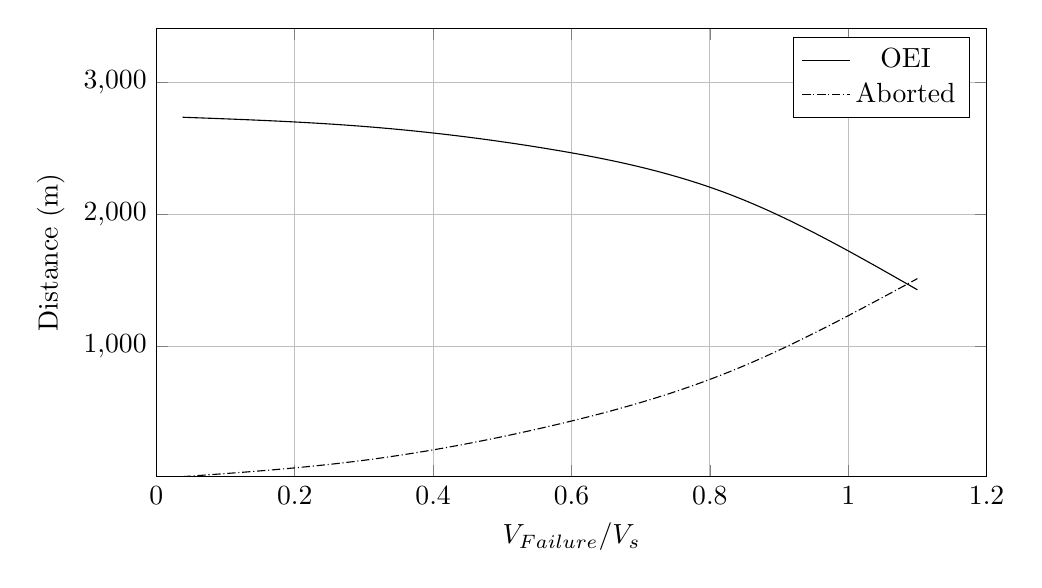
\begin{tikzpicture}

\begin{axis}[
width=\textwidth,
height=0.6\textwidth,
scaled ticks=false, tick label style={/pgf/number format/fixed},
xmin=0.0,
xmax=1.2,
xlabel={$V_{\text{Failure}}/V_s$},
xmajorgrids,
ymin=16.343983261177346,
ymax=3409.4029481001066,
ylabel={Distance (m)},
ymajorgrids,
legend entries = {OEI\\Aborted\\}
]

\addplot [
color=black,
solid
]
table[row sep=crcr]{
0.03779645082157896	2735.6611103822934\\
0.04206232852912282	2734.8398501864044\\
0.046328206236666676	2734.018095801858\\
0.050594083944210534	2733.195353039998\\
0.05485996165175439	2732.371127712165\\
0.05912583935929824	2731.5449256297034\\
0.0633917170668421	2730.716252603955\\
0.06765759477438596	2729.884614446263\\
0.07192347248192982	2729.04951696797\\
0.07618935018947369	2728.2104659804186\\
0.08045522789701755	2727.3669672949513\\
0.08472110560456142	2726.5185267229112\\
0.08898698331210528	2725.664650075641\\
0.09325286101964915	2724.8048431644834\\
0.09751873872719301	2723.9386118007806\\
0.10178461643473688	2723.0654617958758\\
0.10605049414228074	2722.1848989611117\\
0.11031637184982461	2721.296429107831\\
0.11458224955736847	2720.399558047376\\
0.11884812726491234	2719.49379159109\\
0.12311400497245621	2718.578635550315\\
0.12737988268000008	2717.6535957363944\\
0.13164576038754394	2716.718177960671\\
0.1359116380950878	2715.7718880344864\\
0.14017751580263166	2714.8142317691845\\
0.14444339351017554	2713.8447149761073\\
0.1487092712177194	2712.862843466598\\
0.15297514892526326	2711.8681230519987\\
0.15724102663280712	2710.8600595436524\\
0.161506904340351	2709.838158752902\\
0.16577278204789486	2708.8019264910904\\
0.17003865975543872	2707.7508685695598\\
0.17430453746298258	2706.684490799653\\
0.17857041517052646	2705.602298992713\\
0.18283629287807032	2704.503798960082\\
0.18710217058561418	2703.388496513103\\
0.19136804829315807	2702.255897463119\\
0.19563392600070192	2701.1055076214716\\
0.19989980370824578	2699.9368327995053\\
0.20416568141578964	2698.7493788085612\\
0.20843155912333353	2697.5426514599826\\
0.21269743683087738	2696.3161565651126\\
0.21696331453842124	2695.0693999352934\\
0.2212291922459651	2693.801887381868\\
0.225495069953509	2692.5131247161785\\
0.22976094766105284	2691.2026177495686\\
0.2340268253685967	2689.86987229338\\
0.2382927030761406	2688.5143941589563\\
0.24255858078368445	2687.1356891576393\\
0.2468244584912283	2685.7332631007725\\
0.2510903361987722	2684.3066217996984\\
0.255356213906316	2682.855271065759\\
0.2596220916138599	2681.3787167102982\\
0.2638879693214038	2679.8764645446577\\
0.2681538470289476	2678.348020380181\\
0.2724197247364915	2676.79289002821\\
0.27668560244403534	2675.210579300088\\
0.2809514801515792	2673.6005940071577\\
0.2852173578591231	2671.9624399607615\\
0.28948323556666694	2670.2956229722417\\
0.2937491132742108	2668.599648852942\\
0.2980149909817547	2666.874023414205\\
0.30228086868929854	2665.1182524673727\\
0.30654674639684243	2663.3318763287393\\
0.3108126241043863	2661.514735635469\\
0.31507850181193015	2659.6668256580265\\
0.31934437951947403	2657.7881429448366\\
0.32361025722701786	2655.878684044324\\
0.32787613493456175	2653.9384455049144\\
0.33214201264210563	2651.9674238750326\\
0.33640789034964946	2649.965615703104\\
0.34067376805719335	2647.9330175375535\\
0.34493964576473723	2645.8696259268067\\
0.34920552347228107	2643.7754374192878\\
0.35347140117982495	2641.6504485634227\\
0.35773727888736884	2639.494655907636\\
0.36200315659491267	2637.3080560003536\\
0.36626903430245655	2635.0906453899997\\
0.3705349120100004	2632.842420625\\
0.37480078971754427	2630.56337825378\\
0.37906666742508816	2628.253514824764\\
0.383332545132632	2625.9128268863774\\
0.38759842284017587	2623.5413109870456\\
0.39186430054771976	2621.1389636751933\\
0.3961301782552636	2618.705781499246\\
0.4003960559628075	2616.241761007628\\
0.40466193367035136	2613.746898748766\\
0.4089278113778952	2611.2211912710836\\
0.4131936890854391	2608.664635123007\\
0.4174595667929829	2606.077226852961\\
0.4217254445005268	2603.4589630093706\\
0.4259913222080707	2600.8098401406605\\
0.4302571999156145	2598.1298547952565\\
0.4345230776231584	2595.419003521584\\
0.4387889553307023	2592.677282868067\\
0.4430548330382461	2589.9046893831314\\
0.44732071074579	2587.1012196152024\\
0.4515865884533339	2584.2668701127045\\
0.4558524661608777	2581.4016374240637\\
0.4601183438684216	2578.505518097704\\
0.46438422157596543	2575.578508682052\\
0.4686500992835093	2572.6206057255317\\
0.4729159769910532	2569.631805776569\\
0.47718185469859703	2566.612105383588\\
0.4814477324061409	2563.561501095015\\
0.4857136101136848	2560.4799894592743\\
0.48997948782122863	2557.367567024791\\
0.4942453655287725	2554.2242303399908\\
0.4985112432363164	2551.0499759532986\\
0.5027771209438603	2547.844800413139\\
0.5070429986514041	2544.6087002679383\\
0.511308876358948	2541.3416720661203\\
0.5155747540664919	2538.043712356111\\
0.5198406317740357	2534.714817686335\\
0.5241065094815796	2531.3549846052183\\
0.5283723871891234	2527.964209661185\\
0.5326382648966673	2524.542489402661\\
0.5369041426042112	2521.089820378071\\
0.541170020311755	2517.60619913584\\
0.5454358980192989	2514.0916222243936\\
0.5497017757268428	2510.546086192157\\
0.5539676534343866	2506.9695875875545\\
0.5582335311419305	2503.3621229590117\\
0.5624994088494744	2499.723688854954\\
0.5667652865570182	2496.0542818238064\\
0.5710311642645621	2492.3538653402593\\
0.575297041972106	2488.621642183115\\
0.5795629196796498	2484.8560544352868\\
0.5838287973871937	2481.055511105952\\
0.5880946750947376	2477.2184212042907\\
0.5923605528022814	2473.3431937394807\\
0.5966264305098253	2469.4282377207005\\
0.6008923082173692	2465.471962157129\\
0.605158185924913	2461.472776057945\\
0.6094240636324568	2457.429088432327\\
0.6136899413400007	2453.339308289453\\
0.6179558190475444	2449.2018446385027\\
0.6222216967550882	2445.0151064886536\\
0.626487574462632	2440.777502849085\\
0.6307534521701758	2436.4874427289756\\
0.6350193298777196	2432.1433351375035\\
0.6392852075852634	2427.743589083848\\
0.6435510852928072	2423.286613577187\\
0.647816963000351	2418.770817626699\\
0.6520828407078948	2414.1946102415636\\
0.6563487184154386	2409.5564004309585\\
0.6606145961229823	2404.8545972040624\\
0.6648804738305262	2400.0876095700546\\
0.66914635153807	2395.253846538113\\
0.6734122292456138	2390.3517171174162\\
0.6776781069531576	2385.3796303171434\\
0.6819439846607014	2380.3359951464727\\
0.6862098623682452	2375.2192206145833\\
0.6904757400757889	2370.0277157306527\\
0.6947416177833328	2364.759889503861\\
0.6990074954908766	2359.4141509433853\\
0.7032733731984204	2353.988909058405\\
0.7075392509059641	2348.482572858099\\
0.711805128613508	2342.893551351646\\
0.7160710063210518	2337.2202535482234\\
0.7203368840285955	2331.4610884570106\\
0.7246027617361394	2325.614465087186\\
0.7288686394436832	2319.678792447929\\
0.733134517151227	2313.6524795484174\\
0.7374003948587707	2307.5339353978297\\
0.7416662725663146	2301.3215690053453\\
0.7459321502738584	2295.013789380142\\
0.7501980279814021	2288.609005531399\\
0.754463905688946	2282.1056264682943\\
0.7587297833964898	2275.502061200007\\
0.7629956611040336	2268.796718735716\\
0.7672615388115773	2261.9880080845987\\
0.7715274165191212	2255.0743382558353\\
0.775793294226665	2248.054118258603\\
0.7800591719342087	2240.9257571020817\\
0.7843250496417525	2233.6876637954488\\
0.7885909273492964	2226.338247347883\\
0.7928568050568402	2218.8759167685644\\
0.7971226827643839	2211.29908106667\\
0.8013885604719277	2203.606149251379\\
0.8056544381794716	2195.7955303318704\\
0.8099203158870153	2187.865633317322\\
0.8141861935945591	2179.8148672169127\\
0.818452071302103	2171.6416410398215\\
0.8227179490096468	2163.344363795227\\
0.8269838267171905	2154.921444492307\\
0.8312497044247343	2146.3712921402407\\
0.8355155821322782	2137.6923253305554\\
0.8397814598398219	2128.8841221189628\\
0.8440473375473657	2119.9485124131033\\
0.8483132152549095	2110.8875848440307\\
0.8525790929624534	2101.7034280427984\\
0.8568449706699971	2092.39813064046\\
0.8611108483775409	2082.9737812680683\\
0.8653767260850848	2073.432468556678\\
0.8696426037926285	2063.7762811373423\\
0.8739084815001723	2054.007307641115\\
0.8781743592077161	2044.1276366990487\\
0.88244023691526	2034.1393569421975\\
0.8867061146228037	2024.0445570016154\\
0.8909719923303475	2013.8453255083555\\
0.8952378700378913	2003.5437510934712\\
0.8995037477454351	1993.1419223880164\\
0.9037696254529789	1982.6419280230446\\
0.9080355031605227	1972.0458566296093\\
0.9123013808680666	1961.355796838764\\
0.9165672585756103	1950.5738372815622\\
0.9208331362831541	1939.7020665890575\\
0.9250990139906979	1928.7425733923037\\
0.9293648916982417	1917.6974463223542\\
0.9336307694057855	1906.5687740102621\\
0.9378966471133293	1895.3586450870819\\
0.942162524820873	1884.0691481838662\\
0.9464284025284169	1872.7023719316692\\
0.9506942802359607	1861.2604049615443\\
0.9549601579435045	1849.7453359045448\\
0.9592260356510482	1838.1592533917244\\
0.9634919133585921	1826.504246054137\\
0.9677577910661359	1814.7824025228356\\
0.9720236687736796	1802.995811428874\\
0.9762895464812235	1791.146561403306\\
0.9805554241887673	1779.2367410771844\\
0.9848213018963111	1767.2684390815637\\
0.9890871796038548	1755.2437440474969\\
0.9933530573113987	1743.1647446060379\\
0.9976189350189425	1731.0335293882397\\
1.0018848127264863	1718.8521870251561\\
1.00615069043403	1706.622806147841\\
1.0104165681415738	1694.3474753873477\\
1.0146824458491177	1682.0282833747297\\
1.0189483235566614	1669.6673187410406\\
1.0232142012642054	1657.266670117334\\
1.027480078971749	1644.8284261346635\\
1.0317459566792928	1632.3546754240822\\
1.0360118343868367	1619.8475066166443\\
1.0402777120943805	1607.309008343403\\
1.0445435898019242	1594.741269235412\\
1.0488094675094681	1582.146377923725\\
1.0530753452170118	1569.526423039395\\
1.0573412229245556	1556.883493213476\\
1.0616071006320995	1544.2196770770215\\
1.0658729783396432	1531.5370632610848\\
1.070138856047187	1518.8377403967197\\
1.074404733754731	1506.1237971149799\\
1.0786706114622746	1493.3973220469188\\
1.0829364891698186	1480.6604038235898\\
1.0872023668773623	1467.9151310760467\\
1.091468244584906	1455.1635924353427\\
1.09573412229245	1442.4078765325316\\
1.0999999999999999	1429.6500719986484\\
};

\addplot [
color=black,
densely dashdotted
]
table[row sep=crcr]{
0.03779645082157896	15.554718447147376\\
0.04206232852912282	17.137506450324782\\
0.046328206236666676	18.720981278264468\\
0.050594083944210534	20.30582975572871\\
0.05485996165175439	21.892738707479786\\
0.05912583935929824	23.482394958279976\\
0.0633917170668421	25.07548533289156\\
0.06765759477438596	26.672696656076816\\
0.07192347248192982	28.27471575259802\\
0.07618935018947369	29.882229447217455\\
0.08045522789701755	31.495924564697397\\
0.08472110560456142	33.116487929800115\\
0.08898698331210528	34.74460636728791\\
0.09325286101964915	36.38096670192304\\
0.09751873872719301	38.02625575846779\\
0.10178461643473688	39.68116036168444\\
0.10605049414228074	41.34636733633526\\
0.11031637184982461	43.022563507182554\\
0.11458224955736847	44.71043569898856\\
0.11884812726491234	46.41067073651559\\
0.12311400497245621	48.12395544452592\\
0.12737988268000008	49.850976647781806\\
0.13164576038754394	51.592421171045544\\
0.1359116380950878	53.3489758390794\\
0.14017751580263166	55.121327476645675\\
0.14444339351017554	56.91016290850662\\
0.1487092712177194	58.716168959424536\\
0.15297514892526326	60.54003245416169\\
0.15724102663280712	62.382440217480365\\
0.161506904340351	64.24407907414285\\
0.16577278204789486	66.12563584891139\\
0.17003865975543872	68.02779736654828\\
0.17430453746298258	69.95125045181582\\
0.17857041517052646	71.89668192947627\\
0.18283629287807032	73.8647786242919\\
0.18710217058561418	75.856227361025\\
0.19136804829315807	77.87171496443786\\
0.19563392600070192	79.91192825929274\\
0.19989980370824578	81.97755407035191\\
0.20416568141578964	84.06927922237767\\
0.20843155912333353	86.1877905401323\\
0.21269743683087738	88.33377484837806\\
0.21696331453842124	90.50791897187723\\
0.2212291922459651	92.71090973539211\\
0.225495069953509	94.94343396368495\\
0.22976094766105284	97.20617848151805\\
0.2340268253685967	99.49983011365369\\
0.2382927030761406	101.82507568485413\\
0.24255858078368445	104.18260201988166\\
0.2468244584912283	106.57309594349856\\
0.2510903361987722	108.9972442804671\\
0.255356213906316	111.45573385554957\\
0.2596220916138599	113.94925149350824\\
0.2638879693214038	116.47848401910538\\
0.2681538470289476	119.04411825710332\\
0.2724197247364915	121.64684103226425\\
0.27668560244403534	124.2873391693505\\
0.2809514801515792	126.96629949312437\\
0.2852173578591231	129.6844088283481\\
0.28948323556666694	132.442353999784\\
0.2937491132742108	135.2408218321943\\
0.2980149909817547	138.08049915034132\\
0.30228086868929854	140.96207277898733\\
0.30654674639684243	143.88616732465027\\
0.3108126241043863	146.85286586468416\\
0.31507850181193015	149.86197264653316\\
0.31934437951947403	152.91328961326204\\
0.32361025722701786	156.0066187079355\\
0.32787613493456175	159.1417618736183\\
0.33214201264210563	162.31852105337515\\
0.33640789034964946	165.5366981902708\\
0.34067376805719335	168.79609522737002\\
0.34493964576473723	172.0965141077375\\
0.34920552347228107	175.437756774438\\
0.35347140117982495	178.81962517053623\\
0.35773727888736884	182.24192123909697\\
0.36200315659491267	185.70444692318492\\
0.36626903430245655	189.20700416586482\\
0.3705349120100004	192.74939491020143\\
0.37480078971754427	196.33142109925944\\
0.37906666742508816	199.95288467610362\\
0.383332545132632	203.61358758379873\\
0.38759842284017587	207.31333176540946\\
0.39186430054771976	211.05191916400054\\
0.3961301782552636	214.82915172263677\\
0.4003960559628075	218.64483138438283\\
0.40466193367035136	222.49876009230348\\
0.4089278113778952	226.39073978946342\\
0.4131936890854391	230.32057241892744\\
0.4174595667929829	234.28805992376024\\
0.4217254445005268	238.29300424702657\\
0.4259913222080707	242.33520733179117\\
0.4302571999156145	246.41447112111877\\
0.4345230776231584	250.53059755807408\\
0.4387889553307023	254.68338858572187\\
0.4430548330382461	258.8726461471269\\
0.44732071074579	263.0981721853538\\
0.4515865884533339	267.3597686434674\\
0.4558524661608777	271.6572374645325\\
0.4601183438684216	275.99038059161364\\
0.46438422157596543	280.35899996777573\\
0.4686500992835093	284.7628975360834\\
0.4729159769910532	289.20187523960146\\
0.47718185469859703	293.67573502139464\\
0.4814477324061409	298.1842788245276\\
0.4857136101136848	302.72730859206524\\
0.48997948782122863	307.3046262670721\\
0.4942453655287725	311.916033792613\\
0.4985112432363164	316.5613331117527\\
0.5027771209438603	321.24032616755585\\
0.5070429986514041	325.9528149030873\\
0.511308876358948	330.6986012614117\\
0.5155747540664919	335.4774871855939\\
0.5198406317740357	340.2892746186984\\
0.5241065094815796	345.13376550379024\\
0.5283723871891234	350.01076178393396\\
0.5326382648966673	354.9200654021944\\
0.5369041426042112	359.8614783016361\\
0.541170020311755	364.834802425324\\
0.5454358980192989	369.8398397163229\\
0.5497017757268428	374.87639211769726\\
0.5539676534343866	379.944261572512\\
0.5582335311419305	385.0432500238319\\
0.5624994088494744	390.17315941472157\\
0.5667652865570182	395.3337916882457\\
0.5710311642645621	400.5249748602293\\
0.575297041972106	405.7471366199788\\
0.5795629196796498	411.0013043302824\\
0.5838287973871937	416.28853142668856\\
0.5880946750947376	421.6098713447455\\
0.5923605528022814	426.96637752000163\\
0.5966264305098253	432.3591033880053\\
0.6008923082173692	437.7891023843048\\
0.605158185924913	443.25742794444847\\
0.6094240636324568	448.76513350398454\\
0.6136899413400007	454.3132724984615\\
0.6179558190475444	459.90289836342765\\
0.6222216967550882	465.5350645344313\\
0.626487574462632	471.2108244470208\\
0.6307534521701758	476.9312315367445\\
0.6350193298777196	482.6973392391507\\
0.6392852075852634	488.5102009897878\\
0.6435510852928072	494.3708702242041\\
0.647816963000351	500.28040037794796\\
0.6520828407078948	506.23984488656765\\
0.6563487184154386	512.2502571856115\\
0.6606145961229823	518.312690710628\\
0.6648804738305262	524.4281988971653\\
0.66914635153807	530.5978351807719\\
0.6734122292456138	536.822652996996\\
0.6776781069531576	543.103705781386\\
0.6819439846607014	549.4420469694902\\
0.6862098623682452	555.838729996857\\
0.6904757400757889	562.2948082990346\\
0.6947416177833328	568.8113353115715\\
0.6990074954908766	575.389364470016\\
0.7032733731984204	582.0299492099164\\
0.7075392509059641	588.734142966821\\
0.711805128613508	595.5029991762781\\
0.7160710063210518	602.3375712738361\\
0.7203368840285955	609.2389126950435\\
0.7246027617361394	616.2080768754485\\
0.7288686394436832	623.2461172505994\\
0.733134517151227	630.3540872560443\\
0.7374003948587707	637.5330403273321\\
0.7416662725663146	644.7840299000106\\
0.7459321502738584	652.1081094096286\\
0.7501980279814021	659.506332291734\\
0.754463905688946	666.9797519818753\\
0.7587297833964898	674.529421915601\\
0.7629956611040336	682.1563955284594\\
0.7672615388115773	689.8617262559985\\
0.7715274165191212	697.646467533767\\
0.775793294226665	705.5116727973132\\
0.7800591719342087	713.4583954821852\\
0.7843250496417525	721.4876890239316\\
0.7885909273492964	729.6006068581005\\
0.7928568050568402	737.7982024202404\\
0.7971226827643839	746.0815291458996\\
0.8013885604719277	754.4516404706264\\
0.8056544381794716	762.9095898299693\\
0.8099203158870153	771.4564306594764\\
0.8141861935945591	780.0932163946961\\
0.818452071302103	788.8210004711768\\
0.8227179490096468	797.6408363244668\\
0.8269838267171905	806.5537773901145\\
0.8312497044247343	815.5608771036682\\
0.8355155821322782	824.6631821411997\\
0.8397814598398219	833.8609212821412\\
0.8440473375473657	843.1527348289792\\
0.8483132152549095	852.5370805783381\\
0.8525790929624534	862.0124163268426\\
0.8568449706699971	871.5771998711176\\
0.8611108483775409	881.2298890077875\\
0.8653767260850848	890.968941533477\\
0.8696426037926285	900.7928152448109\\
0.8739084815001723	910.6999679384136\\
0.8781743592077161	920.6888574109099\\
0.88244023691526	930.7579414589245\\
0.8867061146228037	940.9056778790818\\
0.8909719923303475	951.1305244680068\\
0.8952378700378913	961.430939022324\\
0.8995037477454351	971.8053793386579\\
0.9037696254529789	982.2523032136334\\
0.9080355031605227	992.7701684438749\\
0.9123013808680666	1003.3574328260072\\
0.9165672585756103	1014.0125541566549\\
0.9208331362831541	1024.7339902324427\\
0.9250990139906979	1035.5201988499953\\
0.9293648916982417	1046.3696378059371\\
0.9336307694057855	1057.280764896893\\
0.9378966471133293	1068.2520379194877\\
0.942162524820873	1079.2819146703457\\
0.9464284025284169	1090.3688529460915\\
0.9506942802359607	1101.5113105433502\\
0.9549601579435045	1112.707745258746\\
0.9592260356510482	1123.9566148889035\\
0.9634919133585921	1135.256377230448\\
0.9677577910661359	1146.6054900800034\\
0.9720236687736796	1158.0024112341946\\
0.9762895464812235	1169.4455984896465\\
0.9805554241887673	1180.9335096429836\\
0.9848213018963111	1192.4646024908304\\
0.9890871796038548	1204.0373348298117\\
0.9933530573113987	1215.6501644565521\\
0.9976189350189425	1227.3015491676763\\
1.0018848127264863	1238.9899467598088\\
1.00615069043403	1250.7138150295746\\
1.0104165681415738	1262.471611773598\\
1.0146824458491177	1274.2617947885037\\
1.0189483235566614	1286.0828218709164\\
1.0232142012642054	1297.933150817461\\
1.027480078971749	1309.8112394247617\\
1.0317459566792928	1321.7155454894432\\
1.0360118343868367	1333.6445268081306\\
1.0402777120943805	1345.5966411774482\\
1.0445435898019242	1357.5703463940206\\
1.0488094675094681	1369.5641002544726\\
1.0530753452170118	1381.576360555429\\
1.0573412229245556	1393.605585093514\\
1.0616071006320995	1405.6502316653527\\
1.0658729783396432	1417.7087580675693\\
1.070138856047187	1429.779622096789\\
1.074404733754731	1441.8612815496358\\
1.0786706114622746	1453.9521942227352\\
1.0829364891698186	1466.050817912711\\
1.0872023668773623	1478.1556104161882\\
1.091468244584906	1490.2650295297915\\
1.09573412229245	1502.3775330501455\\
1.0999999999999999	1514.4915787738928\\
};
\end{axis}
\end{tikzpicture}%

\caption{Balanced take-off length chart - ATR-72}
\end{figure}
%
\noindent
In conclusion of the take-off analysis, it's useful to highlight the effects that $k_{\alpha}$ and $\alpha_{\text{red}}$ have on the take-off run. The first one influences the rotation phase making the pilot's maneuver faster as it grows; in particular, from figure \ref{fig:kAlphaEffects}, a faster rotation maneuver makes $\alpha$ to rise faster reaching the limit angle (related to the $C_L$ limitation imposed) before with the effect of having a high drag for more time so that the take-off run is longer. The second parameter influences the airborne phase making the reduction in angle of attack faster as it grows; the result is that the load factor reaches the value of 1 later (eventually never) and so the rate of climb is higher making the airborne phase to be shorter with a lower value of the take-off run (see figures \ref{fig:CLAlphaRED}, \ref{fig:LoadFactorAlphaRED} and \ref{fig:RateOfClimbAlphaRED}).
%
\begin{figure}[!b]
\centering
\includegraphics[keepaspectratio, width=1.07\textwidth]{Angles_vs_GroundDistance_KAlpha}
\caption{Effect of $\alpha_{\text{red}}$ on the $C_L$ during the airborne phase - ATR-72}
\label{fig:kAlphaEffects}
\end{figure}
%
\begin{figure}[H]
\centering
\includegraphics[keepaspectratio, width=1.05\textwidth]{CL_vs_GroundDistance_AlphaRED}
\caption{Effect of $\alpha_{\text{red}}$ on the load factor during the airborne phase - ATR-72}
\label{fig:CLAlphaRED}
\end{figure}
%
\begin{figure}[H]
\centering
\includegraphics[keepaspectratio, width=1.05\textwidth]{LoadFactor_vs_GroundDistance_AlphaRED}
\caption{Effect of $\alpha_{\text{red}}$ on the rate of climb during the airborne phase - ATR-72}
\label{fig:LoadFactorAlphaRED}
\end{figure}
%
\begin{figure}[H]
\centering
\includegraphics[keepaspectratio, width=1.05\textwidth]{RateOfClimb_vs_GroundDistance_AlphaRED}
\caption{Effect of $k_{\alpha}$ on the rotation phase - ATR-72}
\label{fig:RateOfClimbAlphaRED}
\end{figure}
%
%--------------------------------Landing Charts------------------------------------------
%
\begin{figure}[!t]
\centering
\includegraphics[keepaspectratio, width=1.05\textwidth]{TrajectoryAndSpeed_vs_GroundDistance_LANDING}
\caption{Landing trajectory and speed evolution with \lstinline[language=Java]!phiRev!=0.0 - ATR-72}
\label{fig:Landing1}
\end{figure}
%
\begin{figure}[!b]
\centering
\includegraphics[keepaspectratio, width=1.05\textwidth]{TrajectoryAndSpeed_vs_GroundDistance_LANDING_REV}
\caption{Landing trajectory and speed evolution with \lstinline[language=Java]!phiRev!=0.25 - ATR-72}
\end{figure}
%
\begin{figure}[!t]
\centering
\includegraphics[keepaspectratio, width=1.1\textwidth]{HorizontalForces_vs_GroundDistance_LANDING}
\caption{Forces evolution in landing, during the ground run, with \lstinline[language=Java]!phiRev!=0.0 - ATR-72}
\end{figure}
%
\begin{figure}[!b]
\centering
\includegraphics[keepaspectratio, width=1.1\textwidth]{HorizontalForces_vs_GroundDistance_LANDING_REV}
\caption{Forces evolution in landing, during the ground run, with \lstinline[language=Java]!phiRev!=0.25 - ATR-72}
\end{figure}
%
\begin{figure}[!t]
\centering
%Acceleration_vs_GroundDistance
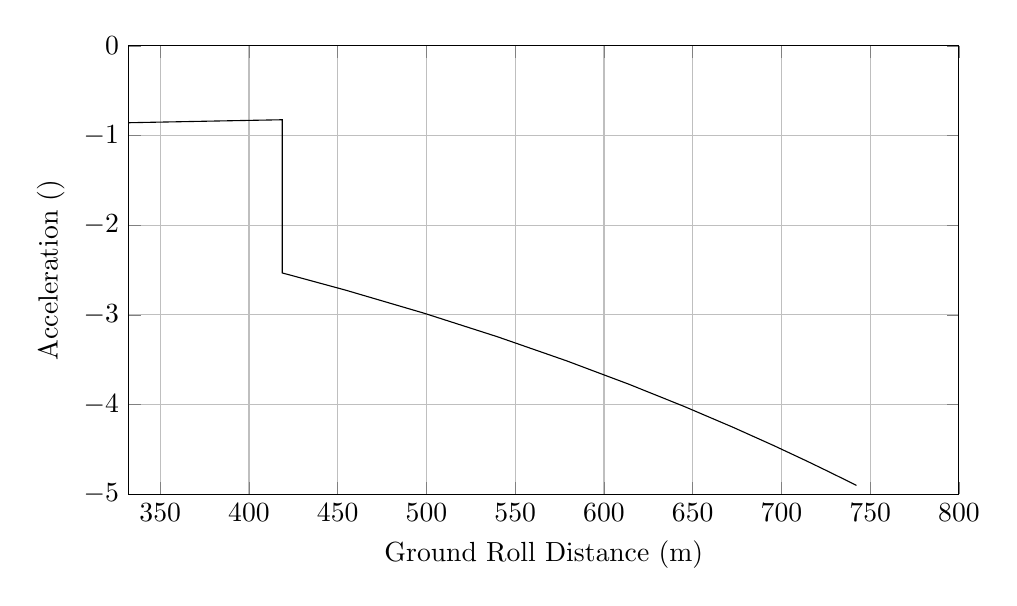
\begin{tikzpicture}

\begin{axis}[
width=\textwidth,
height=0.6\textwidth,
scaled ticks=false, tick label style={/pgf/number format/fixed},
xmin=332.24668448543065,
xmax=800,
xlabel={Ground Roll Distance (m)},
xmajorgrids,
ymin=-5,
ymax=0,
ylabel={Acceleration ($\si{\meter\per\square\second}$)},
ymajorgrids,
legend style={at={(1.03,0.5)},anchor=west,draw=black,fill=white,legend cell align=left}
]

\addplot [
color=black,
solid
]
table[row sep=crcr]{
271.1027384946931	-0.8821769415091307\\
278.1830410948079	-0.8793279191382144\\
328.35777746809856	-0.8594001664513955\\
377.6730485624604	-0.8402538971220281\\
387.43466541350995	-0.8365149028917145\\
397.16282157054764	-0.8328052776744466\\
406.85766541958094	-0.8291247218528386\\
416.5193441838287	-0.8254729396486338\\
418.44771300098773	-0.8247460102801847\\
418.6019254845137	-0.8246879050769627\\
418.6636081133455	-0.8246646650327947\\
418.70180389309803	-0.8246502744114361\\
418.71916593278456	-0.8246437331817544\\
418.73613530509124	-0.8246373399414841\\
418.74628077897705	-0.824633517640383\\
418.7496319594153	-0.8246322550890883\\
418.75066763163716	-0.8246318649018045\\
418.7512660131255	-0.8246316394629487\\
418.7516244078647	-2.533551162490217\\
418.75195284655274	-2.533552860937582\\
418.7552372269603	-2.533569845440372\\
418.7880803836774	-2.533739693382852\\
419.116447199047	-2.535438464088604\\
422.3936241004501	-2.5524551212363846\\
454.5000625074308	-2.7253277463276477\\
498.52736946937296	-2.981580685716774\\
540.1148050616696	-3.2457239568092815\\
578.7489528684882	-3.512033628201375\\
613.8715048262088	-3.7730530397821394\\
645.2219757903133	-4.022382893599108\\
672.5516108973475	-4.253139759454994\\
695.630241697474	-4.45828279902468\\
714.2532936419457	-4.631012387338757\\
726.7418879467689	-4.75057749229979\\
735.6228963049912	-4.83747730837846\\
740.4862872809363	-4.885736876779081\\
742.139843659711	-4.902254598301262\\
742.2468071484855	-4.903324999999999\\
};
\end{axis}
\end{tikzpicture}%

\caption{Acceleration evolution in landing, during the ground run, with \lstinline[language=Java]!phiRev!=0.0 - ATR-72}
\end{figure}
%
\begin{figure}[!b]
\centering
%Acceleration_vs_GroundDistance
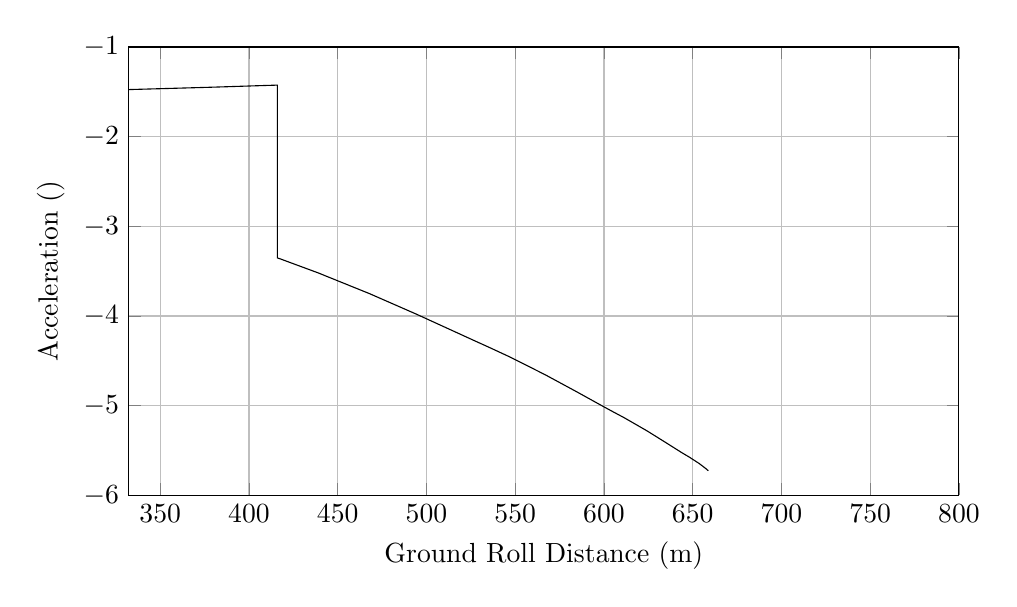
\begin{tikzpicture}

\begin{axis}[
width=\textwidth,
height=0.6\textwidth,
scaled ticks=false, tick label style={/pgf/number format/fixed},
xmin=332.24668448543065,
xmax=800,
xlabel={Ground Roll Distance (m)},
xmajorgrids,
ymin=-6,
ymax=-1,
ylabel={Acceleration ($\si{\meter\per\square\second}$)},
ymajorgrids,
legend style={at={(1.03,0.5)},anchor=west,draw=black,fill=white,legend cell align=left}
]

\addplot [
color=black,
solid
]
table[row sep=crcr]{
271.1015686690888	-1.505826897495529\\
278.16352829882203	-1.5025108868832273\\
327.93189208610966	-1.4778393344070122\\
376.22263522333753	-1.4505541052577144\\
385.70581903369396	-1.4446671973420635\\
395.1312167074841	-1.4386149116315758\\
404.499069977291	-1.4325561663276631\\
407.22317284616634	-1.43084049506436\\
412.6567497046	-1.4274810867756185\\
414.51342082390977	-1.4263520108357945\\
415.25545016494675	-1.4259034186858242\\
415.552159686178	-1.4257244650830199\\
415.67789440634897	-1.425648703539932\\
415.92933237969885	-1.4254973287057138\\
415.9501295181409	-1.4254848157831894\\
415.9608938122816	-1.4254783397404758\\
415.9660652984825	-1.425475228569681\\
415.9671664536253	-1.4254745661231518\\
415.96791210385766	-1.4254741175475392\\
415.9681120960404	-3.352112548149041\\
415.9683218158177	-3.352114007557268\\
415.9704190098155	-3.352128601681235\\
415.99139057223	-3.3522745470911888\\
416.2010684339259	-3.3537344179713795\\
418.29406471436175	-3.3683745547749213\\
438.8396181683647	-3.518639986870509\\
467.96299828918427	-3.7515874001739924\\
494.1517076274454	-3.978585253794746\\
517.7426126590012	-4.191833093854532\\
527.4373605384853	-4.279673880147625\\
534.9959724450205	-4.347272526781998\\
546.8225215414291	-4.455889484041267\\
566.9088739987865	-4.65593143445369\\
584.6364791819944	-4.845702183928733\\
600.2447078462001	-5.016595748749857\\
605.2885947877262	-5.070669030714422\\
608.5760104703779	-5.105136897046094\\
611.5622302447002	-5.136885530165669\\
624.2835724517483	-5.281869470965937\\
634.9837906896055	-5.414002587643369\\
643.753118395183	-5.52353592191726\\
645.9782216377341	-5.549886519159289\\
646.9408184990989	-5.56088972518285\\
647.8610688046081	-5.571558900816601\\
653.6946345451113	-5.646374636757027\\
657.4138215620001	-5.702667310069476\\
658.4847028046415	-5.720928726189506\\
658.710097175273	-5.72499331736185\\
658.8167646729503	-5.726970049979389\\
658.8273823577272	-5.72717080913929\\
};
\end{axis}
\end{tikzpicture}%

\caption{Acceleration evolution in landing, during the ground run, with \lstinline[language=Java]!phiRev!=0.25 - ATR-72}
\end{figure}
%
\begin{figure}[!b]
\centering
\includegraphics[keepaspectratio, width=1.03\textwidth]{LoadFactor_vs_GroundDistance_LANDING}
\caption{Load factor evolution in landing, during the ground run, with \lstinline[language=Java]!phiRev!=0.0 - ATR-72}
\end{figure}
%
\begin{figure}[!b]
\centering
\includegraphics[keepaspectratio, width=1.03\textwidth]{LoadFactor_vs_GroundDistance_LANDING_REV}
\caption{Load factor evolution in landing, during the ground run, with \lstinline[language=Java]!phiRev!=0.25 - ATR-72}
\label{fig:LandingEnd}
\end{figure}
%
%----------------------- CASE STUDY : B747-100B SENSIBILITY ANALYSIS -------------------------
%
\clearpage
%
\section{Case study: B747-100B}
%
In conclusion, after having shown that the classes \lstinline[language=Java]!CalcTakeOff! and \lstinline[language=Java]!CalcLanding! work correctly, it's interesting to examine how these classes behaves when analyzing a transport jet such as the B747-100B. In particular, the analysis that will be shown and commented will regard a sensibility analysis of the \gls{FAR}-25 take-off and field length with respect to two main design parameters like the wing loading $\frac{W}{S}$, for both take-off and landing, and the thrust ratio $\frac{T}{W}$, for the take-off only.

\bigskip
\noindent
Starting from the flight manual data regarding the maximum take-off and landing weight, and knowing the wing geometry, the two wing loadings, in both take-off and landing conditions, has been derived. From these values a variation of these latter from a -10\% to a +20\% has been assigned obtaining the following results.  
%


